%=============================================================%
\author{Matteo Dall'Amico}
%=============================================================%
%*******************Dichiarazione della classe di documento e pacchetti usati***********
\documentclass[11pt,a4paper,english]{book}  %uso carta a4 e dimnesione font: 11 punti, tipo di documento
\usepackage[latin1]{inputenc}
%\usepackage[T1]{fontenc}
\usepackage[english]{babel}
\usepackage{fancyhdr}

%\usepackage{sfchap}
%\usepackage{graphicx}
\usepackage{longtable,lscape}
\usepackage{caption}

\usepackage[usenames]{color}
\usepackage{times}

\usepackage{setspace}
\usepackage{makeidx}


\usepackage{hyperref}
\hypersetup{ %hyperref setup
    bookmarks=true,         % show bookmarks bar?
    unicode=false,          % non-Latin characters in Acrobat�s bookmarks
    pdftoolbar=true,        % show Acrobat�s toolbar?
    pdfmenubar=true,        % show Acrobat�s menu?
    pdffitwindow=false,     % window fit to page when opened
    pdfstartview={FitH},    % fits the width of the page to the window
    pdftitle={},    % title
    pdfauthor={},     % author
    pdfsubject={},   % subject of the document
    pdfcreator={-},   % creator of the document
    pdfproducer={-}, % producer of the document
    pdfkeywords={-}, % list of keywords
    pdfnewwindow=true,      % links in new window
    colorlinks=true,       % false: boxed links; true: colored links
    linkcolor=blue,          % color of internal links
    citecolor=blue,        % color of links to bibliography
    filecolor=blue,      % color of file links
    urlcolor=blue           % color of external links
}

%%%%%%%%%%%%%%%%%%%%%%%%%%%%%%%%%% userpakage ex Fraccarollo %%%%%%%%%%%%%%%%%%%%
%\usepackage{wsuipa}
\usepackage{amsmath}
\usepackage{textcomp}
%\usepackage[T1]{fontenc}
\usepackage{float}
%\usepackage{colortbl}
\usepackage{fancyhdr}
%\usepackage{longtable}
%\usepackage[tcidvi]{graphicx}
\usepackage{amsfonts}
\usepackage{amssymb}
%\usepackage{setspace}
%\usepackage{caption}
\usepackage{float}
\usepackage{subfig}
\usepackage{lastpage}
\usepackage{natbib} % per mettere year, title or whatever you want for the bibliograpy

%\usepackage{chicago}%
%\usepackage{graphicx}
%%%%%%%%%%%%%%%%%%%%%%%%%%%%%%%%%%%%%%%%%%%%%%%%%%%
\newif\ifpdf
\ifx\pdfoutput\undefined
\pdffalse % we are not running PDFLaTeX
\else
\pdfoutput=1 % we are running PDFLaTeX
\pdftrue
\fi

\ifpdf
\usepackage[pdftex]{graphicx}
\else
\usepackage{graphicx}
%\usepackage{graphicx}
\fi

%*****************Tutta una serie di comandi di formattazione**************************
\textwidth=16.5cm %larghezza corpo testo (l'intero paragrafo, non le parole singole)
\textheight=23cm %altezza del corpo del testo (spazio occupato)
\headsep=1cm %distanza del testo dall'intestazione in alto
\topmargin=1.5cm %distanza dell'intestazione dal limite superiore (che non � il margine)*
\footskip=1cm %distanza tra il testo e il piede di pagina inferiore
\voffset=-2cm %zona tra il limite superiore e il margine del foglio (vedi manuale)
\evensidemargin=-0.50cm
\oddsidemargin=0cm


%\providecommand{\geotop}{\lower-.25em\hbox{G}E\lower.25em\hbox{O}\lower-.25em\hbox{T}O\lower-.25em\hbox{P}\@}

\makeindex  %per fare l'indice analitico

%*****************Inizio descrizione del testo: indice, capitoli, elenchi**************

\begin{document}


%%% TITOLO%%%%%%%%%%%%%%%%%%%%%%%%%%%%%%%

\begin{titlepage}
\thispagestyle{empty}
\topmargin=0cm


\vspace{1cm}
\begin{center}
{\Huge GEOtop Users Manual \\}
%\vspace{0.2cm}
%{\huge a protezione del traffico autostradale da colate di detriti\\}
%\vspace{0.2cm}
%{\huge km 31+600 - 34+400\\}

%\vspace{2cm}
%{\huge Progetto di Dettaglio}
%\vspace{2.5cm}

\begin{figure}[htbp]
\begin{center}

\includegraphics[width=8.cm]{./images/titlepage/GEOtop_R.pdf}\\
\vspace{0.5cm}
\end{center}
\end{figure}



%{\large{\bf Mountain-eering S.r.l.}}\\ \vspace{0.2cm} 
%{ Societ\`a di Ingegneria}\\ 
%{ Via Siemens 19 - 39100 Bolzano}
\end{center}

%\vspace{0.5cm}


\begin{table}[h!]
\centering
\begin{tabular}{lp{3cm}l}
 \scshape{} 	& & \scshape{Edition by:} \\ \\
 \textsl{}	& & \textsl{Dr Stefano Endrizzi$^1$} \\
 						& & \textsl{Dr Matteo Dall'Amico$^2$} \\
 						& & \textsl{Dr Stefano Cozzini$^3$} \\
 						& & \textsl{Dr Emanuele Cordano$^4$} \\
 						& & \textsl{Dr Stephan Gruber$^1$} \\
						& & \textsl{Prof Riccardo Rigon$^5$} \\
\end{tabular}
\end{table}

\vspace{2.0cm}
\noindent $^1$: {\footnotesize Department of Physical Geography, University of Zurich (Switzerland)}\\
\noindent $^2$: {\footnotesize Mountain-eering S.r.l., Via Siemens 19 Bolzano (Italy)}\\
\noindent $^3$: {\footnotesize eXact-lab S.r.l., Via Beirut 2/4 Trieste (Italy)}\\
\noindent $^4$: {\footnotesize Rendena100 di Cordano Emanuele, Via Durone 3 Tione di Trento (Italy)}\\
\noindent $^5$: {\footnotesize Department of Civil and Environmental Engineering, University of Trento (Italy)}
%=========
\begin{center}
\vspace{3.0cm}
{\large User Manual for GEOtop 2.1 }

\vspace{1cm}

{\large Last revision: April 2017}
\end{center}

\clearpage

\thispagestyle{empty}

\vspace{1cm}

\mbox{ } \thispagestyle{empty}

\end{titlepage}


%*********************Fine modifica titolo******************************************

\baselineskip=6mm %formattazione distanza tra le linee del testo

\pagenumbering{roman} \setcounter{page}{1}
\tableofcontents %questo genera l'indice

%\clearpage

%**************************NUOVA FORMATTAZIONE TITOLI E PARAGRAFI E SPAZIATURA TRA PARAGRAFI*****
%\makeatletter %setto la @ come font comando

%\renewcommand{\chapter}{\@startsection  %formattazione titolo capitolo
 %      {chapter}                            %nome
%       {0}                                  %livello
%       {0mm}                                %rientro
%       {10cm}                               %spazio prima
%       {1cm}                              %spazio dopo
%       {\normalfont\huge\bfseries\upshape}} %formattazione carattere

%\renewcommand{\section}{\@startsection  %formattazione titolo sezione
%       {section}                            %nome
%       {1}                                  %livello
%       {0mm}                                %rientro
%       {2cm}                                %spazio prima
%       {1cm}                                %spazio dopo
%       {\normalfont\LARGE\bfseries\upshape}}%formattazione carattere

%\renewcommand{\subsection}{\@startsection  %formattazione titolo subsezione
%       {subsection}                           %nome
%       {2}                                         %livello
%       {0mm}                                  %rientro
%      {1.5cm}                                %spazio prima
%       {0.5cm}                                %spazio dopo
 %      {\normalfont\Large\bfseries\upshape}}  %formattazione carattere

%\renewcommand{\subsubsection}{\@startsection  %formattazione titolo subsubsezione
%       {subsubsection}                        %nome
%       {3}                                    %livello
%       {0mm}                                  %rientro
%       {1.5cm}                                %spazio prima
%       {0.5cm}                                %spazio dopo
%       {\normalfont\large\bfseries\upshape}}  %formattazione carattere

%\renewcommand{\paragraph}{\@startsection      %formattazione titolo paragraph
%       {paragraph}                            %nome
%       {4}                                    %livello
%       {0mm}                                  %rientro
%       {1cm}                                  %spazio prima
%       {0.7cm}                                %spazio dopo
%       {\normalfont\normalsize\itshape}}      %formattazione carattere

%\makeatother %riporto la @ a font normale
%**************************FINE FORMATTAZIONE TITOLI E PARAGRAFI E SPAZIATURA TRA PARAGRAFI*****

\parindent=0.5cm %formattaz. rientro dell'inizio paragrafo
%\newpage
%\clearpage
\mbox{ }  \thispagestyle{empty}
\pagenumbering{arabic} \setcounter{page}{1} %numerazioni pagine (testo)

%\clearpage
%\newpage
\pagestyle{fancy} %stile di formattazione di pagina (per l'intestazione eil pi� del documento)
\fancyhead[LE,RO]{\footnotesize \slshape {\leftmark}} %formattazione intestazione (vedi man.)
\fancyhead[LO,RE]{\footnotesize \slshape \rightmark } %come sopra (vedi manuale)
%\fancyfoot[LE,RO]{\footnotesize \slshape {Mountain-eering S.r.l. \\ Societ\`a di Ingegneria}} 
%\fancyfoot[RE,LO]{\footnotesize \slshape {www.mountain-eering.com \\ info@mountain-eering.com}} 
\fancyfoot[CE,CO]{\footnotesize{page \thepage \hspace{.05cm}  of \pageref{LastPage}}}
\renewcommand{\chaptermark}[1]{\markboth{\thechapter.\ #1}{}} %come sopra
\renewcommand{\sectionmark}[1]{\markright{\thesection.\ #1}}
\renewcommand{\captionfont}{\footnotesize} %formattazione didascalie foto e tabelle
\renewcommand{\headrulewidth}{0.2pt}

   %%%%%%%%%%%%%%%%%%%%%%%%%%%%%%%%%%%%%%%%%%%%%%%%%%%%%%%%%%%%%%%%
\chapter{Credits}
%%%%%%%%%%%%%%%%%%%%%%%%%%%%%%%%%%%%%%%%%%%%%%%%%%%%%%%%%%%%%%%

GEOtop concise history up to the first public release - by Riccardo Rigon

 "As scientists we are intrigued by the possibility of assembling our knowledge into a neat package to show that we do, after all, understand our science and its complex interrelated phenomena." (W.M., Kohler, 1969). 

GEOTOP 0.5
(mostly financed by PATT-Serraia project and Cofin 1999)

The very first step was due to the reading of the Entekhaby review of moddling the whole hydrological cycle [e.g. - Marani and Rigon (eds), 1997], and started with  the master thesis of Paolo Verardo and his subsequent work in 1998. Around a year was spent to implement a decent model for evapotranspiration in a complex terrain environment, according to the Penman-Monteith (PM) schematization. Actually, most of the time was not spent in implementing the PM formula, a task easily performed, but in building all the necessary incoming radiation treatments.
 Especially the view angle and the shadowing routine were delicate to implement. The  problem of data assimilation and regionalization (at that time the only data we had were those coming from traditional hydro-meteorological stations and we do not have many of them) was face for the first time. 
Apart from the geomorphological data that we extract from DEMs (the "sine qua non" basis of all the work) we had to regionalize: air-surface temperature (varying obviously with the elevation of the terrain), net radiation (that has to be first derived from that at the atmosphere top by the evaluation of an atmospheric thickness which has to be regionalized too) and wind speed. 
In sequence it was decided decided to use: kriging  techniques and the hypothesis of adiabatic temperature profile (for air temperature); Brutsaert [1983] paper results (for atmosphere emissivity) and constant (or kriged) wind speed everywhere. 

The heat conduction into the ground was parametrized as a linear combination of a sinusoidal function as Entekhaby suggested [1997] (this has been eventually changed). That work  was also inspired by the routines  of IPW (Image Processing Workbench) [Frew, 1990]. 
Actually it was tried to get IPW working: but its pervasive scripting base (scripting is good but there is a point after which it makes the code organization unclear), the discontinued support and ignorance of IPW code internals, led  to built a new system from the scratch. 

Despite of the approximations introduced, GEOtop 0.5 model worked fairly well in estimating the net longwave and shortwave radiation in any point across a basin and at any hour of the day, and could give also reliable estimates of the potential evapotranspiration on a daily basis. However to obtain the real evapotranspiration was a different question (and, obviously, to validate it, eve a different one).  
Marco Pegoretti [1999] added to the evapotranspiration modules a rainfall-runoff model (temporary called GEOMODEL). The approach to the problem of rainfall-runoff  was strongly influenced by the work of Rodriguez-Iturbe and Valdes [1979] and Gupta et al [1980],  and I was reluctant to abandon the simplicity of a GIUH-based model in favor of a fully distributed model. 

Of the many ideas behind the theory of the GIUH there is the observation that the river basin is a complex system (an interplay of hillslopes and channels) but, at least for the forecasting of floods, just a simple model works leading to the conclusion that dynamics works in simplifying  statistically the complexity and the heterogeneity underneath.

The big problem in the GIUH approach however was (and is) the determination of the effective rainfall, i.e. the correct separation of surface runoff (interpreted as the cause of the flood surge) from subsurface flow (which must be actually treated separately and routed to the channels in a slower way), especially in dependence of storm events of diverse intensity, duration and inter-arrival time. 

A model more or less contemporary to the GIUH is the TOPMODEL by Beven and Kirkby [1979]. It is based on the paradigm that runoff production is due to saturated areas (according to Dunne and Black, 1970). Thus, once one knows which areas are saturated and describes their growing during an event, the problem of the runoff coefficient is almost solved while routing of water to an outlet can be accomplished by some simple mechanism (the Muskingum-Cunge model at least in the original papers). 
Thus, an idea could have been to merge the best of the two formulations, the GIUH concept with the TOPMODEL. However the hypothesis on which the TOPMODEL has been based, mainly the stationarity of the hillslope subsurface fluxes,  in one way simplifies the life of the modeler, but on the other is from many points of view a limitation which needs several work-around as described in  Beven et al., [2002]. In fact, when the final goal is not simply the production of a well-fitted flood wave, but for instance the estimation of local soil moisture contents, the TOPMODEL fails to be precise enough [e.g., Grayson and Wilson, 2002]. 

Furthermore, the parameters entering the model become "effective'' parameters and lose their original physical significance (for instance, the hydraulic conductivity cannot be validated by local field measurements), and need to be "calibrated" ex-post. Other limitations will be mentioned below when talking about the GEOTP 0.875 version. In any case, the TOPMODEL concept has been demonstrated to be a good tool to model floods in small-to -medium catchments, and has been considered the reference hydrological model for many of the researchers during the '90s. The TOPMODEL's ability to forecast floods derives also from its account (trivial indeed) of the topology and geometry of small- catchment flow paths: it was shown, in fact, that in small watersheds (up to at least 1000 square kilometers), hillslope residence time dominates the characteristic time of flood formation and that topology and geometry of river basins are sufficient with very minimalist dynamics to explain the shape of floods [Rinaldo et al, 1991; Rigon et al, 1996, Rinaldo et al., 1995, D'Odorico, 1996; D'Odorico and Rigon, 2003]. 
Thus, it was decided  to build completely new subsurface and surface models, still driven by gravity (i.e. by slope as the TOPMODEL and not by the total hydraulic head) but, as a first approximation to the final wishes, introducing the buffer to cope with infiltration into the vadose zone.  Subsurface flow was produced only by the saturated layer (including the capillary fringe), if present, and lateral surface runoff was routed as a kinematic wave (and through Manning/Gauckler-Strikler equation for velocities). 

In doing this, it was searched  a better characterization of flow paths, with reference to the bedrock, instead of to the surface topography [see McDonnell et al., 1996]: this could be done by measuring soil depth or interpolating it for instance as in [Heimsath et al, 1997 or Roering et al, 1999; please see the overlooked  Bertoldi et al, 2006 for the details]. 

In this separation of surface and subsurface fluxes, GEOtop 0.5 was similar to the grid bases THALES [Grayson et al., 1994a,1994b] or the more recent NEWTHALES. At first, the version of GEOtop by Verardo-Pregoretti-Rigon (GEOTOP 0.5) could work without an explicit channel routing assigning a locally variable roughness and hydraulic radius; usually, however, channels were determined by accurate topographic analysis and explicitly treated. Channels routing was performed by a GIUH theory as in Rinaldo et al [1995], where channel celerity and hydrodynamic dispersion were  considered spatially uniform and constant in time. 

Instead of the effective rainfall, the spatially an temporally distributed input to channels was produced by GEOtop, i.e. the GEOMODEL produced patterns of spatially distributed soil moisture, and these patterns were used to reduce the potential evapotranspiration to its real counterpart as described in Bertoldi et al., [2002]. 

GEOTOP 0.75
(mostly financed by COFIN 2001, THARMIT Eu Project, CUDAM - CofinLab 2001, ASI 54/2000)

The use of PM  equation for evapotranspiration was indeed unsatisfactory from many points of view. For instance, it depends on air temperature that was derived from interpolation, and it was envisioned that  the parametrization of fluxes into the ground, sensitive both to the ground cover and to the water content, could be modeled directly, haven as a  result that many of the variables and parameters that were known to be correlated were actually treated separately.
 
Thus, with the Master thesis of Giacomo Bertoldi[2000] wit was decided throw away the PM equation (actually we kept it for comparison), and to solve directly the energy balance in any point of the basin. This was the birth of GEOTOP 0.75 which is thoroughly documented in Bertoldi et al[2002a,b] and Rigon et al [2002]. It was actually a SVAT model plus an rainfall-runoff model coupled together. GEOtop needed several parameters to be run, however the modeling could have been considered parsimonious, if all the prognostic capabilities were to be considered.   The user could switch-off the SVAT part and have a parametrically parsimonious rainfall-runoff model, or vice-versa she can switch-off the rainfall-runoff model and have a reasonably simple SVAT model. 
Large efforts were  done in cleaning the old code and improving the input-outputs. Credits must be given to the work of Liang et al. [1994] with their work on VIC (which is however parametrized to work at much larger scales) and on Wigmosta et al. [1994] whose model is very similar to the version 0.75 of GEOtop (but was mostly a case of evolutionary convergence since the comparison came after the GEOtop implementation). 
From the beginning,  the model was used  to forecast the whole hydrological cycle, even if a reasonable snow modeling still had to arrive. We were looking also to other topics. 
 Eco-hydrology was, in fact, a research thread whose seeds where already in Rodriguez-Iturbe's mind when I was working with him at the Texas A\&M University (1994-1996) and of which I was concerned from the beginning of the project. 

Ecohydrology [Rodriguez-Iturbe, 2000] has roots in the work of Eagleson [1978, 2003], Phili, Brutsaert, Hillel [1990],s and others and is one of the hot issues in these hydrological decades [Rodriguez-Iturbe, 2000]. 

For validation of the modules, a key role in this had Tom Over who, besides giving a lot of suggestions making the concepts behind the model clear, suggested to use the South Great Planes 97 experiment data set, thing that we promptly did as it appears in the first journal paper about the model Rigon et al., 2006). 

Based partially on GEOtop 0.75 (and on the subsequent GEOtop 0.875) came all the work by Reza Entezarolmahdi who tried first to create an automatic calibration system for the model. This actually used MOSC-EM [CITATIONS] which, however was never really integrated in the model.  The work of Reza was really interesting for many point of view, but probably a little advanced with respect to times and finished to a dead-end from which we hope to resume it sometimes in the very next future. 

GEOTOP 0.875
(mostly financed by TIDE EU Project, CUDAM Cofinlab COFIN 2001, THARMIT EU project)

This version finally contained a snow accumulation and melt model (derived by the Utah Energy Balance -UEB- by Tarboton and Luce, [1992]) implemented by Fabrizio Zanotti [2003] with the help of Giacomo Bertoldi .  It also included a post-processor, the S-FACTOR , which performed a landslide and debris-flow triggering implemented by Christian Tiso [2003] (eventually evaluated into GEOtop-SF by Silvia Simoni).  Both the implementations were the outcome of two M.S. thesis.  Snow-melting and soil freezing are essential components in the hydrological cycle of mountain catchments and cannot not be overlooked. Landslide and debris-flow triggering are also an issue with particular relevance in mountains areas, such that floods in mountain areas are usually the combined effect of large liquid and solid discharges whose effects cannot be separated: GEOtop with this version started to a tool for studying these phenomena. 

However, with the version 0.875, we wanted to attack the problem of a sound hillslope-hydrology modeling. 

So far, our understanding of mountain catchments in fact was based on hillslope hydrology, as reviewed for instance in Wipkey and Kirkby [1978], and  the "perceptual" hillslope model that we had at that time derived from the assumption that it was possible to neglect the transients in the water fluxes [in the sense clarified in Iverson, 2000]; that topographic gradients dominate the hydrologic response; that hydraulic conductivity strongly decreases with depth in the soil and, not independently, that runoff occurs mostly owing to saturation excess. 
This last assumption in turn was  based upon the results of a long series of experiments from the late seventies on by American geomormologists (Dunne, Black, Dietrich, Montgomery, Torres), and was supported by many others (among these: Moore, Grayson, Sivapalan, Wood). 
These experiments and subsequent research activities changed the belief spread by Horton that runoff was mostly due to the infiltration excess mechanism. Developing hydrological models based on saturation excess ideas (which involved further simplification) originated a series of rainfall-runoff models among which the already cited TOPMODEL [Beven and Kirkby,1979; Sivapalan et al, 1991; Franchini et al, 1996] is the most successful product. 
 
There are many aspects that could be improved with respect with that model. For instance,  in characterizing  the subsurface flow field more in terms of total head, even if in simplified form as in Iverson [2000], than in terms of the topographic gradient, as a first step toward the integration of the three dimensional Richards equation. These  steps were implemented by the master thesis of Davide Tamanini [2003] that made GEOtop able to simulate transient subsurface flow, and both saturation excess and infiltration excess runoff.  A first parameterization of the soil water retention curves was also implemented in the model. It is this code that was used in the first journal papers on GEOtop (Zanotti et al., 2004, Rigon et al., 2006, Bertoldi et al., 2006). Upon this code was based the work by Silvia Simoni, helped by Fabrizio Zanotti which produced the GEOtop-SF postprocessor that was able to estimate statistics of the stability of a hillslope. This work, in turn, produced Simoni Ph.D. thesis  and Simoni et al., [2008]. 

In GEOtop 0.875 the integration of Richards equation followed a custom numerical scheme that was exceedingly complicate and non standard. Moreover, the integration scheme was not fully 3D, but could have been defined 2D + 1D, where "2D" stands for the lateral flow, obtained by using the Darcy Buckingham law, and 1D was the resolution of a one dimensional Richards equation. Despite these limitations, we could obtain reasonable reproduction of soil moisture distributions,  good discharges at the outlet of basins, excellent reproduction of summer soil temperatures, and what we considered a good reproduction of turbulent heat and evapotranspiration exchanges. 


GEOtop 0.9375 and subsequent version till the first public release
(mainly financed by Projects with Servizio geologico PAT, progetto MORFEO by ASI, and EU IRASMOS and  AQUATERRA projects)

The new development started with in mind that we had sooner or later to switch to a version of GEOtop with a full 3D integration of Richards equation. 

However, the first new improvement of GEOtop was in the direction to include a multiple layer  modeling of snow and a first core of the freezing soil subroutines.  This was mainly accomplished during the Ph.S thesis of Stefano Endrizzi [2007], and greatly improved in his subsequent work at Saskatoon, working with Phil Marsh and Bill Quinton, and recently at Zurich University collaborating with  Stephan Gruber. 

Why complicating even more an already complex model? Moreover, why getting a new snow model, if the Utah energy balance seemed to work fine, as written in Zanotti et al., 2004?
The rational behind this choice was essentially that the snow water equivalent was not enough for comparing snow measurement in the field with model outcomes. Clearly snow water equivalent (SWE) was enough just for those willing to cope with total water volume generated after snow melting, but not sufficient for studying and understanding the processes behind snowpack evolution and ablation. Nor even for having a reasonable estimate of soil temperature under the snow, and other interesting prognostics, like snow density. 

However, Stefano's efforts were not limited to snow. He worked hard, for getting a consistent integrator of Richards equation, that he based on a Newton Krilov-method (Kelley, 2003).  Besides he decided to change the surface water flow  equation and numerics, by using the shallow water equation integrated with a robust but explicit method.  This resulted in a very stable and reliable code that constitutes the core of the first public version of GEOtop. In fact Stefano decided to move from the the fraction of geometric series of  $\sum_i (1/2)^i$ to the integer 1.

The collaboration of Stefano and Matteo Dall'Amico produced also a consistent integrator of the freezing soil moisture, after that Matteo, in his Ph.D thesis disentangled, at least for ourselves,  a lot of thermodynamics (and together, we introduced a simple, and "normal" thermodynamic notation). This work has been documented in Dall'Amico et al., 2010 LINK, and produced a paper for The Cryosphere LINK. 

And Beyond

Up to version 0.875 version GEOtop was pretty much a home made effort, mainly pursued by Master and Ph.D students of Trento University. However, since then, either because the Ph.D students became doctors and spread around, and because other discovered the potential our work, GEOtop started to became really internationally used. Han Xunjun in China used GEOtop in his data assimilation system implementing an ensemble Kalman filter (in Python). The Lausanne group under the direction of Marc Parlange, within the collaboration of Silvia Simoni, and the direct coding efforts of Thomas Egger implemented a real time version of the model that is giving its results everyday (http://lsir-hydrosys01.epfl.ch:22006/). John Albertson and his group implemented an erosion module to be coupled with GEOtop. In Trento, a version of GEOtop, called GEOtop-EO implemented a prototype of  infrastructure that includes besides the modeling core, a geographical database, with a raster service (built upon RAMADDA -LINK) and a visualization system based on JGrass. This was done for the project MORFEO (LINK).  At Bolzano, in EURAC, Giacomo Bertoldi and Stefano Dallachiesa, endowed GEOtop with an external (so far) vegetation dynamical model (itself came from previous work by Albertson and Montaldo). Last, but not least, Mountain-eering made of GEOtop the center of its business plan, and supported the completion of the freezing soil module, and is going to develop a new NetCDF input/output system, and the creation of some data assimilation of snow measures. 

Credits to work of the group of Lousanne should be given to have also included in GEOtop the METEO/IO environment which was the way to link the model to a real-time acquisition system.  Stefano Endrizzi himself, when at Saskatoon, discovered the work of Liston and Elder [2006] with MICROMET, and included it in the GEOtop distribution with the permission of the Authors. 

Also other player came  to the game. Arpa Val D'Aosta decided to make of GEOtop the principal tool for doing analysis on snow and permafrost, and it is going to support its improvement and usability. The Karlshrue Institute of Technology in Garmisch-Partenkirchen (and particularly Prof. Harald Kunstmann, and coworkers) adopted for simulation for one of their TERENO experiment (LINK).  

This, just to mention partial developments, not all of them yet flowed into the main version of the model. All of these efforts, in fact, could not being really unified in a single product. 

So

So the questions for the future are: 

how can we manage the future of this international crew, letting any single her freedom ?
and making the whole community grow cooperatively ?
how giving anyone the proper credits which are necessary to go ahead ?
how maintain while moving on relevant pieces of software still available avoiding to wipe them out (as it happens for the PM coed, and more recently, with the former runoff-modules. to do a couple of examples ?

I gave already some possible direction (see for instance LINK) that derives from the issue raised by the work of Stefano Endrizzi and Hydrologis, and in an effort to unify all of my previous work lines.

However, this is not an aster I want to do by myself. The community around GEOtop must give its opinion. Because the only perfect model is the evolving one, since many contenders appear, our knowledge grows, and all of us work hard. 

Relevant Literature 
  
%%=============================================================%
\chapter{Snow and Glacier}
%=============================================================%

\section{The snow physical processes}

The snow properties (height, density, mechanics, composition) change with time, according to the meteorological conditions. We may divide the snow changes into four classes: i) snow fall, that results in snow deposition through precipitation; ii) snow erosion/accumulation, that is the results of the action of the wind (blowing snow); iii) snow metamorphism, which is the morphological variation as a result of the thermodynamic conditions of the snowpack and iv) snow melting, that results in the ultimate melting of the snow.


\subsection{Snow fall}

\subsection{Snow erosion/accumulation (blowing snow)}

\subsection{Snow metamorphism}\label{met}


%On the modeling point of view, the metamorphism result in a variation in thickness and density of snow layers, which ultimately result in a variation in time of SWE and U.

%Every snowfall deposits its snow layer on the ground, but the duration of its persistence varies according to the climate. If the snowpack remains only a few days and then is depleted away due to climatic conditions, it is referred to as \emph{temporary} or \emph{ephemeral snow cover}. This is typical when snowfall occurs at lower altitudes or at higher altitudes early in autumn or late in spring. In winter, if the climatic conditions do not allow melt of the deposited snow, snow cover accumulates, remains for a longer duration, and can persist until spring or summer. Such a snow cover is categorized as \emph{seasonal snow cover}. Its time evolution is separated in an \emph{accumulation period}, when the snowpack energy balance is negative, i.e. the snowpack loses energy and its temperature is decreasing, and in a \emph{melt period}, characterized by a positive energy balance so that the snowpack increases its temperature and begins to melt. Commonly, it is possible to observe a little melt during the accumulation period, and little accumulation during the melt period. Furthermore, a loss of snow mass can also occur through sublimation (i.e. the direct state change from solid ice to water vapour) or, to a much lesser degree, through evaporation (from liquid water in the snow) during both the accumulation and the melt periods. Snow sublimation, evaporation and melt together are referred to as snow ablation. The contribution of evaporation to snow ablation is normally negligible. If the snow cover is not completely melted away in the summer season and persists until the following accumulation period, it is referred to as \emph{permanent snow cover}, which gradually turns into glaciers \citep{Singh01}.
%A snow cover has a stratified structure because snowfall is deposited in a series of layers. Each layer has its own physical properties, determined by the snow conditions at the time of deposition and the following changes in the snow structure and properties. The density of newly fallen snow is determined by the configuration of the snowflakes, which is a function of air temperature, wind speed and the physical conditions occurring during their formation in the precipitating cloud \citep{Mellor64}. Observed values of newly fallen snow densities can range from 4 to 340 kg m$^{-3}$ \citep{Mckay70}, with lower values occurring under calm and very cold conditions and higher values under higher winds and higher temperature. Actually, higher wind speeds tend to break snowflakes and to pack them into denser layers \citep{Dingman1994}. However, newly fallen snow density usually ranges from 70 to 150 kg m$^{-3}$ \citep{Dingman1994}. 

The process dealing with morphological changes in snow structure is known as snow metamorphism. Four mechanisms are responsible for this process: (1) destructive metamorphism, (2) constructive metamorphism, (3) melt metamorphism, and (4) pressure metamorphism \citep{Alford74}.

\paragraph{destructive metamorphism}
Snow crystals have a branched structure when they are formed in the precipitating cloud. \emph{Desctructive metamorphism} occurs when branched crystals break down after reaching the ground, either through the mechanical forces of wind or through thermodynamic stress \citep{Colbeck83}. As a consequence, grains become rounded and grain packing of the snowpack occurs, causing an increase in snow density. This process is primarily important immediately after snow has fallen, when density increases  at about 1$\%$ per hour, on average \citep{Gunn65}. The process ceases to be important when snow density reaches about 250 kg m$^{-3}$ \citep{Anderson76}.

\paragraph{Constructive metamorphism} It occurs as a result of the extensive transfer of mass in the vapour phase. Two conditions can be distinguished: when nearly uniform temperature prevails in the snowpack and when a temperature gradient is established in the snowpack \citep{Singh01}. In the first case, the water vapor flux takes place, as the saturated vapor pressure $e_s$ over a curved surface increases with the curvature of the surface.
%, as shown in the following expression \citep{Singh01}:
%\begin{equation}\label{ecurv}
%e_s=s_{s0}\left(1+\frac{a}{Tr}\right),
%\end{equation}
%where $e_{s0}$ is the saturated vapour pressure (mbar) over the flat ice surface at temperature $T$ (K), $a$ is a thermodynamic parameter (mbar K$^{-1}$ m$^{-1}$), and $r$ is the radius of curvature (m) of the surface, positive if the surface is convex towards the ice, and negative if the surface is concave. 
So water vapor tends to sublime from smaller grains and to redeposit on nearby larger grains, having less curved surfaces, so larger grains grow at the expenses of smaller grains \citep{Dingman1994}. In this way, the grains can reach a size up to 1 mm \citep{Sommer70}. In addition, owing to close grain packing, adjacent grains can gradually build a neck at the points of contact. Necks are further fed by water vapor deposition, as the surface at the necks is usually concave and is associated with lower vapor pressure than plane surface.
%as expressed by (\ref{ecurv}).
This process is referred to as \emph{sintering} and causes further densification and snow strengthening \citep{Singh01}. On the contrary, if a temperature gradient is established, water vapor mainly flows in the direction opposed to the gradient. This process results in an intensive growth of favorably oriented grains, while other grains are reduced or disappear altogether, causing a decrease of the number of crystals per unit volume and an increase in the dimension of snow grains \citep{Singh01} to significantly more than 1 mm \citep{Alford74}. A relatively shallow snowpack under very cold air produces a strong upward-decreasing temperature gradient within the snow, as temperature near the ground is close to  0 $^\circ$C due to heat insulating power of snow. Under this conditions, snow at the base of the pack evaporates at a high rate, producing a basal layer of characteristic large planar crystals with low density (200-300 kg m$^{-3}$) and low strength (as the crystals are weakly bonded) called \emph{depth hoar} \citep{Singh01}.

\paragraph{Melt metamorphism} It refers to the presence of liquid water in the snowpack and increases the rate at which grains become rounded and results in growth of larger particles and disappearance of smaller particles, because grains melt first where the surface curvature is lower. As a consequence, a melting snowpack is typically an aggregation of rounded grains the size of up to about 2 mm \citep{Colbeck78}. In addition, refreezing of meltwater or rain causes grains to join together in clusters the size up to 15 mm \citep{Alford74}. Melting and refreezing of a large amount of liquid water may form very high density layers, referred to as ice layers or lenses, representing a rapid transition from snow to ice. The melt water accelerates packing by lubricating the grains and permits very close packing since the surface tension of a liquid water film tends to pull the grains together \citep{Singh01}. So, in wet snow, higher density is produced than in dry snow. 

\paragraph{Pressure metamorphism} is the result of shifting and rotation of individual grains caused by the weight of overlying snow layers. Then, a more closely packed structure is produced. On glaciers, the pressure of thick layers of accumulated snow is the principal factor leading to the formation of solid ice. Pressure metamorphism, however, proceeds slowly and it may take many years to convert the initial low density snow to ice \citep{Alford74}.

\vspace{0.5cm}
\noindent Except for the temporary formation of depth hoar, all the processes of metamorphism result in a progressive increase in snow density during the accumulation season.

\subsection{Snowmelt}

At the beginning of the melt period, the snowpack normally shows a vertical stratification with several layers of markedly contrasting density. During melting, snow density keeps on increasing, but the vertical dishomogeneity tends to disappear. In the melt season, snow density may fluctuate on an hourly scale, as the formation, the drainage, and the refreezing of melt water take place \citep{Dingman1994}.
Snowmelt occurs when the snowpack energy input is more or less continually positive and is usually divided into three different phases \citep{Dingman1994}:
\begin{itemize}
  \item \emph{Warming phase}, during which the snowpack warms until it is isothermal at 0 $^\circ$C; 
  \item \emph{Ripening phase}, during which melting takes place, but the snowpack completely retain the meltwater, until, at the end of this phase, the snowpack cannot retain any more liquid and is said to be \emph{ripe};
  \item \emph{Output phase}, during which melting occurs and results in water outflow.
\end{itemize}
However, this subdivision is a simplification of how snowmelt progresses. Actually, at the air interface, snow normally presents a marked daily variation, which is damped out deeper in the snowpack. Therefore, melting can already occur at the snow surface before the ripening phase, when solar radiation is high enough during the daytime, but the meltwater produced percolates into the deeper layers, which are still cold, and refreezes, thus releasing latent heat which warms the deeper snow. Similarly, in the output phase, the temperature at the surface normally falls below 0$^\circ$C at night so that warming is needed for melting to continue on the following day. 


\section{Snow definitions}
Snow is a granular porous medium consisting of ice and pore spaces. When the snow temperature is below 0 $^\circ$C, the pores are filled only with air, and water vapour and snow is referred to as dry snow; on the contrary, when the snow temperature is equal to 0 $^\circ$C, the pores contain also liquid water, and snow is referred to as wet snow. 

Snow can be described by a simplified mixture theory \citep{Morris87}. On a spatial scale of centimeters, the media approach a continuum and can be described by bulk properties. The volume of the snow ($V_{sn}$) is composed by the volume of ice ($V_i$), water ($V_w$) and gaseous ($V_g$) components, e.g. air and water vapor. 
\begin{equation}\label{eq:Vsn}
V_{sn}:=V_i + V_w + V_{g}
\end{equation}
Let us define $V_{\phi}:=V_w+V_g$ as the volume in the total medium where the fluid may percolate. One obtains:
\begin{equation}
V_{sn}=V_i + V_{\phi}
\end{equation}
Dividing (\ref{eq:Vsn}) by $V_{sn}$ one obtains the volumetric fractions:
\begin{equation}
\theta_i + \theta_w + \theta_{g}=1
\end{equation}
Let us define the snow porosity $\phi$ (-) as the volumetric fraction of $V_{\phi}$. One obtains:
\begin{equation}
\phi=\theta_w+\theta_g=1-\theta_i
\end{equation}
%
The mass of snow $M_{sn}$ stocked in $V_{sn}$, excluding the mass of vapor and other gaseous constituents, is represented by the mass of water $M_w$ (kg) and the mass of ice $M_i$ (kg). 
\begin{equation}\label{eq:Msn}
M_{sn}:=M_i + M_w=\rho_i V_i + \rho_w V_w
\end{equation}
Let us define the snow density ($\varrho$) as the ratio between the mass of snow $M_{sn}$ and the volume $V_{sn}$: the snow density results therefore in a weighted mean of water and ice contents:
%the  is the density of the snow layer ``$l$'' (hereafter, for simplicity, we will call the snow density as $\varrho_l$).
%The snow density of a layer ``l'' is calculated as a weighted mean of the water and ice contents:

\begin{equation}\label{eq:rho}
\varrho:=\frac{M_{sn}}{V_{sn}}= \rho_i \theta_i + \rho_w \theta_w 
\end{equation}

\noindent Let us define HS (mm) as the height of snow (which coincides with the height of $V_{sn}$) to the soil surface, and the snow water equivalent (SWE) (mm) as the water content of $V_{sn}$ in equivalent mm of water:

\begin{equation}\label{eq:swe1}
\textrm{SWE}:= \textrm{HS} \cdot \frac{\overline \varrho}{\rho_w}
\end{equation}

\noindent where $\overline \varrho$ is the mean density of the whole snow mantle. \\
Generally the snow density is very heterogeneous and so would be better to consider different layers of snow.
Let us discretize the snow volume into $N_{sn}$ layers of snow, the first being the one in contact with the soil, and the last one ($N_{sn}$) being in contact with the atmosphere. The snow height may be calculated as:
%
\begin{equation}
\textrm{HS}:= \sum_{l=1}^{N_{sn}} \Delta z_l
\end{equation}
and, putting (\ref{eq:rho}) into (\ref{eq:swe1}), the SWE of the layer ``l'' becomes:
\begin{equation}\label{eq:swe2}
\textrm{SWE}_l=\frac{\varrho_l}{\rho_w} \cdot  \Delta z_l = \Delta z_l \cdot \left(\theta_w+ \frac{\rho_i}{\rho_w}  \theta_i  \right)_l
\end{equation}
and the SWE is eventually the sum of all SWE$_l$:
\begin{equation}
\textrm{SWE}= \sum_{i=1}^{N_{sn}} \textrm{SWE}_l
\end{equation}


\subsection{Snow mass balance}
The mass balance in $V_{sn}$ results:
\begin{equation}\label{eq:wb0}
\frac{\partial}{\partial t} M_{sn} + V_{sn} \ \rho_w \ \frac{\partial J^m}{\partial z} + V_{sn} \ \rho_i \ \frac{\partial I}{\partial z}=0
\end{equation}
Considering (\ref{eq:Msn}), excluding the flux of ice ($I=0$) and dividing by $V_{sn}$:
\begin{equation}\label{eq:wb1}
%\frac{\partial}{\partial t} \left(\frac{M_{sn}}{V_{sn}}\right) + \rho_w \ \frac{\partial J^m}{\partial z} =0
\frac{\rho_i}{\rho_w} \frac{\partial \theta_i}{\partial t} + \frac{\partial \theta_w}{\partial t}+ \ \frac{\partial J^m}{\partial z} =0
\end{equation}
%
%Both the snow volume $V_{sn}$ and the snow mass $M_{sn}$ vary in time according to the metamorphism accumulation/melting processes. The derivative in time becomes:
%\begin{eqnarray}\label{eq:wb_adiuv}
%\nonumber \frac{\partial}{\partial t} \left(\frac{M_{sn}}{V_{sn}}\right)=
%\frac{1}{V_{sn}} \cdot \frac{\partial M_{sn}}{\partial t}\bigg{|}_{V_{sn}} -
%\frac{M_{sn}}{V_{sn}^2} \cdot \frac{\partial V_{sn}}{\partial t}\bigg{|}_{M_{sn}} =\\
%\rho_i \ \frac{\partial \theta_i}{\partial t}\bigg{|}_{\textrm{HS}} + \rho_w \frac{\partial \theta_w}{\partial t}\bigg{|}_{\textrm{HS}} - 
%\left( \rho_i \theta_i + \rho_w \theta_w \right) \cdot  \frac{1}{\textrm{HS}} \cdot \frac{\textrm{HS}}{\partial t}\bigg{|}_{\textrm{SWE}}
%\end{eqnarray}
%
Integrating in z on a layer ``l'', considering the layer thickness constant:
\begin{equation}\label{}
\Delta z_l \left(\frac{\rho_i}{\rho_w} \frac{\partial \theta_i}{\partial t} + \frac{\partial \theta_w}{\partial t} \right)+ J_l^m -J_{l-1}^m =0
\end{equation}
%
that, according to (\ref{eq:swe2}), becomes:
\begin{equation}\label{}
\frac{\partial}{\partial t}\textrm{SWE}_l+ J_l^m -J_{l-1}^m =0
\end{equation}

\noindent $J^m$ (m s$^{-1}$) is the water flux at the boundaries that, according to the Darcy's law, results:

\begin{equation}
J^m =-K_{sn} \cdot \frac{\partial}{\partial z} \left(\frac{P}{\rho_w \ g} + z_f \right)
\end{equation}

\noindent where $z_f$ is the height of the snow layer with respect to a fixed reference and $K_{sn}$ (m s$^{-1}$) is the snow hydraulic conductivity. The water flux $J^m$, considering just the gravitational contribution (P=0): 

\begin{equation} \label{eq:J}
J^m =-K_{sn}  \ \cos \alpha
\end{equation}

\noindent the hydraulic conductivity is usually given by the ratio between the permeability $k_l$ (m$^2$) and the dynamic viscosity $\mu_l$ (kg m$^{-1}$ s$^{-1}$) of the liquid:

\begin{equation}
K_{sn}=\frac{k_l}{\mu_l} \cdot \rho_w \cdot g
\end{equation}

\noindent \citet{Colbeck72} related $k_{l}$ to the intrinsic permeability of the snow matrix $k_s$ (m$^2$) and to the effective water saturation $S_e$ (-) by means of this expression \citep{Brooks1964}:

\begin{equation}
k_l=k_s \cdot S_e^3
\end{equation}

\noindent where $k_s$ is \citep{Shimizu70}:

\begin{equation}
k_s=0.077 \cdot d^2 \cdot \exp \left(-7.8 \ \frac{\varrho}{\rho_w}\right)
\end{equation}


\begin{table}[htdp]
\begin{center}
\begin{tabular}{|c|c|c|}
 \hline
   snow density (kg m$^{-3}$) & snow grain diameter (m) & \\
   \hline
	50 & 5 $\cdot$ $10^{-5}$ & fresh snow\\
	100 & 1 $\cdot$ $10^{-4}$ & fresh snow\\
	200 & 2 $\cdot$ $10^{-4}$ & fresh snow\\
	300 & 5 $\cdot$ $10^{-4}$ & fine-grained old snow\\
	400 & 8 $\cdot$ $10^{-4}$ & fine-grained old snow\\
	500 & 1.2 $\cdot$ $10^{-3}$ & coarse-grained old snow\\
	600 & 2 $\cdot$ $10^{-3}$ & melting snow\\
	700 & 3 $\cdot$ $10^{-3}$ & melting snow\\
	\hline
\end{tabular}
\end{center}
\caption{\it{Values of snow density correlated with values of snow grain diamater, deduced from qualitative considerations from \citet{SNTHERM}.  }} \label{grainsize}
\end{table}%


\noindent $d$ (m) is the snow grain diameter that is correlated to the snow density  \citep{SNTHERM}, and $S_e$ is the water saturation level of the snow:

\begin{equation}
S_e=\frac{\theta_w-S_r \cdot \phi}{\phi - S_r \cdot \phi}
\end{equation}

\noindent where $S_r$ (-) is the irreducible water saturation \citep{Colbeck72} and accounts for the capillarity of the snow, and $\phi$ (-) is the snow porosity.
Finally, Eq. (\ref{eq:J}) becomes:

\begin{equation} \label{}
J_z^m =-\frac{k_{s} \cdot S_e^3}{\mu_l} \cdot \rho_w \cdot g \cdot \cos \alpha
\end{equation}


%\noindent where:

%\begin{equation}
%W_i:= \rho_w \left(\Delta z \theta_w \right)_i
%\end{equation}
%\noindent $W_i$ (kg m$^{-2}$ s$^{-1}$) is the mass of water subject to phase change.

\subsection{Snow energy balance}

The 1D energy conservation equation:
% &&&
\begin{equation}\label{eq:eb1}
\frac{\partial U}{\partial t} + \frac{\partial}{\partial z} \left[G+J^e \right]=0 
\end{equation}
%
\begin{itemize}
\item U [J m$^{-3}$] is the internal energy:

\begin{equation}\label{u1}
U=C \left(T-T_{ref}\right) + L_f \rho_{w} \theta_{w},
\end{equation}
where $T$ is the snow temperature, $T_{ref}=0^\circ$C is the reference temperature,  $C_{sn}$ is the volumetric thermal capacity of the snow (J m$^{-3}$ K$^{-1}$), calculated as a weighted mean of the heat capacities of ice and water:
%\noindent L'energia interna della neve $U$ si definisce in rieferimento alla temperatura di 0$^\circ$C e si scrive:
\begin{equation}
C=\rho_i c_i \theta_i + \rho_w c_w \theta_w.
\end{equation}

%I calori specifici del ghiaccio $c_i$ e dell'acqua $c_w$ valgono rispettivamente 2117 J kg$^{-1}$ K$^{-1}$ e 4188 J kg$^{-1}$ K$^{-1}$, mentre il calore latente di fusione dell'acqua $L_f$ vale 3.337$\cdot10^6$ J kg$^{-1}$. 

\item $G$ [W m$^{-2}$] is the conduction heat flux according to Fourier law:
% &&&
\begin{equation}\label{}
G=- \lambda \cdot  \frac{\partial T}{\partial z}
\end{equation}
%
\noindent where $\lambda$ [W m$^{-1}$ K$^{-1}$] is the snow thermal conductivity {\bf (Sturm, 1977)}:
% &&&
\begin{equation}\label{}
\lambda= 0.138 - 1.01 \cdot \varrho + 3.23 \cdot \varrho^2
\end{equation}
%



\item $J^e$ is the advection energy flux provided by the flowing water:
% &&&
\begin{equation}\label{}
J^e=\rho_w \left[L_f + c_w \ T \right]
\end{equation}
%

\noindent Integrating (\ref{eq:eb1}) on a snow layer ``l'' of depth $\Delta z_l$ one obtains:

\begin{equation}\label{eq:eb2}
\Delta z_l \frac{\partial U_l}{\partial t}+ \left(G_l - G_{l-1} + J_l^e -J_{l-1}^e \right) =0
\end{equation}

\end{itemize}






\section{Splitting method}
The snow varies in height and water equivalent according to the physical process under consideration. In general, we may assume that the physical processes are a combination of three activities: (i) phase change, (ii) water fluxes, and (iii) compression. 
Let us indicate with the superscript $^{fl}$ the changes due to the ``flux'' of water, and the superscript $^{ph}$ refers to the changes due to the ``phase change'' of water. 
According to this scheme, Eq. (\ref{eq:wb1}) 
%modified according to (\ref{eq:wb_adiuv}), 
becomes:
%
%\begin{equation}\label{eq:wb20}
%\rho_i \ \frac{\partial \theta_i}{\partial t}\bigg{|}_{\textrm{HS}} + \rho_w \frac{\partial \theta_w^{ph}}{\partial t}\bigg{|}_{\textrm{HS}}+ \rho_w \frac{\partial \theta_w^{fl}}{\partial t}\bigg{|}_{\textrm{HS}} - 
% \ \frac{\left( \rho_i \theta_i + \rho_w \theta_w\right)}{\textrm{HS}} \cdot \frac{\partial \textrm{HS}}{\partial t}\bigg{|}_{\textrm{SWE}} + \rho_w \ \frac{\partial J^m}{\partial z} =0
%\end{equation}
%
\begin{equation}\label{eq:wb20}
\rho_i \frac{\partial \theta_i}{\partial t} + \rho_w \frac{\partial \theta_w^{ph}}{\partial t}= -\rho_w \left(\frac{\partial \theta_w^{fl}}{\partial t}+ \frac{\partial J^m}{\partial z}\right) 
\end{equation}
%
At the same manner, Eq. (\ref{eq:eb1}) may be arranged as:
\begin{equation}\label{eq:eb20}
\frac{\partial U^{ph}}{\partial t} + \frac{\partial G}{\partial z}+\frac{\partial U^{fl}}{\partial t} +\frac{\partial J^e}{\partial z}=0
\end{equation}
%
Equations (\ref{eq:wb20}) and (\ref{eq:eb20}) are equivalent to the system:
%\begin{equation} \label{}
%\left\{
%\begin{array}{ll|}
%\rho_i \ \frac{\partial \theta_i}{\partial t}\bigg{|}_{\textrm{HS}} + \rho_w \frac{\partial \theta_w^{ph}}{\partial t}\bigg{|}_{\textrm{HS}}=0\\
%\\
%\frac{\partial U^{ph}}{\partial t} + \frac{\partial G}{\partial z} =0\\
%\\
%\frac{\partial \theta_w^{fl}}{\partial t}\bigg{|}_{\textrm{HS}} + \rho_w \ \frac{\partial J^m}{\partial z} =0\\
%\\
%\frac{\partial U^{fl}}{\partial t} +\frac{\partial J^e}{\partial z}=0\\
%\\
%\frac{\left( \rho_i \theta_i + \rho_w \theta_w\right)}{\textrm{HS}} \cdot \frac{\partial \textrm{HS}}{\partial t}\bigg{|}_{\textrm{SWE}} =0
%\end{array} \right. \,
%\end{equation}
\begin{equation} \label{}
\left\{
\begin{array}{ll|}
\rho_i \frac{\partial \theta_i}{\partial t} =- \rho_w \frac{\partial \theta_w^{ph}}{\partial t}\\
\\
\frac{\partial U^{ph}}{\partial t} + \frac{\partial G}{\partial z} =0\\
\\
\frac{\partial \theta_w^{fl}}{\partial t}+ \frac{\partial J^m}{\partial z}=0\\
\\
\frac{\partial U^{fl}}{\partial t} +\frac{\partial J^e}{\partial z}=0\\
\end{array} \right. \,
\end{equation}

\noindent The above system may be solved in the following steps:
\begin{enumerate}
\item {\bf phase change}: during this step one can determine the mass of water/ice subject to phase change. Let us assume that no volume expansion during freezing is allowed, i.e. the density of water $\rho_w$ and ice $\rho_i$ are equal; furthermore, during this step we assume no water flux is allowed, i.e. the volume $V_{sn}$ is constant. The equations are:
\begin{equation}\label{eq:bbb1}
\frac{\partial \theta_i}{\partial t} =- \frac{\partial \theta_w^{ph}}{\partial t}
\end{equation}
\begin{equation}\label{eq:eb12}
\frac{\partial U^{ph}}{\partial t} + \frac{\partial G}{\partial z} =0
\end{equation}
%
Eq. (\ref{eq:eb12}) may be solved according to \citet{dall2010energy}.

\item {\bf water infiltration}
\begin{equation}\label{}
\frac{\partial \theta_w^{fl}}{\partial t} + \rho_w \ \frac{\partial J^m}{\partial z} =0
\end{equation}

\item {\bf energy advection}
\begin{equation}\label{}
\frac{\partial U^{fl}}{\partial t} + \frac{\partial J^e}{\partial z}=0
\end{equation}

\end{enumerate}


%and applying Eq. (\ref{eq:Msn}) one obtains:
%\begin{equation}\label{eq:wb1ff}
%\frac{\partial}{\partial t} \left( \theta_w + \frac{\rho_i}{\rho_w} \theta_i \right)+ \frac{\partial J^m}{\partial z} =0
%\end{equation}

%and applying Eq. (\ref{eq:Msn}) one obtains:
%\begin{equation}\label{}
%\frac{\partial}{\partial t} \left( \theta_w + \frac{\rho_i}{\rho_w} \theta_i \right)+ \frac{\partial J^m}{\partial z} =0
%\end{equation}

%\noindent Integrating (\ref{eq:wb1ff}) on a snow layer ``l'' of depth $\Delta z_l$ one obtains:

%\begin{equation}\label{eq:wb2ff}
%\Delta z_l \left(\frac{\partial \theta_w}{\partial t}\right)_l+ \frac{\rho_i}{\rho_w} \Delta z_l \left(\frac{\partial \theta_i}{\partial t}\right)_l + \left( J_l^m -J_{l-1}^m \right) =0
%\end{equation}

%\noindent Putting (\ref{eq:swe2}) into (\ref{eq:wb2ff}), the water balance of a snow layer becomes:

%\begin{equation}\label{eq:wb3ff}
%\frac{\partial}{\partial t} \textrm{SWE}_l+ \left( J_l^m -J_{l-1}^m \right) =0
%\end{equation}




\section{Boundary conditions}

On the modeling point of view, the time evolution of snow cover coincides in a variation in thickness and density of snow layers, as a consequence of the variation in time of SWE and U.






\begin{equation}
\frac{\partial}{\partial t} \left( \theta_w + \frac{\rho_w}{\rho_i} \theta_i \right)+ \frac{\partial}{\partial z} \left[J_a^m - J_s^m \right] =0
\end{equation}

where the superscript ``m'' stands for mass and the subscripts ``a'' and ``s'' stand respectively for the upper ``atmosphere'' and the lower ``soil'' boundaries.
% &&&
\begin{equation}\label{Eq:cons_en}
\frac{\partial U}{\partial t} + \frac{\partial }{\partial z} \left[ G_a - G_s + J_a^e - J_s^e\right]=0  \hspace{2cm} [W \ m^{-3}]
\end{equation}
%




where the superscript ``m'' stands for mass and the subscripts ``a'' and ``s'' stand respectively for the upper ``atmosphere'' and the lower ``soil'' boundaries.


Consideriamo lo strato $i$-esimo e integriamo la (\ref{Eq:cons_en}) lungo $z$. Dal teorema della divergenza si ottiene:
% &&&
\begin{equation}\label{Eq:En_lay_i}
\frac{\partial U_i}{\partial t} + \frac{G_{i+1/2}-G_{i-1/2}}{\Delta z_i} =0
\end{equation}
%
dove con $G$ si intende ora la componente $G_z$ lungo $z$. Discretizzando secondo uno schema alle differenze finite unidimensionale lungo la coordinata $z$, positiva verso il basso, $G_{i+1/2}$ vale:
\begin{equation}\label{}
G_{i+1/2}=-\lambda_{i+1/2} \frac{T_{i+1}-T_{i-1}}{z_{i+1}-z_i}
\end{equation}
dove $T$ rappresenta la temperatura dello strato e $z$ la coordinata del centro dello strato.
La condizione al contorno superiore con l'atmosfera, secondo la (\ref{BilEn}), vale:
% &&&
\begin{equation}\label{Eq:cond_sup}
\frac{\partial U_s}{\partial t}\Delta z_s+ G_{s+1/2} = G_{sn}(T_s)= R_n(T_s)+P-H(T_s)-L(T_s)
\end{equation}
% 
dove con il pedice $s$ si intende la superficie della neve, coincidente con lo strato superficiale.
La condizione al contorno inferiore (sotto l'ultimo strato di suolo) vale:
% &&&
\begin{equation}\label{Eq:cond_inf}
\frac{\partial U_i}{\partial t}\Delta z_i- G_{i-1/2} =G_{geo} \hspace{2cm} i=N_s+N_g
\end{equation}
dove $G_{geo}$ \`e il flusso di calore proveniente dal basso ed \`e un parametro di ingresso.


La definizione di $U$ in (\ref{u1} tiene conto solo del cambiamento di fase dovuto al bilancio di energia (f), perci\`o deve essere integrata con gli effetti della percolazione dell'acqua o dell'ingresso di acqua derivante da nuova neve o da pioggia (p), oltre che dal compattamento (c) della neve che risulta in una diminuzione di porosit\`a. Risulta dunque:

\begin{equation}
d\theta_w=(d\theta_w)_{f}+(d\theta_w)_{p}+(d\theta_w)_{c},
\end{equation}

\noindent dove $(d\theta_w)_{p}$ \`e dovuto al cambiamento di fase, $(d\theta_w)_{f}$ al flusso d'acqua e $(d\theta_w)_{c}$ alla compattazione della neve. In forma differenziale la variazione di energia interna diventa:

\begin{equation}\label{Eq:dU}
dU=C_{sn} dT + L_f \rho_w (d\theta_w)_f
\end{equation}

\noindent Combinando la (\ref{Eq:En_lay_i}) con la (\ref{Eq:dU}) si ottiene:

\begin{equation}\label{Eq:fin_En}
\Delta z_i \ C_{sn} \frac{T_i^{n+1}-T_i^n}{\Delta t} + L_f \frac{\Delta W_i}{\Delta t} + G_{i+1/2}-G_{i-1/2}=0
\end{equation}

\noindent dove $\Delta W_i:=\rho_w \ \Delta z_i \ d(\theta_w)_f$ [kg m$^{-2}$] viene definita come la massa d'acqua soggetta a cambiamento di fase per metro quadrato nello strato $i$-esimo. 
%L'energia interna \`e relativa allo stato di riferimento costituito dall'acqua allo stato solido alla temperatura di 0$^\circ$C. 
%Se U$>0$, il manto nevoso \`e in equilibrio con un certo contenuto di acqua liquida, mentre se U$<0$ \`e presente soltanto acqua allo stato solido e pertanto U pu\`o essere utilizzata per calcolare la temperatura media dello strato di neve $T_{sn}$.
Appare chiaro ora come, per lo strato $i$-esimo, il termine $\Delta z_i \ C_{sn}(T_i^{n+1}-T_i^n)/\Delta t$ equivalga a $\Delta Q_s$ della (\ref{BilEn1}), pari al cambiamento di temperatura nello strato di neve nell'intervallo di tempo, mentre il termine $L_f \Delta W_i / \Delta t$ equivalga a $\Delta Q_m$, pari allo scioglimento della neve.\\
Le Equazioni (\ref{Eq:fin_En}), (\ref{Eq:cond_sup}) e (\ref{Eq:cond_inf}) rappresentano un sistema non lineare di equazioni differenziali alle derivate parziali che deve essere risolto attraverso opportuni metodi iterativi.

\chapter{Introduction}\label{}

\section{What is GEOtop}

%GEOtop has a 3D solver of Richards equation (with a Newton-Krylov method) that exchanges water with a surface (shallow water, 2D) module (explicit: probably your solver is better). The system ha also 1D solver for the energy budget in soil (well we wrote the equations in 3D but we solve just the 1D vertical). Energy is coupled to the mass transfer trough several fields that concur to determine soil heat capacity and other quantities. The energy budget include liquid-solid phase transition of liquid water into ice (and viceversa) and the deposition and metamorphism of snow (snow and can grow, and exists a mechanism for creating new layers when it grows too much). 

\begin{figure}[!h]
\begin{center}
  \begin{minipage}[c]{.80\textwidth}
    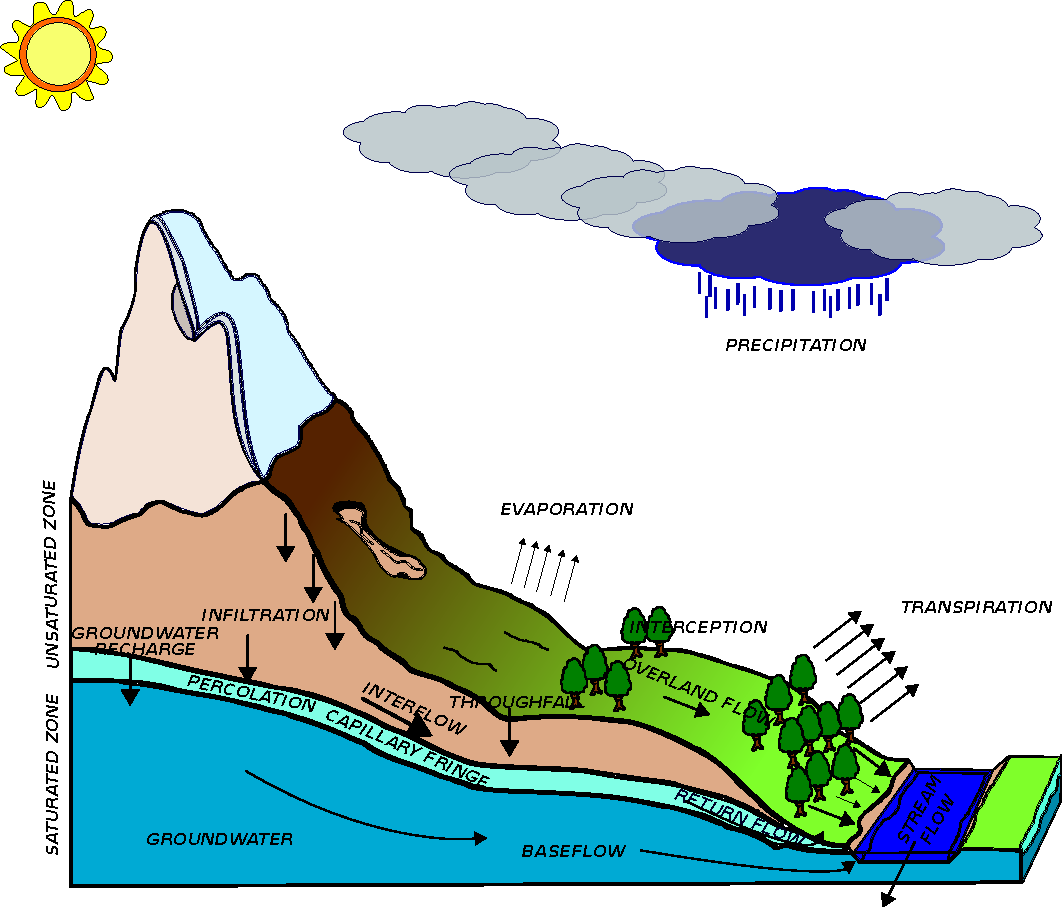
\includegraphics[width=1\textwidth]{./images/pic_general/bilancio}
    \textsl{\caption{The water cycle} \label{}}
  \end{minipage}
\end{center}
\end{figure}


Many hydrological models, commercial and research research oriented, allow to analyze the water and energy exchanges between the soil and the low atmosphere. However, often the models treat accurately only some aspects of the water cycle, i.e. the run-off or the boundary layer, and study the other parts in an approximate way.
GEOtop  \citep{Rigon06}, on the other hand, is a physically based distributed hydrological model that analyzes the complete water cycle in a catchment. The model is conceived to deal with complex topographies, as it provides each grid point of the domain with the topographical characteristics of the basin (elevation, slope, aspect, shadow, sky view factor). The soil/rock thermal and hydraulic characteristics are given in input in form of maps, together with a vertical description of the layers to account for heterogeneous stratigraphies. The vegetation and soil cover features may also be specified in form of maps.
The meteorological data, collected in one or more points in the catchment, are spatially distributed to each grid point thanks to the {\it Micromet} model \citep{liston2006meteorological}. 
Then the model calculates the energy and mass balance in the catchment through a 3D solver for Richards' equation \citep{EndrizziInvest2010} and a 1D solver for the energy equation \citep{dall2010energy}. 
The vegetation is treated according to a double layer scheme \citep{endrizzi2010observations}, that allows to separate the contribution of vegetation and of the surface on the turbulent fluxes.
The snow module, originally implemented with a monolayer scheme \citep{zanotti2004geotop}, now calculates accumulation and melting through a multilayer discretization of the snowpack \citep{endrizzi2007phd}. Recently the model has been enriched with a {\it blowing snow} module, based on \citet{pomeroy1993prairie} e \citet{essery1999distributed} contributions, that allows to account the accumulation and scour due to the wind action.
GEOtop represents a useful tool to simulate:
\begin{itemize}
\item the soil water content \citep{gebremichael2009scaling}
\item the evaporation of the soil \citep{Bertoldi2006, bertoldi2010topographical};
\item the transpiration of the vegetation \citep{endrizzi2010observations};
\item the snow in a catchment \citep{zanotti2004geotop, endrizzi2007phd, endrizzi2010observations, dallamico2011snow};
\item the surface temperature in a basin \citep{bertoldi2010topographical};
\item the temperature in the soil/rock also under freezing conditions \citep{dallamico2010phd};
\item the glacier mass balance \citep{NoldinNV2010};
\item the water table and thaw depth interactions \citep{EndrizziInvest2010};
\item and the water discharge in an outlet \citep{Rigon06}
\end{itemize}



\begin{figure}[!h]
\begin{center}
  \begin{minipage}[c]{.80\textwidth}
    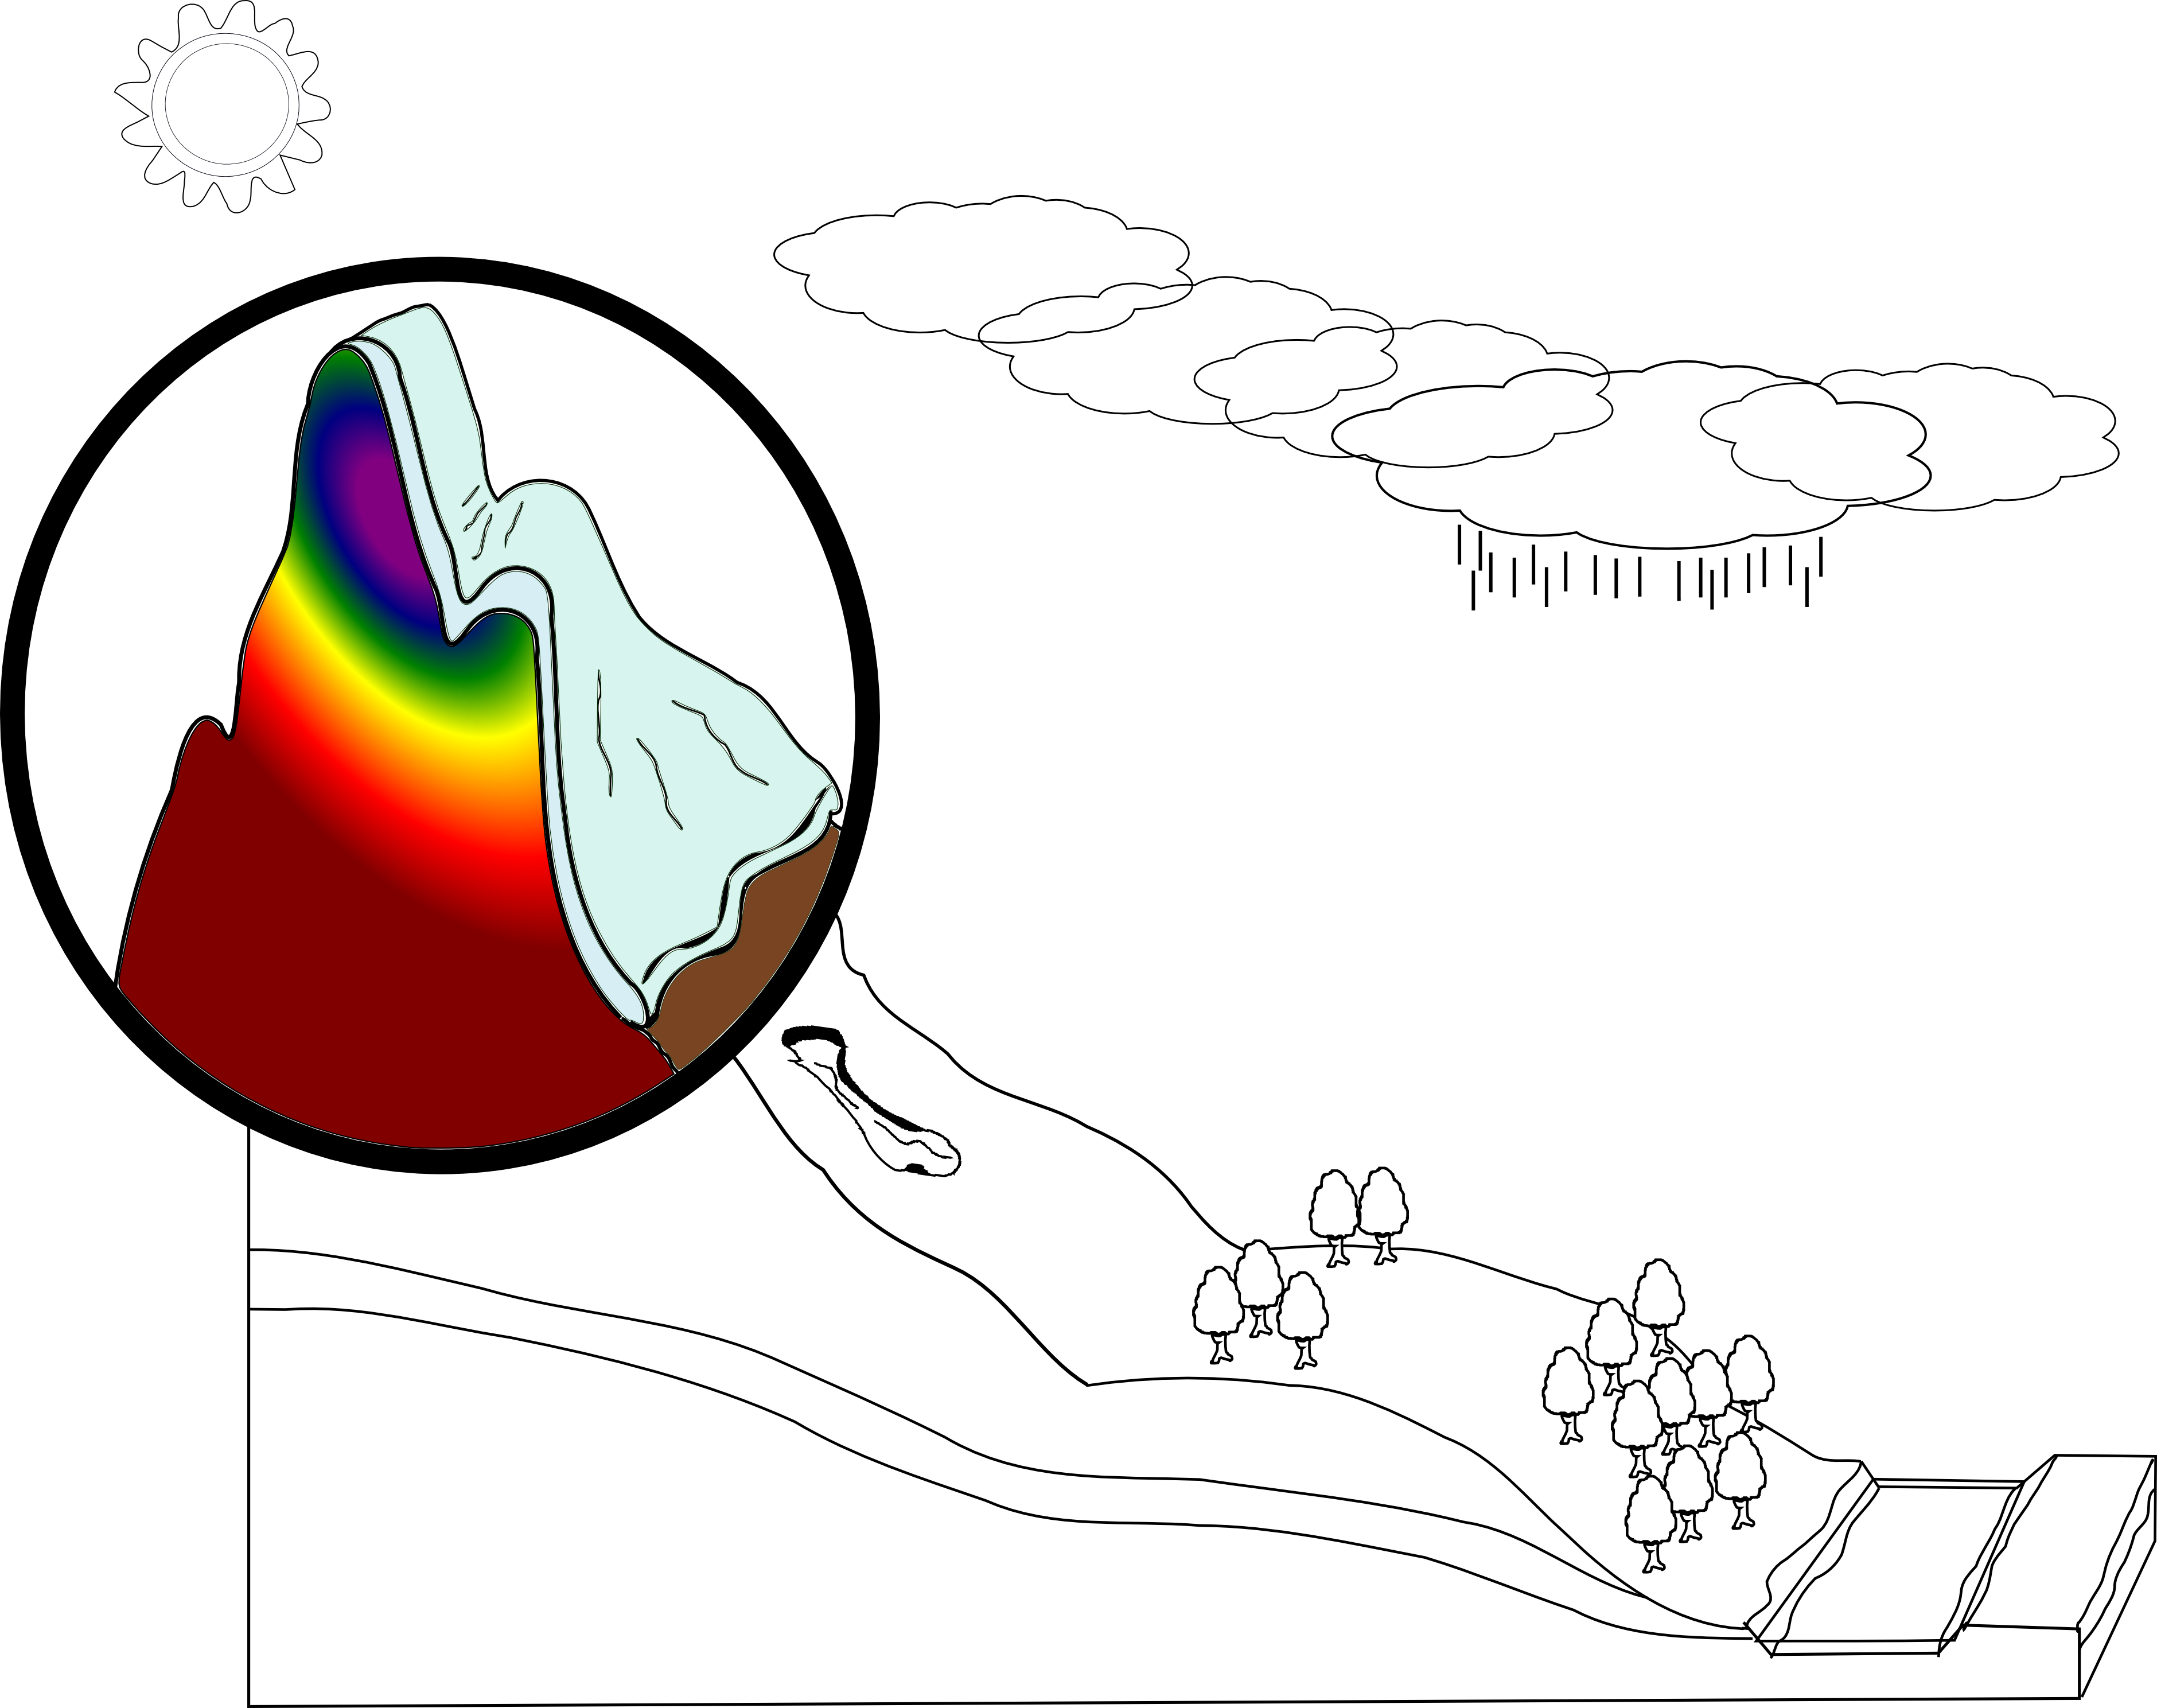
\includegraphics[width=0.7\textwidth]{./images/pic_template/criosfera_temp_grad.png}
    \textsl{\caption{Cryosphere: snow, glacier, permafrost} \label{}}
  \end{minipage}
\end{center}
\end{figure}



\begin{figure}[!h]
\begin{center}
  \begin{minipage}[c]{.80\textwidth}
    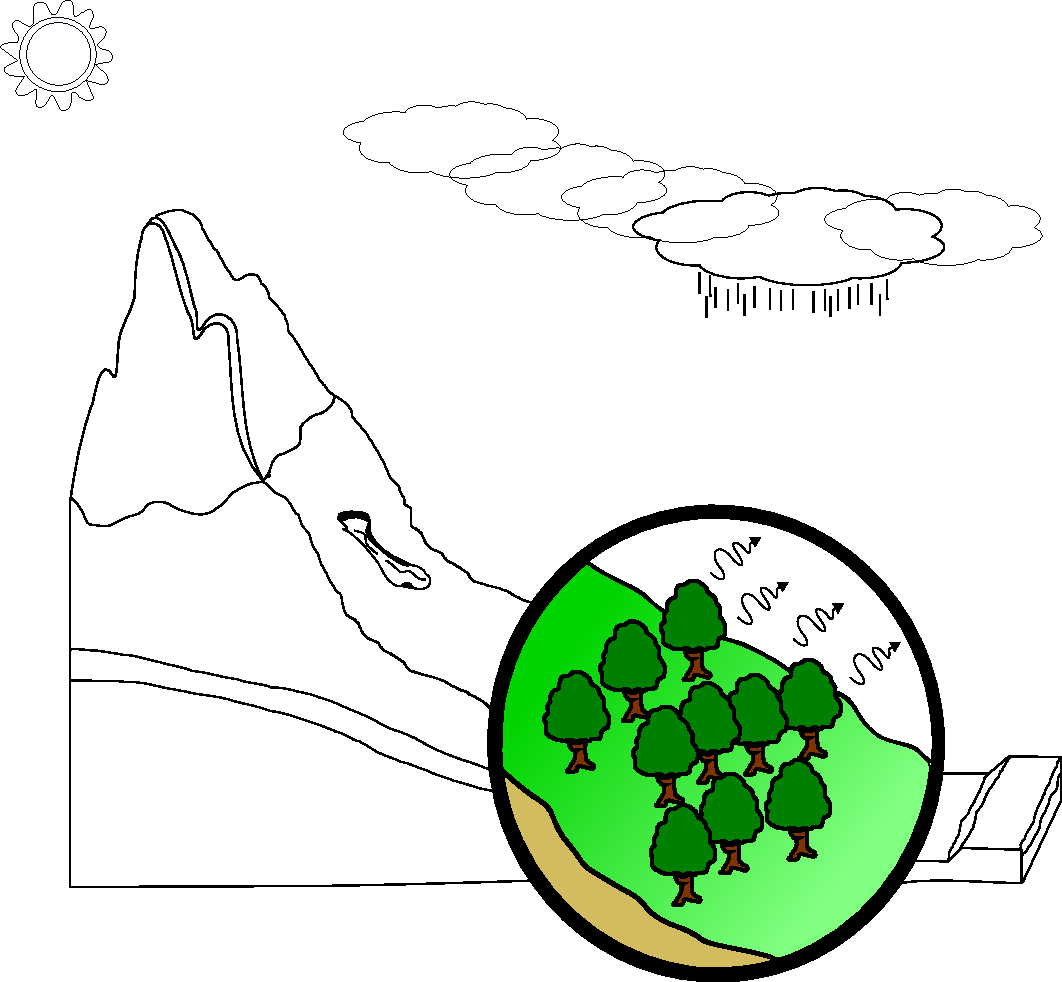
\includegraphics[width=0.7\textwidth]{./images/pic_template/vegetazione.pdf}
    \textsl{\caption{Vegetation and surface fluxes} \label{}}
  \end{minipage}
\end{center}
\end{figure}


\begin{figure}[!h]
\begin{center}
  \begin{minipage}[c]{.80\textwidth}
    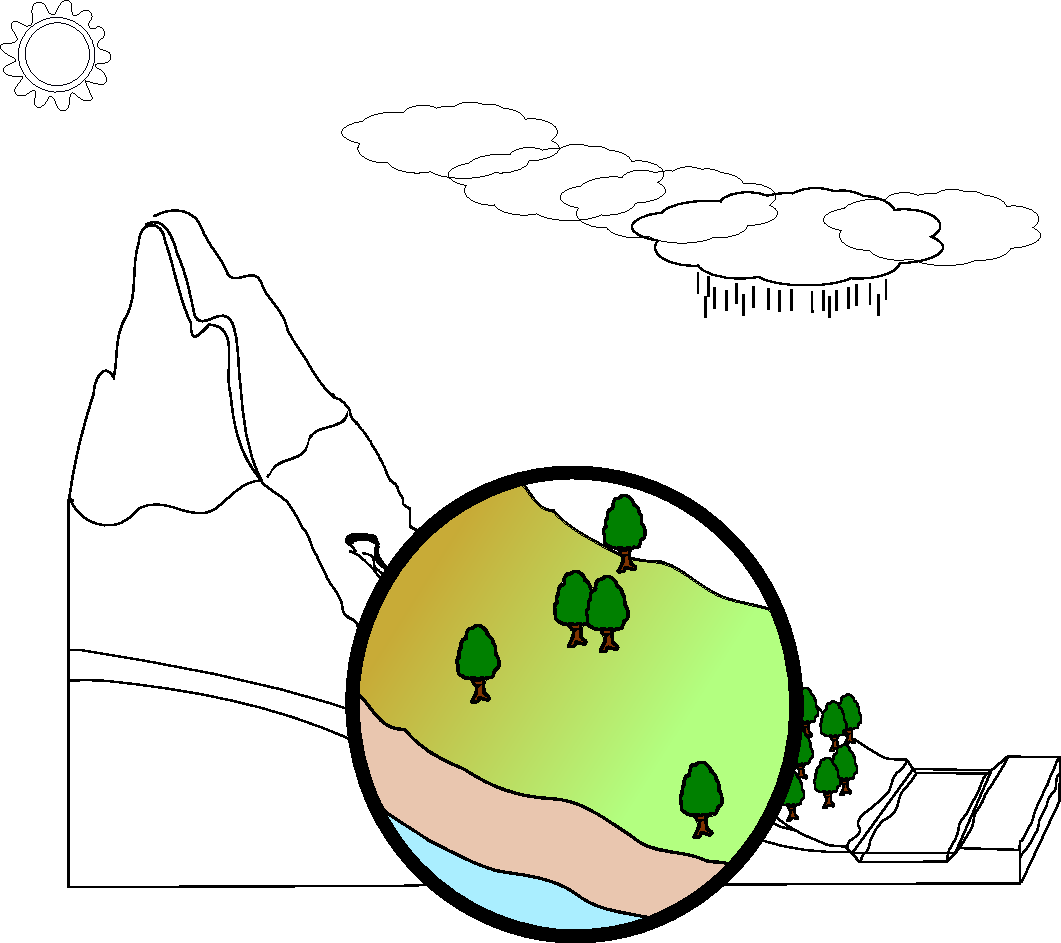
\includegraphics[width=0.7\textwidth]{./images/pic_template/suolo.pdf}
    \textsl{\caption{Soil: infiltration, water content, discharge} \label{}}
  \end{minipage}
\end{center}
\end{figure}


%\begin{figure}[!h]
%\begin{center}
%  \begin{minipage}[c]{.80\textwidth}
%    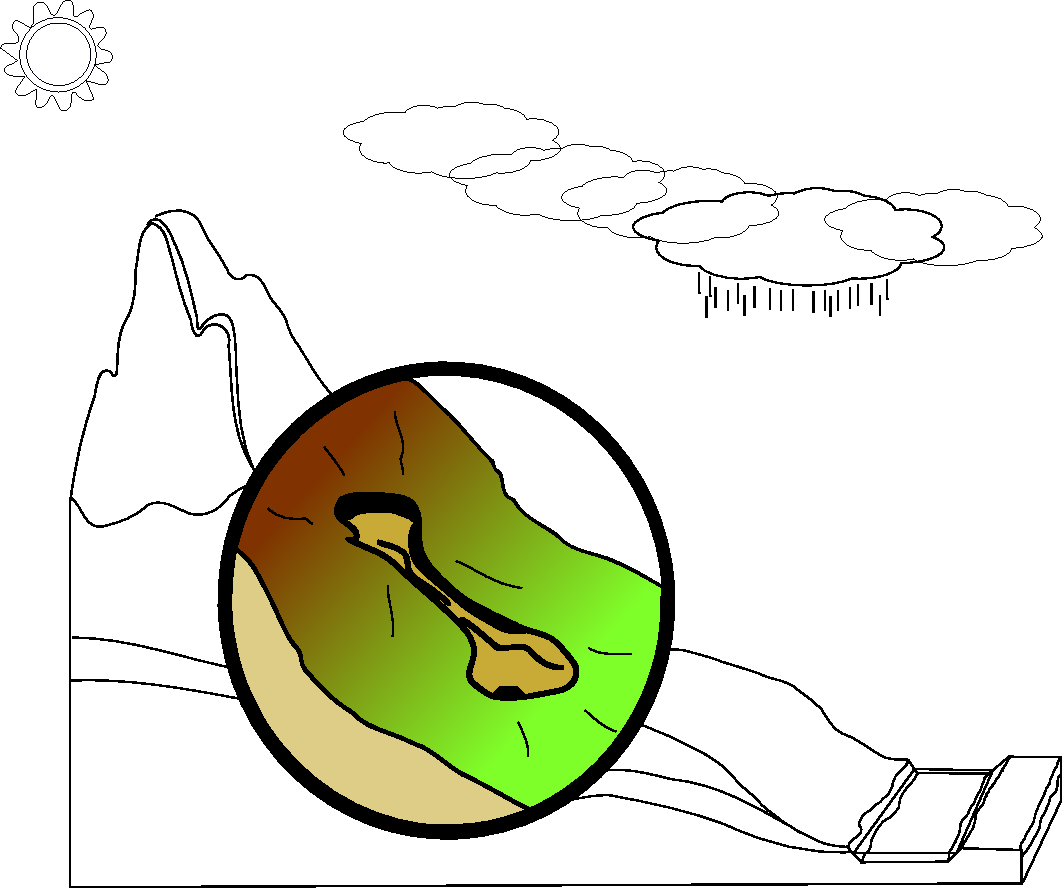
\includegraphics[width=1\textwidth]{./images/schemi/dissesti.pdf}
%    \textsl{\caption{Shallow landslides} \label{}}
%  \end{minipage}
%\end{center}
%\end{figure}
%
%\section{History}
%GEOtop concise history up to the first public release - by Riccardo Rigon
%
%``{\it As scientists we are intrigued by the possibility of assembling our knowledge into a neat package to show that we do, after all, understand our science and its complex interrelated phenomena.}'' (W.M., Kohler, 1969). 
%
%\subsection{GEOtop 0.5}
%The first version of GEOtop (0.5) was mostly financed by the Autonomous Province of Trento through the Serraia project and by the Italian Ministry of Research and University through the Cofin 1999 project.
%The very first step was due to the reading of the Entekhaby review of moddling the whole hydrological cycle [e.g. - Marani and Rigon (eds), 1997], and started with  the master thesis of Paolo Verardo and his subsequent work in 1998. Around a year was spent to implement a decent model for evapotranspiration in a complex terrain environment, according to the Penman-Monteith (PM) schematization, and all the necessary incoming radiation treatments.
% Especially the view angle and the shadowing routine were delicate to implement. The  problem of data assimilation and regionalization (at that time the only data we had were those coming from traditional hydro-meteorological stations and we do not have many of them) was face for the first time. 
%Apart from the geomorphological data that we extract from DEMs (the "sine qua non" basis of all the work) we had to regionalize: air-surface temperature (varying obviously with the elevation of the terrain), net radiation (that has to be first derived from that at the atmosphere top by the evaluation of an atmospheric thickness which has to be regionalized too) and wind speed. 
%In sequence it was decided decided to use: kriging  techniques and the hypothesis of adiabatic temperature profile (for air temperature); Brutsaert [1983] paper results (for atmosphere emissivity) and constant (or kriged) wind speed everywhere. 
%
%The heat conduction into the ground was parametrized as a linear combination of a sinusoidal function as Entekhaby suggested [1997] (this has been eventually changed). That work  was also inspired by the routines  of IPW (Image Processing Workbench) [Frew, 1990]. 
%Actually it was tried to get IPW working: but its pervasive scripting base (scripting is good but there is a point after which it makes the code organization unclear), the discontinued support and ignorance of IPW code internals, led  to built a new system from the scratch. 
%
%Despite of the approximations introduced, GEOtop 0.5 model worked fairly well in estimating the net longwave and shortwave radiation in any point across a basin and at any hour of the day, and could give also reliable estimates of the potential evapotranspiration on a daily basis. However to obtain the real evapotranspiration was a different question (and, obviously, to validate it, eve a different one).  
%Marco Pegoretti [1999] added to the evapotranspiration modules a rainfall-runoff model (temporary called GEOMODEL). The approach to the problem of rainfall-runoff  was strongly influenced by the work of Rodriguez-Iturbe and Valdes [1979] and Gupta et al [1980],  and I was reluctant to abandon the simplicity of a GIUH-based model in favor of a fully distributed model. 
%
%Of the many ideas behind the theory of the GIUH there is the observation that the river basin is a complex system (an interplay of hillslopes and channels) but, at least for the forecasting of floods, just a simple model works leading to the conclusion that dynamics works in simplifying  statistically the complexity and the heterogeneity underneath.
%
%The big problem in the GIUH approach however was (and is) the determination of the effective rainfall, i.e. the correct separation of surface runoff (interpreted as the cause of the flood surge) from subsurface flow (which must be actually treated separately and routed to the channels in a slower way), especially in dependence of storm events of diverse intensity, duration and inter-arrival time. 
%
%A model more or less contemporary to the GIUH is the TOPMODEL by Beven and Kirkby [1979]. It is based on the paradigm that runoff production is due to saturated areas (according to Dunne and Black, 1970). Thus, once one knows which areas are saturated and describes their growing during an event, the problem of the runoff coefficient is almost solved while routing of water to an outlet can be accomplished by some simple mechanism (the Muskingum-Cunge model at least in the original papers). 
%Thus, an idea could have been to merge the best of the two formulations, the GIUH concept with the TOPMODEL. However the hypothesis on which the TOPMODEL has been based, mainly the stationarity of the hillslope subsurface fluxes,  in one way simplifies the life of the modeler, but on the other is from many points of view a limitation which needs several work-around as described in  Beven et al., [2002]. In fact, when the final goal is not simply the production of a well-fitted flood wave, but for instance the estimation of local soil moisture contents, the TOPMODEL fails to be precise enough [e.g., Grayson and Wilson, 2002]. 
%
%Furthermore, the parameters entering the model become "effective'' parameters and lose their original physical significance (for instance, the hydraulic conductivity cannot be validated by local field measurements), and need to be "calibrated" ex-post. Other limitations will be mentioned below when talking about the GEOTP 0.875 version. In any case, the TOPMODEL concept has been demonstrated to be a good tool to model floods in small-to -medium catchments, and has been considered the reference hydrological model for many of the researchers during the '90s. The TOPMODEL's ability to forecast floods derives also from its account (trivial indeed) of the topology and geometry of small- catchment flow paths: it was shown, in fact, that in small watersheds (up to at least 1000 square kilometers), hillslope residence time dominates the characteristic time of flood formation and that topology and geometry of river basins are sufficient with very minimalist dynamics to explain the shape of floods [Rinaldo et al, 1991; Rigon et al, 1996, Rinaldo et al., 1995, D'Odorico, 1996; D'Odorico and Rigon, 2003]. 
%Thus, it was decided  to build completely new subsurface and surface models, still driven by gravity (i.e. by slope as the TOPMODEL and not by the total hydraulic head) but, as a first approximation to the final wishes, introducing the buffer to cope with infiltration into the vadose zone.  Subsurface flow was produced only by the saturated layer (including the capillary fringe), if present, and lateral surface runoff was routed as a kinematic wave (and through Manning/Gauckler-Strikler equation for velocities). 
%
%In doing this, it was searched  a better characterization of flow paths, with reference to the bedrock, instead of to the surface topography [see McDonnell et al., 1996]: this could be done by measuring soil depth or interpolating it for instance as in [Heimsath et al, 1997 or Roering et al, 1999; please see the overlooked  Bertoldi et al, 2006 for the details]. 
%
%In this separation of surface and subsurface fluxes, GEOtop 0.5 was similar to the grid bases THALES [Grayson et al., 1994a,1994b] or the more recent NEWTHALES. At first, the version of GEOtop by Verardo-Pregoretti-Rigon (GEOTOP 0.5) could work without an explicit channel routing assigning a locally variable roughness and hydraulic radius; usually, however, channels were determined by accurate topographic analysis and explicitly treated. Channels routing was performed by a GIUH theory as in Rinaldo et al [1995], where channel celerity and hydrodynamic dispersion were  considered spatially uniform and constant in time. 
%
%Instead of the effective rainfall, the spatially an temporally distributed input to channels was produced by GEOtop, i.e. the GEOMODEL produced patterns of spatially distributed soil moisture, and these patterns were used to reduce the potential evapotranspiration to its real counterpart as described in Bertoldi et al., [2002]. 
%
%\subsection{GEOtop 0.75}
%(mostly financed by COFIN 2001, THARMIT Eu Project, CUDAM - CofinLab 2001, ASI 54/2000)
%
%The use of PM  equation for evapotranspiration was indeed unsatisfactory from many points of view. For instance, it depends on air temperature that was derived from interpolation, and it was envisioned that  the parametrization of fluxes into the ground, sensitive both to the ground cover and to the water content, could be modeled directly, haven as a  result that many of the variables and parameters that were known to be correlated were actually treated separately.
% 
%Thus, with the Master thesis of Giacomo Bertoldi[2000] wit was decided throw away the PM equation (actually we kept it for comparison), and to solve directly the energy balance in any point of the basin. This was the birth of GEOTOP 0.75 which is thoroughly documented in Bertoldi et al[2002a,b] and Rigon et al [2002]. It was actually a SVAT model plus an rainfall-runoff model coupled together. GEOtop needed several parameters to be run, however the modeling could have been considered parsimonious, if all the prognostic capabilities were to be considered.   The user could switch-off the SVAT part and have a parametrically parsimonious rainfall-runoff model, or vice-versa she can switch-off the rainfall-runoff model and have a reasonably simple SVAT model. 
%Large efforts were  done in cleaning the old code and improving the input-outputs. Credits must be given to the work of Liang et al. [1994] with their work on VIC (which is however parametrized to work at much larger scales) and on Wigmosta et al. [1994] whose model is very similar to the version 0.75 of GEOtop (but was mostly a case of evolutionary convergence since the comparison came after the GEOtop implementation). 
%From the beginning,  the model was used  to forecast the whole hydrological cycle, even if a reasonable snow modeling still had to arrive. We were looking also to other topics. 
% Eco-hydrology was, in fact, a research thread whose seeds where already in Rodriguez-Iturbe's mind when I was working with him at the Texas A\&M University (1994-1996) and of which I was concerned from the beginning of the project. 
%
%Ecohydrology [Rodriguez-Iturbe, 2000] has roots in the work of Eagleson [1978, 2003], Phili, Brutsaert, Hillel [1990],s and others and is one of the hot issues in these hydrological decades [Rodriguez-Iturbe, 2000]. 
%
%For validation of the modules, a key role in this had Tom Over who, besides giving a lot of suggestions making the concepts behind the model clear, suggested to use the South Great Planes 97 experiment data set, thing that we promptly did as it appears in the first journal paper about the model Rigon et al., 2006). 
%
%Based partially on GEOtop 0.75 (and on the subsequent GEOtop 0.875) came all the work by Reza Entezarolmahdi who tried first to create an automatic calibration system for the model. This actually used MOSC-EM [CITATIONS] which, however was never really integrated in the model.  The work of Reza was really interesting for many point of view, but probably a little advanced with respect to times and finished to a dead-end from which we hope to resume it sometimes in the very next future. 
%
%\subsection{GEOtop 0.875}
%(mostly financed by TIDE EU Project, CUDAM Cofinlab COFIN 2001, THARMIT EU project)
%
%This version finally contained a snow accumulation and melt model (derived by the Utah Energy Balance -UEB- by Tarboton and Luce, [1992]) implemented by Fabrizio Zanotti [2003] with the help of Giacomo Bertoldi .  It also included a post-processor, the S-FACTOR , which performed a landslide and debris-flow triggering implemented by Christian Tiso [2003] (eventually evaluated into GEOtop-SF by Silvia Simoni).  Both the implementations were the outcome of two M.S. thesis.  Snow-melting and soil freezing are essential components in the hydrological cycle of mountain catchments and cannot not be overlooked. Landslide and debris-flow triggering are also an issue with particular relevance in mountains areas, such that floods in mountain areas are usually the combined effect of large liquid and solid discharges whose effects cannot be separated: GEOtop with this version started to a tool for studying these phenomena. 
%
%However, with the version 0.875, we wanted to attack the problem of a sound hillslope-hydrology modeling. 
%
%So far, our understanding of mountain catchments in fact was based on hillslope hydrology, as reviewed for instance in Wipkey and Kirkby [1978], and  the "perceptual" hillslope model that we had at that time derived from the assumption that it was possible to neglect the transients in the water fluxes [in the sense clarified in Iverson, 2000]; that topographic gradients dominate the hydrologic response; that hydraulic conductivity strongly decreases with depth in the soil and, not independently, that runoff occurs mostly owing to saturation excess. 
%This last assumption in turn was  based upon the results of a long series of experiments from the late seventies on by American geomormologists (Dunne, Black, Dietrich, Montgomery, Torres), and was supported by many others (among these: Moore, Grayson, Sivapalan, Wood). 
%These experiments and subsequent research activities changed the belief spread by Horton that runoff was mostly due to the infiltration excess mechanism. Developing hydrological models based on saturation excess ideas (which involved further simplification) originated a series of rainfall-runoff models among which the already cited TOPMODEL [Beven and Kirkby,1979; Sivapalan et al, 1991; Franchini et al, 1996] is the most successful product. 
% 
%There are many aspects that could be improved with respect with that model. For instance,  in characterizing  the subsurface flow field more in terms of total head, even if in simplified form as in Iverson [2000], than in terms of the topographic gradient, as a first step toward the integration of the three dimensional Richards equation. These  steps were implemented by the master thesis of Davide Tamanini [2003] that made GEOtop able to simulate transient subsurface flow, and both saturation excess and infiltration excess runoff.  A first parameterization of the soil water retention curves was also implemented in the model. It is this code that was used in the first journal papers on GEOtop (Zanotti et al., 2004, Rigon et al., 2006, Bertoldi et al., 2006). Upon this code was based the work by Silvia Simoni, helped by Fabrizio Zanotti which produced the GEOtop-SF postprocessor that was able to estimate statistics of the stability of a hillslope. This work, in turn, produced Simoni Ph.D. thesis  and Simoni et al., [2008]. 
%
%In GEOtop 0.875 the integration of Richards equation followed a custom numerical scheme that was exceedingly complicate and non standard. Moreover, the integration scheme was not fully 3D, but could have been defined 2D + 1D, where "2D" stands for the lateral flow, obtained by using the Darcy Buckingham law, and 1D was the resolution of a one dimensional Richards equation. Despite these limitations, we could obtain reasonable reproduction of soil moisture distributions,  good discharges at the outlet of basins, excellent reproduction of summer soil temperatures, and what we considered a good reproduction of turbulent heat and evapotranspiration exchanges. 
%
%
%\subsection{GEOtop 0.9375}
% and subsequent version till the first public release
%(mainly financed by Projects with Servizio geologico PAT, progetto MORFEO by ASI, and EU IRASMOS and  AQUATERRA projects)
%
%The new development started with in mind that we had sooner or later to switch to a version of GEOtop with a full 3D integration of Richards equation. 
%
%However, the first new improvement of GEOtop was in the direction to include a multiple layer  modeling of snow and a first core of the freezing soil subroutines.  This was mainly accomplished during the Ph.S thesis of Stefano Endrizzi [2007], and greatly improved in his subsequent work at Saskatoon, working with Phil Marsh and Bill Quinton, and recently at Zurich University collaborating with  Stephan Gruber. 
%
%Why complicating even more an already complex model? Moreover, why getting a new snow model, if the Utah energy balance seemed to work fine, as written in Zanotti et al., 2004?
%The rational behind this choice was essentially that the snow water equivalent was not enough for comparing snow measurement in the field with model outcomes. Clearly snow water equivalent (SWE) was enough just for those willing to cope with total water volume generated after snow melting, but not sufficient for studying and understanding the processes behind snowpack evolution and ablation. Nor even for having a reasonable estimate of soil temperature under the snow, and other interesting prognostics, like snow density. 
%
%However, Stefano's efforts were not limited to snow. He worked hard, for getting a consistent integrator of Richards equation, that he based on a Newton Krilov-method (Kelley, 2003).  Besides he decided to change the surface water flow  equation and numerics, by using the shallow water equation integrated with a robust but explicit method.  This resulted in a very stable and reliable code that constitutes the core of the first public version of GEOtop. In fact Stefano decided to move from the the fraction of geometric series of  $\sum_i (1/2)^i$ to the integer 1.
%
%The collaboration of Stefano and Matteo Dall'Amico produced also a consistent integrator of the freezing soil moisture, after that Matteo, in his Ph.D thesis disentangled, at least for ourselves,  a lot of thermodynamics (and together, we introduced a simple, and "normal" thermodynamic notation). This work has been documented in Dall'Amico et al., 2010 LINK, and produced a paper for The Cryosphere LINK. 
%
%\subsection{Stefano Endrizzi's work}
%
%Up to version 0.875 version GEOtop was pretty much a home made effort, mainly pursued by Master and Ph.D students of Trento University. However, since then, either because the Ph.D students became doctors and spread around, and because other discovered the potential our work, GEOtop started to became really internationally used. Han Xunjun in China used GEOtop in his data assimilation system implementing an ensemble Kalman filter (in Python). The Lausanne group under the direction of Marc Parlange, within the collaboration of Silvia Simoni, and the direct coding efforts of Thomas Egger implemented a real time version of the model that is giving its results everyday (http://lsir-hydrosys01.epfl.ch:22006/). John Albertson and his group implemented an erosion module to be coupled with GEOtop. In Trento, a version of GEOtop, called GEOtop-EO implemented a prototype of  infrastructure that includes besides the modeling core, a geographical database, with a raster service (built upon RAMADDA -LINK) and a visualization system based on JGrass. This was done for the project MORFEO (LINK).  At Bolzano, in EURAC, Giacomo Bertoldi and Stefano Dallachiesa, endowed GEOtop with an external (so far) vegetation dynamical model (itself came from previous work by Albertson and Montaldo). Last, but not least, Mountain-eering made of GEOtop the center of its business plan, and supported the completion of the freezing soil module, and is going to develop a new NetCDF input/output system, and the creation of some data assimilation of snow measures. 
%
%Credits to work of the group of Lousanne should be given to have also included in GEOtop the METEO/IO environment which was the way to link the model to a real-time acquisition system.  Stefano Endrizzi himself, when at Saskatoon, discovered the work of Liston and Elder [2006] with MICROMET, and included it in the GEOtop distribution with the permission of the Authors. 
%
%Also other player came  to the game. Arpa Val D'Aosta decided to make of GEOtop the principal tool for doing analysis on snow and permafrost, and it is going to support its improvement and usability. The Karlshrue Institute of Technology in Garmisch-Partenkirchen (and particularly Prof. Harald Kunstmann, and coworkers) adopted for simulation for one of their TERENO experiment (LINK).  
%
%This, just to mention partial developments, not all of them yet flowed into the main version of the model. All of these efforts, in fact, could not being really unified in a single product. 
%
%\subsection{GEOtop in Zurich}
%
%
%\subsection{Future perspectives}
%So
%
%So the questions for the future are: 
%
%how can we manage the future of this international crew, letting any single her freedom ?
%and making the whole community grow cooperatively ?
%how giving anyone the proper credits which are necessary to go ahead ?
%how maintain while moving on relevant pieces of software still available avoiding to wipe them out (as it happens for the PM coed, and more recently, with the former runoff-modules. to do a couple of examples ?
%
%I gave already some possible direction (see for instance LINK) that derives from the issue raised by the work of Stefano Endrizzi and Hydrologis, and in an effort to unify all of my previous work lines.
%
%However, this is not an aster I want to do by myself. The community around GEOtop must give its opinion. Because the only perfect model is the evolving one, since many contenders appear, our knowledge grows, and all of us work hard. 
%
%Relevant Literature 

%%%%%%%%%%%%%%%%%%%%%%%%%%%%%%%%%%%%%%%%%%%%%%%%%%%%%%%%%%%%%%%
\chapter{Compiling Instructions}\label{chap:User Manual}
%%%%%%%%%%%%%%%%%%%%%%%%%%%%%%%%%%%%%%%%%%%%%%%%%%%%%%%%%%%%%%%

\noindent Before you begin to use GEOtop, is advisable you subscribe to the
users mailing list. By doing it you will receive informations by developers and
other users, and you will be able to post your question to the community as
well. Follow the instruction at the following link:\\

\textcolor{blue}{\underline{{https://groups.google.com/forum/?pli=1\#!forum/geotopusers}}}\\


\noindent GEOtop runs properly under:
\begin{itemize}
 \item Linux platform;
 \item Mac platform;
 \item Windows platform.
\end{itemize}


If you want to build GEOtop from sources in your own machine (Linux and MacOSX):

see here: 

\textcolor{blue}{\underline{{https://github.com/geotopmodel/geotop/blob/master/doc/Install.rst}}}\\

If you prefer to install GEOtop via Docker to avoid manual installation of packages:

see here: 

\textcolor{blue}{\underline{{https://hub.docker.com/r/omslab/geotop}}}\\


%%%%%%%%%%%%%%%%%%%%%%%%%%%%%%%%%%%%%%%%%%%%%%%%%%%%%%%%%%%%%%%
%\section{Compile GEOtop through a makefile}
%%%%%%%%%%%%%%%%%%%%%%%%%%%%%%%%%%%%%%%%%%%%%%%%%%%%%%%%%%%%%%%
%The GEOtop source code can be downloaded through a terminal (or command prompt if you are using Windows) by typing, 
%as shown in \textsl{Figure \ref{cmp}}:\\

%\textsl{"svn co https://dev.fsc.bz.it/repos/geotop/trunk/0.9375KMacKenzie"}\\
%\begin{figure}[!h]
%\begin{center}
%  \begin{minipage}[c]{.80\textwidth}
%    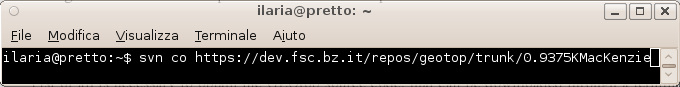
\includegraphics[width=1\textwidth]{./images/pic_compile/compile.png}
%    \textsl{\caption{Download GEOtop source code through a terminal} \label{cmp}}
%  \end{minipage}
%\end{center}
%\end{figure}


%\noindent The downloaded folder contains the folders:
%\begin{itemize}
% \item Debug: which contains the object file created during the compilation and the makefile
% \item geotop: which contains the code
% \item Libraries: which contains the support libraries
%\end{itemize}



%\footnotesize{
%\begin{verbatim}
%HM	= .
%LHM		= $(HM)
%BINPATH 	= $(LHM)/
%NAME		= geotop0.9375
%BINS		= $(BINPATH)/$(NAME)

%SCRSPATH1	= $(HM)/KMacKenzie
%LIBPATH1	= $(HM)/LIBRARIES/FLUIDTURTLES
%LIBPATH2	= $(HM)/LIBRARIES/ASCII
%LIBPATH3	= $(HM)/LIBRARIES/GEOMORPHOLOGYLIB
%LIBPATH4	= $(HM)/LIBRARIES/MATH2
%LIBPATH6	= $(HM)/LIBRARIES/KeyPalette
%LIBPATH7	= $(HM)/EXTERN

%OBJ		= 	$(SCRSPATH1)/energy.balance.o $(SCRSPATH1)/frost_table.o\
%		  	$(SCRSPATH1)/geotop.09375.o $(SCRSPATH1)/recovery.o\
%		  	$(SCRSPATH1)/input.09375.o $(SCRSPATH1)/meteo.09375.o\
%		  	$(SCRSPATH1)/output.09375.o $(SCRSPATH1)/pedo.funct.o\
%			$(SCRSPATH1)/radiation.o\
%			$(SCRSPATH1)/snow.09375.o $(SCRSPATH1)/times.o\
%			$(SCRSPATH1)/water.balance_1D.o $(SCRSPATH1)/turbulence.o\
%			$(SCRSPATH1)/water.balance_3D.o $(SCRSPATH1)/vegetation.o\
%			$(LIBPATH1)/alloc.o $(LIBPATH1)/error.o\
%			$(LIBPATH1)/list.o $(LIBPATH1)/t_io.o\
%			$(LIBPATH1)/tensors3D.o  $(LIBPATH1)/utilities.o\
%			$(LIBPATH1)/datamanipulation.o $(LIBPATH1)/random.o\
%			$(LIBPATH1)/linearalgebra.o $(LIBPATH1)/write_dem.o\
%			$(LIBPATH2)/import_ascii.o $(LIBPATH2)/rw_maps.o\
%			$(LIBPATH2)/write_ascii.o $(LIBPATH2)/tabs.o\
%			$(LIBPATH3)/networks.o $(LIBPATH3)/geomorphology.0875.o\
%			$(LIBPATH3)/shadows.o  $(LIBPATH3)/dtm_resolution.o\
%			$(LIBPATH4)/geo_statistic.09375.o $(LIBPATH4)/sparse_matrix.o\
%			$(LIBPATH4)/util_math.o\
%			$(LIBPATH6)/key.palette.o $(LIBPATH6)/get_filenames.o\
%			$(LIBPATH6)/additional_read_functions.o $(LIBPATH6)/read_command_line.o\
%			$(LIBPATH7)/PBSM.o $(LIBPATH7)/micromet.o

%HPATH1 	= $(LIBPATH1)
%HPATH2	= $(LIBPATH2)
%HPATH3  = $(LIBPATH3)
%HPATH4  = $(LIBPATH4)
%HPATH6  = $(LIBPATH6)
%HPATH7  = $(LIBPATH7)
%HPATH0  = $(SCRSPATH1)

%CFLAGS	= -O3 -g 
%INCLUDE = -I$(HPATH1) -I$(HPATH2) -I$(HPATH3) -I$(HPATH4)  -I$(HPATH6) -I$(HPATH7) -I$(HPATH0)

%DEBUG   = -g -Wall
%CC	= gcc $(DEBUG)
%CPP	= g++

%.cc.o: $*.cc $*.h
%	$(CPP) $(CPPFLAGS) -c $< $(INCLUDE) -o $@

%.c.o: $*.c $*.h
%	$(CC) $(CFLAGS) -c $< $(INCLUDE) -o $@

%
%all: geotop

%geotop: $(OBJ)
%	$(CC) -o $(BINS) $(OBJ) -lm -rdynamic -ldl -lstdc++ 
%clean:
%	rm -rf *.o *~ $(OBJ)
%\end{verbatim}
%}
%
%\noindent Open a terminal, go into the folder \textsl{Debug} by typing:
%
%\footnotesize{
%\begin{verbatim}
%$ cd Debug
%\end{verbatim}
%}


%By typing \textsl{"ls"} you should have the following files and folders \textsl{Figure \ref{fo}}:
%\begin{figure}[!h]
%\begin{center}
%  \begin{minipage}[c]{.80\textwidth}
%    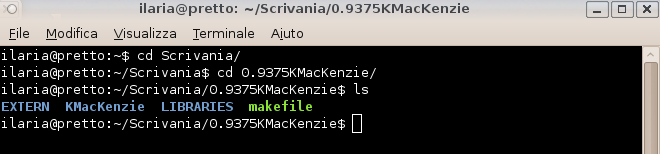
\includegraphics[width=1\textwidth]{./images/pic_compile/folders.png}
%    \textsl{\caption{Necessary files and folders to compile GEOtop through terminal} \label{fo}}
%  \end{minipage}
%\end{center}
%\end{figure}
%
%\noindent To compile GEOtop, type:
%
%\footnotesize{
%\begin{verbatim}
%$ make all
%\end{verbatim}
%}
%
%\noindent The executable file {\it GEOtop1.2} is now created in the {\it Debug} folder.

%\textsl{Figure \ref{fo_c}}.\\
%\begin{figure}[!h]
%\begin{center}
%  \begin{minipage}[c]{.80\textwidth}
%    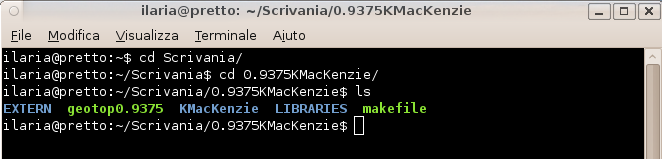
\includegraphics[width=1\textwidth]{./images/pic_compile/folders_compiled.png}
%    \textsl{\caption{Screenshot of the 0.9375KMackenzie folder with the executable} \label{fo_c}}
%  \end{minipage}
%\end{center}
%\end{figure}


%%%%%%%%%%%%%%%%%%%%%%%%%%%%%%%%%%%%%%%%%%%%%%%%%%%%%%%%%%%%%%%%
%\section{Compile and browse GEOtop through Eclipse}
%%%%%%%%%%%%%%%%%%%%%%%%%%%%%%%%%%%%%%%%%%%%%%%%%%%%%%%%%%%%%%%%
%Eclipse is a platform to build integrated development environments (IDEs).
%You first need to download and install it to succesfully compile 
%and browse GEOtop.\\

%\noindent For a complete tutorial download the presentation from:\\

%\textcolor{blue}{\underline{\textsl{http://www.geotop.org/cgi-bin/moin.cgi/Compile\_Instructions}{secondo}}}\\

%\noindent Download and extract the appropriate version for your operative
%system from the following link:\\

%\textcolor{blue}{\underline{\textsl{http://www.eclipse.org/downloads/}{terzo}}}

%
%%=============================================================%
%\subsection{Linux}
%%=============================================================%
%Using Linux Ubunt Karmic Koala 9.10, the Eclipse Galileo release has a bug with the Graphical Interface.
%To fix it follow this instrusctions:\\
%Supposing that the executable file is \textsl{"home\/ilaria\/Scrivania\/eclipse\_folder"},
%create a text file with the following string:\\
%\begin{center}
%  \begin{minipage}[c]{.4\textwidth}
%    \centering
%    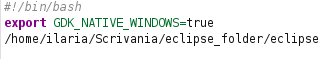
\includegraphics[width=1\textwidth]{./images/pic_compile/0_bug_fix.png}
%  \end{minipage}
%\end{center}
%Save it with a name that you like, but with the extension \textsl{".sh"} in the
%folder where the eclipse executable is, in this example \textsl{"home\/ilaria\/Scrivania\/eclipse\_folder"}.\\
%Right click on the file and allow it to be executable.\\
%Now lunch the .sh file instead of launching the eclipse icon and the bug is
%fixed\\

%%%%%%%%%%%%%%%%%%%%%%%%%%%%%%%%%%%%%%%%%%%%%%%%%%%%%%%%%%%%%%%%
%\subsection{CDT and SVN packages}
%%%%%%%%%%%%%%%%%%%%%%%%%%%%%%%%%%%%%%%%%%%%%%%%%%%%%%%%%%%%%%%%
%You now need to install two packages to succesfully compile GEOtop:
%\begin{itemize}
% \item CDT packages for eclipse Galileo: C/C++ Development Tooling
% \item SVN packages for eclipse Galileo
%\end{itemize}

%\paragraph{CDT packages:}
%\noindent To install the CDT packages go on: \textsl{"Help $\rightarrow$ Install New Software"}
%and in \textsl{"Work with"} add the repository \textsl{"http://download.eclipse.org/releases/galileo"}
%as shown in \textsl{Figure \ref{f:1}}\\
%\begin{figure}[!h]
%\begin{center}
%  \begin{minipage}[c]{.8\textwidth}
%    \centering
%    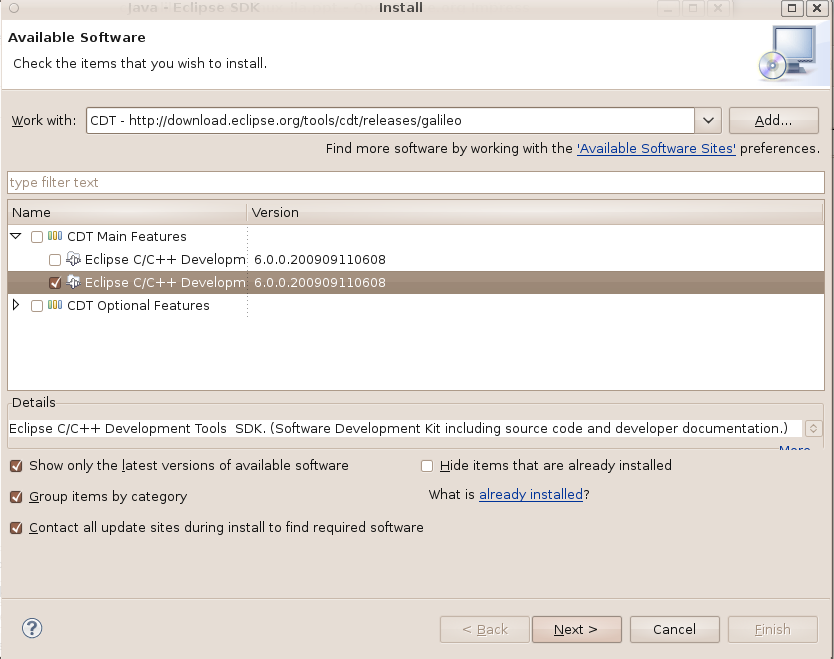
\includegraphics[width=1\textwidth]{./images/pic_compile/2_0_1_update.png}
%    \textsl{\caption{CDT} \label{f:1}}
%  \end{minipage}
%\end{center}
%\end{figure}

%\noindent Click on \textsl{"Next"}. Figure \textsl{\ref{f:2}} shows the packages you 
%are about to install and the license agreement, that you must accept.

%\begin{figure}[!h]
%\begin{center}
%  \begin{minipage}[c]{.45\textwidth}
%    \centering
%    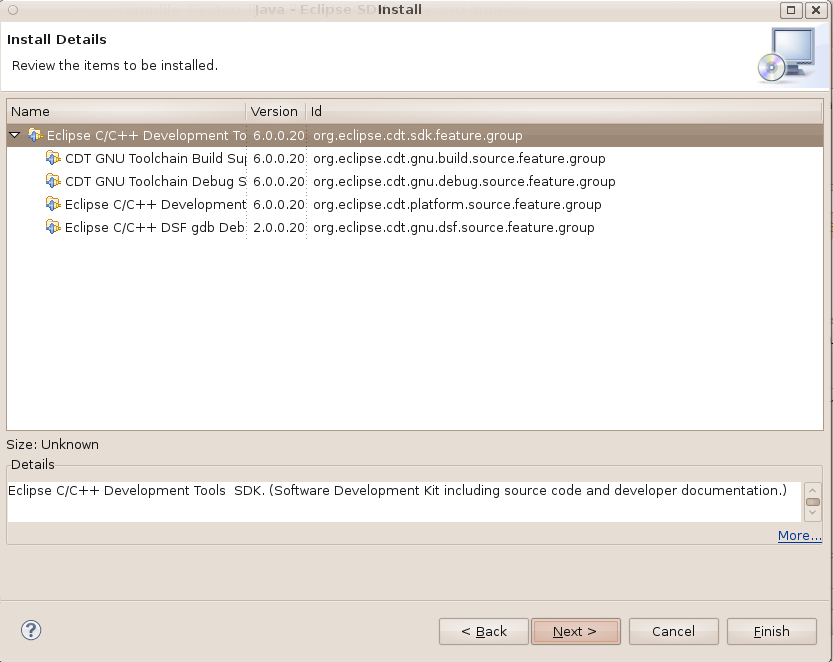
\includegraphics[width=1\textwidth]{./images/pic_compile/2_1_update.png}
%  \end{minipage}
%  \begin{minipage}[c]{.45\textwidth}
%    \centering
%    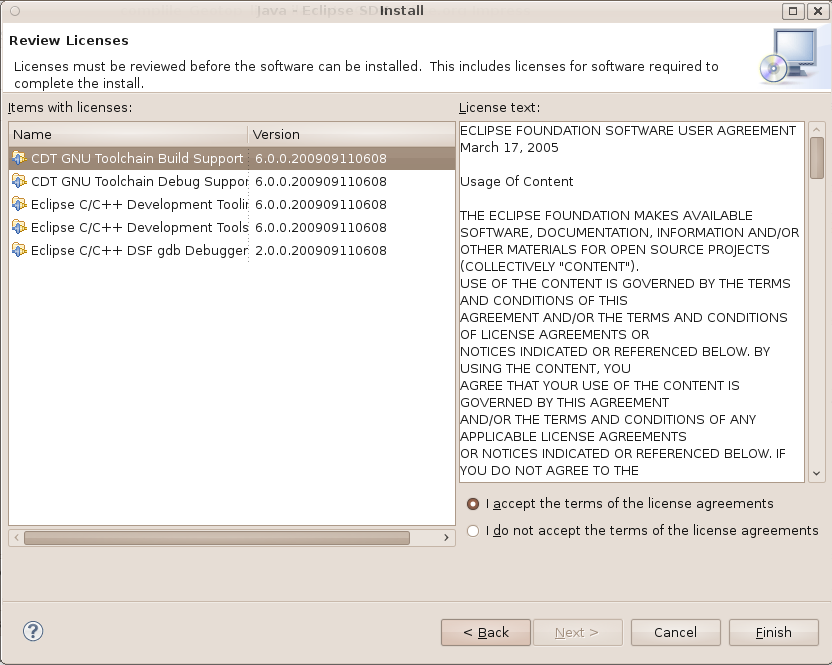
\includegraphics[width=1\textwidth]{./images/pic_compile/2_2_update.png}
%  \end{minipage}
%\end{center}
%    \textsl{\caption{CDT packages and License agreement} \label{f:2}}
%\end{figure}

%%%%%%%%%%%%%%%%%%%%%%%%%%%%%%%%%%%%%%%%%%%%%%%%%%%
%%%%%%%%%%%%%%%%%%%%%%%%%%%%%%%%%%%%%%%%%%%%%%%%%%%
%%%%%%%%%%%%%%%%%%%%%%%%%%%%%%%%%%%%%%%%%%%%%%%%%%%
%\newpage
%\paragraph{SVN packages:}
%\noindent To install the SVN packages go on:
%\begin{itemize}
% \item \textsl{"Help $\rightarrow$ Install New Software"}
%and in \textsl{"Work with"} add the repository \textsl{"http://download.eclipse.org/releases/galileo"}
%check the box \textsl{"Collaboration"} $\rightarrow$ \textsl{"Subversive SVN Team Provider (Incubator)"}
%as shown in \textsl{Figure\ref{f:3}}
% \item \noindent\textsl{"Help $\rightarrow$ Install New Software"}
%and in \textsl{"Work with"} add the repository \textsl{"http://www.polarion.org/projects/subversive/download/eclipse/2.0/update-site"}
%and then choose \textsl{"Subversive SVN Connectors"} $\rightarrow$ \textsl{"SVNKit Implementation (Optional)"}
%as shown in \textsl{Figure \ref{f:3_1}}
%\end{itemize}
% 

%\begin{figure}[!h]
%\begin{center}
%  \begin{minipage}[c]{.45\textwidth}
%    \centering
%    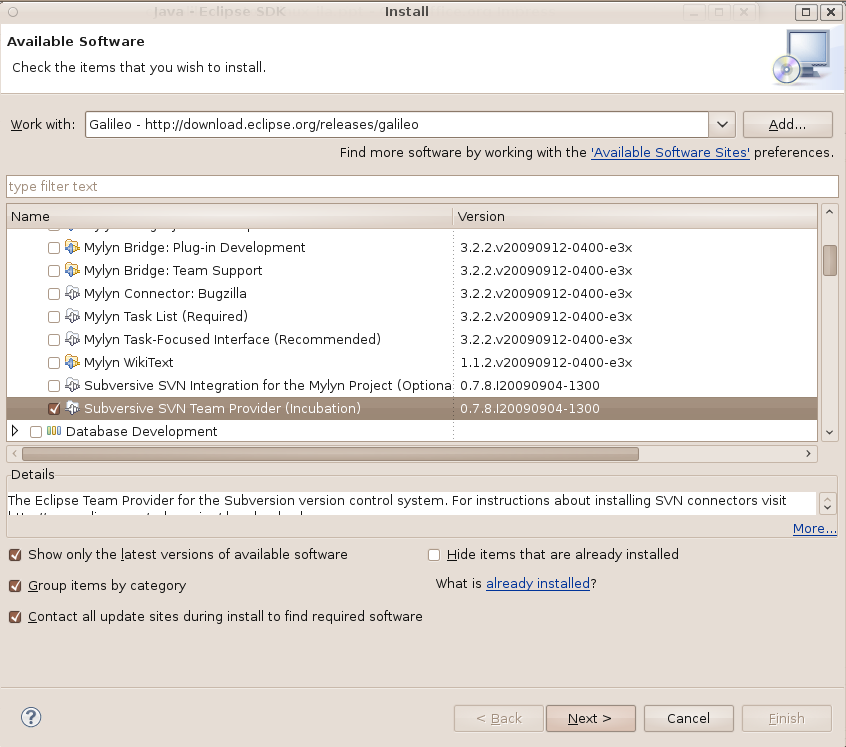
\includegraphics[width=1\textwidth]{./images/pic_compile/3_svn_1.png}
%  \end{minipage}
%%  \begin{minipage}[c]{.45\textwidth}
%%    \centering
%%    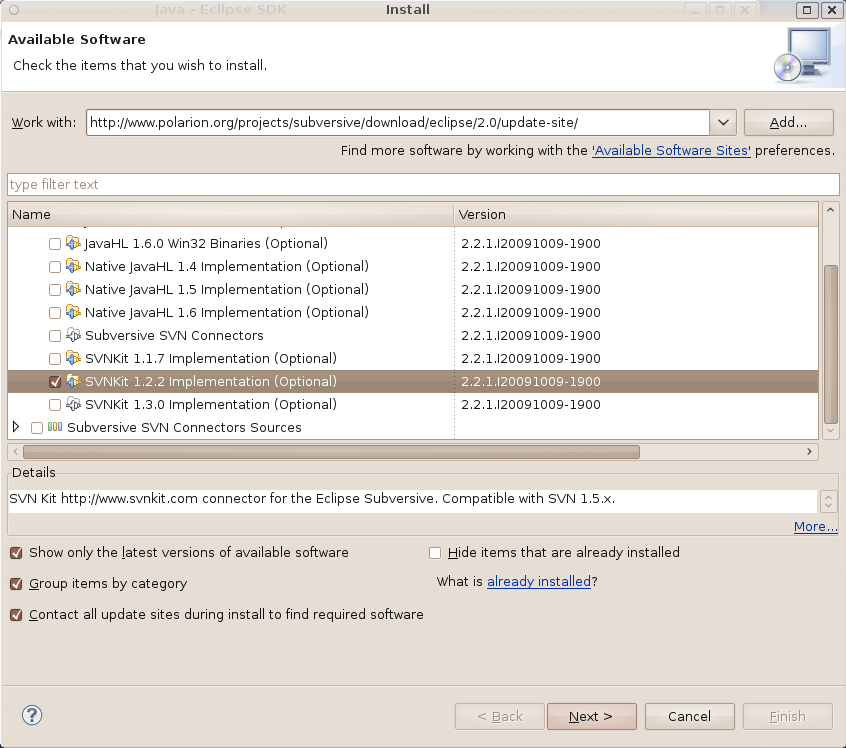
\includegraphics[width=1\textwidth]{./images/pic_compile/3_svn_2.png}
%%  \end{minipage}
%  \end{center}
%    \textsl{\caption{SVN} \label{f:3}}
%\end{figure}

%
%\begin{figure}[!h]
%\begin{center}
%  \begin{minipage}[c]{.45\textwidth}
%    \centering
%    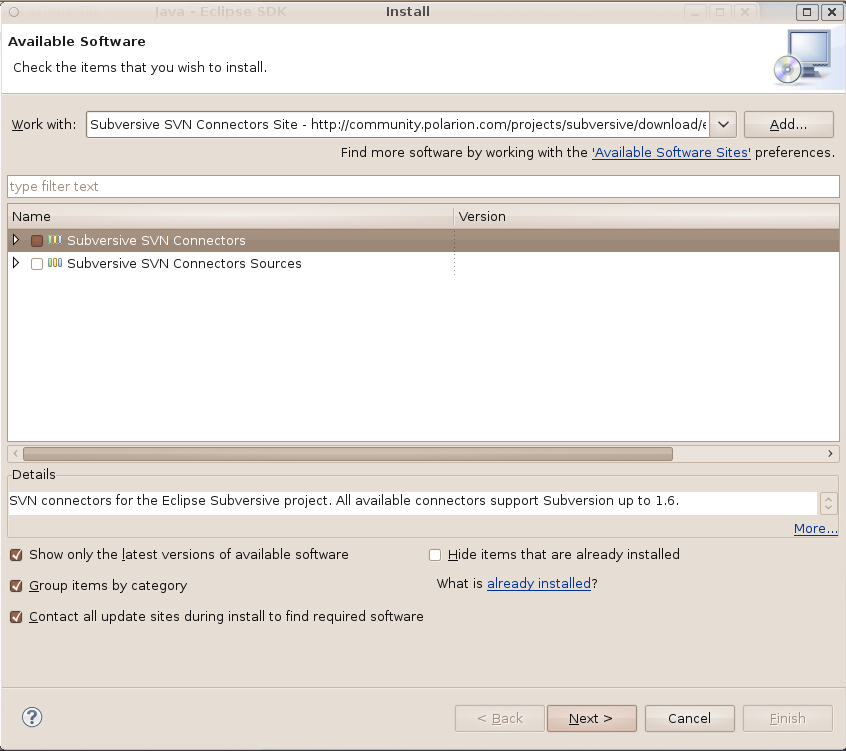
\includegraphics[width=1\textwidth]{./images/pic_compile/3_svn_3.png}
%  \end{minipage}
%  \begin{minipage}[c]{.45\textwidth}
%    \centering
%    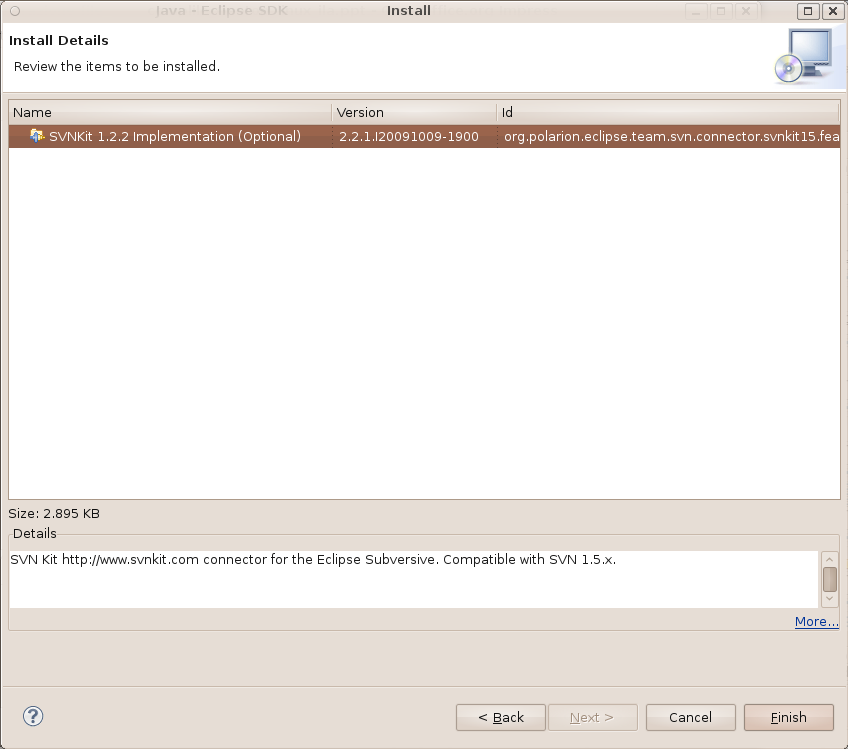
\includegraphics[width=1\textwidth]{./images/pic_compile/3_svn_4.png}
%  \end{minipage}
%  \end{center}
%    \textsl{\caption{SVN} \label{f:3_1}}
%\end{figure}

%

%\clearpage
%%%%%%%%%%%%%%%%%%%%%%%%%%%%%%%%%%%%%%%%%%%%%%%%%%%%%%%%%%%%%%%%
%\subsubsection{Download GEOtop code from SVN}
%%%%%%%%%%%%%%%%%%%%%%%%%%%%%%%%%%%%%%%%%%%%%%%%%%%%%%%%%%%%%%%%
%From \textsl{Window} $\rightarrow$ \textsl{Open prospective} $\rightarrow$ \textsl{Other} $\rightarrow$ \textsl{SVN Repository Exploring} $\rightarrow$ \textsl{OK}\\
%From \textsl{File} $\rightarrow$ \textsl{Import} $\rightarrow$ \textsl{SVN} $\rightarrow$ \textsl{Project from SVN}\\
%Add the Url: \textsl{"https://dev.fsc.bz.it/repos/geotop"} $\rightarrow$ \textsl{"Browse"}\\  
%From \textsl{geotop $\rightarrow$ trunk} $\rightarrow$ select \textsl{"0.9375KMackenzie \#\#"} where the \#\# is the current GEOtop version\\ 
%And then check \textsl{Save in the workspace location path} as shown in \textsl{Figure \ref{f:4}}

%\begin{figure}[!h]
%\begin{center}
%  \begin{minipage}[c]{.4\textwidth}
%    \centering
%    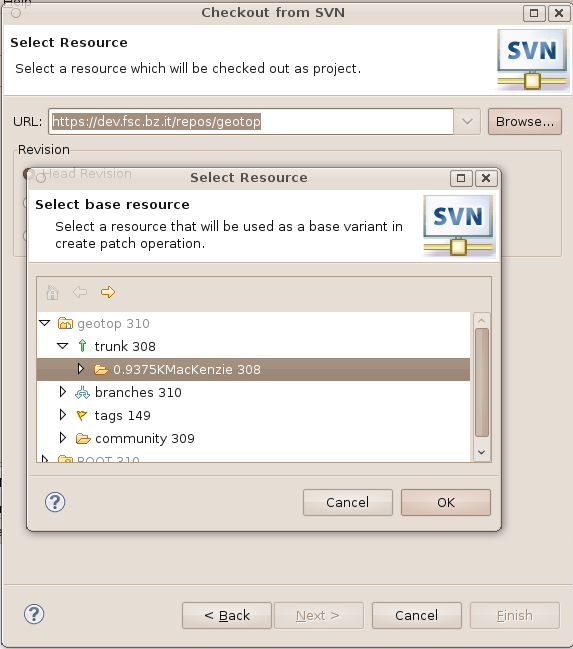
\includegraphics[width=1\textwidth]{./images/pic_compile/3_svn_6.png}
%  \end{minipage}
%  \begin{minipage}[c]{.4\textwidth}
%    \centering
%    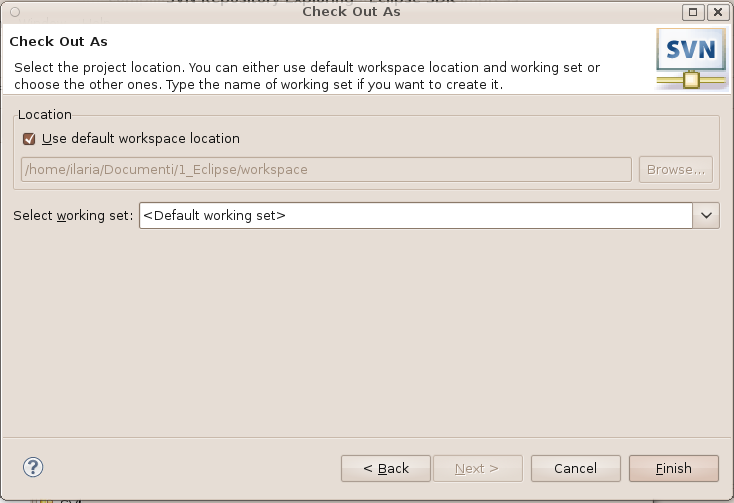
\includegraphics[width=1\textwidth]{./images/pic_compile/3_svn_7.png}
%  \end{minipage}
%\end{center}
%    \textsl{\caption{SVN} \label{f:4}}
%\end{figure}

%\newpage
%\paragraph{Set the C/C++ prospective:}
%%\noindent Set the GNU compiler and math library\\
%From \textsl{Window} $\rightarrow$ \textsl{Open prospective} $\rightarrow$ \textsl{Other} $\rightarrow$ \textsl{C/C++}\\
%The \textsl{'GEOtopKMacKenzie\_SVN'} project will be in the C/C++ prospective \textsl{Figure \ref{f:5}}\\

%\noindent \underline{Linux}\\
%\noindent Right click on \textsl{GEOtopKMackenzie\_SVN folder}
% $\rightarrow$ \textsl{Proprieties}  $\rightarrow$ \textsl{C/C++ Build}  $\rightarrow$ \textsl{Tool Chain Editor}\\
% $\rightarrow$ \textsl{Current Tool chain}: Linux GCC\\
% $\rightarrow$ \textsl{Current builder}: CDT Internal Builder\\

%\noindent Right click on GEOtopKMackenzie\_SVN folder\\
% $\rightarrow$ Proprieties  $\rightarrow$ C/C++ Build  $\rightarrow$ Settings
% $\rightarrow$ GCC C Linker $\rightarrow$ Miscellaneous
% $\rightarrow$ Linker flag: type \textsl{"-lm"} to activate math library \textsl{Figure \ref{f:6}}\\

%
%\begin{figure}[!h]
%\begin{center}
%  \begin{minipage}[c]{.8\textwidth}
%    \centering
%    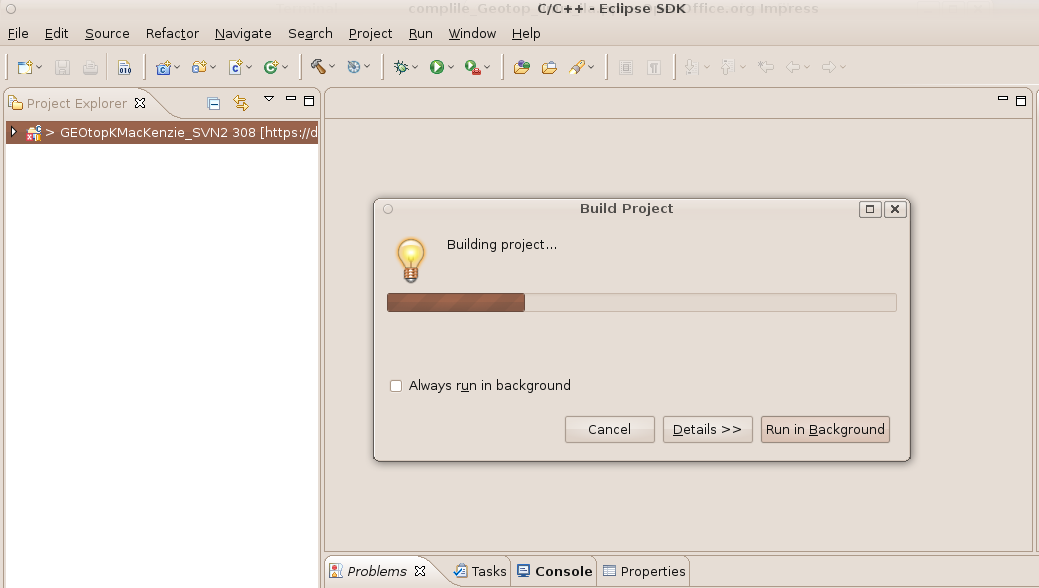
\includegraphics[width=1\textwidth]{./images/pic_compile/7_compile.png}
%  \end{minipage}
%\end{center}
%    \textsl{\caption{SVN} \label{f:5}}
%\end{figure}

%\begin{figure}[!h]
%\begin{center}
%  \begin{minipage}[c]{.4\textwidth}
%    \centering
%    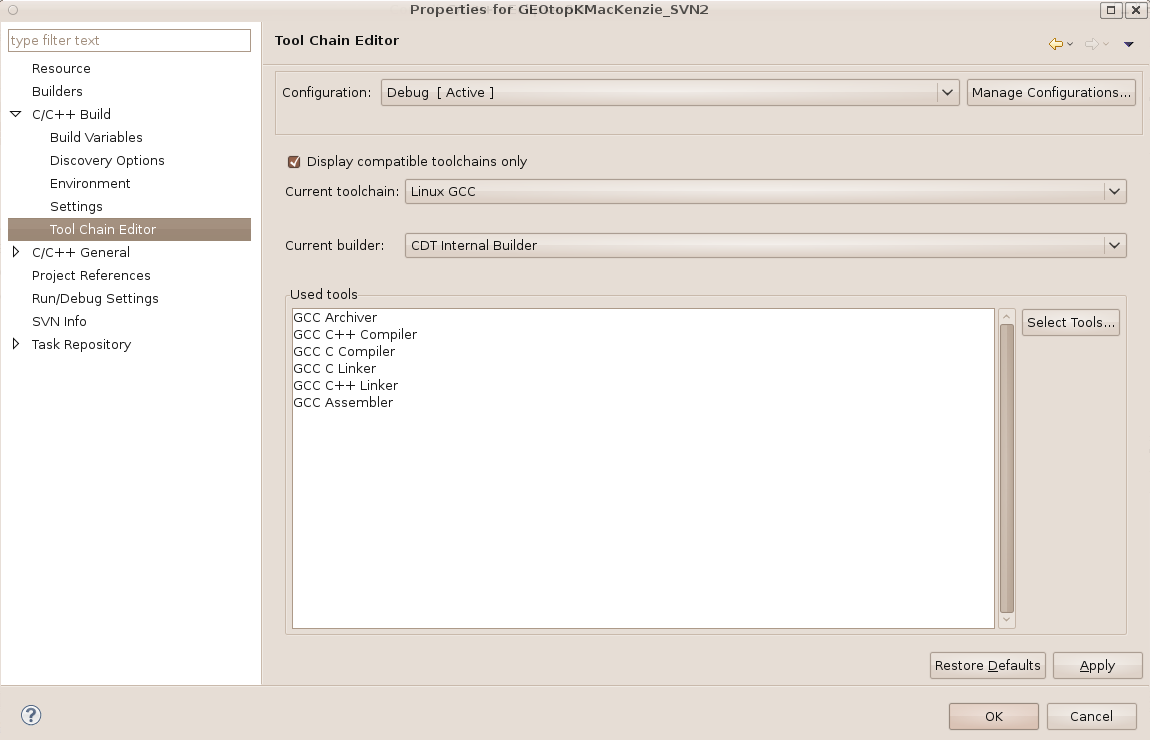
\includegraphics[width=1\textwidth]{./images/pic_compile/Tool_Chain.png}
%  \end{minipage}
%  \begin{minipage}[c]{.4\textwidth}
%    \centering
%    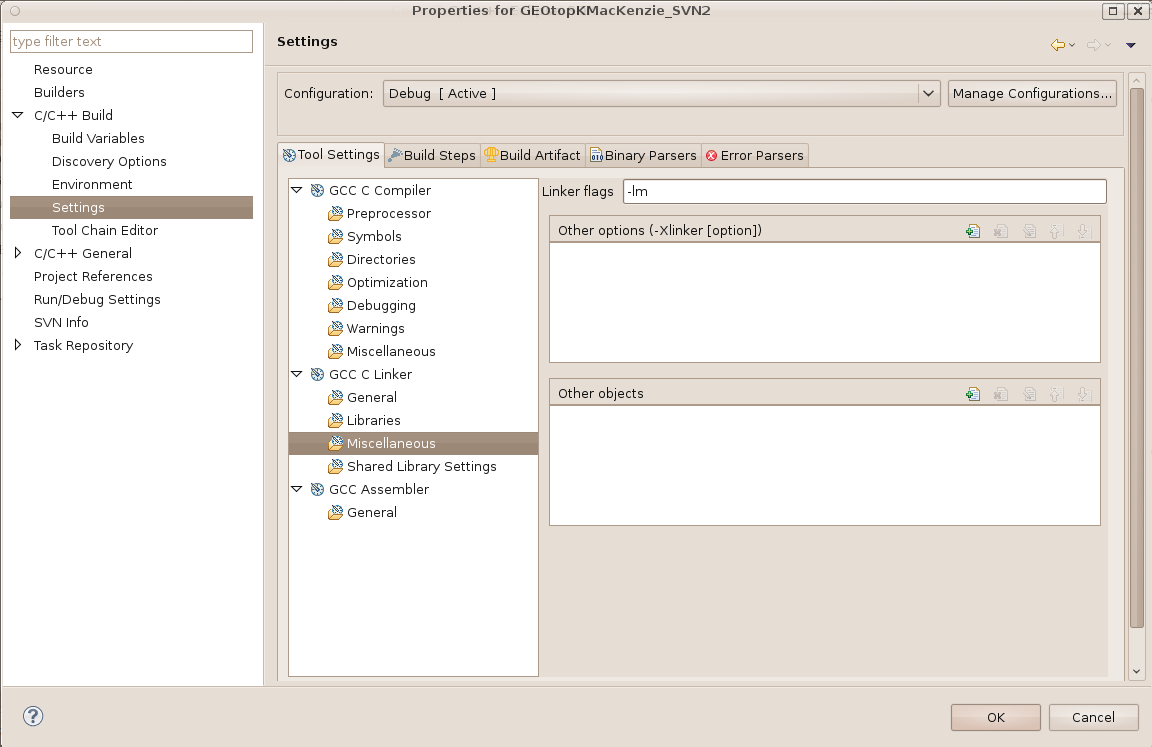
\includegraphics[width=1\textwidth]{./images/pic_compile/Linker_flag.png}
%  \end{minipage}
%\end{center}
%    \textsl{\caption{Tool Chain Editor and Linker Flag} \label{f:6}}
%\end{figure}

%\newpage
%\noindent \underline{MacOSx}\\
%\noindent Right click on \textsl{GEOtopKMackenzie\_SVN folder}
% $\rightarrow$ \textsl{Proprieties}  $\rightarrow$ \textsl{C/C++ Build}  $\rightarrow$ \textsl{Tool Chain Editor}\\
% $\rightarrow$ \textsl{Current Tool chain}: MacOSx GCC\\
% $\rightarrow$ \textsl{Current builder}: GNU Make Builder \textsl{Figure \ref{f:7}}

%\begin{figure}[!h]
%\begin{center}
%  \begin{minipage}[c]{.8\textwidth}
%    \centering
%    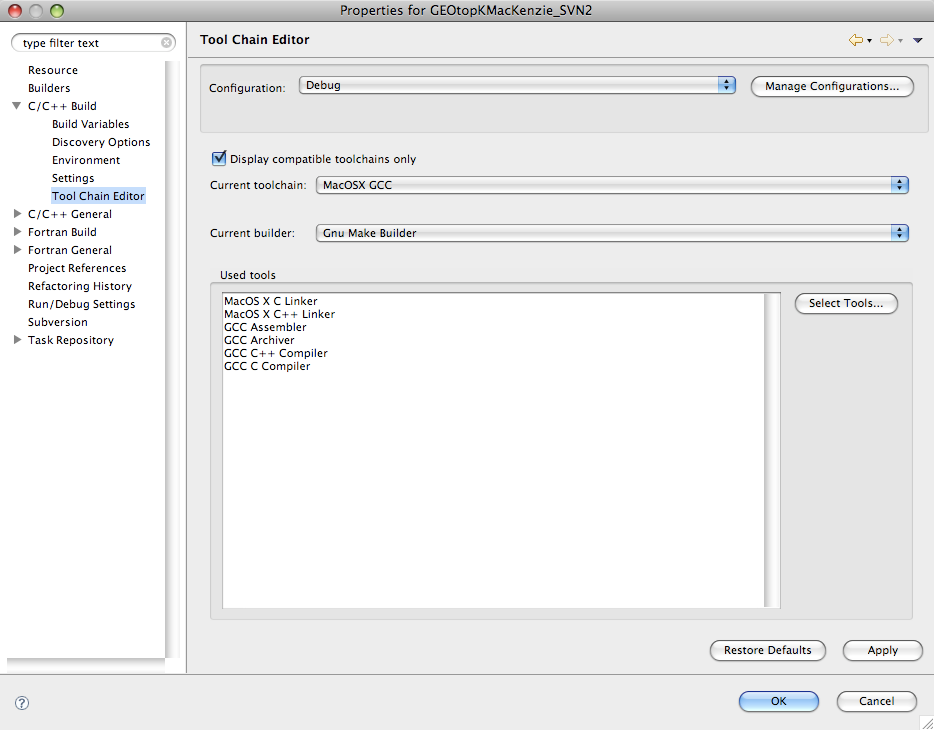
\includegraphics[width=1\textwidth]{./images/pic_compile/screen_Mac.png}
%  \end{minipage}
%\end{center}
%    \textsl{\caption{SVN} \label{f:7}}
%\end{figure}

%\noindent Now is possible to successfully build GEOtop\\
%Click on the hammer symbol: \textsl{Build 'Debug' for project 'GEOtopKMacKenzie\_SVN2'}\\
%GEOtop executable has been built $\rightarrow$ The executable file is under the folder 'Binaries'\\
%\noindent The simulation finished succesfully  \textsl{Figure \ref{f:8}}.

%\begin{figure}[!h]
%\begin{center}
%  \begin{minipage}[c]{.6\textwidth}
%    \centering
%    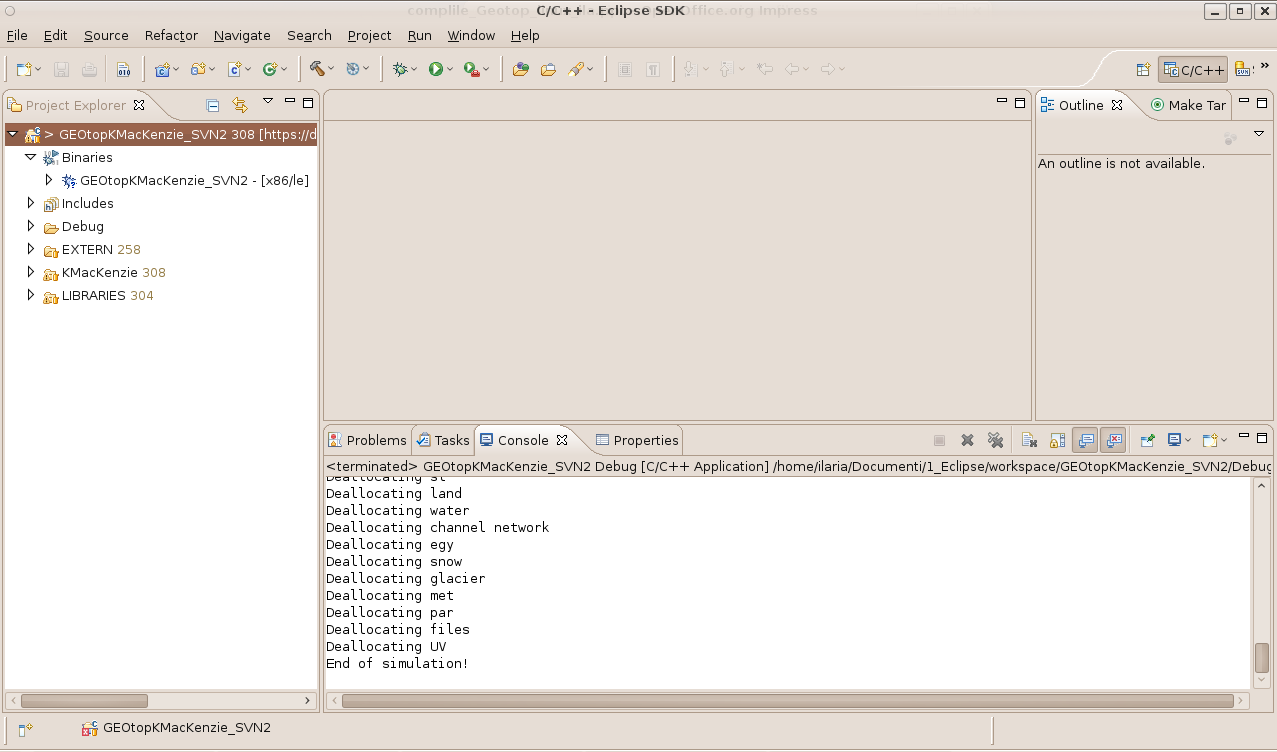
\includegraphics[width=1\textwidth]{./images/pic_compile/12_end.png}
%  \end{minipage}
%\end{center}
%    \textsl{\caption{SVN} \label{f:8}}
%\end{figure}

%

%\newpage
%%%%%%%%%%%%%%%%%%%%%%%%%%%%%%%%%%%%%%%%%%%%%%%%%%%%%%%%%%%%%%%

\chapter{Basic theory}

\section{The calculation grid}\label{Par:calc_grid}

%GEOtop is a distributed hydrological model capable of calculating the complete water and energy cycle in a domain, given the meteorological forcing in input. 
\subsection{Planar grid}
The calculation domain is based on a fixed regular Cartesian grid that coincides with the DEM (Digital elevation model), as reported in Fig. \ref{Fig_gen_dem}, on which it is possible to extract the hydrological basin closed at a given outlet  (Fig. \ref{Fig_dem_dxdy}). The X-axis coincides with the west-east direction and the Y-axis with the South-North direction, whereas the calculation grid size coincides with the pixel size (dX, dY) of the DEM. 


\begin{figure}[!h]
\begin{center}
\begin{minipage}[c]{1.0 \textwidth}
\centering
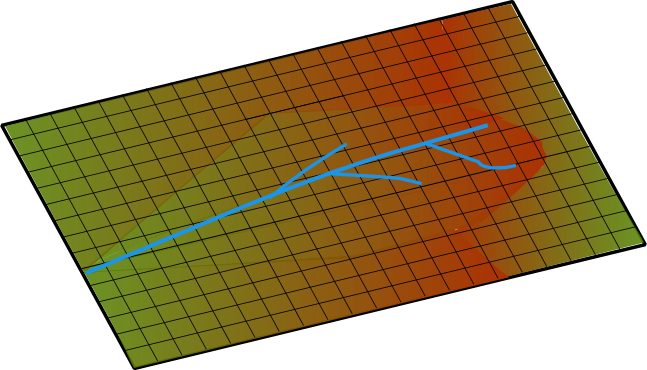
\includegraphics[width =0.72 \textwidth]{./images/pic_domain/dem_river}
\end{minipage}%
%\hspace{10mm}%
%\begin{minipage}[c]{0.46 \textwidth}
%\centering
%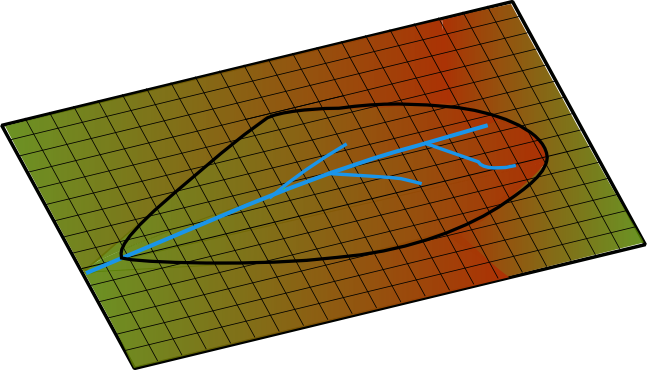
\includegraphics[width =1 \textwidth]{./images/pic_domain/dem_river_basin}
%\end{minipage}%
\end{center}
\caption{DEM of an the area of interest}
\label{Fig_gen_dem}
\end{figure}



\begin{figure}[tbp]
\begin{center}
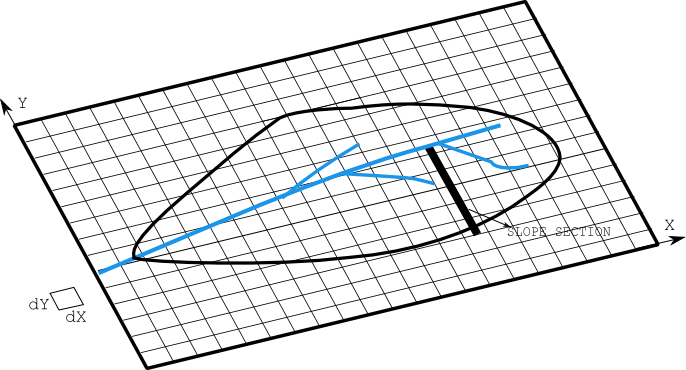
\includegraphics[width=0.7 \textwidth]{./images/pic_domain/dem_dxdy}
\caption{Calculation grid coinciding with the DEM. The hydrological basin (black line) and the river network (blue line) are present.}
\label{Fig_dem_dxdy}
\end{center}
\end{figure}

\subsection{Vertical grid}
The Z-axis is vertical and oriented towards the center of the Earth. It is possible to define the number of layers along the z-axis and the discretization, i.e. the vector of layer depths (Fig. \ref{Fig_discr3d} left). Note that the layer depth be irregular (different layers of various depths) but uniform in all the domain and the layer numbering starts from the top to the bottom (Fig. \ref{Fig_discr3d} right). The calculation grid points coincide with the center of the cell (on the X-Y axis) and the center of the layer (on the X-Z axis). Table \ref{table_vert_grid} reports and example of a vertical grid discretization characterized by 8 layers with irregular depths.

\begin{center}
\begin{longtable}{|p {1.5 cm}|p {2.2 cm}|}
\hline
\textbf{Layer ID} & \textbf{Depth (mm)}  \\ \hline
\endfirsthead
\hline
\multicolumn{2}{| c |}{continued from previous page} \\
\hline
\textbf{Layer ID} & \textbf{Depth (mm)} \\ \hline
\endhead
\hline
\multicolumn{2}{| c |}{{continued on next page}}\\ 
\hline
\endfoot
\endlastfoot
\hline
1 &10  \\ \hline
2 &15  \\ \hline
3 &20  \\ \hline
4 &20  \\ \hline
5 &60  \\ \hline
6 &50  \\ \hline
7 &80  \\ \hline
8 &100  \\ \hline
\caption{Vertical grid discretization and layer depth}
\label{table_vert_grid}
\end{longtable}
\end{center}



\begin{figure}[!h]
\begin{center}
\begin{minipage}[c]{0.46 \textwidth}
\centering
\includegraphics[width =0.9 \textwidth]{./images/pic_domain/discre_3d_nospess}
\end{minipage}%
\hspace{10mm}%
\begin{minipage}[c]{0.46 \textwidth}
\centering
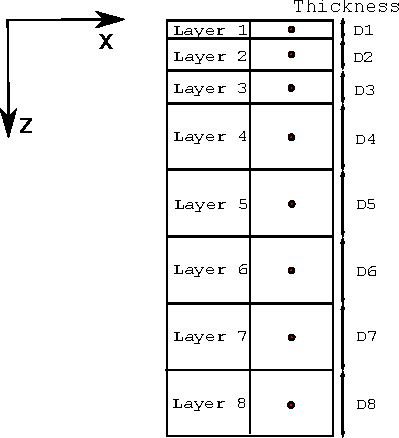
\includegraphics[width =0.9 \textwidth]{./images/pic_domain/soil_verticale.pdf}
\end{minipage}%
\end{center}
\caption{Left: three dimensional calculation grid. Right: discretization on the x-z plane. The red points, at the center of the cell, coincide with the calculation grid points}
\label{Fig_discr3d}
\end{figure}

\newpage
\begin{figure}[tbp]
\begin{center}
\begin{minipage}[c]{0.35 \textheight}
\centering
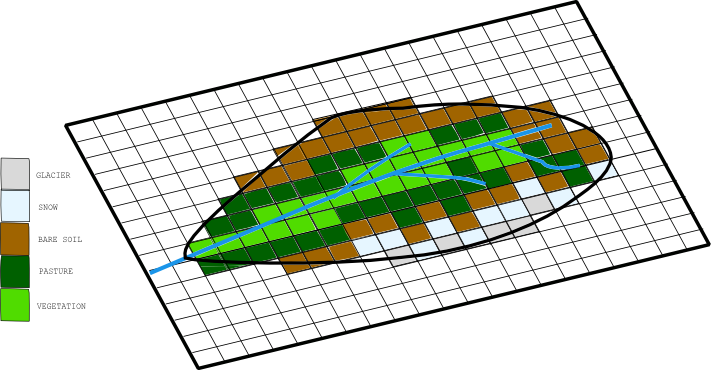
\includegraphics[width=1.4 \textwidth]{./images/pic_domain/land_cover_foglia}
\end{minipage}
\vspace{10 mm}
\begin{minipage}[c]{0.5 \textheight}
\centering
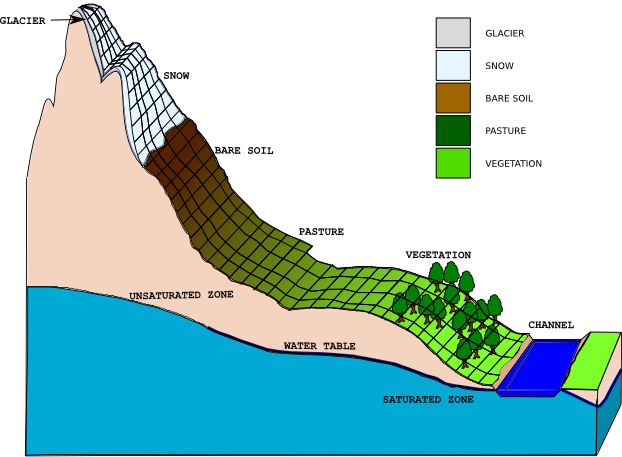
\includegraphics[width=0.9 \textwidth]{./images/pic_domain/general2D}
\end{minipage}
\caption{Top: Classification of a slope surface in a mountain basin on the basis of the land cover. Bottom: same classification for the entire basin.}
\label{Fig_general}
\end{center}
\end{figure}

\section{The domain characterization}

The domain characterization has the objective to determine:
\begin{itemize}
\item the land use i.e. vegetation, pasture, snow, glacier, forest etc. This map is usually called {\t land cover}
\item the stratigraphical characteristics of the soil, i.e. 1 m of thick debris (gravel), 2 m of sand, 2 m of loam etc. in order to ease the guess of the hydraulic and thermal parameters of the soil. This map is usually called {\it soil type}.
\end{itemize}


\subsection{Land cover}

Let us define a slope on the DEM, as reported in Fig. \ref{Fig_dem_dxdy}: ideally it can be figured out as in Fig. \ref{Fig_general}: at the bottom left is located the channel, then towards the higher elevations one may found the vegetated area, pasture, bare soil, snow covered area and glacierized area. 
%Inside the domain one may think about the water table, above which is the unsaturated zone and below which the saturated zone.
 Fig. \ref{Fig_general} on the top reports the slope surface discretization and classification, whereas on the bottom reports the land cover classification of the whole domain.
In this example may be identified five classes of land cover: vegetated area, located near the main stream in the low elevated range; pasture area, located in the medium range elevations; bare soil area, located on the steepest part of the domain and at medium-high elevations; snow covered area, located at high elevation and finally the glaciarized area on the highest parts.
% on the bottom.



\begin{figure}[tbp]
\begin{center}
\begin{minipage}[c]{0.35 \textheight}
\centering
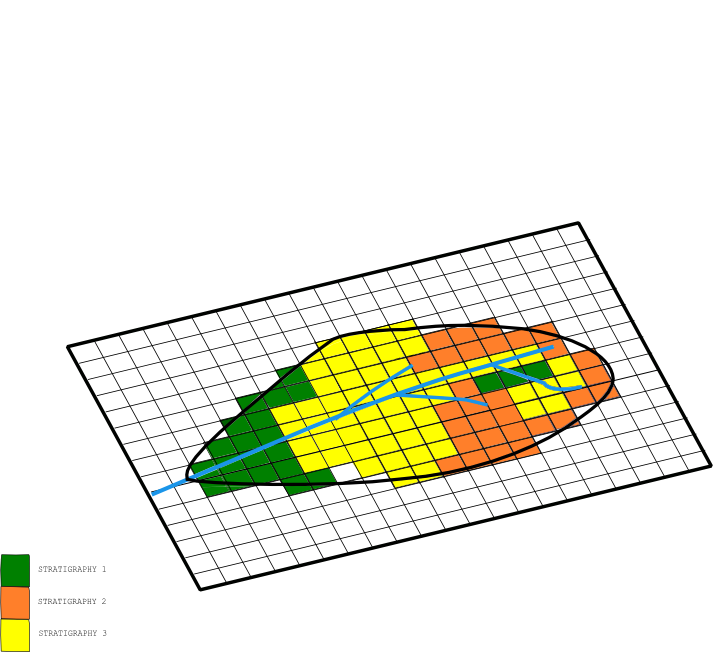
\includegraphics[width=1.3 \textwidth]{./images/pic_domain/soil_type_foglia}
\end{minipage}
\vspace{10 mm}
\begin{minipage}[c]{0.5 \textheight}
\centering
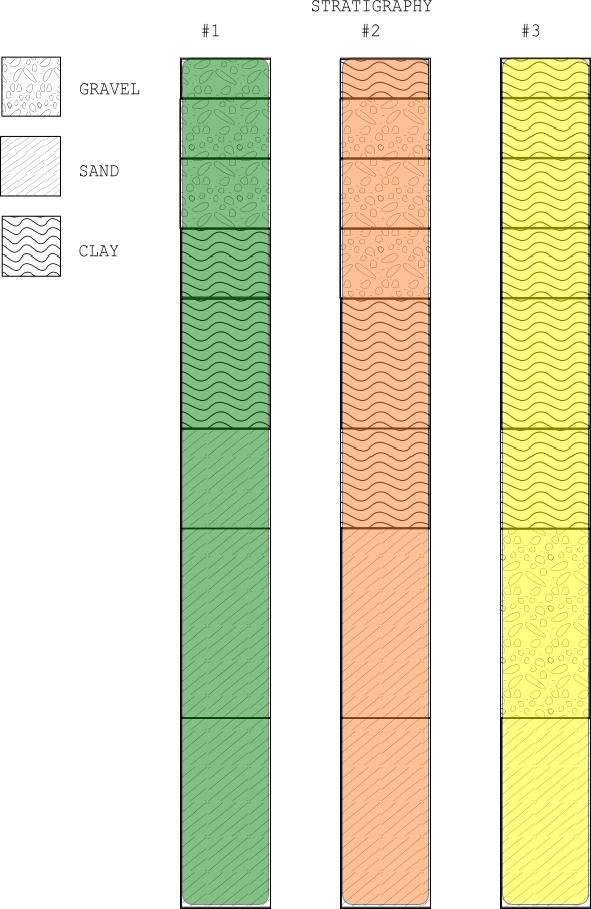
\includegraphics[width=0.5 \textwidth]{./images/pic_domain/1Dsoiltype.png}
\end{minipage}
\caption{Domain characterization oriented to define the soil stratigraphy (soil type map).}
\label{Fig_soiltype_foglia}
\end{center}
\end{figure}


\subsection{Soil type}

Let us imagine to take a section of the slope and to classify the type of soil in terms of texture (debris, gravel, sand, loam, clay) and bedrock depth. Each classification number would correspond to a particular soil stratigraphy, defining the soil particles and depth of bedrock. Starting from these characteristics, one could derive the hydraulic and thermal parameters, e.g. according to \citet{VanGenuchten1980, schaap2001rcp}. Fig. \ref{Fig_soiltype_foglia} reports the resulting map where each color corresponds to a given soil stratigraphy; the description of each type of soil stratigraphy is given in Table \ref{table_soil_type}.

\begin{center}
\begin{longtable}{|p {2.2 cm}|p {2.5 cm}|p {2.2 cm}|}
\hline
\textbf{Stratigraphy ID} & \textbf{Layer ID involved}   & \textbf{Soil texture}  \\ \hline
\endfirsthead
\hline
\multicolumn{3}{| c |}{continued from previous page} \\
\hline
\textbf{Stratigraphy ID} & \textbf{Layer ID involved}   & \textbf{Soil texture}  \\ \hline
\endhead
\hline
\multicolumn{3}{| c |}{{continued on next page}}\\ 
\hline
\endfoot
\endlastfoot
\hline
1 &1, 2, 3 & gravel \\ \hline
1 &4, 5 & clay \\ \hline
1 &6, 7, 8 & sand \\ \hline \hline
2 &1 & clay \\ \hline
2 &2, 3, 4 & gravel \\ \hline
2 &5, 6 & clay \\ \hline
2 &7, 8 & sand \\ \hline \hline
3 &1, 2, 3, 4, 5, 6 & clay \\ \hline
3 &7 & gravel \\ \hline
3 &8 & sand \\ \hline
\caption{Soil type (stratigraphy) present in the domain}
\label{table_soil_type}
\end{longtable}
\end{center}






\subsection{The final 3D calculation grid}

The final calculation domain is reported in Fig. \ref{grid3Dversante_points}. At the top is represented a planar view of the basin with a detail on the soil discretization and stratigraphy; on the bottom, the slope profile is schematized: the surface is classified according to the land cover map, whereas the soil depth according to the soil type map.
Please note that the discretization on the Z axis is vertical and not normal to the slope.

\begin{figure}[tbp]
\begin{center}
\begin{minipage}[c]{0.3 \textheight}
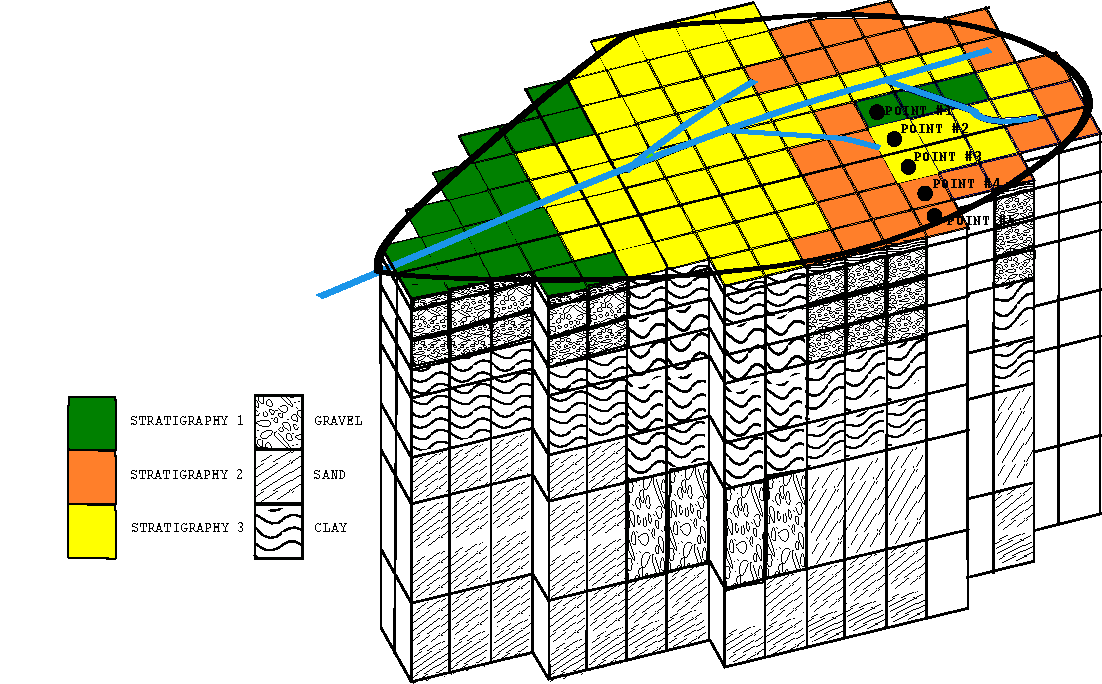
\includegraphics[width=1.8 \textwidth]{./images/pic_domain/soil_type_stratigraphy.pdf}
\end{minipage}
\vspace{10 mm}
\begin{minipage}[c]{0.5 \textheight}
\centering
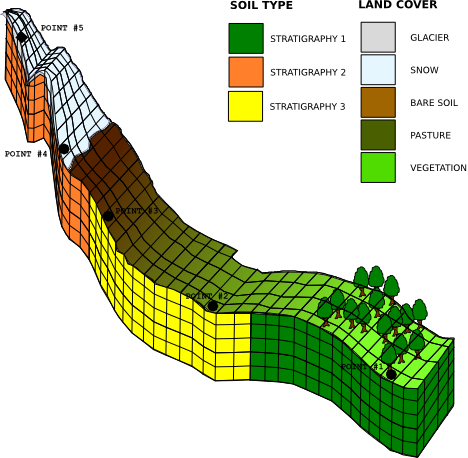
\includegraphics[width=0.9 \textwidth]{./images/pic_domain/grid3Dversante_points}
\end{minipage}
\caption{Domain characterization oriented to define the soil stratigraphy (soil type map).}
\label{grid3Dversante_points}
\end{center}
\end{figure}



%\begin{figure}[!h]
%\begin{center}
%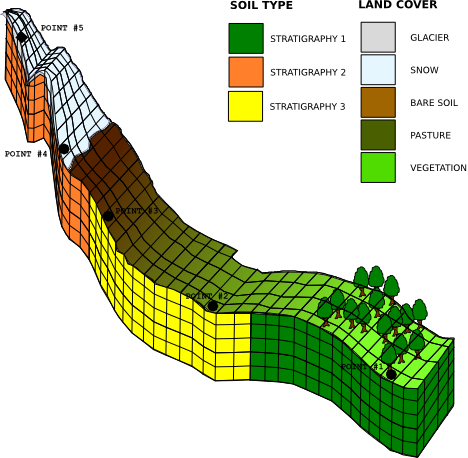
\includegraphics[width=0.8 \textwidth]{./images/pic_domain/grid3Dversante_points}
%\caption{Slope sectio: calculation domain and classification of land surface and soil type. }
%\label{grid3Dversante_points}
%\end{center}
%\end{figure}

\section{The focus on some points}\label{par:focusPoints}

It is possible to select some points in the basin that deserve a special attention, i.e. for the presence of a measurement device or for civil protection reasons. These points may be located wherever in the domain area and may be classified according to topographic characteristics (elevation, slope, aspect), surface type (land cover) and soil stratigraphy (soil type). Table \ref{table_points_charact} summarizes the characteristics of the simulation points reported on Fig. \ref{grid3Dversante_points}. The point 1 is located at low altitude on the bottom valley, in a vegetated area near the channel. The point 2 is located slightly upwards on the pasture, the point 3 is at medium-high altitude, where no vegetation is present (bare soil). The point 4, at 2500 m altitude, is still snow covered and finally the point 5, at 3100 m, is characterized by the presence of a glacier. As far as the soil type is concerned, the slope is characterized by the stratigraphy 1 at low altitude near the channel, where the point 1 is located. Then, at medium-range altitude, it is characterized by the stratigraphy 3 (see points 2 and 3) and finally, at high elevations, by the stratigraphy 2 (points 5 and 6).\\
These points may be highlighted to run multiple 1D simulations (see Par. \ref{par:1D3D}) or to print specific point results.


\begin{center}
\begin{longtable}{|p {1.5 cm}|p {1.5 cm}|p {1.5 cm}|p {1.8 cm}|p {1.8 cm}|p {1.8 cm}|}
\hline
\textbf{Point ID} & \textbf{Elevation (m a.s.l.)} & \textbf{Slope ($^\circ$)} & \textbf{Aspect ($^\circ$ N)} & \textbf{Land cover}& \textbf{Soil type} \\ \hline
\endfirsthead
\hline
\multicolumn{5}{| c |}{continued from previous page} \\
\hline
\textbf{Point ID} & \textbf{Elevation (m a.s.l.)} & \textbf{Slope ($^\circ$)} & \textbf{Aspect ($^\circ$ N)} \textbf{Land cover} & \textbf{Soil type} \\ \hline
\endhead
\hline
\multicolumn{5}{| c |}{{continued on next page}}\\ 
\hline
\endfoot
\endlastfoot
\hline
1 & 1200 & 15 & 30 & vegetation &1  \\ \hline
2 & 1600 & 10 & 30 & pasture &3 \\ \hline
3 & 2200 & 20 & 15 & bare soil  &3\\ \hline
4 & 2500 & 25 & 0 & snow  &2\\ \hline
5 & 3100 & 25 & 0 & glacier &2 \\ \hline
\caption{Topographic, land cover and soil type characteristics of the simulation points}
\label{table_points_charact}
\end{longtable}
\end{center}



\section{Meteorological forcing}

The meteorological data represent the dynamic forcing that constrain the domain to evolve, under the constraints given by topography, the conservation laws and the boundary conditions. GEOtop may receive in input the meteorological data coming from several stations (the number of meteo stations is an input parameter).


\subsection{Meteo station}
In order to describe the characteristics of the meteo stations, it is requested to provide the following information:
\begin{itemize}
\item the number of meteo station;
\item the coordinates (X, Y, Lat, Long) of each meteo station;
\item the elevation;
\item the sky view factor;
\item the standard time difference (of the time records with respect to Greenwich Meridiam Time);
\item the height of the wind speed and air temperature sensors.
\end{itemize}

\noindent Fig. \ref{Fig_meteoST1} shows the planar view of the domain area where three meteo stations (ST) are present: ST1 is located on a high peak, ST2 is on the bottom valley and ST3 is on a medium altitude peak at the lefthand side of the river. The prospect view of the meteo stations is reported in Fig. \ref{Fig_meteoST2}. It is important to note the following: (i) the meteo stations may also be outside of the land cover map, however must be located inside the DEM area; (ii) the sky view factor of the meteo station depends on topography: whereas ST1 has no obstruction because of its high elevation, ST2 is characterized by a big obstruction given by the mountain ranges.
Finally, the zoom in Fig. \ref{Fig_meteoST2} reports a particular of the meteo station: the wind sensor height and the air temperature height must be specified in the model.

\begin{figure}[t,b]
\begin{center}
\begin{minipage}[c]{1.0 \textwidth}
\centering
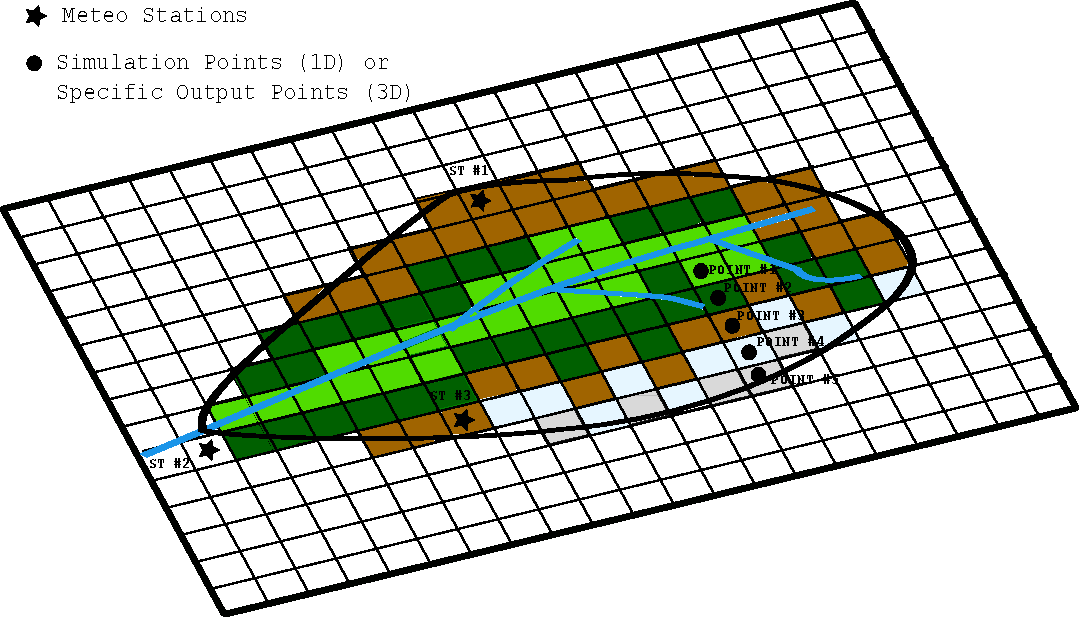
\includegraphics[width =1.0 \textwidth]{./images/pic_domain/foglia_LC_meteo.pdf}
\end{minipage}%
\end{center}
\caption{Planar view of meteo stations (ST) location in the domain area.}
\label{Fig_meteoST1}
\end{figure}


\begin{figure}[t,b]
\centering
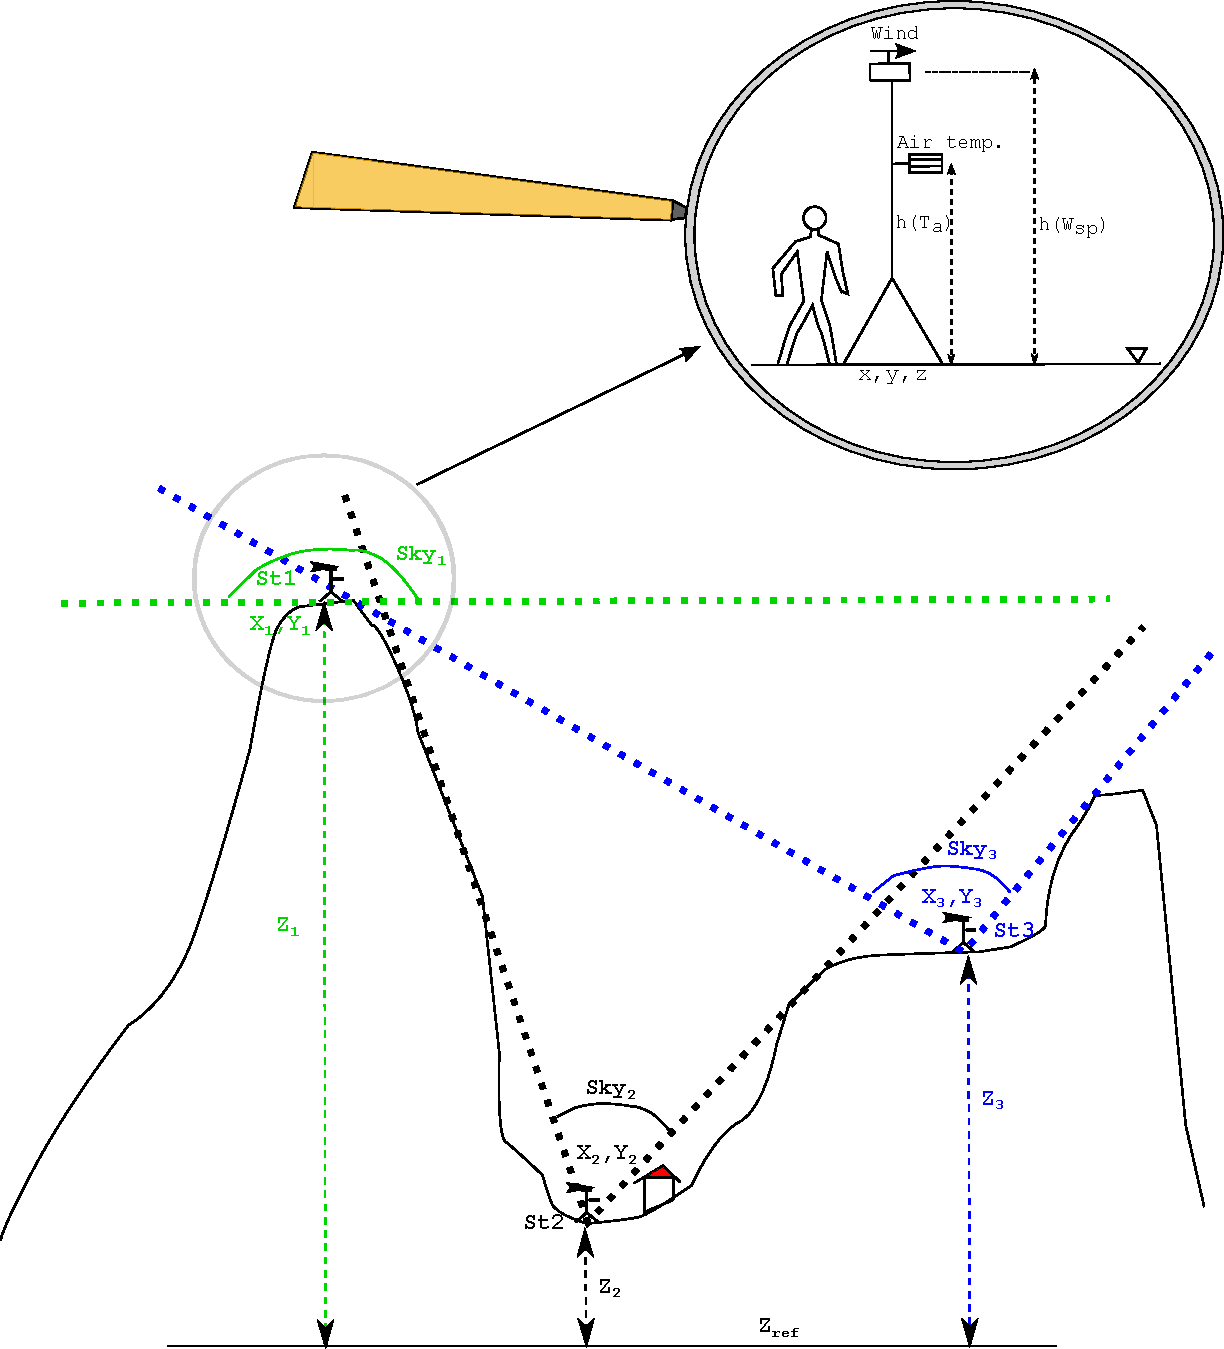
\includegraphics[width =0.85 \textwidth]{./images/pic_domain/MeteoSt.pdf}
\caption{Prospect view of meteo station (ST) location in the domain area. $X, Y, Z$ represent the east coordinate, north coordinate and elevation respectively. In the lence is reported a zoom of one meteo station: $h(T_a)$  and $h(W_{sp})$ represent the height of the air temperature and wind sensor respectively}
\label{Fig_meteoST2}
\end{figure}


\subsection{Meteo data}

Each meteo station, according to the sensor installed, may measure different type of variables. The admitted input variables considered as meteorological forcing are:

\begin{enumerate}
\item precipitation intensity (mm h$^{-1}$)
\item wind velocity (m s$^{-1}$)
\item wind direction ($^\circ$N)
\item windX and windY (m s$^{-1}$) (must belong to the same meteo station) 
\item relative humidity (\%)
\item air temperature ($^\circ$C)
\item dew temperature ($^\circ$C)
\item air pressure (bar)
\item short wave solar global radiation (W m$^{-2}$)
\item short wave solar direct radiation (W m$^{-2}$)
\item short wave solar diffuse radiation (W m$^{-2}$)
\item short wave solar net radiation (W m$^{-2}$)
\item long wave incoming radiation (W m$^{-2}$)
\end{enumerate}

\noindent The meteo variables have to be provided in the Meteo file, specified by the keyword {\it MeteoFile}. 
 It is compulsory to add to the file the column of the date, given by the DD/MM/YYYY hh:mm format or by the Julian day.
 Figg. \ref{meteo_cm1_old}, \ref{meteo_cm2} \ref{meteo_cm3} report an example of the time series that may be given in input.
The {\bf nodata} value is coded through the number {\bf -9999}.

\subsection{Cloudiness}

cloud transmissivity ( - )\\
cloud factor ( - ) 

\subsection{Lapse rates}

The meteorological variables are usually characterized by a gradient on elevation, known as ``lapse rate''. It represents the variation of the variable with elevation. GEOtop admits in input the a dynamic lapse rate that (variable in time) that, according to the elevation of the calculation grid node, modifies the value of the variable. The meteorological variable that admits a lapse rate are:
\begin{itemize}
\item lapse rate for precipitation (mm h$^{-1}$ hm$^{-1}$)\\
\item lapse rate for air temperature ($^\circ$C hm$^{-1}$)\\
\item lapse rate for dew temperature ($^\circ$C hm$^{-1}$)
\end{itemize}


\begin{figure}[t,b]
\centering
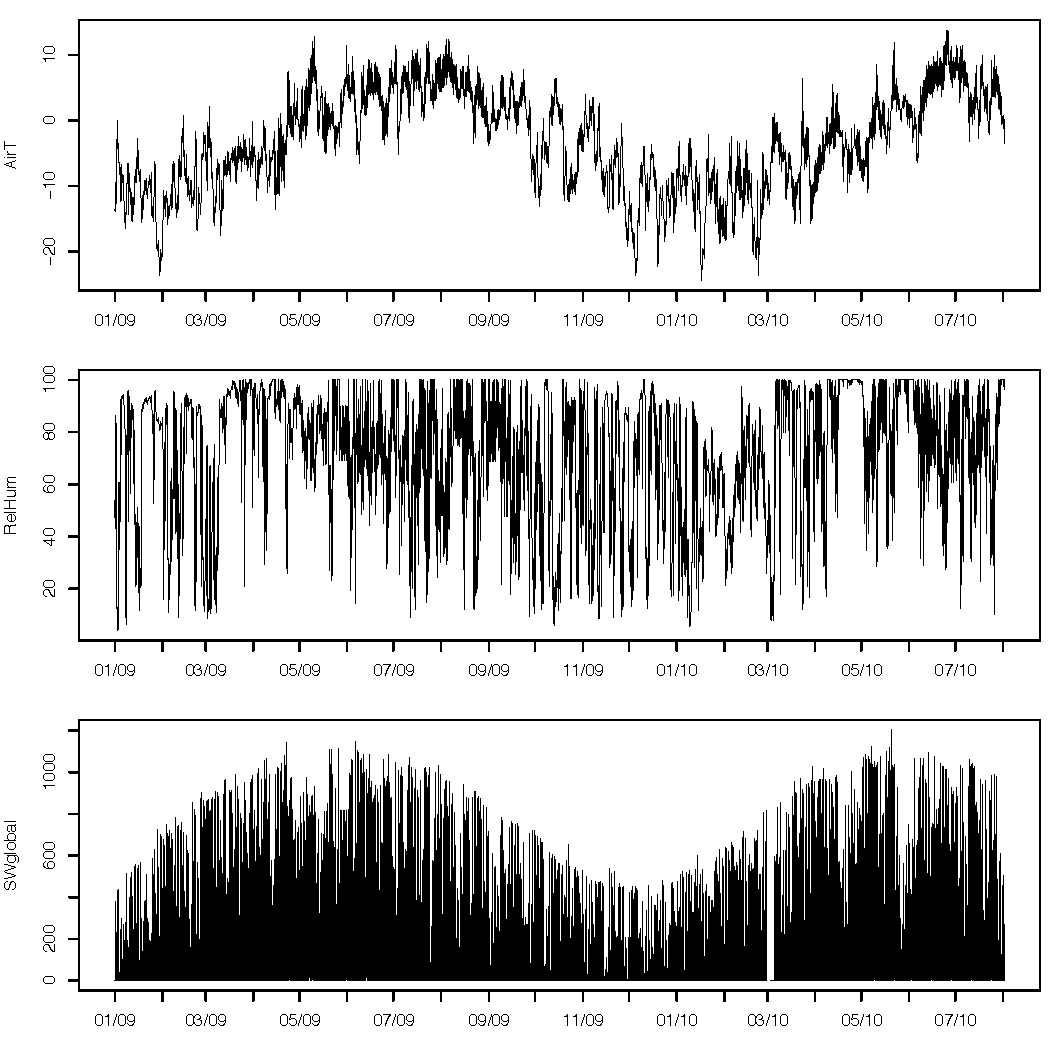
\includegraphics[width =0.9 \textwidth]{./images/pic_domain/meteo_cm1_old.pdf}
\caption{Meteo data measured in a meteo station. Top: air temperature (m s$^{-1}$); middle: relative humidity (\%); bottom: short wave global radiation (W m$^{-2}$)}
\label{meteo_cm1_old}
\end{figure}

\begin{figure}[t,b]
\centering
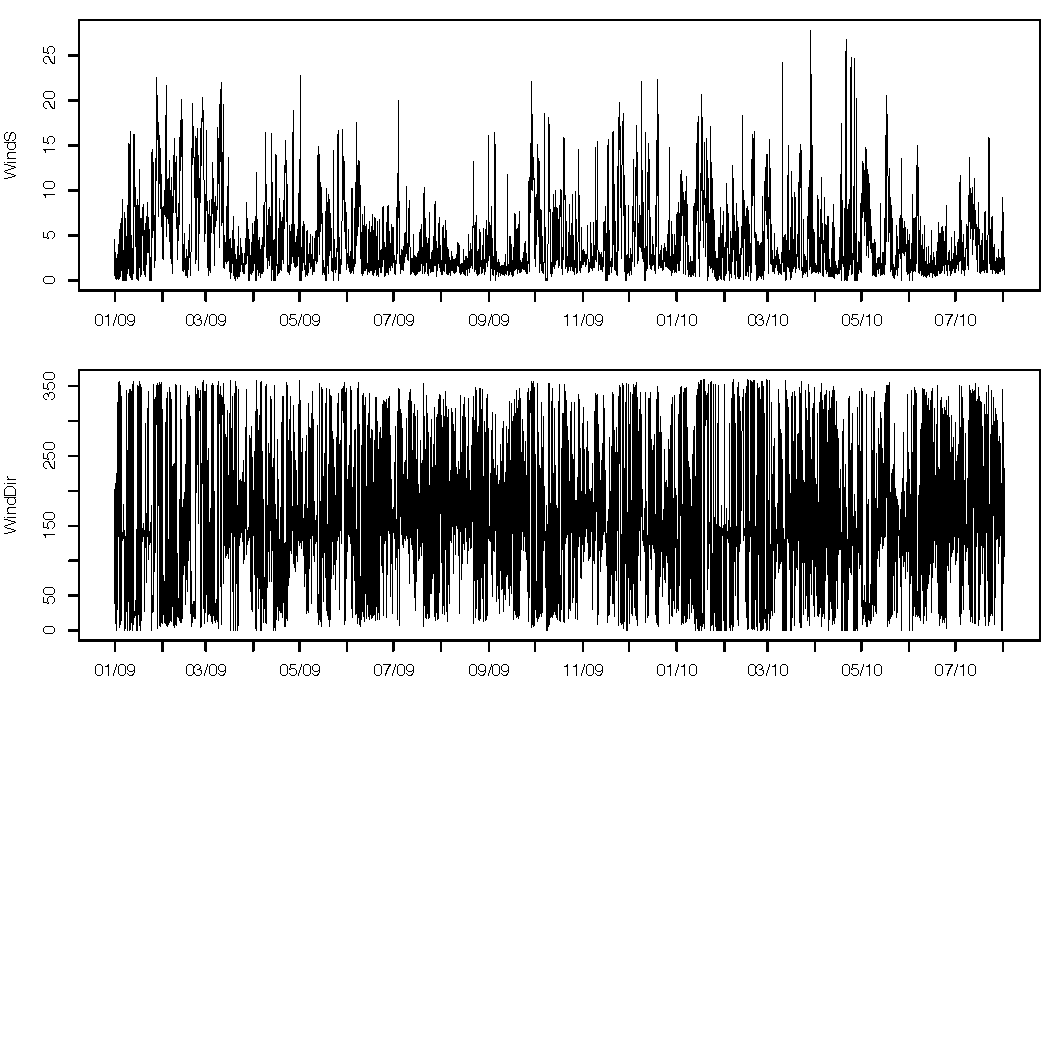
\includegraphics[width =0.9 \textwidth]{./images/pic_domain/meteo_cm2.pdf}
\caption{Meteo data measured in a meteo station. Top: wind speed (m s$^{-1}$); bottom: wind direction ($^\circ$ N)}
\label{meteo_cm2}
\end{figure}

\begin{figure}[t,b]
\centering
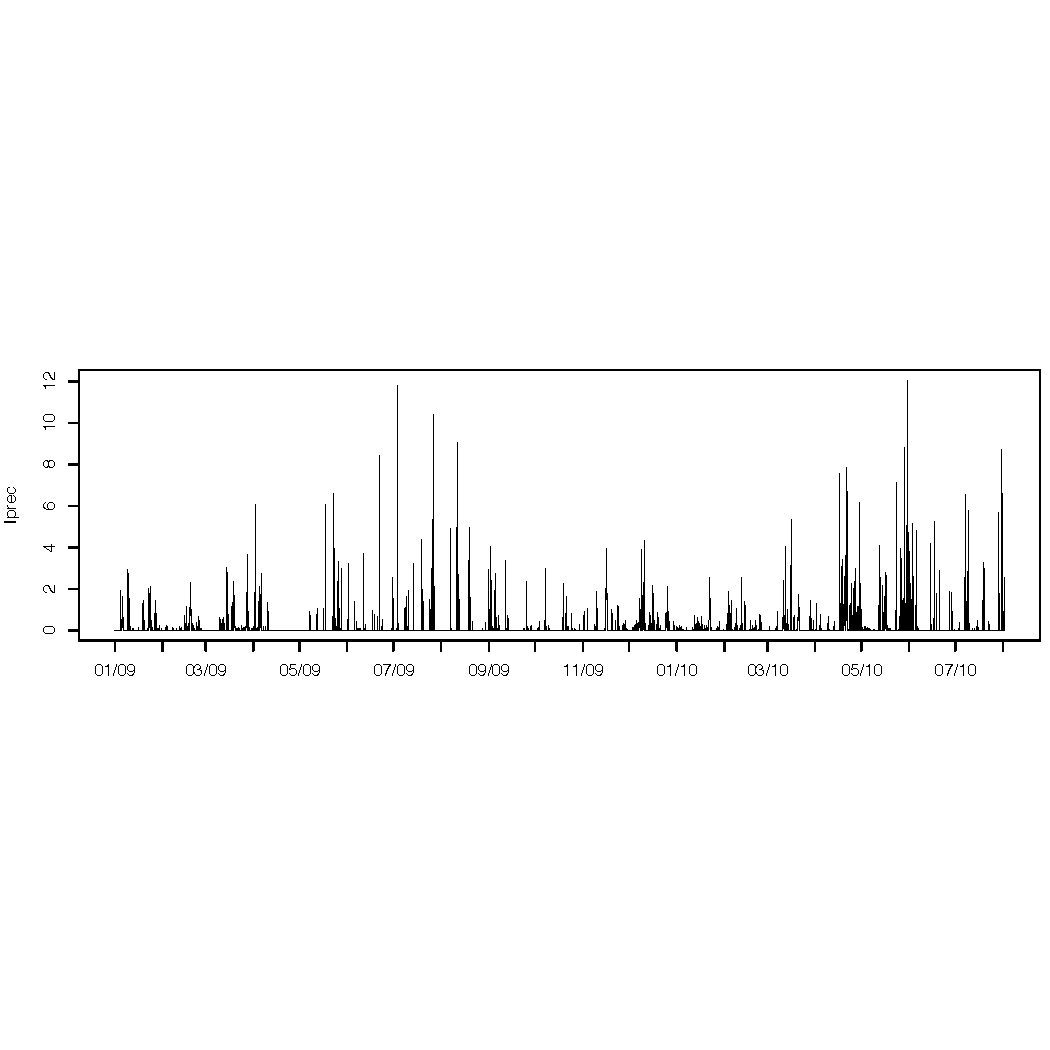
\includegraphics[width =0.9 \textwidth]{./images/pic_domain/meteo_cm3.pdf}
\caption{Meteo data measured in a meteo station: precipitation intensity (mm h$^{-1}$)}
\label{meteo_cm3}
\end{figure}

\chapter{Simulation flow chart}

This section is intended to provide a description of the simulation flow chart. In particular, a special focus will be given to the user's point of view (i.e. necessary input to provide and choices to make) when launching a simulation, and to the model point of view (i.e. calculation flow chart).

\section{User point of view}
The user that needs to fulfill a set of tasks in order to prepare the input necessary to launch a GEOtop simulation, as reported in Fig. \ref{Fig_sim_flowchart}.

\paragraph{Set general parameters}
 The user must define the type of simulation (1D or 3D) and other general input.

\paragraph{Meteo station characterization}
The user must define the position and characteristics of the meteo stations.

\paragraph{Meteo data}
The user must define the meteorological forcing measured in each meteo station.

\paragraph{Topographic characterization}
The user must define the topographical characteristics of the domain area (i.e. elevation, aspect, slope, sky view factor, curvature).

\paragraph{Land cover characterization}
The user must define the surface type characteristics of the domain (often called ``land use'' or ``land cover'').

\paragraph{Soil type characterization}
The user must define the soil type characteristics of the domain area (i.e. soil texture, soil water retention curve etc.).

\paragraph{Initial conditions}
The user must define the initial temperature and water content in each cell of the domain.

\paragraph{Boundary conditions}
The user must define the behavior (fluxes) at the border domain.

\paragraph{Physical parameters}
The user must parametrize the various physical processes involved. In particular, the current version of GEOtop allow to specify the parameters typical of the following processes: glacier, snow, vegetation, soil/rock thermal, soil/rock hydraulic and discharge).

\paragraph{Output parameters}
The user must determine the desired information to be printed and the correspondent frequency.



\begin{figure}[!h]
\centering
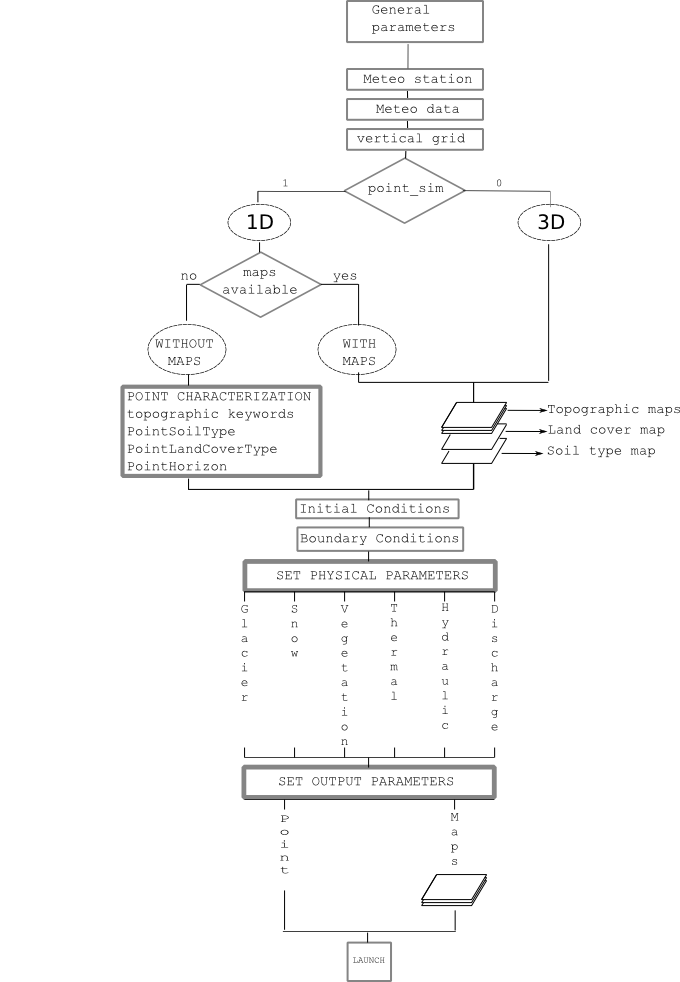
\includegraphics[height=0.8\textheight]{./images/pic_flowchart/SCHEMAi.png}
\caption{GEOtop flow chart: user point of view for preparing a simulation}
\label{Fig_sim_flowchart}
\end{figure}


\begin{table}[!h]
\begin{center}
\begin{minipage}[c]{0.42\textwidth}
\begin{tabular}{c|c}
HeaderHorizonAngle & HeaderHorizonHeight\\
``azi'' & ``hang''\\
\hline
45 \textdegree	&	0.00\\
135 \textdegree	&	10.00\\
225 \textdegree	& 	30.00\\
315 \textdegree	&	5.00\\
\hline
\end{tabular}
\end{minipage}
\hspace{0.5cm}
\begin{minipage}[c]{0.42\textwidth}
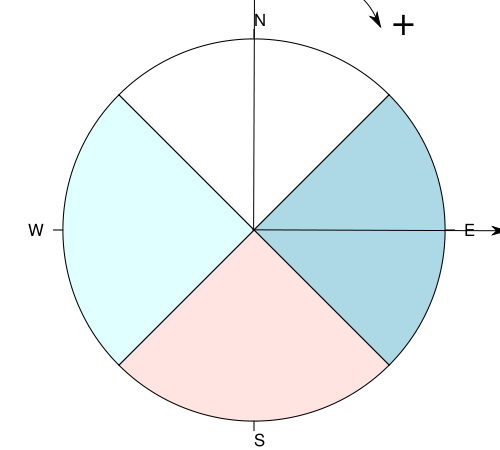
\includegraphics[width=1\textwidth]{./images/pic_1D/pie.png} 
\end{minipage}
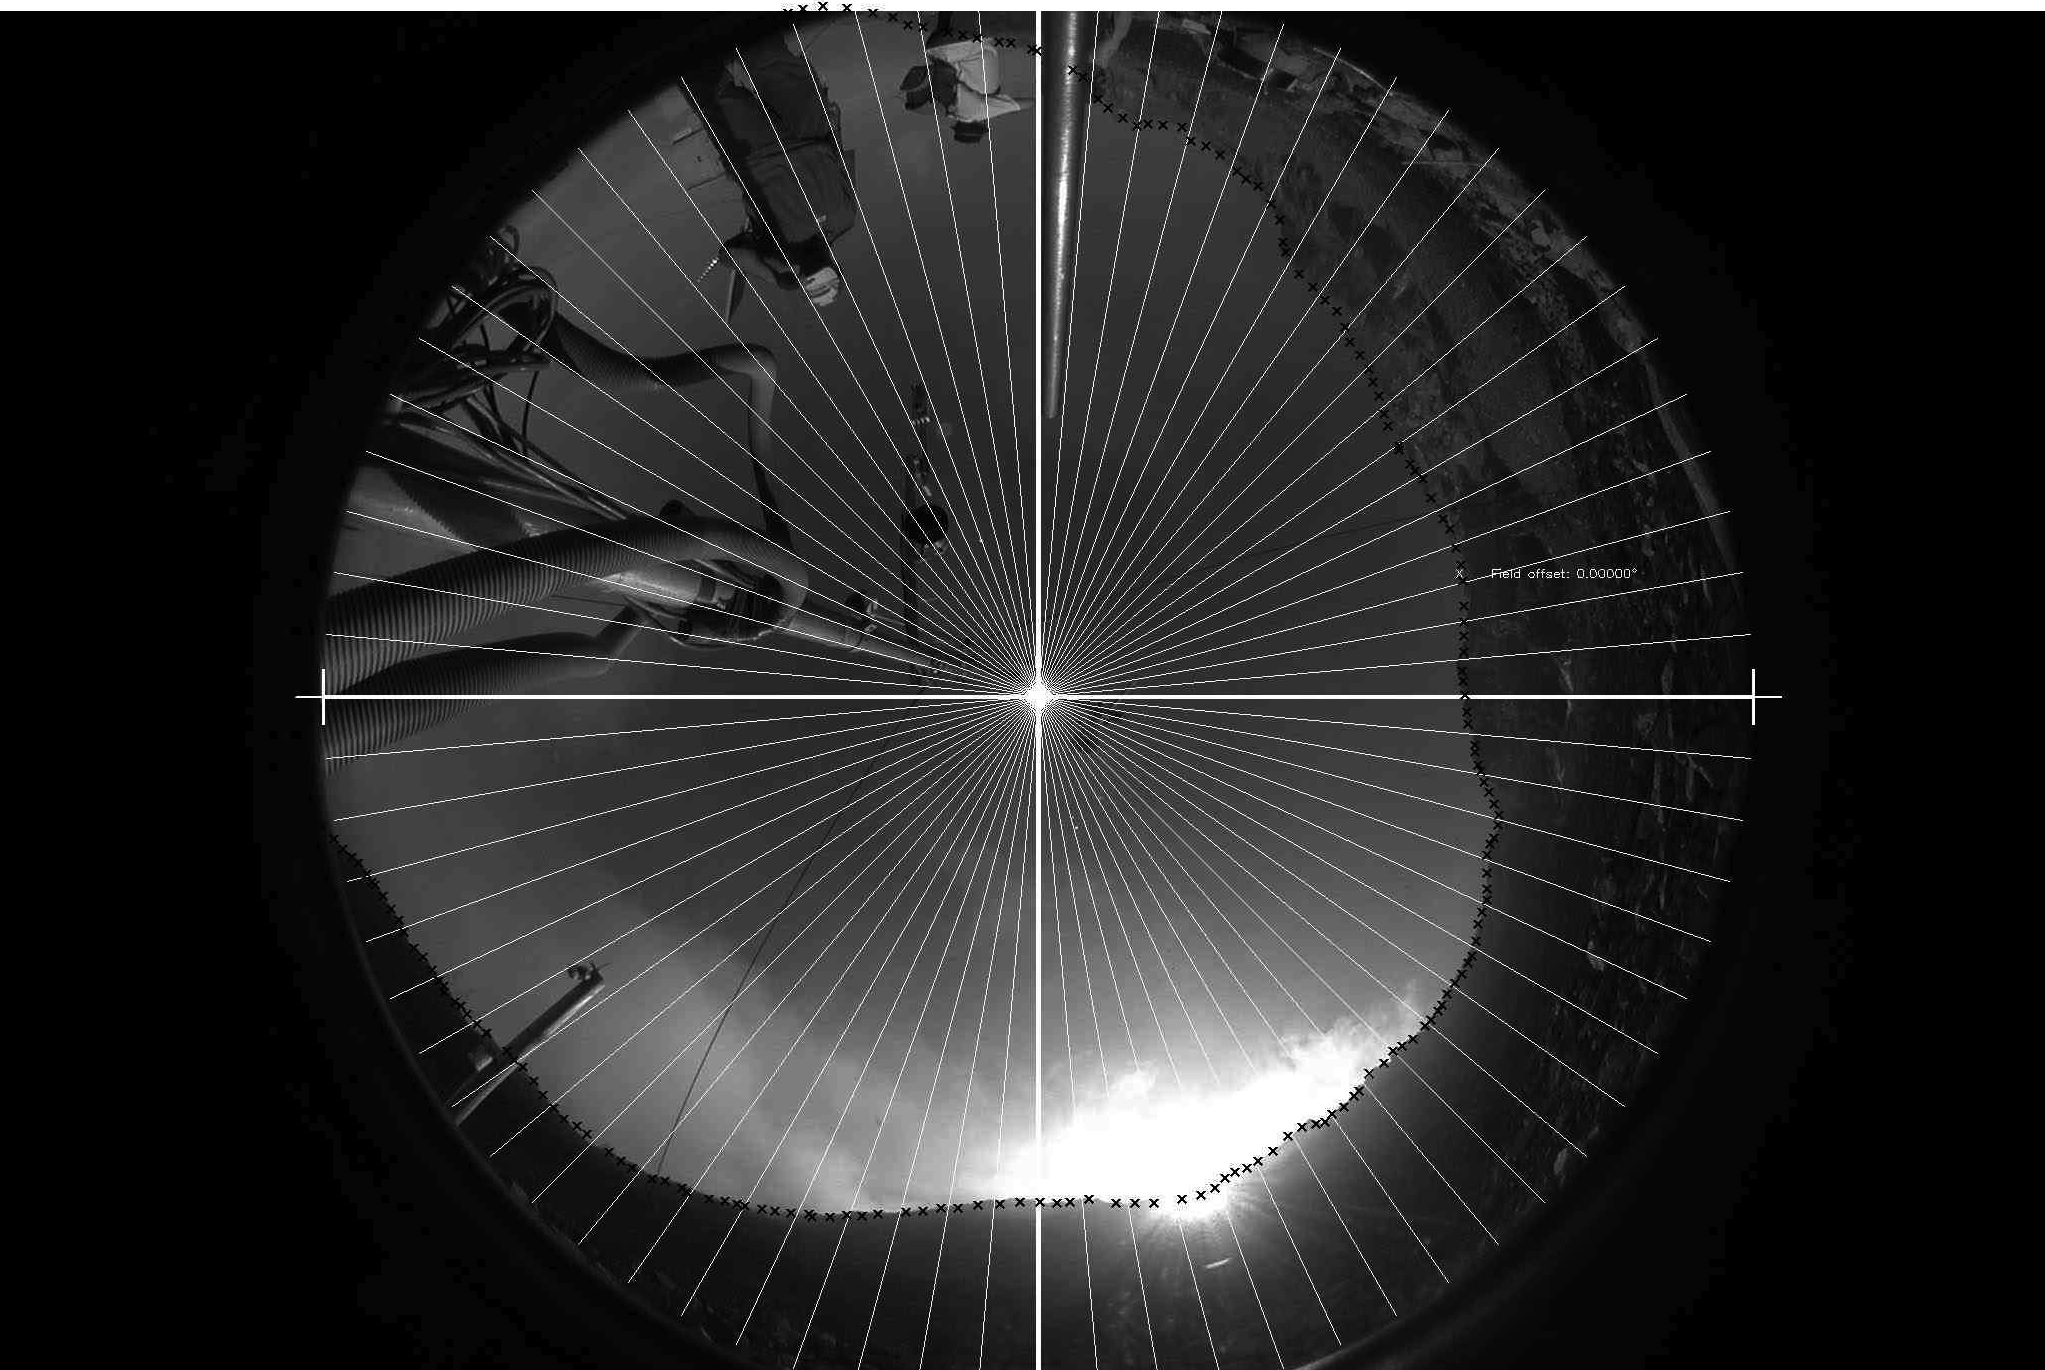
\includegraphics[width=0.8\textwidth]{./images/pic_1D/fish_eye_view.jpg}
\textsl{\caption{Top: example of the default horizon file and of the corresponding azimuth classes. An example is given in Par. \ref{Par_keyprop}. Bottom: example of a fish-eye view from a point (courtesy of Stephan Gruber)}
\label{azh}}
\end{center}
\end{table}

\section{1D simulations}\label{par:1D3D}

Originally GEOtop was born as a hydrological model with the objective to produce maps of hydrological variables in a catchment. Later, thanks to the boost received by the permafrost community, it was adapted also to analyze single points located in extreme topographies. In these points, as outlined in Par. \ref{par:focusPoints}, for various reasons it may be interesting to produce 1D simulations. In fact 1D simulations are often useful as they allow to obtain results very rapidly and, in some cases, sufficiently reliable. 

%=============================================================%
\subsection{Point horizon}\label{descr_horizon}
%=============================================================%

In order to account for the topography visible by the simulation point, it is recommendable to provide the horizon file of the point.
Every point $P(x,y,z)$ on the landscape, unless in the middle of a flat terrain, is surrounded by obstacles like mountains, buildings, trees. These objects, during the day, according to the elevation and position (azimuth) of the sun at a particular time in the year (julian day and day time), may produce a cast shadow on the point $P$ that prevents the point from receiving direct solar radiation. \\
Thanks to proper cameras (e.g. fish-eye camera, see bottom of Fig. \ref{azh}) or to GIS routines, it is possible to produce a file that outlines the angle height of the obstacles along a given azimuth direction.
The {\it HorizonPointFile} \index{HorizonPointFile} allows to specify the horizon seen by a point $P$ along a desired discretization of the azimuth. The file structure is thus a matrix whose first column represents the azimuth angle and the second column the elevation angle of the object height. The Table \ref{azh}) reports the horizon file where the azimuth has been discretized in 4 parts. Note that the North direction must always be in the center of the slides in which the circle is divided. It is possible to increase the azimuth classes in order to provide a more detailed description of the obstacles height.\\
The horizon data may be specified in the following cases:
\begin{enumerate}
 \item 1D simulations: since the topography is not provided, the user may provide the horizon file for every simulated point. 
Unless given, the model creates one assuming an overall flat terrain;
 \item for meteorological stations: in this case it is needed to set the time when the sun is obscured by the obstacle; from that time onward the cloudiness calculation is no more carried by the ratio between actual and potential radiation, since the actual radiation would no longer provide a reliable value.
\end{enumerate}

\subsection{1D simulations: with or without maps}\label{}

Let us suppose to select five points in the basin (see Fig. \ref{grid3Dversante_points}) where we want to run five 1D simulations. First of all it is necessary to provide the coordinates (X, Y) of the points, together with the average latitude and longitude of the area. In addition to that, it is necessary to characterize the points by specifying the topography (elevation, aspect, slope, sky view factor, curvatures and the horizon), the soil type and land cover.  This last information may be provided in two ways:
\begin{itemize}
\item {\bf with maps}: the topographical, land cover and soil type maps are provided and the model, according to the coordinates of the points, automatically sets the topographical characteristics;
\item {\bf without maps}: the user has to specify all the characteristics of the points (e.g. see Table \ref{table_in_topochar}).
\end{itemize}

\subsection{1D simulations in steep topography}\label{}

The domain scheme of a 1D simulation at steep mountain topography is depicted in Fig. \ref{Fig_1Dsteep}: the scheme is represented on the left: the axis of elevation $Z_f$ is on the vertical direction and sets the elevation of the point on the surface, whereas the layers are located normal to the slope. If present, also the slope, aspect and horizon of the point $P_1$ may be specified. 
As the 1D representation is just an abstract sequence of layers of various depths located along on an imaginary line, one may think that the final scheme resembles what outlined on the right, where the elevation axis and the line $Z$ axis form an angle complementary to the slope angle. Note that the $Z$ axis does not coincide with the gravitational $Z_f$ axis.
\begin{figure}[t]
\centering
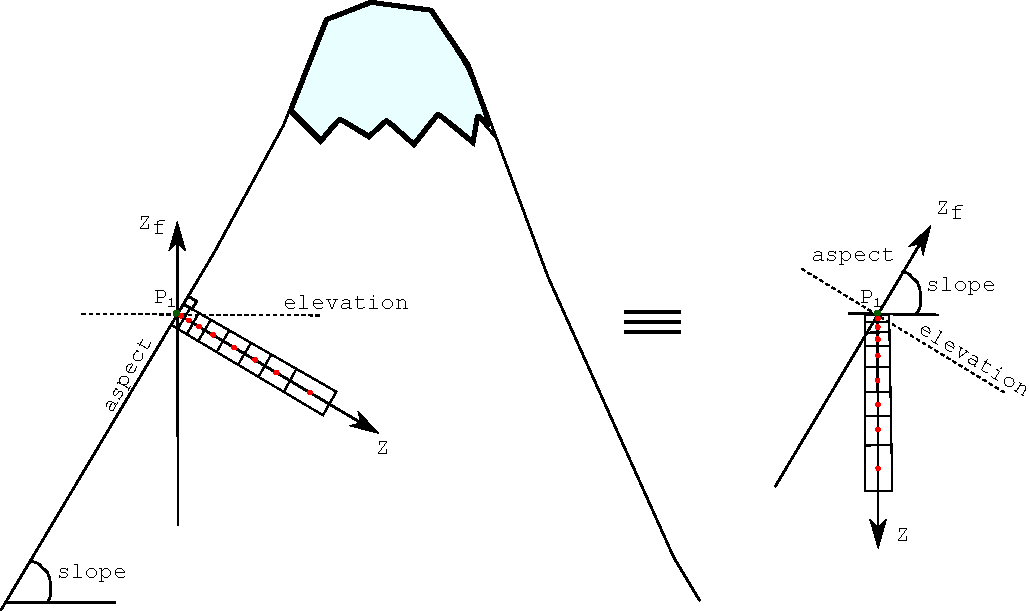
\includegraphics[width=0.85\textwidth]{./images/pic_flowchart/1Dsimul.pdf}
\caption{Scheme of a 1D simulation on steep topography typical of high mountain altitude}
\label{Fig_1Dsteep}
\end{figure}

\section{Model point of view}
 On the other hand, the model transforms the input given by the user into results, by solving the energy and mass balance in the calculation domain. As reported in Fig. \ref{Fig_sim_flowchart2}, at the beginning of the simulation, GEOtop does the following activities: 
\paragraph{1. Read input data} In this phase, the model reads: (i) the keywords and parameters specified in {\it geotop.inpts} and other properly defined files; (ii) the topographic maps (elevation, aspect, slope, sky view factor, curvature), the land cover map (that coincides with the calculation mask), the map of soil type and, if available, the maps of initial conditions; (iii) reads the parameters (physical and output). If a parameter or a map is not specified with the proper keyword, it assumes the default value.

\paragraph{2. Create and initialize mesh} As reported in Par. \ref{Par:calc_grid}, it creates the calculation mesh according to the grid size of the land cover map and the vertical nodes spacing defined for the vertical grid. Then it initializes the temperature and water pressure head of each node with the initial conditions and sets the physical parameters according to what specified by the keywords. 

\paragraph{3. Read meteo data} During this phase it incorporates the meteorological data for each meteo station: these data represent the forcing that will drive the simulation, producing the dynamic boundary conditions for the surface nodes. Finally, GEOtop sets the initial simulation time to initialize the simulation counter: this will allow to compare the current simulation time with the expected simulation end time. \\

\noindent At this point begins the time loop for the calculation and the printing routines. In particular, at each calculation time step, GEOtop fulfills the following tasks:
\paragraph {1. Distribute meteorological forcing}
This allows to spatially distribute the meteorological forcing, measured in discrete meteo station, in all the calculation cells. This methodology is based on \citet{liston2006meteorological}.

\paragraph{2. Energy balance}
In this phase the energy balance equation is solved. This encompasses the calculation of the surface energy fluxes, the vegetation module, the snow/glacier module and the routine that the calculates the soil temperatures and ice content.

\paragraph{3. Water balance}
In this phase the mass balance equation is solved. This encompasses the calculation of the infiltration routine to determine the pore water pressure and water content through a 3D Richards solver. Eventually, the runoff and channel routing routines, based on a shallow-water solver, will allow to determine the discharge at the basin outlet.

\paragraph{4. Write output}
This phase is intended to print the point information and the maps according to the desired output frequency.

\paragraph{5. Update and check time}
This phase updates the time with the calculation time step and compares the new time with the simulation end time, to verify whether to stop the simulation or loop again. If the current simulation time exceeds the end of the simulation, then the program stops and deallocates all the structures.


\begin{figure}[t]
\centering
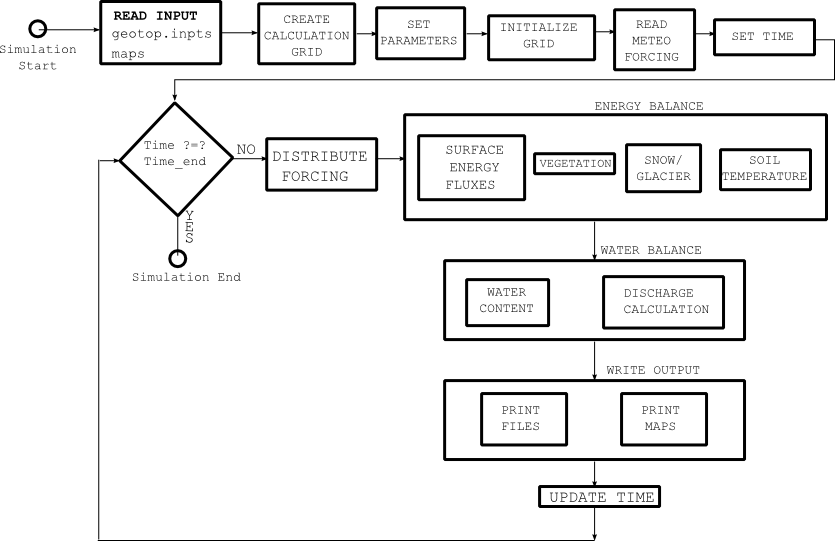
\includegraphics[width=0.9\textwidth]{./images/pic_flowchart/SCHEMAii.png}
\caption{GEOtop flow chart: model point of view for accomplishing a simulation}
\label{Fig_sim_flowchart2}
\end{figure}


\newpage
\section{How to Run GEOtop}
%%%%%%%%%%%%%%%%%%%%%%%%%%%%%%%%%%%%%%%%%%%%%%%%%%%%%%%%%%%%%%%
\subsection{From Terminal  on Linux/Mac platform}

\noindent  If you successfully installed GEOtop v.2.1 as explained in chapter 2 you should have executable at the command line 


\noindent Type:

\footnotesize{
\begin{verbatim}
$ geotop  
\end{verbatim}
}



\noindent this should give as output something similar to this:


\footnotesize{
\begin{verbatim}
>geotop
Geotop 2.1 usage
Options:
  -v [ --version ]      print version string
  -h [ --help ]         this help
  -w [ --workdir ] arg  the working directory of the simulation

\end{verbatim}
}
 
\noindent to get information about version and compilation time

\footnotesize{
\begin{verbatim}

>geotop -v
This GEOtop version  was compiled at:  Mar 22 2017  09:08:00
The Git revision hash of the source code is: TRIEST_release-54-g3e20a0fa
This version does NOT USE METEO-IO library for interpolation: METEOIO-OFF

\end{verbatim}
}


\noindent  To run a simulation  leave one space and type now the path to the folder where the simulation files are:

\footnotesize{
\begin{verbatim}
$geotop   /directory/where/data/are
\end{verbatim}
}

\noindent Remember to put a``/'' (slash) at the end and the type {\it Return}. The simulation should start and on the screen you should see somethinh like that..




\footnotesize{
\begin{verbatim}
geotop GEOTOP/geotop_examples/1D/InfiltrationTrench/
THIS IS THE INITIAL STATEMENT:

GEOtop 2.1  31 december 2016

Copyright (c), 2016 - GEOtop Foundation


GEOtop 2.1 is a free software and is distributed under GNU General Public License v. 3.0 <http://www.gnu.org/licenses/>
WITHOUT ANY WARRANTY; without even the implied warranty of MERCHANTABILITY or FITNESS FOR A PARTICULAR PURPOSE.

########################## INFO ABOUT COMPILATION #################################
This GEOtop version  was compiled at:  Mar 22 2017  09:08:00
The compiler gives a __cplusplus value of
The Git revision hash of the source code is: TRIEST_release-54-g3e20a0fa
This version does NOT USE METEO-IO library for interpolation: METEOIO-OFF
This run starts at: Sat Apr 15 12:08:44 2017
##### Please report the above lines if you ask for help ############################
[NOTICE]: Configuration file parsing completed. 3412 characters parsed.
[NOTICE]: Full match!
[NOTICE]: Max snow layer number: 24, of which 4 at the bottom, 10 in the middle, and 10 at the top.
[NOTICE]: Infinite Snow layer numbers are numbers:
	5 6 7 8 9 10 11 12 13 14
[NOTICE]: Max glac layer number: 0, of which 0 at the bottom, 0 in the middle, and 0 at the top.
[NOTICE]: Infinite Glac layer numbers are numbers:
.....

[NOTICE]: 20/3/2012 10:00 99.86\% - Time elapsed (h:m:s)  0:00:15 Time remaining (h:m)  0:00
[NOTICE]: 20/3/2012 11:00 99.93\% - Time elapsed (h:m:s)  0:00:15 Time remaining (h:m)  0:00
[NOTICE]: 20/3/2012 12:00 100.00\% - Time elapsed (h:m:s)  0:00:15 Time remaining (h:m)  0:00
[NOTICE]: Duration of simulation: 18.194097

[NOTICE]: Close files
[NOTICE]: Deallocating global variables
[NOTICE]: Deallocating soil
[NOTICE]: Deallocating top
[NOTICE]: Deallocating land
[NOTICE]: Deallocating water
[NOTICE]: Deallocating channel network
[NOTICE]: Deallocating UV
[NOTICE]: Deallocating egy
[NOTICE]: Deallocating snow
[NOTICE]: Deallocating glacier
[NOTICE]: Deallocating met
[NOTICE]: Deallocating times
[NOTICE]: Deallocating par
[NOTICE]: Deallocating novalues
[NOTICE]: End of simulation!



\end{verbatim}
}





%\subsection{From Eclipse}
%\begin{itemize}
% \item \textsl{Run} $\rightarrow$ \textsl{Run Configurations}
% \item Click on the icon: \textsl{New launch configuration}
% \item \textsl{C/C++ Applications} $\rightarrow$ click on \textsl{'New configuration'}
% \item \textsl{Name} $\rightarrow$ Choose a name you like for the project, as for example: GEOtop
% \item \textsl{Arguments} $\rightarrow$ \textsl{Program Arguments} $\rightarrow$ \textsl{Type} ./
% \item \textsl{Working directory} $\rightarrow$ Uncheck the \textsl{'Use default'} string 
% \item \textsl{Working directory} $\rightarrow$ Click on 'File System' $\rightarrow$ Select the path of the folder
%containing the input files for the simulation 
% \item Click on \textsl{'Apply'} button
% \item Click on \textsl{'Run'} button
%\end{itemize}


%\begin{figure}[!h]
%\begin{center}
%  \begin{minipage}[c]{.45\textwidth}
%    \centering
%    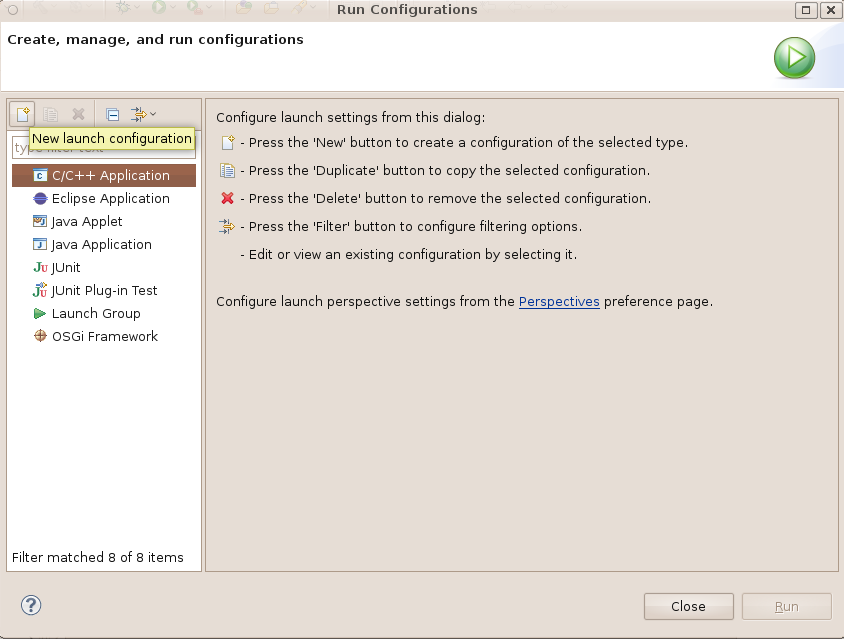
\includegraphics[width=1\textwidth]{./images/pic_compile/10_run_0.png}
%  \end{minipage}
%  \begin{minipage}[c]{.45\textwidth}
%    \centering
%    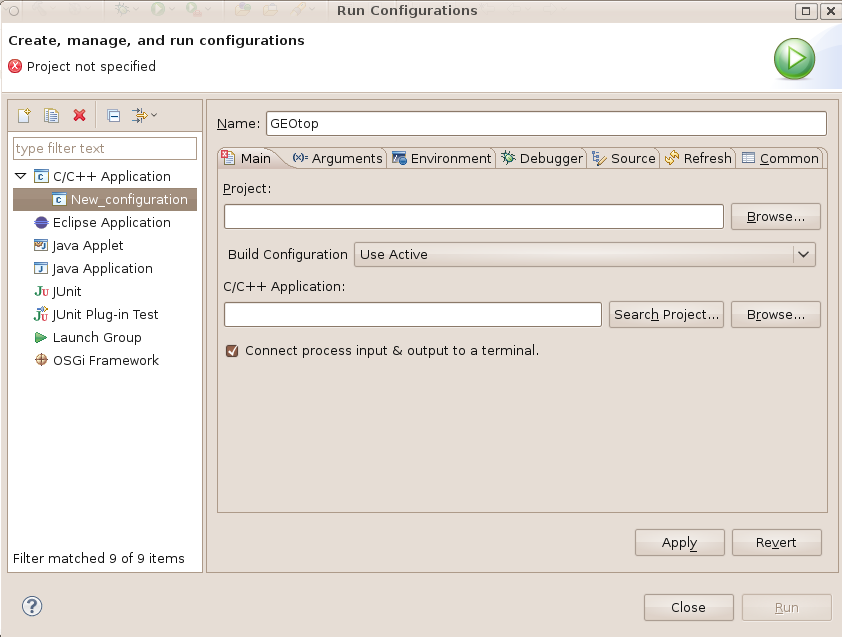
\includegraphics[width=1\textwidth]{./images/pic_compile/10_run_1.png}
%  \end{minipage}
%\end{center}
%    \textsl{\caption{SVN} \label{f:9_1}}
%\end{figure}


%\begin{figure}[!h]
%\begin{center}
%  \begin{minipage}[c]{.45\textwidth}
%    \centering
%    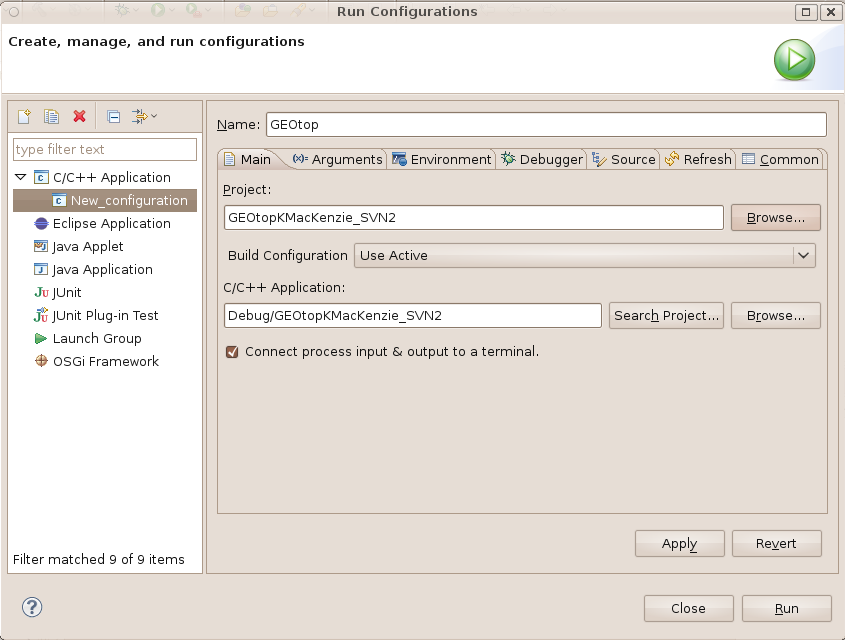
\includegraphics[width=1\textwidth]{./images/pic_compile/10_run_2.png}
%  \end{minipage}
%  \begin{minipage}[c]{.45\textwidth}
%    \centering
%    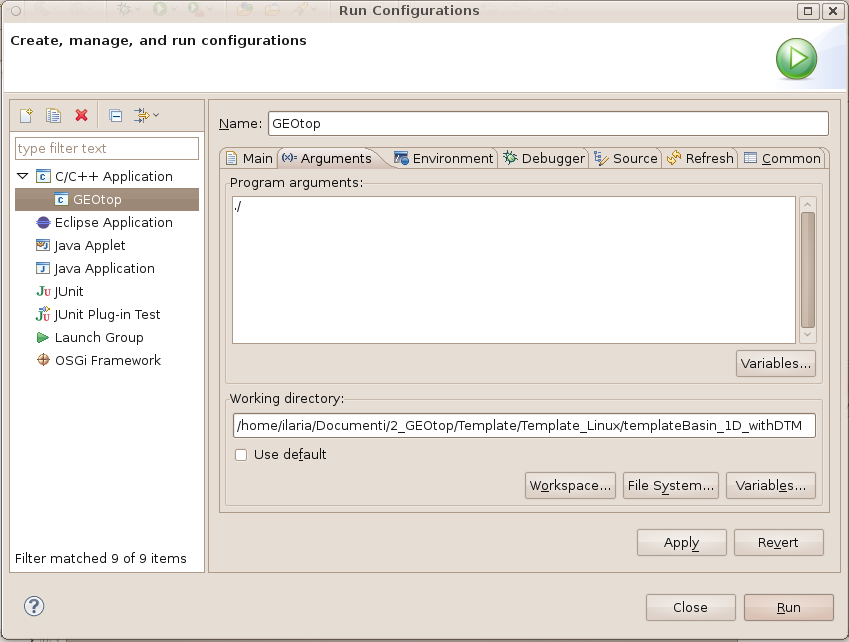
\includegraphics[width=1\textwidth]{./images/pic_compile/10_run_3.png}
%  \end{minipage}
%\end{center}
%    \textsl{\caption{SVN} \label{f:9_2}}
%\end{figure}


\chapter{I/O scheme: the keywords}

GEOtop Input/Output (I/O) scheme is based on the keyword concept. Each parameter, concerning physical processes, output personalization, domain discretization and initial/boundary condition, is described by a keyword. The keywords may be classified according to the dimension (scalar or vector), type (numerical or string) and meaning (physical or boolean), as described in the Table \ref{table_key1}.

\begin{center}
\begin{longtable}{|p {1.3 cm}|p {6 cm}|p {6. cm}|}
\hline
\textbf{} & \textbf{Scalar} & \textbf{Vector}  \\ \hline
\endfirsthead
\hline
\multicolumn{3}{| c |}{continued from previous page} \\
\hline
\textbf{} & \textbf{Scalar} & \textbf{Vector}  \\ \hline
\endhead
\hline
\multicolumn{3}{| c |}{{continued on next page}}\\ 
\hline
\endfoot
\endlastfoot
\hline
{\bf Dimension} & it refers to a single value, valid for the whole basin and during the entire simulation & it refers to more classes, layers or simulations. The vectors are composed just by numerical values (not strings).  \\ \hline
%\vspace{0.1cm} \\
%\vspace{0.1cm} & \vspace{0.1cm}  & \vspace{0.1cm} \\
\hline
& {\bf Numerical} & {\bf String}\\
\hline
{\bf Type} & it is used to assign parameters & it is used to define maps, files or headers  \\ \hline
\hline
& {\bf Physical} & {\bf Boolean}\\
\hline
{\bf Meaning} & it is used to assign physical parameters & it is used to choose or reject an option in the parameterization process  \\ \hline
\caption{Keywords classification}
\label{table_key1}
\end{longtable}
\end{center}

\noindent The keywords may be used to describe both the input data and the output personalization. In particular, the keywords identify the following types:
\begin{enumerate}
\item {\bf parameters}: they may be physical parameters, option parameters or output personalization;
\item {\bf files}: they refer to input files, containing physical parameters, and output files containing the simulation results;
\item {\bf maps}: they refer both to input maps, describing topographic features or soil characterization, and to output maps containing the simulation results;
\item {\bf tensor}: they refer both to output maps containing the simulation results in each layer, or at specified depths, producing a 3D map;
\item {\bf headers}: they refer to the column name of an input parameter or to the column name of an output result.
\end{enumerate}

\section{Keywords syntax}
The main file where the keywords are defined is {\it geotop.inpts}. In this file, each line beginning with the character ``!'' is considered a comment, and therefore the following characters in the line won't be read.
\footnotesize{
\begin{verbatim}
! THIS IS a comment
\end{verbatim}
}


\noindent In order to assign a value to the keyword, it is necessary to use the (character ``=''):
\footnotesize{
\begin{verbatim}
TimeStepEnergyAndWater = 3600
\end{verbatim}
}
\noindent This instruction orders the model to assign 3600 to the keyword {\it TimeStepEnergyAndWater}. It is possible to assign a keyword a vector of numerical values by separating the components by the character ``,''. 
\footnotesize{
\begin{verbatim}
SoilLayerThicknesses=10, 15, 30, 50
\end{verbatim}
}
\noindent This instruction assigns the keyword {\it SoilLayerThicknesses} a vector composed by 4 elements, namely: 10, 15, 30 and 50. It is not possible to assign a keyword a vector of strings.\\

\subsection{Keywords definition}

\subsubsection{Readable characters}
 The numbers, the lower and upper case letters, the characters ``.'', ``-'', ``$+$'', ``/'', ``:'', ``['', ``$\backslash$'', ``]'',  ``$\wedge$'', ``\_'', and the separator characters will be referred to as ``readable characters''. All the other characters, except for the assignation character (``$=$'') and the vector separator character (``,''), are not even read.\\

\subsubsection{Strings or numerical keywords}
The criterion used to distinguish whether an assignation is a string or numerical (be it single value or vector) is based on the {\bf first readable character} after the field separator ``='', as explained in Table \ref{table_key2}. 
As a consequence, it is not possible to assign string parameters that begin with a number or ``$+$'', ``-'', ``.'' (except ``..''), because they will be considered numerical.
Furthermore, the upper case letters are automatically converted in lower case, therefore all string keywords and parameters result to be case insensitive.

\begin{center}
\begin{longtable}{|p {4 cm}|p {4 cm}|}
\hline
\textbf{}  \textbf{First character indicating a string keyword} & \textbf{First character indicating a numerical keyword}  \\ \hline
\endfirsthead
\hline
\multicolumn{2}{| c |}{continued from previous page} \\
\hline
\textbf{}  \textbf{Characters for string} & \textbf{Character for numerical}  \\ \hline
\endhead
\hline
\multicolumn{2}{| c |}{{continued on next page}}\\ 
\hline
\endfoot
\endlastfoot
\hline
%  ``/'', ``:'', ``['', ``$\backslash$'', ``]'',``$\wedge$'', ``\_'', ``..'' , the lower and upper case letter and the numbers & numbers and the characters "." (decimal separator),``-'', ``$+$'', ``E'', and ``e''   \\ \hline
``/'' &``$+$'' \\ \hline
``:'' & ``-'' \\ \hline
``['' & ``E'' \\ \hline
``$\backslash$'' & ``e'' \\ \hline
``]'' & "." (decimal separator) \\ \hline
``$\wedge$'' & numbers \\ \hline
``\_'' &  \\ \hline
``..'' & \\ \hline
letters & \\ \hline
numbers &   \\ \hline
\caption{Character classification for strings and numerical}
\label{table_key2}
\end{longtable}
\end{center}

\noindent This means that the command lines:
\footnotesize{
\begin{verbatim}
TimeStepEnergyAndWater = 3600
\end{verbatim}
}
\noindent and:

\footnotesize{
\begin{verbatim}
TimeStepEnergyAndWater = 3 this is the first figure 6 bla bla 0 micio bau 0 polenta
\end{verbatim}
}
\noindent are actually equivalent, provided the first readable character is a number or ``$+$'', ``$-$'', ``$.$'' 
In addition, since the string are actually case insensitive, the command lines:

\footnotesize{
\begin{verbatim}
TimeStepEnergyAndWater = 3600
Time step energy and water = 3600
\end{verbatim}
}
\noindent are also equivalent.

\subsection{Dates and time}
The dates in GEOtop are considered numerical parameters and are expressed in the ``date12'' format, namely using 12 figures as DDMMYYYYhhmm, where D = day, M = month, Y = year, h = hour (in 24 hours format).
 It is necessary to use 2 figures (not only one) for the minute, hours, month, and 4 figures for the year, otherwise the date will be misunderstood. An exception is made for the day which may also be represented by one figure.
 Since within a numerical value parameter, the characters different from numbers, ``+'', ``-'', ``.'', and separators are not readable, provided they are not the first character, it is also possible to express the date12 format as DD/MM/YYYY hh:mm or DD MM YYYY hh mm, but not as DD-MM-YYYY hh:mm because "-" makes changes to the meaning of a numerical value.


\section{Keywords properties}\label{Par_keyprop}

The way the keyword are assigned is based on the following assumptions:

\paragraph{self explanatory} The keyword is generally a ``composed word'' that aims at explaining its meaning just through the words that constitute it. \\
For example the keyword: {\it TimeStepEnergyAndWater} describes the calculation time step for the energy and water balance equations. The keyword: {\it SoilLayerThicknesses} outlines the layer thickness of the soil discretization.

\paragraph{tacit}If not displayed, the parameter the keyword refers to will be initialized by the default value.
Few parameters are mandatory (it will be remarked when this is the case), while most of them are not necessary to be assigned, and the corresponding line can be skipped or commented.
The mandatory parameters are:
\begin{itemize}
\item {\it Latitude}
\item {\it Longitude}
\item integration time step for energy and water balance equation {\it TimeStepEnergyAndWater}
\item Date and time of the simulation start in date12 format {\it InitDateDDMMYYYYhhmm}
\item Date and time of the simulation end in date12 format {\it EndDateDDMMYYYYhhmm}                        
\end{itemize}

\paragraph{conservative} The keywords allow to define the output files, maps and variables to be printed.\\
Only the output variables, maps and files that have been declared by the proper keyword will be printed in order to save memory and to keep the output simple.\\
For example, if one is interested in printing the incoming, outgoing and net shortwave radiation in a simulation point, may specify:

\footnotesize{
\begin{verbatim}
!=============================================================================
!   POINT OUTPUT COLUMN NUMBER
!=============================================================================
DatePoint = 1
AirTempPoint = 2
SurfaceEBPoint = 3
SWupPoint = 4
SWinPoint = 5
SWNetPoint = 6
SoilHeatFluxPoint = 7
LWinPoint=8
LWNetPoint=9
LWupPoint=10
\end{verbatim}
}

\noindent In this way two output files will be created: ``point.txt'' (associated to the keyword {\it PointOutputFileWriteEnd}) and the file ``soilTave.txt'' associated to the keyword {\it SoilAveragedTempProfileFileWriteEnd}. The file ``point.txt'' will contain the results associated to the desired keywords at the specified column, i.e. the variable associated to the keyword {\it SWupPoint} will be printed in the column n. 2. Eventually, in case one wants to personalize the name of a output variable, it is necessary to flag the keyowrd {\it DefaultPoint=0} and then to specify the output keywords headers:

\footnotesize{
\begin{verbatim}
!=============================================================================
!   POINT OUTPUT HEADER
!=============================================================================
DefaultPoint = 0
HeaderDatePoint = "date"
HeaderSWupPoint = "SW out"
HeaderSWinPoint = "SW in"
HeaderSWNetPoint = "SW net"
\end{verbatim}
}


\noindent In case one wanted to print the average temperatures of the soil:

\footnotesize{
\begin{verbatim}
!=============================================================================
!  OUTPUT FILES
!=============================================================================
PointOutputFileWriteEnd = "point"
SoilAveragedTempProfileFileWriteEnd = "soilTave"
\end{verbatim}
}

\noindent In this case the file ``soilTave.txt'' will be produced, containing the temperatures at each layer. If one wanted to have the temperatures calculated at specified depths, one should write:
\footnotesize{
\begin{verbatim}
!=============================================================================
!  PERSONALIZED OUTPUT FILES
!=============================================================================
DefaultSoil = 0
SoilPlotDepths = 0.1, 0.5, 1, 2
\end{verbatim}
}

\indent In this case the file will contain the temperatures at 0.1, 0.5, 1.0 and 2.0 m.

\paragraph{self learning} If the keyword represents a vector of length ``$l$'' and the input consists in a vector of length ``$m$'' with $m<l$, then the successive $l-m$ elements will be initialized equal to the element ``$l$''.
For example, the keywords:

\footnotesize{
\begin{verbatim}
SoilLayerNumber=10
SoilLayerThicknesses=10, 15, 30, 50
InitSoilTemp=2
\end{verbatim}
}

\noindent are interpreted as:
\footnotesize{
\begin{verbatim}
SoilLayerNumber=10
SoilLayerThicknesses=10, 15, 30, 50, 50, 50, 50, 50, 50, 50
InitSoilTemp=2, 2, 2, 2, 2, 2, 2, 2, 2, 2
\end{verbatim}
}


\paragraph{organization} The keywords may be assigned in the {\it geotop.inpts} file or in external files defined by proper keywords, in order to ease the organization of input.  The keywords may also identify the name of files and headers to improve the output visualization.\\
For example, let us assume to run a 1D simulation on eight points whose topographical and horizon (see Par. \ref{descr_horizon}) characteristics are defined in Table \ref{table_in_topochar}.

\begin{center}
\begin{longtable}{|p {1.5 cm}|p {1.5 cm}|p {1.5 cm}|p {1.8 cm}|p {1.8 cm}|}
\hline
\textbf{Point} & \textbf{Elevation (m a.s.l.)} & \textbf{Slope ($^\circ$)} & \textbf{Aspect ($^\circ$ N)} & \textbf{Horizon file} \\ \hline
\endfirsthead
\hline
\multicolumn{5}{| c |}{continued from previous page} \\
\hline
\textbf{Point} & \textbf{Elevation (m a.s.l.)} & \textbf{Slope ($^\circ$)} & \textbf{Aspect ($^\circ$ N)} \textbf{Horizon file} \\ \hline
\endhead
\hline
\multicolumn{5}{| c |}{{continued on next page}}\\ 
\hline
\endfoot
\endlastfoot
\hline
1 & 1600 & 10 & 0 & 1  \\ \hline
2 & 2100 & 10 & 0 & 2  \\ \hline
3 & 1600 & 30 & 0 & 1  \\ \hline
4 & 2100 & 30 & 0 & 2  \\ \hline
5 & 1600 & 10 & 180 & 1  \\ \hline
6 & 2100 & 10 & 180 & 2  \\ \hline
7 & 1600 & 30 & 180 & 1  \\ \hline
8 & 2100 & 30 & 180 & 2  \\ \hline
\caption{Topographical characteristics of the simulation points}
\label{table_in_topochar}
\end{longtable}
\end{center}

\noindent In order to provide these characteristics, one has two options. In the first option, one uses only the {\it geotop.inpts} file:
\footnotesize{
\begin{verbatim}
HorizonPointFile= "horfile"
HeaderHorizonAngle = "azi"
HeaderHorizonHeight = "hang"
PointElevation = 1600, 2100, 1600, 2100, 1600, 2100, 1600, 2100
PointSlope = 10, 30, 10, 30, 10, 30, 10, 30
PointAspect = 0, 180, 0, 180, 0, 180, 0, 180
PointHorizon = 1, 2, 1, 2, 1, 2, 1, 2
\end{verbatim}
}

\noindent where the {\it HorizonPointFile} becomes (see Table \ref{azh}):
\footnotesize{
\begin{verbatim}
azi, hang
45, 0
135, 10
225, 30
315, 5
\end{verbatim}
}


\noindent Alternatively, in order to ease the comprehension, especially when the number of simulation points is high, one could define an external file ({\it PointFile}) containing the features of the points, where the name of the columns has been defined in {\it geotop.inpts} in the proper ``header'' keywords. This would result in:

\footnotesize{
\begin{verbatim}
HorizonPointFile = "horfile"
PointFile = "listpoints"
HeaderPointElevation = "ele"
HeaderPointSlope = "slp"
HeaderPointAspect = "asp"
HeaderPointHorizon = "hor"
HeaderHorizonAngle="azi"
HeaderHorizonHeight="hang"
\end{verbatim}
}

\noindent and the correspondent {\it PointFile} would result in:
\footnotesize{
\begin{verbatim}
ID, ele, slp, asp, hor
1, 1600, 10, 0, 1
2, 2100, 30, 180, 2
3, 1600, 10, 0, 1
4, 2100, 30, 180, 2
5, 1600, 10, 0, 1
6, 2100, 30, 180, 2
7, 1600, 10, 0, 1
8, 2100, 30, 180, 2
\end{verbatim}
}



\chapter{1D: domain definition and characterization}



As pointed out in Fig. \ref{Fig_sim_flowchart}, the 1D simulation may defined in two ways: 
\begin{enumerate}
\item with maps: in this case the user must provide also the topographical maps together with the land cover, the soil type and, if present, the initial conditions maps. Furthermore, the user must give in input also the coordinates of the simulation points (see Fig. \ref{grid3Dversante_points} and \ref{Fig_meteoST1}). The model automatically extrapolates the information on the give points through the provided maps;
\item without maps: in this case, the user must provide all the necessary information about the topography, land cover and soil type of the simulation points.
\end{enumerate}

\noindent In both cases the domain discretization along the Z coordinate (Fig. \ref{Fig_discr3d} on the right) must be properly defined as described in Table \ref{domain_Zcoord}.

\begin{center}
\begin{longtable}{|p {3.5 cm}|p {4.7 cm}|p {1. cm}|p{0.8 cm}|p{1.4 cm}|p{0.8 cm}|p{1.3 cm}|}
\hline
\textbf{Keyword} & \textbf{Description} & \textbf{M. U.} & \textbf{range} & \textbf{Default Value} & \textbf{Sca / Vec} & \textbf{Str / Num / Opt} \\ \hline
\endfirsthead
\hline
\multicolumn{7}{| c |}{continued from previous page} \\
\hline
\textbf{Keyword} & \textbf{Description} & \textbf{M. U.} & \textbf{range} & \textbf{Default Value} & \textbf{Sca / Vec} & \textbf{Str / Num / Opt} \\ \hline
\endhead
\hline
\multicolumn{7}{| c |}{{continued on next page}}\\ 
\hline
\endfoot
\endlastfoot
\hline
%PointSoilType & Soil type of the simulation point & - &  & NA & vec & num \\ \hline
SoilLayerThicknesses & vector defining the thickness of the various soil layers. If not present, a column of 5 layers 100 mm thick will be assumed & mm &  & 100 & vec & num \\ \hline
SoilLayerNumber & number of soil layers (is calculated after the number of components of the vector SoilLayerNumber) & - &  & 5 & sca & num \\ \hline
\caption{Keywords of parameters referred to soil layer}
\label{domain_Zcoord}
\end{longtable}
\end{center}

\section{Without maps}

\subsubsection{Parameters}
\begin{center}
\begin{longtable}{|p {5.5 cm}|p {3. cm}|p {1.2 cm}|p{1.0 cm}|p{1.2 cm}|p{0.8 cm}|p{1. cm}|}
\hline
\textbf{Keyword} & \textbf{Description} & \textbf{M. U.} & \textbf{range} & \textbf{Default Value} & \textbf{Sca / Vec} & \textbf{Log / Num} \\ \hline
\endfirsthead
\hline
\multicolumn{7}{| c |}{continued from previous page} \\
\hline
\textbf{Keyword} & \textbf{Description} & \textbf{M. U.} & \textbf{range} & \textbf{Default Value} & \textbf{Sca / Vec} & \textbf{Log / Num} \\ \hline
\endhead
\hline
\multicolumn{7}{| c |}{{continued on next page}}\\ 
\hline
\endfoot
\endlastfoot
\hline
PointLandCoverType \index{PointLandCoverType} & Land Cover type of the simulation point & - &  & NA & vec & num \\ \hline
PointSoilType \index{PointSoilType} & Soil type of the simulation point & - &  & NA & vec & num \\ \hline
PointElevation \index{PointElevation} & elevation of the point of simulation & m a.s.l. &  & NA & vec & num \\ \hline
PointSlope \index{PointSlope} & Slope steepness of the simulation point & degree &  & NA & vec & num \\ \hline
PointAspect \index{PointAspect} & Aspect of the simulation point & degree &  & NA & vec & num \\ \hline
PointSkyViewFactor \index{PointSkyViewFactor}& Sky View Factor of the simulation point & - &  & NA & vec & num \\ \hline
PointCurvatureNorthSouthDirection \index{PointCurvatureNorthSouthDirection} & N-S curvature of the simulation point & m$^{-1}$ &  & NA & vec & num \\ \hline
PointCurvatureWestEastDirection \index{PointCurvatureWestEastDirection} & W-E curvature of the simulation point & m$^{-1}$ &  & NA & vec & num \\ \hline
PointCurvatureNorthwestSoutheastDirection \index{PointCurvatureNorthwestSoutheastDirection}& N-W curvature of the simulation point & m$^{-1}$ &  & NA & vec & num \\ \hline
PointCurvatureNortheastSouthwestDirection \index{PointCurvatureNortheastSouthwestDirection} & N-E curvature of the simulation point & m$^{-1}$ &  & NA & vec & num \\ \hline
PointDrainageLateralDistance \index{PointDrainageLateralDistance} & Lateral Drainage distance of the simulation point & m &  & NA & vec & num \\ \hline
PointLatitude \index{PointLatitude} & Latitude of the simulation point & degree &  & NA & vec & num \\ \hline
PointLongitude \index{PointLongitude} & Longitude of the simulation point & degree &  & NA & vec & num \\ \hline
PointHorizon \index{PointHorizon} & number of the HorizonPointFile that describes the horizon of the simulation point & - &  & NA & vec & num \\ \hline
\caption {Keywords of topographical, land cover and soil type characteristics that may be set in geotop.inpts. Each parameter may be give in input as a vector, each component representing a point. Otherwise the characteristics may be summarized in the file PointFile, each value corresponding to the proper header defined in Table \ref{headers_topo_par1D}. }
\label{topo_par1d_topo}
\end{longtable}
\end{center}


\subsubsection{Files}

\begin{center}
\begin{longtable}{|p {2.5 cm}|p {8.5 cm}|p {1 cm}|p {1 cm}|}
\hline
\textbf{Keyword} & \textbf{Description}  \\ \hline
\endfirsthead
\hline
\multicolumn{4}{| c |}{continued from previous page} \\
\hline
\textbf{Keyword} & \textbf{Description}  \\ \hline
\endhead
\hline
\multicolumn{4}{| c |}{{continued on next page}}\\ 
\hline
\endfoot
\endlastfoot
\hline
PointFile \index{PointFile} & name of the file providing the properties for the simulation point  \\ \hline
HorizonPointFile \index{HorizonPointFile} & name of the file providing the horizon of the simulation point  \\ \hline
\caption{Keywords of files related to soil/rock spatial characterization for 1D simulation}
\label{key1D_data}
\end{longtable}
\end{center}

\subsubsection{Headers}

\begin{center}
\begin{longtable}{|p {6.5 cm}|p {6 cm}|p {2 cm}|p {1 cm}|}
\hline
\textbf{Keyword} & \textbf{Description} & \textbf{Associated file}  \\ \hline
\endfirsthead
\hline
\multicolumn{4}{| c |}{continued from previous page} \\
\hline
\textbf{Keyword} & \textbf{Description} & \textbf{Associated file}  \\ \hline
\endhead
\hline
\multicolumn{4}{| c |}{{continued on next page}}\\ 
\hline
\endfoot
\endlastfoot
\hline
HeaderHorizonAngle \index{HeaderHorizonAngle} & String representing the header of the column HorizonAngle of the HorizonPoint and HorizonMeteoStation files & HorizonPoint / HorizonMeteoStation  \\ \hline
HeaderHorizonHeight \index{HeaderHorizonHeight} & String representing the header of the column HorizonHeight of the HorizonPoint and HorizonMeteoStation files & HorizonPoint / HorizonMeteoStation  \\ \hline
HeaderPointElevation \index{HeaderPointElevation} & column name in the file PointFile for the elevation of the point & PointFile  \\ \hline
HeaderPointSlope \index{HeaderPointSlope} & column name in the file PointFile for the slope steepness of the point & PointFile  \\ \hline
HeaderPointAspect \index{HeaderPointAspect} & column name in the file PointFile for the aspect of the point & PointFile  \\ \hline
HeaderPointSkyViewFactor \index{HeaderPointSkyViewFactor} & column name in the file PointFile for the sky view factor of the point & PointFile  \\ \hline
HeaderPointCurvatureNorthSouthDirection \index{HeaderPointCurvatureNorthSouthDirection} & column name in the file PointFile for the N-S curvature of the point & PointFile  \\ \hline
HeaderPointCurvatureWestEastDirection \index{HeaderPointCurvatureWestEastDirection} & column name in the file PointFile for the E-W curvature of the point & PointFile  \\ \hline
HeaderPointCurvatureNorthwestSoutheastDirection \index{HeaderPointCurvatureNorthwestSoutheastDirection} & column name in the file PointFile for the NW-SE curvature of the point & PointFile  \\ \hline
HeaderPointCurvatureNortheastSouthwestDirection \index{HeaderPointCurvatureNortheastSouthwestDirection} & column name in the file PointFile for the NE-SW curvature of the point & PointFile  \\ \hline
HeaderPointDrainageLateralDistance \index{HeaderPointDrainageLateralDistance} & column name in the file PointFile for the distance of lateral drainage & PointFile  \\ \hline
HeaderPointHorizon \index{HeaderPointHorizon} & column name in the file PointFile that provides the number of the HorizonPointFile that describes the horizon of the simulation point & PointFile  \\ \hline
HeaderPointLatitude \index{HeaderPointLatitude} & column name in the file PointFile for the latitude of the point & PointFile  \\ \hline
HeaderPointLongitude \index{HeaderPointLongitude} & column name in the file PointFile for the longitude of the point & PointFile  \\ \hline
HeaderPointID \index{HeaderPointID} & column name in the file PointFile for the identification ID of the point & PointFile  \\ \hline
HeaderCoordinatePointX \index{HeaderCoordinatePointX} & column name in the file PointFile for the x coordinate of the point & PointFile  \\ \hline
HeaderCoordinatePointY \index{HeaderCoordinatePointY} & column name in the file PointFile for the y coordinate of the point & PointFile  \\ \hline
\caption{Keywords of headers that specify the soil/rock spatial characterization for 1D simulation}
\label{headers_topo_par1D}
\end{longtable}
\end{center}






\section{With maps}

\subsubsection{Maps}

\begin{center}
\begin{longtable}{|p {3.5 cm}|p {6.5 cm}|p {3 cm}|p {4 cm}|}
\hline
\textbf{Keyword} & \textbf{Description}  \\ \hline
\endfirsthead
\hline
\multicolumn{4}{| c |}{continued from previous page} \\
\hline
\textbf{Keyword} & \textbf{Description}  \\ \hline
\endhead
\hline
\multicolumn{4}{| c |}{{continued on next page}}\\ 
\hline
\endfoot
\endlastfoot
\hline
DemFile \index{DemFile} & name of the file providing the DEM map  \\ \hline
SkyViewFactorMapFile \index{SkyViewFactorMapFile}& name of the file providing the sky view factor map  \\ \hline
SlopeMapFile \index{SlopeMapFile} & name of the file providing the slope steepness map  \\ \hline
RiverNetwork \index{RiverNetwork} & name of the file providing the river network map  \\ \hline
AspectMapFile \index{AspectMapFile} & name of the file providing the aspect map  \\ \hline
CurvaturesMapFile \index{CurvaturesMapFile} & name of the file providing the curvature map  \\ \hline
%BedrockDepthMapFile & name of the file providing the bedrock depth map  \\ \hline
LandCoverMapFile \index{LandCoverMapFile} & name of the file providing the land cover map  \\ \hline
SoilMapFile \index{SoilMapFile} & name of the file providing the soil map  \\ \hline
\caption{Keywords of input file related to the domain}
\label{Input_top_1D_withoutmaps}
\end{longtable}
\end{center}

\subsubsection{Files}

\begin{center}
\begin{longtable}{|p {2.5 cm}|p {8.5 cm}|p {1 cm}|p {1 cm}|}
\hline
\textbf{Keyword} & \textbf{Description}  \\ \hline
\endfirsthead
\hline
\multicolumn{4}{| c |}{continued from previous page} \\
\hline
\textbf{Keyword} & \textbf{Description}  \\ \hline
\endhead
\hline
\multicolumn{4}{| c |}{{continued on next page}}\\ 
\hline
\endfoot
\endlastfoot
\hline
PointFile \index{PointFile} & name of the file providing the properties for the simulation point  \\ \hline
\caption{Keyword of the file related to the spatial characterization of soil/rock properties. The parameters identified by the row index represent the value corresponding to the SoilMapFile map.}
\label{key3D_data_ii}
\end{longtable}
\end{center}


\subsubsection{Parameters}
\begin{center}
\begin{longtable}{|p {2.2 cm}|p {4.2 cm}|p {2.7 cm}|p{1.0 cm}|p{1.2 cm}|p{0.8 cm}|p{1. cm}|}
\hline
\textbf{Keyword} & \textbf{Description} & \textbf{M. U.} & \textbf{range} & \textbf{Default Value} & \textbf{Sca / Vec} & \textbf{Log / Num} \\ \hline
\endfirsthead
\hline
\multicolumn{7}{| c |}{continued from previous page} \\
\hline
\textbf{Keyword} & \textbf{Description} & \textbf{M. U.} & \textbf{range} & \textbf{Default Value} & \textbf{Sca / Vec} & \textbf{Log / Num} \\ \hline
\endhead
\hline
\multicolumn{7}{| c |}{{continued on next page}}\\ 
\hline
\endfoot
\endlastfoot
\hline
PointID \index{PointID}& identification code for the point of simulation &  &  & NA & vec & num \\ \hline
CoordinatePointX \index{CoordinatePointX}& coordinate X if PixelCoordinates is 1, number of row of the matrix if PixelCoordinates is 0 & m (according to the geographical projection of the maps) &  & NA & vec & num \\ \hline
CoordinatePointY \index{CoordinatePointY} & coordinate Y if PixelCoordinates is 1, number of column of the matrix if PixelCoordinates is 1 & m (according to the geographical projection of the maps) &  & NA & vec & num \\ \hline
Latitude \index{Latitude} & Average latitude of the basin, positive means north, negative means south & degree & -90, 90 & 45 & sca & num \\ \hline
Longitude \index{Longitude} & Average longitude of the basin, eastwards from 0 meridiane & degree & 0, 180 & 0 & sca & num \\ \hline
\caption{Keywords of point characterization for the choice of points where to perform a 1D simulation}
\label{topo_par1d_withmaps}
\end{longtable}
\end{center}

\subsubsection{Headers}

\begin{center}
\begin{longtable}{|p {4.15 cm}|p {8 cm}|p {2 cm}|p {1 cm}|}
\hline
\textbf{Keyword} & \textbf{Description} & \textbf{Associated file}  \\ \hline
\endfirsthead
\hline
\multicolumn{4}{| c |}{continued from previous page} \\
\hline
\textbf{Keyword} & \textbf{Description} & \textbf{Associated file}  \\ \hline
\endhead
\hline
\multicolumn{4}{| c |}{{continued on next page}}\\ 
\hline
\endfoot
\endlastfoot
\hline
HeaderPointID \index{HeaderPointID}& column name in the file PointFile for the identification ID of the point & PointFile  \\ \hline
HeaderCoordinatePointX \index{HeaderCoordinatePointX} & column name in the file PointFile for the x coordinate of the point & PointFile  \\ \hline
HeaderCoordinatePointY \index{HeaderCoordinatePointY}& column name in the file PointFile for the y coordinate of the point & PointFile  \\ \hline
\caption{Keywords of headers that specify the soil/rock spatial characterization for 1D simulation}
\label{headers_topo_par1D}
\end{longtable}
\end{center}



\chapter{3D: domain definition and characterization}



\section{Planar domain definition}


\begin{center}
\begin{longtable}{|p {3.5 cm}|p {6.5 cm}|p {3 cm}|p {4 cm}|}
\hline
\textbf{Keyword} & \textbf{Description}  \\ \hline
\endfirsthead
\hline
\multicolumn{4}{| c |}{continued from previous page} \\
\hline
\textbf{Keyword} & \textbf{Description}  \\ \hline
\endhead
\hline
\multicolumn{4}{| c |}{{continued on next page}}\\ 
\hline
\endfoot
\endlastfoot
\hline
DemFile & name of the file providing the DEM map  \\ \hline
LandCoverMapFile & name of the file providing the land cover map  \\ \hline
\caption{Keywords of input file related to the domain}
\label{input_file}
\end{longtable}
\end{center}


\section{Z-coordinate domain definition}

\begin{center}
\begin{longtable}{|p {3.5 cm}|p {4.7 cm}|p {1. cm}|p{0.8 cm}|p{1.4 cm}|p{0.8 cm}|p{1.3 cm}|}
\hline
\textbf{Keyword} & \textbf{Description} & \textbf{M. U.} & \textbf{range} & \textbf{Default Value} & \textbf{Sca / Vec} & \textbf{Str / Num / Opt} \\ \hline
\endfirsthead
\hline
\multicolumn{7}{| c |}{continued from previous page} \\
\hline
\textbf{Keyword} & \textbf{Description} & \textbf{M. U.} & \textbf{range} & \textbf{Default Value} & \textbf{Sca / Vec} & \textbf{Str / Num / Opt} \\ \hline
\endhead
\hline
\multicolumn{7}{| c |}{{continued on next page}}\\ 
\hline
\endfoot
\endlastfoot
\hline
%PointSoilType & Soil type of the simulation point & - &  & NA & vec & num \\ \hline
SoilLayerThicknesses \index{SoilLayerThicknesses} & vector defining the thickness of the various soil layers. If not present, a column of 5 layers 100 mm thick will be assumed & mm &  & 100 & vec & num \\ \hline
SoilLayerNumber \index{SoilLayerNumber} & number of soil layers (is calculated after the number of components of the vector SoilLayerNumber) & - &  & 5 & sca & num \\ \hline
\caption{Keywords of  parameters referred to soil layer}
\label{domain_parameters1D_numeric}
\end{longtable}
\end{center}

\section{Topographical characterization}

\begin{center}
\begin{longtable}{|p {3.5 cm}|p {7 cm}|p {1 cm}|p {1 cm}|}
\hline
\textbf{Keyword} & \textbf{Description}  \\ \hline
\endfirsthead
\hline
\multicolumn{4}{| c |}{continued from previous page} \\
\hline
\textbf{Keyword} & \textbf{Description}  \\ \hline
\endhead
\hline
\multicolumn{4}{| c |}{{continued on next page}}\\ 
\hline
\endfoot
\endlastfoot
\hline
SkyViewFactorMapFile \index{SkyViewFactorMapFile}& name of the file providing the sky view factor map  \\ \hline
SlopeMapFile \index{SlopeMapFile} & name of the file providing the slope steepness map  \\ \hline
RiverNetwork \index{RiverNetwork}& name of the file providing the river network map  \\ \hline
AspectMapFile \index{AspectMapFile} & name of the file providing the aspect map  \\ \hline
CurvaturesMapFile \index{CurvaturesMapFile} & name of the file providing the curvature map  \\ \hline
BedrockDepthMapFile \index{BedrockDepthMapFile}& name of the file providing the bedrock depth map  \\ \hline
\caption{Keywords of input maps necessary to launch the 3D simulation}
\label{table_3D_topochar}
\end{longtable}
\end{center}

\section{Land cover and soil depth characterization}

\begin{center}
\begin{longtable}{|p {3.5 cm}|p {7 cm}|p {1 cm}|p {1 cm}|}
\hline
\textbf{Keyword} & \textbf{Description}  \\ \hline
\endfirsthead
\hline
\multicolumn{4}{| c |}{continued from previous page} \\
\hline
\textbf{Keyword} & \textbf{Description}  \\ \hline
\endhead
\hline
\multicolumn{4}{| c |}{{continued on next page}}\\ 
\hline
\endfoot
\endlastfoot
\hline
LandCoverMapFile \index{LandCoverMapFile} & name of the file providing the land cover map  \\ \hline
SoilMapFile \index{SoilMapFile}& name of the file providing the soil map  \\ \hline
\caption{Keywords of input maps necessary to launch the 3D simulation}
\label{table_3D_landchar}
\end{longtable}
\end{center}



\noindent Each land cover type may be characterized by parameters that define the influence on vegetation, soil surface and snow. Each soil type may be further described in the file {\it PointFile} (see Table \ref{table_3D_landchar_file}) where each row index represents the value corresponding to the {\it SoilMapFile} map.

\begin{center}
\begin{longtable}{|p {2.5 cm}|p {8.5 cm}|p {1 cm}|p {1 cm}|}
\hline
\textbf{Keyword} & \textbf{Description}  \\ \hline
\endfirsthead
\hline
\multicolumn{4}{| c |}{continued from previous page} \\
\hline
\textbf{Keyword} & \textbf{Description}  \\ \hline
\endhead
\hline
\multicolumn{4}{| c |}{{continued on next page}}\\ 
\hline
\endfoot
\endlastfoot
\hline
PointFile \index{PointFile}& name of the file providing the properties for the simulation point  \\ \hline
\caption{Keyword of the file related to the spatial characterization of soil/rock properties. The parameters identified by the row index represent the value corresponding to the SoilMapFile map.}
\label{table_3D_landchar_file}
\end{longtable}
\end{center}

\noindent It is also requested to provide a definition of the average latitude and longitude of the domain area, as specified in Table \ref{topo_par3d_gen}.

\begin{center}
\begin{longtable}{|p {2.3 cm}|p {6. cm}|p {1.5 cm}|p{1.0 cm}|p{1.2 cm}|p{0.8 cm}|p{1. cm}|}
\hline
\textbf{Keyword} & \textbf{Description} & \textbf{M. U.} & \textbf{range} & \textbf{Default Value} & \textbf{Sca / Vec} & \textbf{Log / Num} \\ \hline
\endfirsthead
\hline
\multicolumn{7}{| c |}{continued from previous page} \\
\hline
\textbf{Keyword} & \textbf{Description} & \textbf{M. U.} & \textbf{range} & \textbf{Default Value} & \textbf{Sca / Vec} & \textbf{Log / Num} \\ \hline
\endhead
\hline
\multicolumn{7}{| c |}{{continued on next page}}\\ 
\hline
\endfoot
\endlastfoot
\hline
Latitude \index{Latitude}& Average latitude of the basin, positive means north, negative means south & degree & -90, 90 & 45 & sca & num \\ \hline
Longitude \index{Longitude} & Average longitude of the basin, eastwards from 0 meridiane & degree & 0, 180 & 0 & sca & num \\ \hline
\caption {Keyword of parameters describing the point characterization for 3D simulations}
\label{topo_par3d_gen}
\end{longtable}
\end{center}


\section{Output}

It is possible to define some points where to obtain output information, as described in Par. \ref{par:focusPoints}. The parameters and headers to provide are specified in Table \ref{header_soilrock3D} and \ref{topo_par3d_gen} respectively.


\begin{center}
\begin{longtable}{|p {3.5 cm}|p {4.5 cm}|p {2.5 cm}|p {4 cm}|}
\hline
\textbf{Keyword} & \textbf{Description} & \textbf{Associated file}  \\ \hline
\endfirsthead
\hline
\multicolumn{4}{| c |}{continued from previous page} \\
\hline
\textbf{Keyword} & \textbf{Description} & \textbf{Associated file}  \\ \hline
\endhead
\hline
\multicolumn{4}{| c |}{{continued on next page}}\\ 
\hline
\endfoot
\endlastfoot
\hline
HeaderPointID \index{HeaderPointID}& column name in the file PointFile for the identification ID of the point & PointFile  \\ \hline
HeaderCoordinatePointX \index{HeaderCoordinatePointX} & column name in the file PointFile for the x coordinate of the point & PointFile  \\ \hline
HeaderCoordinatePointY \index{HeaderCoordinatePointY} & column name in the file PointFile for the y coordinate of the point & PointFile  \\ \hline
\caption{Keywords of header that specify the soil/rock spatial characterization for 3D simulation }
\label{header_soilrock3D}
\end{longtable}
\end{center}


\begin{center}
\begin{longtable}{|p {2.2 cm}|p {4.2 cm}|p {2.7 cm}|p{1.0 cm}|p{1.2 cm}|p{0.8 cm}|p{1. cm}|}
\hline
\textbf{Keyword} & \textbf{Description} & \textbf{M. U.} & \textbf{range} & \textbf{Default Value} & \textbf{Sca / Vec} & \textbf{Log / Num} \\ \hline
\endfirsthead
\hline
\multicolumn{7}{| c |}{continued from previous page} \\
\hline
\textbf{Keyword} & \textbf{Description} & \textbf{M. U.} & \textbf{range} & \textbf{Default Value} & \textbf{Sca / Vec} & \textbf{Log / Num} \\ \hline
\endhead
\hline
\multicolumn{7}{| c |}{{continued on next page}}\\ 
\hline
\endfoot
\endlastfoot
\hline
PointID \index{PointID}& identification code for the point of simulation &  &  & NA & vec & num \\ \hline
CoordinatePointX \index{CoordinatePointX} & coordinate X if PixelCoordinates is 1, number of row of the matrix if PixelCoordinates is 0 & m (according to the geographical projection of the maps) &  & NA & vec & num \\ \hline
CoordinatePointY \index{CoordinatePointY}& coordinate Y if PixelCoordinates is 1, number of column of the matrix if PixelCoordinates is 1 & m (according to the geographical projection of the maps) &  & NA & vec & num \\ \hline
\caption{Keywords of point characterization for the choice of point outputs in 3D simulations}
\label{topo_par3d_gen}
\end{longtable}
\end{center}




%\begin{figure}[h!]
%\begin{center}
%  \begin{minipage}[c]{.65\textwidth}
%    \centering
%    \includegraphics[width=1\textwidth]{./images/pic_spatchar/discretizzazione_3d.pdf}
%  \end{minipage}%
%  \hspace{10mm}%
%  \begin{minipage}[c]{.25\textwidth}
%    \centering
%    \includegraphics[width=1\textwidth]{./images/pic_spatchar/soil_stratigraphy_basin.pdf}
%  \end{minipage}
%\end{center}
%\textsl{\caption{Soil stratigraphy}\label{ww}}
%\end{figure}



\chapter{General features}

\section{Input}

\subsection{File}
\begin{center}
\begin{longtable}{|p {4.2 cm}|p {7 cm}|p {2 cm}|p {1.5 cm}|}
\hline
\textbf{Keyword} & \textbf{Description}  \\ \hline
\endfirsthead
\hline
\multicolumn{4}{| c |}{continued from previous page} \\
\hline
\textbf{Keyword} & \textbf{Description}  \\ \hline
\endhead
\hline
\multicolumn{4}{| c |}{{continued on next page}}\\ 
\hline
\endfoot
\endlastfoot
\hline
TimeStepsFile \index{TimeStepsFile} & name of the file providing the integration time steps \\ \hline
\caption{Keyword of file related to general input}
\label{gen_file}
\end{longtable}
\end{center}


\subsection{Parameters}

\begin{center}
\begin{longtable}{|p {3.8 cm}|p {4.2 cm}|p {1 cm}|p{1.3 cm}|p{1. cm}|p{0.8 cm}|p{0.8 cm}|}
\hline
\textbf{Keyword} & \textbf{Description} & \textbf{M. U.} & \textbf{range} & \textbf{Default Value} & \textbf{Sca / Vec} & \textbf{Log / Num} \\ \hline
\endfirsthead
\hline
\multicolumn{7}{| c |}{continued from previous page} \\
\hline
\textbf{Keyword} & \textbf{Description} & \textbf{M. U.} & \textbf{range} & \textbf{Default Value} & \textbf{Sca / Vec} & \textbf{Log / Num} \\ \hline
\endhead
\hline
\multicolumn{7}{| c |}{{continued on next page}}\\ 
\hline
\endfoot
\endlastfoot
\hline
FlagSkyViewFactor \index{FlagSkyViewFactor} & If not present, the sky view factor can be calculated (=1), or just be considered only equal to 1 (=0) & - & 0, 1 & 0 & sca & opt \\ \hline
TimeStepEnergyAndWater \index{TimeStepEnergyAndWater} & Integrations time step [s] for energy and water balance equation (mandatory) & s & 0, inf & NA & vec & num \\ \hline
InitDateDDMMYYYYhhmm \index{InitDateDDMMYYYYhhmm} & Date and time of the simulation start in date12 format (mandatory) & format DDMMYYhhmm & 01/01/1800 00:00, 01/01/2500 00:00 & NA & vec & str \\ \hline
EndDateDDMMYYYYhhmm \index{EndDateDDMMYYYYhhmm} & Date and time of the simulation start in date12 format (mandatory) & format DDMMYYhhmm & 01/01/1800 00:00, 01/01/2500 00:00 & NA & vec & str \\ \hline
NumSimulationTimes \index{NumSimulationTimes} & How many times the simulation is run (if $>$1, it uses the final condition as initial conditions of the new simulation) & - & 0, inf & 1 & vec & num \\ \hline
StandardTimeSimulation \index{StandardTimeSimulation} & Standard time to which all the output data are referred (difference respect UMT, in hours): GMT + x [h] & h & 0, 12 & 0 & sca & num \\ \hline
PointSim \index{PointSim} & Point simulation (=1), distributed simulation (=0) & - & 0, 1 & 0 & sca & opt \\ \hline
RecoverSim \index{RecoverSim} & Simulation recovered (n=number of saving point you want to start from), otherwise (=0) & - & 0, max saving points & 0 & sca & opt \\ \hline
WaterBalance \index{WaterBalance} & Activate water balance (Yes=1, No=0) & - &  & 0 & sca & opt \\ \hline
EnergyBalance \index{EnergyBalance} & Activate energy balance (Yes=1, No=0) &  &  & 0 & sca & opt \\ \hline
PixelCoordinates \index{PixelCoordinates} & Write 1 IF ALL point coordinates are in format (East, North) in meter, or if in format row and colums (r,c) of the dem map & - &  & 1 & sca & opt \\ \hline
SavingPoints \index{SavingPoints} &  & - &max saving points  & NA & vec & num \\ \hline
SoilLayerTypes \index{SoilLayerTypes} & Number of types of soil types, corresponding to different soil stratigraphies & - &  & 1 & sca & num \\ \hline
DefaultSoilTypeLand \index{DefaultSoilTypeLand} & given a multiple number of type of soil, this relates to the default given to the land type & - &  & 1 & sca & num \\ \hline
DefaultSoilTypeChannel \index{DefaultSoilTypeChannel} & given a multiple number of type of soil, this relates to the default given to the channel type & - &  & 1 & sca & num \\ \hline
\caption{Keywords for the general parameters settable in geotop.inpts}
\label{general_numeric}
\end{longtable}
\end{center}


\section{Output}

\subsection{Maps parameters}

\begin{center}
\begin{longtable}{|p {3.4 cm}|p {4.5 cm}|p {1 cm}|p{1.3 cm}|p{1. cm}|p{0.8 cm}|p{0.8 cm}|}
\hline
\textbf{Keyword} & \textbf{Description} & \textbf{M. U.} & \textbf{range} & \textbf{Default Value} & \textbf{Sca / Vec} & \textbf{Log / Num} \\ \hline
\endfirsthead
\hline
\multicolumn{7}{| c |}{continued from previous page} \\
\hline
\textbf{Keyword} & \textbf{Description} & \textbf{M. U.} & \textbf{range} & \textbf{Default Value} & \textbf{Sca / Vec} & \textbf{Log / Num} \\ \hline
\endhead
\hline
\multicolumn{7}{| c |}{{continued on next page}}\\ 
\hline
\endfoot
\endlastfoot
\hline
FormatOutputMaps \index{FormatOutputMaps}& Format of the output maps (=2 grass ascii, =3 esri ascii) & - & 2, 3 & 3 & sca & opt \\ \hline
\caption{Keywords of general parameters regarding output options that may be set in geotop.inpts}
\label{gen_out_par}
\end{longtable}
\end{center}
%%%%%%%%%%%%%%%%%%%%%%%%%%%%%%%%%%%%%%%%%%%%%%%%%%%%%%%%%%%%%%%
\chapter{Meteo Forcing}\label{}
%%%%%%%%%%%%%%%%%%%%%%%%%%%%%%%%%%%%%%%%%%%%%%%%%%%%%%%%%%%%%%%

%%%%%%%%%%%%%%%%%%%%%%%%%%%%%%%%%%%%%%%%%%%%%%%%%%%%%%%%%%%%%%%
\section{Input}
%%%%%%%%%%%%%%%%%%%%%%%%%%%%%%%%%%%%%%%%%%%%%%%%%%%%%%%%%%%%%%%


\subsection{Files}

\begin{center}
\begin{longtable}{|p {4.2 cm}|p {8 cm}|}
\hline
\textbf{Keyword} & \textbf{Description}  \\ \hline
\endfirsthead
\hline
\multicolumn{2}{| c |}{continued from previous page} \\
\hline
\textbf{Keyword} & \textbf{Description}  \\ \hline
\endhead
\hline
\multicolumn{2}{| c |}{{continued on next page}}\\ 
\hline
\endfoot
\endlastfoot
\hline
MeteoFile \index{MeteoFile} & name of the file providing the meteo forcing data  \\ \hline
MeteoStationsListFile \index{MeteoStationsListFile} & name of the file providing the Meteo Station list  \\ \hline
LapseRateFile \index{LapseRateFile} & name of the file providing the Lapse rate  \\ \hline
HorizonMeteoStationFile \index{HorizonMeteoStationFile} & name of the file providing the horizon of the meteo station  \\ \hline
\caption{Keywords of files related to meterological forcing}
\label{gen3d_data}
\end{longtable}
\end{center}


%=============================================================%
\subsection{Parameters for meteo station}
%=============================================================%


\begin{center}
%\begin{longtable}{|p {6.5 cm}|p {4.5 cm}|p {3 cm}|p{3 cm}|p{1.5 cm}|p{1.5 cm}|p{2 cm}|}
\begin{longtable}{|p {5.0 cm}|p {2.4 cm}|p {0.8 cm}|p{0.8 cm}|p{1.2 cm}|p{0.6 cm}|p{2.8 cm}|}
\hline
\textbf{Keyword} & \textbf{Description} & \textbf{M. U.} & \textbf{range} & \textbf{Default Value} & \textbf{Sca /Vec} & \textbf{File} \\ \hline
\endfirsthead
\hline
\multicolumn{7}{| c |}{continued from previous page} \\
\hline
\textbf{Keyword} & \textbf{Description} & \textbf{M. U.} & \textbf{range} & \textbf{Default Value} & \textbf{Sca /Vec} & \textbf{File} \\ \hline
\endhead
\hline
\multicolumn{7}{| c |}{{continued on next page}}\\ 
\hline
\endfoot
\endlastfoot
\hline
MeteoStationsID \index{MeteoStationsID} & Identification code for the meteo station & - &  & NA & vec & MeteoStationsListFiles \\ \hline
NumberOfMeteoStations \index{NumberOfMeteoStations} & MeteoStations ListFilesber of soil Meteo Stations (is calculated after the number of components of the vector NumberOfMeteoStations) & - &  & 1 & sca & MeteoStationsListFiles \\ \hline
MeteoStationCoordinateX \index{MeteoStationCoordinateX} & coordinate X of the meteo station & m &  & NA & vec & MeteoStationsListFiles \\ \hline
MeteoStationCoordinateY \index{MeteoStationCoordinateY} & coordinate Y of the meteo station & m &  & NA & vec & MeteoStationsListFiles \\ \hline
MeteoStationLatitude \index{MeteoStationLatitude} & Latitude of the meteo station & degree &  & Latitude & vec & MeteoStationsListFiles \\ \hline
MeteoStationLongitude \index{MeteoStationLongitude} & Longitude of the meteo station & degree &  & Longitude & vec & MeteoStationsListFiles \\ \hline
MeteoStationElevation \index{MeteoStationElevation} & Latitude of the meteo station & m a.s.l. &  & 0 & vec & MeteoStationsListFiles \\ \hline
MeteoStationSkyViewFactor \index{MeteoStationSkyViewFactor} & Sky view factor of the meteo station & - &  & 1 & vec & MeteoStationsListFiles \\ \hline
MeteoStationStandardTime \index{MeteoStationStandardTime} & Time difference of the meteo records with respect to Greenwich Meridiam Time (GMT). Note that  the CET, Central European Time, is GMT+1 for Standard Time and GMT+2 for Summer Time & h &  & Standard Time Simulation & vec & MeteoStationsListFiles \\ \hline
MeteoStationWindVelocitySensorHeight \index{MeteoStationWindVelocitySensorHeight} & Height of the wind velocity sensor of the meteo station & m a.g.l &  & 10 & vec & MeteoStationsListFiles \\ \hline
MeteoStationTemperatureSensorHeight \index{MeteoStationTemperatureSensorHeight} & Height of the air temperature sensor of the meteo station & m a.g.l &  & 2 & vec & MeteoStationsListFiles \\ \hline
\caption{Keywords for the description of the meteorological station. All values are numeric. Note that m a.s.l. stands for meters above the sea level and m a.g.l. stands for meters above the ground level.}
\label{meteo1d_station}
\end{longtable}
\end{center}




%\begin{table}[htb]
%\begin{tabular}{| p{6 cm}   | p{6.2 cm}  | p{1.5 cm} | } 
%\hline 
%Author & Equilibrium formulation & Unit\\
%\hline
%% \citet{harlan1973ach}  & $\psi=\frac{R (T+273.15)}{M} \cdot \ln \sigma_v \hspace{0.5cm} \left[\frac{J}{Kg}\right]$  \\
%& &\\
%\citet{williams1964uwc}  & $\psi=\frac{L_f}{g \, T} \Delta T \hspace{0.5cm} $ & [m]\\
%& & \\
%\citet{guymon1974cha}, \citet{hansson2004wfa}, \citet{koren104parameterization}   & $d\psi=\frac{L_f}{(T+273.15) \, g} \cdot  dT $ & [m]\\
% & & \\
%\citet{fuchs1978asa}  & $\psi+\pi=\frac{L_f}{(T+273.15) \, g} \cdot (T-T_m) $ & [m]\\
% & & \\
% \citet{Christoffersen2003}  & $\psi-\phi_i=\frac{L_f}{273.15 \, g} \cdot T +\pi $& [m]\\
% & & \\
%\citet{spaans1996sfc} & $\psi+\pi=-712.38\ \ln \left(\frac{T}{T_m}\right)+\hspace{0.1cm}+5.545\ (T-T_m)-3.14$E-3$(T-T_m^2)$& [J Kg$^{-1}$]\\
% & & \\
%\citet{flerchinger2006usf}   & $d[\psi(T) + \pi(T)]=\frac{L_f}{(T+273.15) \, g}\cdot dT + d\phi_i  $& [m]\\  
%& & \\
%\citet{daanen2007alh}, \citet{zhang2007development}   & $\psi(T)=\frac{L_f}{273.15 \, g} \cdot T  $& [m]\\  
%& & \\
%\citet{watanabe2008whf}   & $\psi(T)=\frac{L_f}{g} \cdot \ln \frac{T}{T_m} $& [m]\\  
%& & \\
%{\it Luo et al.} (2009)& $\psi=\frac{L_f \ (T-T_m)}{g \ T}$& [m]\\
%& &\\
%\hline
%\end{tabular} 
%\\[1pt]
%\caption [{\it Pressure-Temperature relation in bibliography}] {\emph{$\psi=\psi(T)$ relations from various authors. $\pi$ is the osmotic suction and $\phi_i $ is the ice pressure head.}}
%\label{tabl_clap}
%\end{table}




%=============================================================%
\subsection{Headers for meteo station}
%=============================================================%


\begin{center}
%\begin{longtable}{|p {7 cm}|p {7 cm}|p {3 cm}|p {4 cm}|}
\begin{longtable}{|p {5.2 cm}|p {5 cm}|p {2 cm}|p {1.5 cm}|}
\hline
\textbf{Keyword} & \textbf{Description} & \textbf{Associated file} & \textbf{type (file, header)} \\ \hline
\endfirsthead
\hline
\multicolumn{4}{| c |}{continued from previous page} \\
\hline
\textbf{Keyword} & \textbf{Description} & \textbf{Associated file} & \textbf{type (file, header)} \\ \hline
\endhead
\hline
\multicolumn{4}{| c |}{{continued on next page}}\\ 
\hline
\endfoot
\endlastfoot
\hline
HeaderIDMeteoStation \index{HeaderIDMeteoStation} & column name in the file MeteoFile  & MeteoFile & header \\ \hline
HeaderMeteoStationCoordinateX \index{HeaderMeteoStationCoordinateX} & column name in the file MeteoFile & MeteoFile & header \\ \hline
HeaderMeteoStationCoordinateY \index{HeaderMeteoStationCoordinateY} & column name in the file MeteoFile & MeteoFile & header \\ \hline
HeaderMeteoStationLatitude \index{HeaderMeteoStationLatitude} & column name in the file MeteoFile & MeteoFile & header \\ \hline
HeaderMeteoStationLongitude \index{HeaderMeteoStationLongitude} & column name in the file MeteoFile & MeteoFile & header \\ \hline
HeaderMeteoStationElevation \index{HeaderMeteoStationElevation} & column name in the file MeteoFile & MeteoFile & header \\ \hline
HeaderMeteoStationSkyViewFactor \index{HeaderMeteoStationSkyViewFactor} & column name in the file MeteoFile  & MeteoFile & header \\ \hline
HeaderMeteoStationStandardTime \index{HeaderMeteoStationStandardTime} & column name in the file MeteoFile & MeteoFile & header \\ \hline
\caption{Keywords of headers that specify the meteo station characteristics}
\label{meteo_data1d}
\end{longtable}
\end{center}



%=============================================================%
\subsection{Parameters for meteo forcing}
%=============================================================%

\begin{center}
\begin{longtable}{|p {2.5 cm}|p {4.8 cm}|p {1.9 cm}|p{1. cm}|p{1. cm}|p{0.7 cm}|p{1.5 cm}|}
\hline
\textbf{Keyword} & \textbf{Description} & \textbf{M. U.} & \textbf{range} & \textbf{Default Value} & \textbf{Sca / Vec} & \textbf{Associated file} \\ \hline
\endfirsthead
\hline
\multicolumn{7}{| c |}{continued from previous page} \\
\hline
\textbf{Keyword} & \textbf{Description} & \textbf{M. U.} & \textbf{range} & \textbf{Default Value} & \textbf{Sca / Vec} & \textbf{Associated fie} \\ \hline
\endhead
\hline
\multicolumn{7}{| c |}{{continued on next page}}\\ 
\hline
\endfoot
\endlastfoot
\hline
Vmin \index{Vmin} & Minimum wind velocity (too low wind speeds may create numerical problems) & m s$^{-1}$ & 0, 100 & 0.5 & sca & geotop.inpts \\ \hline
RHmin \index{RHmin} & Minimum relative humidity (too low relative humidities may create numerical problems) & \% & 0, 100 & 10 & sca & geotop.inpts \\ \hline
RainCorrFactor \index{RainCorrFactor} & correction factor precipitated rain & - &  1 , 2& 1 & sca & geotop.inpts \\ \hline
LapseRateTemp \index{LapseRateTemp} & Lapse rate of air temperature with elevation & $^\circ$C km$^{-1}$ &  & NA & vec & LapseRate File \\ \hline
LapseRateDewTemp \index{LapseRateDewTemp} & Lapse rate of dew temperature with elevation & $^\circ$C km$^{-1}$ &  & NA & vec & LapseRate File \\ \hline
LapseRatePrec \index{LapseRatePrec} & Lapse rate of precipitation with elevation & mm h$^{-1}$ km$^{-1}$ &  & NA & vec & LapseRate File \\ \hline
\caption{Keywords for the description of the meteorological data. All values are numeric.}
\label{meteo1d_data}
\end{longtable}
\end{center}




%=============================================================%
\subsection{Headers for meteo forcing}
%=============================================================%

Each meteo variable must be identified by a header in the {\it MeteoFile} and the header name may be identified by the keywords specified in Table \ref{meteo_data}.


\begin{center}
\begin{longtable}{|p {5.6 cm}|p {4.5 cm}|p {2 cm}|p {2 cm}|}
\hline
\textbf{Keyword} & \textbf{Description} & \textbf{Associated file} & \textbf{M.U. of the data} \\ \hline
\endfirsthead
\hline
\multicolumn{4}{| c |}{continued from previous page} \\
\hline
\textbf{Keyword} & \textbf{Description} & \textbf{Associated file} & \textbf{M.U. of the data} \\ \hline
\endhead
\hline
\multicolumn{4}{| c |}{{continued on next page}}\\ 
\hline
\endfoot
\endlastfoot
\hline
HeaderDateDDMMYYYYhhmmMeteo \index{HeaderDateDDMMYYYYhhmmMeteo} & column name in the file MeteoFile for the variable DateDDMMYYYhhmmMeteo & MeteoFile & DD/MM/YYYY hh:mm \\ \hline
HeaderJulianDayfrom0Meteo \index{HeaderJulianDayfrom0Meteo} & column name in the file MeteoFile for the variable julian day from 0 & MeteoFile & day \\ \hline
HeaderIPrec \index{HeaderIPrec} & column name in the file MeteoFile for the variable precipitation & MeteoFile & mm h$^{-1}$ \\ \hline
HeaderWindVelocity \index{HeaderWindVelocity} & column name in the file MeteoFile for the variable wind speed & MeteoFile & m s$^{-1}$ \\ \hline
HeaderWindDirection \index{HeaderWindDirection} & column name in the file MeteoFile for the variable wind direction & MeteoFile &  $^\circ$N \\ \hline
HeaderWindX \index{HeaderWindX} & column name in the file MeteoFile for the variable wind X & MeteoFile & m s$^{-1}$ \\ \hline
HeaderWindY \index{HeaderWindY} & column name in the file MeteoFile for the variable wind Y & MeteoFile & m s$^{-1}$ \\ \hline
HeaderRH \index{HeaderRH} & column name in the file MeteoFile for the variable Relative humidity & MeteoFile & \% \\ \hline
HeaderAirTemp \index{HeaderAirTemp} & column name in the file MeteoFile for the variable Air Temperature & MeteoFile &  $^\circ$C \\ \hline
HeaderDewTemp \index{HeaderDewTemp} & column name in the file MeteoFile for the variable Dew temperature & MeteoFile &  $^\circ$C \\ \hline
HeaderAirPress \index{HeaderAirPress} & column name in the file MeteoFile for the variable Air Pressure & MeteoFile & mbar \\ \hline
HeaderSWglobal \index{HeaderSWglobal} & column name in the file MeteoFile for the variable SW global & MeteoFile & W m$^{-2}$ \\ \hline
HeaderSWdirect \index{HeaderSWdirect} & column name in the file MeteoFile for the variable Swdirect & MeteoFile & W m$^{-2}$ \\ \hline
HeaderSWdiffuse \index{HeaderSWdiffuse} & column name in the file MeteoFile for the variable Swdiffuse & MeteoFile & W m$^{-2}$ \\ \hline
HeaderCloudSWTransmissivity \index{HeaderCloudSWTransmissivity} & column name in the file MeteoFile for the variable transmissivity of SW through cloud & MeteoFile & -  \\ \hline
HeaderCloudFactor \index{HeaderCloudFactor} & column name in the file MeteoFile for the variable cloud factor & MeteoFile & - \\ \hline
HeaderLWin \index{HeaderLWin} & column name in the file MeteoFile for the variable LW in & MeteoFile & W m$^{-2}$ \\ \hline
HeaderSWnet \index{HeaderSWnet} & column name in the file MeteoFile for the variable SW net & MeteoFile & W m$^{-2}$ \\ \hline
HeaderDateDDMMYYYYhhmmLapseRates \index{HeaderDateDDMMYYYYhhmmLapseRates} & column name in the file LapseRateFile for the variable Date & LapseRateFile & DD/MM/YYYY hh:mm \\ \hline
HeaderLapseRateTemp \index{HeaderLapseRateTemp} & column name in the file LapseRateFile for the variable air temperature & LapseRateFile & see LapseRateTemp \\ \hline
HeaderLapseRateDewTemp \index{HeaderLapseRateDewTemp} & column name in the file LapseRateFile for the variable dew temperature & LapseRateFile & see LapseRateDewTemp \\ \hline
HeaderLapseRatePrec \index{HeaderLapseRatePrec} & column name in the file LapseRateFile for the variable precipitation & LapseRateFile & see LapseRatePrec \\ \hline

\caption{Headers of meteorological forcing (meteo data - character)}
\label{meteo_data}
\end{longtable}
\end{center}





%%%%%%%%%%%%%%%%%%%%%%%%%%%%%%%%%%%%%%%%%%%%%%%%%%%%%%%%%%%%%%%
\section{Spatial distribution of meteorological forcing}
%%%%%%%%%%%%%%%%%%%%%%%%%%%%%%%%%%%%%%%%%%%%%%%%%%%%%%%%%%%%%%%
%\subsection{1D}

\subsection{Parameters}

\begin{center}
\begin{longtable}{|p {2.5 cm}|p {5.2 cm}|p {1 cm}|p{1 cm}|p{1.1 cm}|p{0.9 cm}|p{0.9 cm}|}
\hline
\textbf{Keyword} & \textbf{Description} & \textbf{M. U.} & \textbf{range} & \textbf{Default Value} & \textbf{Sca / Vec} & \textbf{Num / Opt} \\ \hline
\endfirsthead
\hline
\multicolumn{7}{| c |}{continued from previous page} \\
\hline
\textbf{Keyword} & \textbf{Description} & \textbf{M. U.} & \textbf{range} & \textbf{Default Value} & \textbf{Scalar / Vector} & \textbf{Num / Opt} \\ \hline
\endhead
\hline
\multicolumn{7}{| c |}{{continued on next page}}\\ 
\hline
\endfoot
\endlastfoot
\hline
Iobsint \index{Iobsint} & Let Micromet determine an appropriate "radius of influence" (=0), or define the "radius of influence" you want the model to use (=1). 1=use obs interval below, 0=use model generated interval. & - &  & 1 & sca & opt \\ \hline
Dn & The "radius of influence" or "observation interval" you want the model to use for the interpolation.  In units of deltax, deltay. & - &  & 1 & sca & num \\ \hline
SlopeWeight \index{SlopeWeight} & Weight assigned to the slope (as tangent when it is $<$1) in the spatial distribution of the wind speed & - & 0 - 1 & 0 & sca & num \\ \hline
CurvatureWeight \index{CurvatureWeight} & Weight assigned to the curvature (as second derivative of the topographic surface) in the spatial distribution of the wind speed. Valid slope and curve weights values are between 0 and 1, 
  with values of 0.5 giving approximately equal weight to slope and curvature.
  The suggestion is that slopewt and curvewt be set such that slopewt + curvewt = 1.0. 
  This will limit the total wind weight to between 0.5 and 1.5 (this is not stricktly required)& - &  & 0 & sca & num \\ \hline
SlopeWeightD \index{SlopeWeightD} &  &  &  & 0 & sca & num \\ \hline
CurvatureWeightD \index{CurvatureWeightD} &  &  &  & 0 & sca & num \\ \hline
SlopeWeightI \index{SlopeWeightI} &  &  &  & 0 & sca & num \\ \hline
CurvatureWeightI \index{CurvatureWeightI} &  &  &  & 0 & sca & num \\ \hline
\caption{Table of spatial distribution method parameters  (numeric)}
\label{meteodistr1d_numeric}
\end{longtable}
\end{center}




%%%%%%%%%%%%%%%%%%%%%%%%%%%%%%%%%%%%%%%%%%%%%%%%%%%%%%%%%%%%%%%
\section{Output}
%%%%%%%%%%%%%%%%%%%%%%%%%%%%%%%%%%%%%%%%%%%%%%%%%%%%%%%%%%%%%%%

%\subsection{Personalize}

%\begin{center}
%\begin{longtable}{|p {3.4 cm}|p {4.7 cm}|p {1. cm}|p{0.8 cm}|p{1.4 cm}|p{0.8 cm}|p{1.3 cm}|}
%\hline
%\textbf{Keyword} & \textbf{Description} & \textbf{M. U.} & \textbf{range} & \textbf{Default Value} & \textbf{Sca / Vec} & \textbf{Str / Num / Opt} \\ \hline
%\endfirsthead
%\hline
%\multicolumn{7}{| c |}{continued from previous page} \\
%\hline
%\textbf{Keyword} & \textbf{Description} & \textbf{M. U.} & \textbf{range} & \textbf{Default Value} & \textbf{Sca / Vec} & \textbf{Str / Num / Opt} \\ \hline
%\endhead
%\hline
%\multicolumn{7}{| c |}{{continued on next page}}\\ 
%\hline
%\endfoot
%\endlastfoot
%\hline
%DefaultPoint & 0: use personal setting, 1:use default & - & 0, 1 & 1 & sca & opt \\ \hline
%%SoilPlotDepths & depth at which one wants the meteorological data at the point to be plotted & - &  & NA & vec & num \\ \hline
%\caption{Keywords of output parameters for maps configurable in geotop.inpts}
%\label{snow_numeric}
%\end{longtable}
%\end{center}


\subsection{Point}

\subsubsection{File}

\begin{center}
\begin{longtable}{|p {3.5 cm}|p {7 cm}|p {1 cm}|p {1 cm}|}
\hline
\textbf{Keyword} & \textbf{Description} \\ \hline
\endfirsthead
\hline
\multicolumn{4}{| c |}{continued from previous page} \\
\hline
\textbf{Keyword} & \textbf{Description}  \\ \hline
\endhead
\hline
\multicolumn{4}{| c |}{{continued on next page}}\\ 
\hline
\endfoot
\endlastfoot
\hline
PointOutputFile \index{PointOutputFile} & name of the output file providing the Point values \\ \hline
PointOutputFileWriteEnd \index{PointOutputFileWriteEnd} & name of the output file providing the Point values written just once at the end \\ \hline
\caption{Keywords of output files to visualize meteorological forcing on the simulation points}
\label{general1d_data}
\end{longtable}
\end{center}



\subsubsection{Parameters}

\begin{center}
\begin{longtable}{|p {3.4 cm}|p {4.9 cm}|p {1 cm}|p{1.0 cm}|p{1.5 cm}|p{0.9 cm}|p{0.9 cm}|}
\hline
\textbf{Keyword} & \textbf{Description} & \textbf{M. U.} & \textbf{range} & \textbf{Default Value} & \textbf{Sca / Vec} & \textbf{Log / Num} \\ \hline
\endfirsthead
\hline
\multicolumn{7}{| c |}{continued from previous page} \\
\hline
\textbf{Keyword} & \textbf{Description} & \textbf{M. U.} & \textbf{range} & \textbf{Default Value} & \textbf{Sca / Vec} & \textbf{Log / Num} \\ \hline
\endhead
\hline
\multicolumn{7}{| c |}{{continued on next page}}\\ 
\hline
\endfoot
\endlastfoot
\hline
DefaultPoint \index{DefaultPoint} & 0: use personal setting (see Table of headers), 1:use default headers & - & 0, 1 & 1 & sca & opt \\ \hline
DtPlotPoint \index{DtPlotPoint} & Plotting Time step (in hour) of the output for specified grid points (0 means the it is not plotted) & h & 0, inf & 0 & vec & num \\ \hline
DatePoint \index{DatePoint} & column number in which one would like to visualize the Date12[DDMMYYYY hhmm]    	 & - & 1, 76 & -1 & sca & num \\ \hline
JulianDayFromYear0Point \index{JulianDayFromYear0Point} & column number in which one would like to visualize the JulianDayFromYear0[days]   	 & - & 1, 76 & -1 & sca & num \\ \hline
TimeFromStartPoint \index{TimeFromStartPoint} & column number in which one would like to visualize the TimeFromStart[days]  & - & 1, 76 & -1 & sca & num \\ \hline
PeriodPoint \index{PeriodPoint} & column number in which one would like to visualize the Simulation\_Period & - & 1, 76 & -1 & sca & num \\ \hline
RunPoint \index{RunPoint} & column number in which one would like to visualize the Run	 & - & 1, 76 & -1 & sca & num \\ \hline
IDPointPoint \index{IDPointPoint} & column number in which one would like to visualize the IDpoint  & - & 1, 76 & -1 & sca & num \\ \hline
PsnowPoint \index{PsnowPoint} & column number in which one would like to visualize the Psnow\_over\_canopy[mm]      & - & 1, 76 & -1 & sca & num \\ \hline
PrainPoint \index{PrainPoint} & column number in which one would like to visualize the Prain\_over\_canopy[mm] 	 & - & 1, 76 & -1 & sca & num \\ \hline
PsnowNetPoint \index{PsnowNetPoint} & column number in which one would like to visualize the Psnow\_under\_canopy[mm]  & - & 1, 76 & -1 & sca & num \\ \hline
PrainNetPoint \index{PrainNetPoint} & column number in which one would like to visualize the Prain\_under\_canopy[mm] 	 & - & 1, 76 & -1 & sca & num \\ \hline
PrainOnSnowPoint \index{PrainOnSnowPoint} & column number in which one would like to visualize the Prain\_rain\_on\_snow[mm] & - & 1, 76 & -1 & sca & num \\ \hline
WindSpeedPoint \index{WindSpeedPoint} & column number in which one would like to visualize the Wind\_speed[m/s]          & - & 1, 76 & -1 & sca & num \\ \hline
WindDirPoint \index{WindDirPoint} & column number in which one would like to visualize the Wind\_direction[deg]   & - & 1, 76 & -1 & sca & num \\ \hline
RHPoint \index{RHPoint} & column number in which one would like to visualize the Relative\_Humidity[-]     & - & 1, 76 & -1 & sca & num \\ \hline
AirPressPoint \index{AirPressPoint} & column number in which one would like to visualize the Pressure[mbar]     & - & 1, 76 & -1 & sca & num \\ \hline
AirTempPoint \index{AirTempPoint} & column number in which one would like to visualize the Tair[\textcelsius]     & - & 1, 76 & -1 & sca & num \\ \hline
TDewPoint \index{TDewPoint} & column number in which one would like to visualize the Tdew[\textcelsius]   & - & 1, 76 & -1 & sca & num \\ \hline
TsurfPoint \index{TsurfPoint} & column number in which one would like to visualize the Tsurface[\textcelsius]     & - & 1, 76 & -1 & sca & num \\ \hline
\caption{Table of point output  (numeric)}
\label{point1d_numeric}
\end{longtable}
\end{center}


\subsubsection{Headers}

\begin{center}
\begin{longtable}{|p {4.3 cm}|p {5 cm}|p {2 cm}|p {2 cm}|}
\hline
\textbf{Keyword} & \textbf{Description} & \textbf{Output file}  \\ \hline
\endfirsthead
\hline
\multicolumn{4}{| c |}{continued from previous page} \\
\hline
\textbf{Keyword} & \textbf{Description} & \textbf{Associated file}  \\ \hline
\endhead
\hline
\multicolumn{4}{| c |}{{continued on next page}}\\ 
\hline
\endfoot
\endlastfoot
\hline
HeaderDatePoint \index{HeaderDatePoint} & column name in the file PointOutputFile for the variable DatePoint & PointOutputFile  \\ \hline
HeaderJulianDayFromYear0Point \index{HeaderJulianDayFromYear0Point} & column name in the file PointOutputFile for the variable JulianDayFromYear0Point & PointOutputFile  \\ \hline
HeaderTimeFromStartPoint \index{HeaderTimeFromStartPoint} & column name in the file PointOutputFile for the variable TimeFromStartPoint & PointOutputFile  \\ \hline
HeaderPeriodPoint \index{HeaderPeriodPoint} & column name in the file PointOutputFile for the variable PeriodPoint & PointOutputFile  \\ \hline
HeaderRunPoint \index{HeaderRunPoint} & column name in the file PointOutputFile for the variable RunPoint & PointOutputFile  \\ \hline
HeaderIDPointPoint \index{HeaderIDPointPoint} & column name in the file PointOutputFile for the variable IDPointPoint & PointOutputFile  \\ \hline
HeaderCanopyFractionPoint \index{HeaderCanopyFractionPoint} & column name in the file PointOutputFile for the variable CanopyFractionPoint & PointOutputFile  \\ \hline
HeaderPsnowPoint \index{HeaderPsnowPoint} & column name in the file PointOutputFile for the variable PsnowPoint & PointOutputFile  \\ \hline
HeaderPrainPoint \index{HeaderPrainPoint} & column name in the file PointOutputFile for the variable PrainPoint & PointOutputFile  \\ \hline
HeaderPrainNetPoint \index{HeaderPrainNetPoint} & column name in the file PointOutputFile for the variable PrainNetPoint & PointOutputFile  \\ \hline
HeaderPrainOnSnowPoint \index{HeaderPrainOnSnowPoint} & column name in the file PointOutputFile for the variable PrainOnSnowPoint & PointOutputFile  \\ \hline
HeaderWindSpeedPoint \index{HeaderWindSpeedPoint} & column name in the file PointOutputFile for the variable WindSpeedPoint & PointOutputFile  \\ \hline
HeaderWindDirPoint \index{HeaderWindDirPoint} & column name in the file PointOutputFile for the variable WindDirPoint & PointOutputFile  \\ \hline
HeaderRHPoint \index{HeaderRHPoint} & column name in the file PointOutputFile for the variable RHPoint & PointOutputFile  \\ \hline
HeaderAirPressPoint \index{HeaderAirPressPoint} & column name in the file PointOutputFile for the variable AirPressPoint & PointOutputFile  \\ \hline
HeaderAirTempPoint \index{HeaderAirTempPoint} & column name in the file PointOutputFile for the variable AirTempPoint & PointOutputFile  \\ \hline
HeaderTDewPoint \index{HeaderTDewPoint} & column name in the file PointOutputFile for the variable TDewPoint & PointOutputFile  \\ \hline
HeaderTsurfPoint \index{HeaderTsurfPoint} & column name in the file PointOutputFile for the variable TsurfPoint & PointOutputFile  \\ \hline
%HeaderQCanopyAirPoint & column name in the file PointOutputFile for the variable specific humidity at the canopy-air interface & PointOutputFile  \\ \hline
\caption{Table of meteorological parameters (character)}
\label{meteo1d_data}
\end{longtable}
\end{center}



\subsection{Maps}

\subsubsection{Map names}

\begin{center}
\begin{longtable}{|p {4.6 cm}|p {8 cm}|p {3 cm}|p {4 cm}|}
\hline
\textbf{Keyword} & \textbf{Description}  \\ \hline
\endfirsthead
\hline
\multicolumn{4}{| c |}{continued from previous page} \\
\hline
\textbf{Keyword} & \textbf{Description}  \\ \hline
\endhead
\hline
\multicolumn{4}{| c |}{{continued on next page}}\\ 
\hline
\endfoot
\endlastfoot
\hline
SurfaceTempMapFile \index{SurfaceTempMapFile} & name of the output file providing the surface temperature map  \\ \hline
PrecipitationMapFile \index{PrecipitationMapFile} & name of the output file providing the precipitation map  \\ \hline
AirTempMapFile \index{AirTempMapFile} & name of the output file providing the Air temperature map  \\ \hline
WindSpeedMapFile \index{WindSpeedMapFile} & name of the output file providing the Wind Speed map  \\ \hline
WindDirMapFile \index{WindDirMapFile} & name of the output file providing the Wind Direction map  \\ \hline
RelHumMapFile \index{RelHumMapFile} & name of the output file providing the Rel. Humidity map  \\ \hline
SpecificPlotSurfaceTempMapFile \index{SpecificPlotSurfaceTempMapFile} & name of the output file providing the surface air temperature map at high temporal resolution during specific days  \\ \hline
SpecificPlotWindSpeedMapFile \index{SpecificPlotWindSpeedMapFile}& name of the output file providing the wind speed map at high temporal resolution during specific days  \\ \hline
SpecificPlotWindDirMapFile \index{SpecificPlotWindDirMapFile} & name of the output file providing the wind direction map at high temporal resolution during specific days  \\ \hline
SpecificPlotRelHumMapFile \index{SpecificPlotRelHumMapFile} & name of the output file providing the relative humidity map at high temporal resolution during specific days  \\ \hline
\caption{Keywords of names of meteorological forcing maps}
\label{meteo3d_data}
\end{longtable}
\end{center}

\subsubsection{Parameters}

\begin{center}
\begin{longtable}{|p {3. cm}|p {3.5 cm}|p {2.5 cm}|p{1.7 cm}|p{1. cm}|p{1. cm}|p{1. cm}|}
\hline
\textbf{Keyword} & \textbf{Description} & \textbf{M. U.} & \textbf{range} & \textbf{Default Value} & \textbf{Sca / Vec}  \\ \hline
\endfirsthead
\hline
\multicolumn{7}{| c |}{continued from previous page} \\
\hline
\textbf{Keyword} & \textbf{Description} & \textbf{M. U.} & \textbf{range} & \textbf{Default Value} & \textbf{Sca / Vec}  \\ \hline
\endhead
\hline
\multicolumn{7}{| c |}{{continued on next page}}\\ 
\hline
\endfoot
\endlastfoot
\hline
OutputMeteoMaps \index{OutputMeteoMaps} & frequency (h) of printing of the results of the meteo maps & h &  & 0 & sca \\ \hline
SpecialPlotBegin \index{SpecialPlotBegin} & date of begin of plotting of the special output & format DDMMYY hhmm & 01/01/1800 00:00, 01/01/2500 00:00 & 0 & vec \\ \hline
SpecialPlotEnd \index{SpecialPlotEnd} & date of end of plotting of the special output & format DDMMYY hhmm & 01/01/1800 00:00, 01/01/2500 00:00 & 0 & vec  \\ \hline
\caption{Keywords for parameters of printing details for meteo maps}
\label{meteo_numeric}
\end{longtable}
\end{center}




\chapter{Glacier}


\section{Input}

\subsection{Parameters}

\begin{center}
\begin{longtable}{|p {4. cm}|p {4. cm}|p {1. cm}|p{0.6 cm}|p{1.4 cm}|p{0.8 cm}|p{1.3 cm}|}
\hline
\textbf{Keyword} & \textbf{Description} & \textbf{M. U.} & \textbf{range} & \textbf{Default Value} & \textbf{Sca / Vec} & \textbf{Str / Num / Opt} \\ \hline
\endfirsthead
\hline
\multicolumn{7}{| c |}{continued from previous page} \\
\hline
\textbf{Keyword} & \textbf{Description} & \textbf{M. U.} & \textbf{range} & \textbf{Default Value} & \textbf{Sca / Vec} & \textbf{Str / Num / Opt} \\ \hline
\endhead
\hline
\multicolumn{7}{| c |}{{continued on next page}}\\ 
\hline
\endfoot
\endlastfoot
\hline
IrriducibleWatSatGlacier \index{IrriducibleWatSatGlacier} & irreducible water saturation for glacier & - &  & 0.02 & sca & num \\ \hline
MaxWaterEqGlacLayerContent \index{MaxWaterEqGlacLayerContent} & maximum water equivalent admitted in a snow layer &  &  & 5 & sca & num \\ \hline
MaxGlacLayerNumber \index{MaxGlacLayerNumber} & maximum layers of snow to use (suggested $>$5) &  &  & 0 & sca & num \\ \hline
ThickerGlacLayers \index{ThickerGlacLayers} & Layer numbers that can become thicker than admitted by the threshold given by MaxGlacLayerNumber (from the bottom up). They can be more than one &  &  & Max Glac Layer Number/2 & vec & num \\ \hline

\caption{Keywords of glacier input parametrs configurable in geotop.inpts file.}
\label{glacier_parameters}
\end{longtable}
\end{center}


\section{Output}



\subsection{Point output}

\subsubsection{Files}

\begin{center}
\begin{longtable}{|p {3.3 cm}|p {9 cm}|p {2 cm}|p {1 cm}|}
\hline
\textbf{Keyword} & \textbf{Description}  \\ \hline
\endfirsthead
\hline
\multicolumn{4}{| c |}{continued from previous page} \\
\hline
\textbf{Keyword} & \textbf{Description}   \\ \hline
\endhead
\hline
\multicolumn{4}{| c |}{{continued on next page}}\\ 
\hline
\endfoot
\endlastfoot
\hline
GlacierProfileFile & name of the output file providing the glacier instantaneous values at various depths  \\ \hline
GlacierProfileFileWriteEnd & name of the output file providing the glacier instantaneous values at various depths written just once at the end  \\ \hline
PointOutputFile & name of the file providing the properties for the simulation point \\ \hline
PointOutputFileWriteEnd & name of the output file providing the Point values written just once at the end \\ \hline
\caption{Keywords of file related to glacier}
\label{glacierpointoutput_file}
\end{longtable}
\end{center}


\subsubsection{Headers}

\begin{center}
\begin{longtable}{|p {4.2 cm}|p {6.5 cm}|p {2.5 cm}|}
\hline
\textbf{Keyword} & \textbf{Description} & \textbf{Associated file}  \\ \hline
\endfirsthead
\hline
\multicolumn{3}{| c |}{continued from previous page} \\
\hline
\textbf{Keyword} & \textbf{Description} & \textbf{Associated file}  \\ \hline
\endhead
\hline
\multicolumn{3}{| c |}{{continued on next page}}\\ 
\hline
\endfoot
\endlastfoot
\hline
HeaderDateGlac \index{HeaderDateGlac} & column name in the file GlacierProfileFile for the variable Date & GlacierProfileFile \\ \hline
HeaderJulianDayFromYear0Glac \index{HeaderJulianDayFromYear0Glac} & column name in the file GlacierProfileFile for the variable Julian Day from 0 & GlacierProfileFile  \\ \hline
HeaderTimeFromStartGlac \index{HeaderTimeFromStartGlac} & column name in the file GlacierProfileFile for the variable Time from start & GlacierProfileFile  \\ \hline
HeaderPeriodGlac \index{HeaderPeriodGlac} & column name in the file GlacierProfileFile for the variable Simulation period & GlacierProfileFile  \\ \hline
HeaderRunGlac \index{HeaderRunGlac} & column name in the file GlacierProfileFile for the variable Run & GlacierProfileFile  \\ \hline
HeaderIDPointGlac \index{HeaderIDPointGlac} & column name in the file GlacierProfileFile for the variable IDPoint & GlacierProfileFile  \\ \hline
HeaderTempGlac \index{HeaderTempGlac} & column name in the file GlacierProfileFile for the variable temperature & GlacierProfileFile  \\ \hline
HeaderIceContentGlac \index{HeaderIceContentGlac} & column name in the file GlacierProfileFile for the variable ice content & GlacierProfileFile  \\ \hline
HeaderWatContentGlac \index{HeaderWatContentGlac} & column name in the file GlacierProfileFile for the variable liquid content & GlacierProfileFile  \\ \hline
HeaderDepthGlac \index{HeaderDepthGlac} & column name in the file GlacierProfileFile for the variable Depth & GlacierProfileFile  \\ \hline
\caption{Keywords of the personalized header for the file GlacierProfileFile}
\label{glacierheaders_data}
\end{longtable}
\end{center}


\begin{center}
\begin{longtable}{|p {3.9 cm}|p {7 cm}|p {2.5 cm}|}
\hline
\textbf{Keyword} & \textbf{Description} & \textbf{Associated file}  \\ \hline
\endfirsthead
\hline
\multicolumn{3}{| c |}{continued from previous page} \\
\hline
\textbf{Keyword} & \textbf{Description} & \textbf{Associated file}  \\ \hline
\endhead
\hline
\multicolumn{3}{| c |}{{continued on next page}}\\ 
\hline
\endfoot
\endlastfoot
\hline
HeaderGlacDepthPoint \index{HeaderGlacDepthPoint} & column name in the file PointOutputFile for the variable GlacDepthPoint & PointOutputFile  \\ \hline
HeaderGWEPoint \index{HeaderGWEPoint} & column name in the file PointOutputFile for the variable GWEPoint & PointOutputFile  \\ \hline
HeaderGlacDensityPoint \index{HeaderGlacDensityPoint} & column name in the file PointOutputFile for the variable GlacDensityPoint & PointOutputFile  \\ \hline
HeaderGlacTempPoint \index{HeaderGlacTempPoint} & column name in the file PointOutputFile for the variable GlacTempPoint & PointOutputFile  \\ \hline
HeaderGlacMeltedPoint \index{HeaderGlacMeltedPoint} & column name in the file PointOutputFile for the variable GlacMeltedPoint & PointOutputFile  \\ \hline
HeaderGlacSublPoint \index{HeaderGlacSublPoint} & column name in the file PointOutputFile for the variable GlacSublPoint & PointOutputFile  \\ \hline
\caption{Keywords of the personalized header for the file PointOutputFile}
\label{glacierheaderpoint_data}
\end{longtable}
\end{center}



\subsubsection{Parameters}

\begin{center}
\begin{longtable}{|p {3.4 cm}|p {4.7 cm}|p {1. cm}|p{0.8 cm}|p{1.4 cm}|p{0.8 cm}|p{1.3 cm}|}
\hline
\textbf{Keyword} & \textbf{Description} & \textbf{M. U.} & \textbf{range} & \textbf{Default Value} & \textbf{Sca / Vec} & \textbf{Str / Num / Opt} \\ \hline
\endfirsthead
\hline
\multicolumn{7}{| c |}{continued from previous page} \\
\hline
\textbf{Keyword} & \textbf{Description} & \textbf{M. U.} & \textbf{range} & \textbf{Default Value} & \textbf{Sca / Vec} & \textbf{Str / Num / Opt} \\ \hline
\endhead
\hline
\multicolumn{7}{| c |}{{continued on next page}}\\ 
\hline
\endfoot
\endlastfoot
\hline
DefaultGlac \index{DefaultGlac} & 0: use personal setting, 1:use default & - & 0, 1 & 1 & sca & opt \\ \hline
GlacPlotDepths \index{GlacPlotDepths} & depths of the glacier where one wants to write the results & - &  & NA & vec & num \\ \hline
DateGlac \index{DateGlac} & column number in which one would like to visualize the Date12 [DDMMYYYYhhmm]    	 & - &  & -1 & sca & num \\ \hline
JulianDayFromYear0Glac \index{JulianDayFromYear0Glac} & column number in which one would like to visualize the JulianDayFromYear0[days]   	 & - &  & -1 & sca & num \\ \hline
TimeFromStartGlac \index{TimeFromStartGlac} & column in which one would like to visualize the TimeFromStart[days]     & - &  & -1 & sca & num \\ \hline
PeriodGlac \index{PeriodGlac} & Column number to write the period number & - &  & -1 & sca & num \\ \hline
RunGlac \index{RunGlac} & Column number to write the run number & - &  & -1 & sca & num \\ \hline
IDPointGlac \index{IDPointGlac} & column number in which one would like to visualize the IDpoint  & - &  & -1 & sca & num \\ \hline
WaterEquivalentGlac \index{WaterEquivalentGlac} & column number in which one would like the water equivalent of the glacier & - &  & -1 & sca & num \\ \hline
DepthGlac \index{DepthGlac} & column number in which one would like to visualize the depth of the glacier & - &  & -1 & sca & num \\ \hline
DensityGlac \index{DensityGlac} & column number in which one would like to visualize the density of the glacier & - &  & -1 & sca & num \\ \hline
TempGlac \index{TempGlac} & column number in which one would like to visualize the temperature of the glacier  & - &  & -1 & sca & num \\ \hline
IceContentGlac \index{IceContentGlac} & column number in which one would like to visualize the ice content of the glacier  & - &  & -1 & sca & num \\ \hline
WatContentGlac \index{WatContentGlac} & column number in which one would like to visualize the water content of the glacier  & - &  & -1 & sca & num \\ \hline
\caption{Keywords defining the column number where printing the desired variable in the GlacierProfileFile}
\label{glaciercolumn_numeric}
\end{longtable}
\end{center}

\begin{center}
\begin{longtable}{|p {3.2 cm}|p {5.3 cm}|p {1 cm}|p{1. cm}|p{1.1 cm}|p{1. cm}|p{1 cm}|}
\hline
\textbf{Keyword} & \textbf{Description} & \textbf{M. U.} & \textbf{range} & \textbf{Default Value} & \textbf{Sca / Vec} & \textbf{Log / Num} \\ \hline
\endfirsthead
\hline
\multicolumn{7}{| c |}{continued from previous page} \\
\hline
\textbf{Keyword} & \textbf{Description} & \textbf{M. U.} & \textbf{range} & \textbf{Default Value} & \textbf{Sca / Vec} & \textbf{Log / Num} \\ \hline
\endhead
\hline
\multicolumn{7}{| c |}{{continued on next page}}\\ 
\hline
\endfoot
\endlastfoot
\hline
DtPlotPoint \index{DtPlotPoint} & Plotting Time step (in hour) of the output for specified pixels (0 means that it is not plotted) & h & 0, inf & 0 & vec & num \\ \hline
DatePoint \index{DatePoint} & column number in which one would like to visualize the Date12 [DDMMYYYY hhmm]    	 & - & 1, 76 & -1 & sca & num \\ \hline
JulianDayFromYear0Point \index{JulianDayFromYear0Point} & column number in which one would like to visualize the JulianDayFromYear0[days]   	 & - & 1, 76 & -1 & sca & num \\ \hline
TimeFromStartPoint \index{TimeFromStartPoint} & column number in which one would like to visualize the TimeFromStart[days]  & - & 1, 76 & -1 & sca & num \\ \hline
PeriodPoint \index{PeriodPoint} & column number in which one would like to visualize the Simulation\_Period & - & 1, 76 & -1 & sca & num \\ \hline
RunPoint \index{RunPoint} & column number in which one would like to visualize the Run	 & - & 1, 76 & -1 & sca & num \\ \hline
IDPointPoint \index{IDPointPoint} & column number in which one would like to visualize the IDpoint  & - & 1, 76 & -1 & sca & num \\ \hline
GlacDepthPoint \index{GlacDepthPoint} & column number in which one would like to visualize the glacier depth [mm]  & - & 1, 76 & -1 & sca & num \\ \hline
GWEPoint \index{GWEPoint} & column number in which one would like to visualize the glacier water equivalent [mm]  & - & 1, 76 & -1 & sca & num \\ \hline
GlacDensityPoint \index{GlacDensityPoint} & column number in which one would like to visualize the glacier density [kg m$^{-3}$]  & - & 1, 76 & -1 & sca & num \\ \hline
GlacTempPoint \index{GlacTempPoint} & column number in which one would like to visualize the glacier temperature [\textcelsius]  & - & 1, 76 & -1 & sca & num \\ \hline
GlacMeltedPoint \index{GlacMeltedPoint} & column number in which one would like to visualize the glac\_melted [mm]  & - & 1, 76 & -1 & sca & num \\ \hline
GlacSublPoint  \index{GlacSublPoint} & column number in which one would like to visualize the glacier sublimated depth [mm]  & - & 1, 76 & -1 & sca & num \\ \hline
\caption{Keywords defining the column number where to print the desired variable in the PointOutputFile}
\label{glaciercolumnpoint_numeric}
\end{longtable}
\end{center}

\subsection{Map Output}

\subsubsection{Parameters}

\begin{center}
\begin{longtable}{|p {3.4 cm}|p {4.7 cm}|p {1. cm}|p{0.8 cm}|p{1.4 cm}|p{0.8 cm}|p{1.3 cm}|}
\hline
\textbf{Keyword} & \textbf{Description} & \textbf{M. U.} & \textbf{range} & \textbf{Default Value} & \textbf{Sca / Vec} & \textbf{Str / Num / Opt} \\ \hline
\endfirsthead
\hline
\multicolumn{7}{| c |}{continued from previous page} \\
\hline
\textbf{Keyword} & \textbf{Description} & \textbf{M. U.} & \textbf{range} & \textbf{Default Value} & \textbf{Sca / Vec} & \textbf{Str / Num / Opt} \\ \hline
\endhead
\hline
\multicolumn{7}{| c |}{{continued on next page}}\\ 
\hline
\endfoot
\endlastfoot
\hline
DefaultGlac \index{DefaultGlac} & 0: use personal setting, 1:use default & - & 0, 1 & 1 & sca & opt \\ \hline
GlacPlotDepths \index{GlacPlotDepths} & depths of the glacier where one wants to write the results & - &  & NA & vec & num \\ \hline
OutputGlacierMaps \index{OutputGlacierMaps} & frequency (h) of printing of the results of the glacier maps & h &  & 0 & sca & num \\ \hline
\caption{Keywords of frequency for printing glacier output maps}
\label{glac_numeric}
\end{longtable}
\end{center}
















\chapter{Snow}

%%%%%%%%%%%%%%%%%%%%%%%%%%%%%%%%%%%%%%%%%%%%%%%%%%%%%%%%%%%%%%%%
%\section{Introduction}
%%%%%%%%%%%%%%%%%%%%%%%%%%%%%%%%%%%%%%%%%%%%%%%%%%%%%%%%%%%%%%%%

%\begin{figure}[h!]
%\begin{center}
%  \begin{minipage}[c]{.8\textwidth}
%    \centering
%    \includegraphics[width=1\textwidth]{./images/pic_snow/snow_layers.pdf}
%  \end{minipage}%
%\end{center}
%\textsl{\caption{Snow stratigraphy}\label{ww}}
%\end{figure}

\section{Input}

\subsection{Parameters}

\begin{center}
\begin{longtable}{|p {4.4 cm}|p {3.7 cm}|p {1. cm}|p{0.8 cm}|p{1.4 cm}|p{0.8 cm}|p{1.3 cm}|}
\hline
\textbf{Keyword} & \textbf{Description} & \textbf{M. U.} & \textbf{range} & \textbf{Default Value} & \textbf{Sca / Vec} & \textbf{Str / Num / Opt} \\ \hline
\endfirsthead
\hline
\multicolumn{7}{| c |}{continued from previous page} \\
\hline
\textbf{Keyword} & \textbf{Description} & \textbf{M. U.} & \textbf{range} & \textbf{Default Value} & \textbf{Sca / Vec} & \textbf{Str / Num / Opt} \\ \hline
\endhead
\hline
\multicolumn{7}{| c |}{{continued on next page}}\\ 
\hline
\endfoot
\endlastfoot
\hline

RoughElemXUnitArea \index{RoughElemXUnitArea} & Number of roughness elements (=vegetation) per unit area - used only for blowing snow subroutines & Number m$^{-2}$ & 0, inf & 0 & sca & num \\ \hline
RoughElemDiam \index{RoughElemDiam} & Diameter of the roughness elements (=vegetation) - used only for blowing snow subroutines & mm & 0, inf & 50 & sca & num \\ \hline
AlphaSnow \index{AlphaSnow} & Alpha (SNTHERM parameter) for the freezing characteristic soil for snow, the bigger, the steeper the curve around 0 degrees & - &  & 1.00E+05 & sca & num \\ \hline
ThresTempRain \index{ThresTempRain} & dew or air temperature above which all precipitation is rain & $^\circ$C &  & 3 & sca & num \\ \hline
ThresTempSnow \index{ThresTempSnow} & dew or air temperature below which all precipitation is snow& $^\circ$C &  & -1 & sca & num \\ \hline
DewTempOrNormTemp \index{DewTempOrNormTemp} & Use dew temperature (1) or air temperature (0) to discriminate between snowfall and rainfall & - & 1 or 0 & 0 & sca & opt \\ \hline
AlbExtParSnow \index{AlbExtParSnow} & albedo extinction parameter (aep): if snow depth $<$ aep, albedo is interpolated between soil and snow & mm &  & 10 & sca & num \\ \hline
FreshSnowReflVis \index{FreshSnowReflVis} & visible band reflectance of fresh snow  & - &  & 0.9 & sca & num \\ \hline
FreshSnowReflNIR \index{FreshSnowReflNIR} & near infrared band reflectance of fresh snow & - &  & 0.65 & sca & num \\ \hline
IrriducibleWatSatSnow \index{IrriducibleWatSatSnow} & Irreducible water saturation. It is the ratio of the capillarity-hold water to ice content in the snow. & - & 0.02 - 0.07 & 0.02 & sca & num \\ \hline
SnowEmissiv \index{SnowEmissiv} & snow long wave emissivity & - &  & 0.98 & sca & num \\ \hline
SnowRoughness \index{SnowRoughness} & Roughness length over snow & mm &  & 0.1 & sca & num \\ \hline
SnowCorrFactor \index{SnowCorrFactor} & correction factor on fresh snow accumulation &  &  & 1 & sca & num \\ \hline
MaxSnowPorosity \index{MaxSnowPorosity} & maximum snow porosity allowed. This parameter prevents excessive snow densification & - &  & 0.7 & sca & num \\ \hline
DrySnowDefRate \index{DrySnowDefRate} & snow compaction (\% per hour) due to destructive metamorphism for snow density$<$ SnowDensityCutoff and dry snow  & - &  & 1 & sca & num \\ \hline
SnowDensityCutoff \index{SnowDensityCutoff} & snow density cutoff to change snow deformation rate & kg m$^{-3}$ &  & 100 & sca & num \\ \hline
WetSnowDefRate \index{WetSnowDefRate} & enhancement factor in presence of wet snow& - &  & 1.5 & sca & num \\ \hline
SnowViscosity \index{SnowViscosity} & snow viscosity coefficient {\bf (kg s m$^{-2}$)} at T=0 C and snow density=0 & N s m$^{-2}$ &  & 1.00E+06 & sca & num \\ \hline
FetchUp \index{FetchUp} & scaling fetch in case snow wind transport in increasing [m] & m &  & 1000 & sca & num \\ \hline
FetchDown \index{FetchDown} & scaling fetch in case snow wind transport in decreasing [m] & m &  & 100 & sca & num \\ \hline
BlowingSnowSoftLayerIceContent \index{BlowingSnowSoftLayerIceContent} & Snow depth (in ice water equivalent), the averaged density of which is used for blowing snow wind thresholds & kg m$^{-2}$ &  & 0 & sca & num \\ \hline
TimeStepBlowingSnow \index{TimeStepBlowingSnow} & Time step [s] at which the Prairie Blowing Snow Model is run & s &  & TimeStep Energy AndWater & sca & num \\ \hline
SnowSMIN \index{SnowSMIN} & minimum slope [degree] to adjust precipitation reduction & degree &  & 30 & sca & num \\ \hline
SnowSMAX \index{SnowSMAX} & maximum slope [degree] to adjust precipitation reduction & degree &  & 80 & sca & num \\ \hline
SnowCURV \index{SnowCURV} & shape parameter for precipitation reduction (if $<$0 the adjustment is not applied) & - &  & -200 & sca & num \\ \hline
MaxWaterEqSnowLayerContent \index{MaxWaterEqSnowLayerContent} & maximum water equivalent admitted in a snow layer & kg m$^{-2}$ &  & 5 & sca & num \\ \hline
MaxSnowLayerNumber \index{MaxSnowLayerNumber} & maximum layers of snow to use (suggested $>$10) &  &  & 10 & sca & num \\ \hline
ThickerSnowLayers \index{ThickerSnowLayers} & Layer numbers that can become thicker than admitted by the threshold given by MaxSnowLayerNumber (from the bottom up). They can be more than one &  &  & Max Snow Layer Number/2 & vec & num \\ \hline
BlowingSnow \index{BlowingSnow} & Activate blowing snow module (yes=1, no=0) & - &  & 0 & sca & opt \\ \hline
PointMaxSWE \index{PointMaxSWE} & Max snow water equivalent that can be reached in the simulation point & kg m$^{-2}$ &  & NA & vec & num \\ \hline
SnowAgingCoeffVis \index{SnowAgingCoeffVis} & reflectance of the new snow in the visible wave length & - &  & 0.2 & sca & num \\ \hline
SnowAgingCoeffNIR \index{SnowAgingCoeffNIR} & reflectance of the new snow in the infrared wave length & - &  & 0.5 & sca & num \\ \hline
\caption{Keywords of snow input parameters configurable in geotop.inpts file.}
\label{snow1d_numeric}
\end{longtable}
\end{center}

\begin{center}
\begin{longtable}{|p {3.4 cm}|p {4.7 cm}|p {1. cm}|p{0.8 cm}|p{1.4 cm}|p{0.8 cm}|p{1.3 cm}|}
\hline
\textbf{Keyword} & \textbf{Description} & \textbf{M. U.} & \textbf{range} & \textbf{Default Value} & \textbf{Sca / Vec} & \textbf{Str / Num / Opt} \\ \hline
\endfirsthead
\hline
\multicolumn{7}{| c |}{continued from previous page} \\
\hline
\textbf{Keyword} & \textbf{Description} & \textbf{M. U.} & \textbf{range} & \textbf{Default Value} & \textbf{Sca / Vec} & \textbf{Str / Num / Opt} \\ \hline
\endhead
\hline
\multicolumn{7}{| c |}{{continued on next page}}\\ 
\hline
\endfoot
\endlastfoot
\hline
ThresSnowSoilRough \index{ThresSnowSoilRough} & Threshold on snow depth to change roughness to snow roughness values with d0 set at 0, for bare soil fraction & mm & 0, 1000 & 10 & vec & num \\ \hline
ThresSnowVegUp \index{ThresSnowVegUp} & Threshold on snow depth above which the roughness is snow roughness, for vegetation fraction & mm & 0, 20000 & 1000 & vec & num \\ \hline
ThresSnowVegDown \index{ThresSnowVegDown} & Threshold on snow depth below which the roughness is vegetation roughness, for vegetation fraction & mm & 0, 20000 & 1000 & vec & num \\ \hline
\caption{Keywords of snow characteristics that may be set in geotop.inpts. Each parameter may be given in input as a vector, each component representing the value corresponding to the LandCoverMapFile value identified by the vector index}
\label{snow_LC_vector}
\end{longtable}
\end{center}


\section{Output}


\subsection{Point output}

\subsubsection{Files}

\begin{center}
\begin{longtable}{|p {3.3 cm}|p {11 cm}|p {2 cm}|p {1 cm}|}
\hline
\textbf{Keyword} & \textbf{Description}  \\ \hline
\endfirsthead
\hline
\multicolumn{4}{| c |}{continued from previous page} \\
\hline
\textbf{Keyword} & \textbf{Description}   \\ \hline
\endhead
\hline
\multicolumn{4}{| c |}{{continued on next page}}\\ 
\hline
\endfoot
\endlastfoot
\hline
SnowProfileFile \index{SnowProfileFile} & name of the output file providing the snow instantaneous values at various depths  \\ \hline
SnowProfileFileWriteEnd \index{SnowProfileFileWriteEnd} & name of the output file providing the snow instantaneous values at various depths written just once at the end  \\ \hline
SnowCoveredAreaFile \index{SnowCoveredAreaFile} & Name of the output file containing the percentage of the area covered by snow \\ \hline
PointOutputFile \index{PointOutputFile} & name of the file providing the properties for the simulation point \\ \hline
PointOutputFileWriteEnd \index{PointOutputFileWriteEnd} & name of the output file providing the Point values written just once at the end \\ \hline
\caption{Keywords of file related to snow / glacier}
\label{snowkeywords_file}
\end{longtable}
\end{center}


\subsubsection{Headers}

\begin{center}
\begin{longtable}{|p {4.3 cm}|p {6.6 cm}|p {2 cm}|p {1 cm}|}
\hline
\textbf{Keyword} & \textbf{Description} & \textbf{Associated file}  \\ \hline
\endfirsthead
\hline
\multicolumn{4}{| c |}{continued from previous page} \\
\hline
\textbf{Keyword} & \textbf{Description} & \textbf{Associated file}  \\ \hline
\endhead
\hline
\multicolumn{4}{| c |}{{continued on next page}}\\ 
\hline
\endfoot
\endlastfoot
\hline
HeaderDateSnow \index{HeaderDateSnow} & column name in the file SnowProfileFile for the variable Date & SnowProfileFile  \\ \hline
HeaderJulianDayFromYear0Snow \index{HeaderJulianDayFromYear0Snow} & column name in the file SnowProfileFile for the variable Julian Day from 0 & SnowProfileFile  \\ \hline
HeaderTimeFromStartSnow \index{HeaderTimeFromStartSnow} & column name in the file SnowProfileFile for the variable Time from start & SnowProfileFile  \\ \hline
HeaderPeriodSnow \index{HeaderPeriodSnow} & column name in the file SnowProfileFile for the variable Simulation period & SnowProfileFile  \\ \hline
HeaderRunSnow \index{HeaderRunSnow} & column name in the file SnowProfileFile for the variable Run & SnowProfileFile  \\ \hline
HeaderIDPointSnow \index{HeaderIDPointSnow} & column name in the file SnowProfileFile for the variable IDPoint & SnowProfileFile  \\ \hline
HeaderTempSnow \index{HeaderTempSnow} & column name in the file SnowProfileFile for the variable temperature & SnowProfileFile  \\ \hline
HeaderIceContentSnow \index{HeaderIceContentSnow} & column name in the file SnowProfileFile for the variable ice content & SnowProfileFile  \\ \hline
HeaderWatContentSnow \index{HeaderWatContentSnow} & column name in the file SnowProfileFile for the variable liquid content & SnowProfileFile  \\ \hline
HeaderDepthSnow \index{HeaderDepthSnow} & column name in the file SnowProfileFile for the variable Depth & SnowProfileFile  \\ \hline
\caption{Keywords of the personalized header for the file SnowProfileFile}
\label{snowheader_data}
\end{longtable}
\end{center}


\begin{center}
\begin{longtable}{|p {3.9 cm}|p {7 cm}|p {2 cm}|p {1 cm}|}
\hline
\textbf{Keyword} & \textbf{Description} & \textbf{Associated file}  \\ \hline
\endfirsthead
\hline
\multicolumn{4}{| c |}{continued from previous page} \\
\hline
\textbf{Keyword} & \textbf{Description} & \textbf{Associated file}  \\ \hline
\endhead
\hline
\multicolumn{4}{| c |}{{continued on next page}}\\ 
\hline
\endfoot
\endlastfoot
\hline
HeaderPsnowNetPoint \index{HeaderPsnowNetPoint} & column name in the file PointOutputFile for the variable PsnowNetPoint & PointOutputFile  \\ \hline
HeaderSnowDepthPoint \index{HeaderSnowDepthPoint} & column name in the file PointOutputFile for the variable SnowDepthPoint & PointOutputFile  \\ \hline
HeaderSWEPoint \index{HeaderSWEPoint} & column name in the file PointOutputFile for the variable SWEPoint & PointOutputFile  \\ \hline
HeaderSnowDensityPoint \index{HeaderSnowDensityPoint} & column name in the file PointOutputFile for the variable SnowDensityPoint & PointOutputFile  \\ \hline
HeaderSnowTempPoint \index{HeaderSnowTempPoint} & column name in the file PointOutputFile for the variable SnowTempPoint & PointOutputFile  \\ \hline
HeaderSnowMeltedPoint \index{HeaderSnowMeltedPoint} & column name in the file PointOutputFile for the variable SnowMeltedPoint & PointOutputFile  \\ \hline
HeaderSnowSublPoint \index{HeaderSnowSublPoint} & column name in the file PointOutputFile for the variable SnowSublPoint & PointOutputFile  \\ \hline
HeaderSWEBlownPoint \index{HeaderSWEBlownPoint} & column name in the file PointOutputFile for the variable SWEBlownPoint & PointOutputFile  \\ \hline
HeaderSWESublBlownPoint \index{HeaderSWESublBlownPoint} & column name in the file PointOutputFile for the variable SWESublBlownPoint & PointOutputFile  \\ \hline
\caption{Keywords of the personalized header for the file PointOutputFile}
\label{snowpoint_data}
\end{longtable}
\end{center}


\subsubsection{Parameters}

\begin{center}
\begin{longtable}{|p {3.4 cm}|p {4.7 cm}|p {1. cm}|p{0.8 cm}|p{1.4 cm}|p{0.8 cm}|p{1.3 cm}|}
\hline
\textbf{Keyword} & \textbf{Description} & \textbf{M. U.} & \textbf{range} & \textbf{Default Value} & \textbf{Sca / Vec} & \textbf{Str / Num / Opt} \\ \hline
\endfirsthead
\hline
\multicolumn{7}{| c |}{continued from previous page} \\
\hline
\textbf{Keyword} & \textbf{Description} & \textbf{M. U.} & \textbf{range} & \textbf{Default Value} & \textbf{Sca / Vec} & \textbf{Str / Num / Opt} \\ \hline
\endhead
\hline
\multicolumn{7}{| c |}{{continued on next page}}\\ 
\hline
\endfoot
\endlastfoot
\hline
DefaultSnow \index{DefaultSnow} & 0: use personal setting, 1:use default & - & 0, 1 & 1 & sca & opt \\ \hline
SnowPlotDepths \index{SnowPlotDepths} & depths of the glacier where one wants to write the results & - &  & NA & vec & num \\ \hline
DateSnow \index{DateSnow} & column number in which one would like to visualize the Date12 [DDMMYYYYhhmm]    	 & - &  & -1 & sca & num \\ \hline
JulianDayFromYear0Snow \index{JulianDayFromYear0Snow} & column number in which one would like to visualize the JulianDayFromYear0[days]   	 & - &  & -1 & sca & num \\ \hline
TimeFromStartSnow \index{TimeFromStartSnow} & column in which one would like to visualize the TimeFromStart[days]     & - &  & -1 & sca & num \\ \hline
PeriodSnow \index{PeriodSnow} & Column number to write the period number & - &  & -1 & sca & num \\ \hline
RunSnow \index{RunSnow} & Column number to write the run number & - &  & -1 & sca & num \\ \hline
IDPointSnow \index{IDPointSnow} & column number in which one would like to visualize the IDpoint  & - &  & -1 & sca & num \\ \hline
WaterEquivalentSnow \index{WaterEquivalentSnow} & column number in which one would like the water equivalent of the snow & - &  & -1 & sca & num \\ \hline
DepthSnow \index{DepthSnow} & column number in which one would like to visualize the depth of the snow & - &  & -1 & sca & num \\ \hline
DensitySnow \index{DensitySnow} & column number in which one would like to visualize the density of the snow & - &  & -1 & sca & num \\ \hline
TempSnow \index{TempSnow} & column number in which one would like to visualize the temperature of the snow  & - &  & -1 & sca & num \\ \hline
IceContentSnow \index{IceContentSnow} & column number in which one would like to visualize the ice content of the snow  & - &  & -1 & sca & num \\ \hline
WatContentSnow \index{WatContentSnow} & column number in which one would like to visualize the water content of the snow  & - &  & -1 & sca & num \\ \hline
\caption{Keywords defining the column number where printing the desired variable in the SnowProfileFile}
\label{snowcolumn_numeric}
\end{longtable}
\end{center}


\begin{center}
\begin{longtable}{|p {3.2 cm}|p {5.3 cm}|p {1 cm}|p{1. cm}|p{1.1 cm}|p{1. cm}|p{1 cm}|}
\hline
\textbf{Keyword} & \textbf{Description} & \textbf{M. U.} & \textbf{range} & \textbf{Default Value} & \textbf{Sca / Vec} & \textbf{Log / Num} \\ \hline
\endfirsthead
\hline
\multicolumn{7}{| c |}{continued from previous page} \\
\hline
\textbf{Keyword} & \textbf{Description} & \textbf{M. U.} & \textbf{range} & \textbf{Default Value} & \textbf{Sca / Vec} & \textbf{Log / Num} \\ \hline
\endhead
\hline
\multicolumn{7}{| c |}{{continued on next page}}\\ 
\hline
\endfoot
\endlastfoot
\hline
DefaultPoint \index{DefaultPoint} & 0: use personal setting, 1:use default & - & 0, 1 & 1 & sca & opt \\ \hline
DtPlotPoint \index{DtPlotPoint} & Plotting Time step (in hour) of the output for specified pixels (0 means the it is not plotted) & h & 0, inf & 0 & vec & num \\ \hline
DatePoint \index{DatePoint} & column number in which one would like to visualize the Date12[DDMMYYYY hhmm]    	 & - & 1, 76 & -1 & sca & num \\ \hline
JulianDayFromYear0Point \index{JulianDayFromYear0Point} & column number in which one would like to visualize the JulianDayFromYear0[days]   	 & - & 1, 76 & -1 & sca & num \\ \hline
TimeFromStartPoint \index{TimeFromStartPoint} & column number in which one would like to visualize the TimeFromStart[days]  & - & 1, 76 & -1 & sca & num \\ \hline
PeriodPoint \index{PeriodPoint} & column number in which one would like to visualize the Simulation\_Period & - & 1, 76 & -1 & sca & num \\ \hline
RunPoint \index{RunPoint} & column number in which one would like to visualize the Run	 & - & 1, 76 & -1 & sca & num \\ \hline
IDPointPoint \index{IDPointPoint} & column number in which one would like to visualize the IDpoint  & - & 1, 76 & -1 & sca & num \\ \hline
SnowDepthPoint \index{SnowDepthPoint} & column number in which one would like to visualize the snow\_depth[mm]  & - & 1, 76 & -1 & sca & num \\ \hline
SWEPoint \index{SWEPoint} & column number in which one would like to visualize the snow\_water\_equivalent [mm]  & - & 1, 76 & -1 & sca & num \\ \hline
SnowDensityPoint \index{SnowDensityPoint} & column number in which one would like to visualize the snow\_density[kg/$^{3}$]  & - & 1, 76 & -1 & sca & num \\ \hline
SnowTempPoint \index{SnowTempPoint} & column number in which one would like to visualize the snow\_temperature[\textcelsius]  & - & 1, 76 & -1 & sca & num \\ \hline
SnowMeltedPoint \index{SnowMeltedPoint} & column number in which one would like to visualize the snow\_melted[mm]  & - & 1, 76 & -1 & sca & num \\ \hline
SnowSublPoint \index{SnowSublPoint} & column number in which one would like to visualize the snow\_subl[mm]  & - & 1, 76 & -1 & sca & num \\ \hline
SWEBlownPoint \index{SWEBlownPoint} & column number in which one would like to visualize the snow\_blown\_away[mm]  & - & 1, 76 & -1 & sca & num \\ \hline
SWESublBlownPoint \index{SWESublBlownPoint} & column number in which one would like to visualize the snow\_subl\_while\_blown [mm] & - & 1, 76 & -1 & sca & num \\ \hline
\caption{Keywords defining the column number where printing the desired variable in the PointOutputFile}
\label{snowcolumnpoint_numeric}
\end{longtable}
\end{center}


\subsection{Map Output}

\subsubsection{Parameters}

\begin{center}
\begin{longtable}{|p {3.4 cm}|p {4.7 cm}|p {1. cm}|p{0.8 cm}|p{1.4 cm}|p{0.8 cm}|p{1.3 cm}|}
\hline
\textbf{Keyword} & \textbf{Description} & \textbf{M. U.} & \textbf{range} & \textbf{Default Value} & \textbf{Sca / Vec} & \textbf{Str / Num / Opt} \\ \hline
\endfirsthead
\hline
\multicolumn{7}{| c |}{continued from previous page} \\
\hline
\textbf{Keyword} & \textbf{Description} & \textbf{M. U.} & \textbf{range} & \textbf{Default Value} & \textbf{Sca / Vec} & \textbf{Str / Num / Opt} \\ \hline
\endhead
\hline
\multicolumn{7}{| c |}{{continued on next page}}\\ 
\hline
\endfoot
\endlastfoot
\hline
DefaultSnow \index{DefaultSnow} & 0: use personal setting, 1:use default & - & 0, 1 & 1 & sca & opt \\ \hline
SnowPlotDepths \index{SnowPlotDepths} & depths of the glacier where one wants to write the results & - &  & NA & vec & num \\ \hline
OutputSnowMaps \index{OutputSnowMaps} & frequency (h) of printing of the results of the snow maps & h &  & 0 & sca & num \\ \hline
\caption{Keywords of frequency for printing snow output maps settable in geotop.inpts}
\label{snowfrequency}
\end{longtable}
\end{center}






%\makeindex
\chapter{Vegetation}




%%%%%%%%%%%%%%%%%%%%%%%%%%%%%%%%%%%%%%%%%%%%%%%%%%%%%%%%%%%%%%%
\section{Input}
%%%%%%%%%%%%%%%%%%%%%%%%%%%%%%%%%%%%%%%%%%%%%%%%%%%%%%%%%%%%%%%

\subsection{Parameters}
\begin{center}
\begin{longtable}{|p {3.4 cm}|p {4.7 cm}|p {1. cm}|p{0.8 cm}|p{1.4 cm}|p{0.8 cm}|p{1.3 cm}|}
\hline
\textbf{Keyword} & \textbf{Description} & \textbf{M. U.} & \textbf{range} & \textbf{Default Value} & \textbf{Sca / Vec} & \textbf{Str / Num / Opt} \\ \hline
\endfirsthead
\hline
\multicolumn{7}{| c |}{continued from previous page} \\
\hline
\textbf{Keyword} & \textbf{Description} & \textbf{M. U.} & \textbf{range} & \textbf{Default Value} & \textbf{Sca / Vec} & \textbf{Str / Num / Opt} \\ \hline
\endhead
\hline
\multicolumn{7}{| c |}{{continued on next page}}\\ 
\hline
\endfoot
\endlastfoot
\hline
VegHeight \index{VegHeight} & vegetation height & mm & 50, 2000 & 1000 & vec & num \\ \hline
LSAI \index{LSAI} & Leaf and Stem Area Index [$L^2/L^2$] & - & 0, 1 & 1 & vec & num\\ \hline
CanopyFraction \index{CanopyFraction} & Canopy fraction [0: no canopy in the pixel, 1: pixel fully covered by canopy] & - & 0, 1 & 0 & vec & num \\ \hline
DecayCoeffCanopy \index{DecayCoeffCanopy} & Decay coefficient of the eddy diffusivity profile in the canopy & - & 0, inf & 2.5 & vec & num \\ \hline
VegSnowBurying \index{VegSnowBurying} & Coefficient of the exponential snow burying of vegetation & - & 0, inf & 1 & vec & num \\ \hline
RootDepth \index{RootDepth} & Root depth (it is used to calculate root\_fraction for each layer, it must be positive) & mm & 0, inf & 300 & vec & num \\ \hline
MinStomatalRes \index{MinStomatalRes} & Minimum stomatal resistance & s $m^{-1}$ & 0, inf & 60 & vec & num \\ \hline
VegReflectVis \index{VegReflectVis} & Vegetation reflectivity in the visible & - & 0, 1 & 0.2 & vec & num \\ \hline
VegReflNIR \index{VegReflNIR} & Vegetation reflectivity in the near infrared & - & 0, 1 & 0.2 & vec & num \\ \hline
VegTransVis \index{VegTransVis} & Vegetation transmissimity in the visible & - & 0, 1 & 0.2 & vec & num \\ \hline
VegTransNIR \index{VegTransNIR} & Vegetation transmissimity in the near infrared & - & 0, 1 & 0.2 & vec & num \\ \hline
LeafAngles \index{LeafAngles} & Departure of leaf angles from a random distribution (1 horizontal, 0 random, -1 vertical) & - & -1, 0, 1 & 0 & vec & opt \\ \hline
CanDensSurface \index{CanDensSurface} & Surface density of canopy & kg m$^{-2}$ LSAI$^{-1}$ & 0, inf & 2 & vec & num \\ \hline
\caption{{Keywords of vegetation characteristics that may be set in geotop.inpts. Each parameter may be given in input as a vector, each component representing the value corresponding to the LandCoverMapFile value identified by the vector index}}
\label{veg_LC_vector}
\end{longtable}
\end{center}

\section{Numerics}
\begin{center}
\begin{longtable}{|p {3.5 cm}|p {5 cm}|p {1 cm}|p{1 cm}|p{1.1 cm}|p{1.cm}|p{1 cm}|}
\hline
\textbf{Keyword} & \textbf{Description} & \textbf{M. U.} & \textbf{range} & \textbf{Default Value} & \textbf{Scalar / Vector} & \textbf{Logical / Numeric} \\ \hline
\endfirsthead
\hline
\multicolumn{7}{| c |}{continued from previous page} \\
\hline
\textbf{Keyword} & \textbf{Description} & \textbf{M. U.} & \textbf{range} & \textbf{Default Value} & \textbf{Sca / Vec} & \textbf{Log / Num} \\ \hline
\endhead
\hline
\multicolumn{7}{| c |}{{continued on next page}}\\ 
\hline
\endfoot
\endlastfoot
\hline
CanopyMaxIter \index{CanopyMaxIter} & Max number of iterations for (vegetation energy balance equation) &  &  & 3 & sca & num \\ \hline
LocMaxIter \index{LocMaxIter} & Max number of iterations for the calculation of the within-canopy Monin-Obukhov length (vegetation energy balance equation) & - &  & 3 & sca & num \\ \hline
TsMaxIter \index{TsMaxIter} & Max number of iterations for the calculation of canopy air temperature (vegetation energy balance equation) & - &  & 2 & sca & num \\ \hline
CanopyStabCorrection \index{CanopyStabCorrection} & Use of the stability corrections within canopy (=1), otherwise (=0) & - &  & 1 & sca & opt \\ \hline
BusingerMaxIter \index{BusingerMaxIter} & Max number of iterations for Monin-Obulhov stability algorithm -Businger parameterization (surface energy balance equation) & - &  & 5 & sca & num \\ \hline
\caption{Keywords of input numeric parameters for the energy equation regarding vegetation routines settable in geotop.inpts}
\label{numeric1d_num_veg}
\end{longtable}
\end{center}

%%%%%%%%%%%%%%%%%%%%%%%%%%%%%%%%%%%%%%%%%%%%%%%%%%%%%%%%%%%%%%%
\section{Output}
%%%%%%%%%%%%%%%%%%%%%%%%%%%%%%%%%%%%%%%%%%%%%%%%%%%%%%%%%%%%%%%

\subsection{Point}
\subsubsection{Files}

\begin{center}
\begin{longtable}{|p {5.0 cm}|p {9 cm}|}
\hline
\textbf{Keyword} & \textbf{Description}  \\ \hline
\endfirsthead
\hline
\multicolumn{2}{| c |}{continued from previous page} \\
\hline
\textbf{Keyword} & \textbf{Description}   \\ \hline
\endhead
\hline
\multicolumn{2}{| c |}{{continued on next page}}\\ 
\hline
\endfoot
\endlastfoot
\hline
TimeDependentVegetationParameterFile \index{TimeDependentVegetationParameterFile} & name of the file providing the time dependent vegetation parameters \\ \hline
PointOutputFile \index{PointOutputFile} & name of the file providing the properties for the simulation point \\ \hline
PointOutputFileWriteEnd \index{PointOutputFileWriteEnd} & name of the output file providing the Point values written just once at the end \\ \hline
\caption{Keywords of file related to vegetation}
\label{veget_file}
\end{longtable}
\end{center}



\subsubsection{Headers}

\begin{center}
\begin{longtable}{|p {4.4 cm}|p {6.5 cm}|p {2 cm}|}
\hline
\textbf{Keyword} & \textbf{Description} & \textbf{Associated file}  \\ \hline
\endfirsthead
\hline
\multicolumn{3}{| c |}{continued from previous page} \\
\hline
\textbf{Keyword} & \textbf{Description} & \textbf{Associated file}  \\ \hline
\endhead
\hline
\multicolumn{3}{| c |}{{continued on next page}}\\ 
\hline
\endfoot
\endlastfoot
\hline
HeaderTvegPoint \index{HeaderTvegPoint} & column name in the file PointOutputFile for the variable TvegPoint & PointOutputFile  \\ \hline
HeaderTCanopyAirPoint \index{HeaderTCanopyAirPoint} & column name in the file PointOutputFile for the variable TCanopyAirPoint & PointOutputFile  \\ \hline
HeaderLSAIPoint \index{HeaderLSAIPoint} & column name in the file PointOutputFile for the variable LSAIPoint & PointOutputFile  \\ \hline
Headerz0vegPoint \index{Headerz0vegPoint} & column name in the file PointOutputFile for the variable z0vegPoint & PointOutputFile \\ \hline
Headerd0vegPoint \index{Headerd0vegPoint} & column name in the file PointOutputFile for the variable d0vegPoint & PointOutputFile  \\ \hline
HeaderEstoredCanopyPoint \index{HeaderEstoredCanopyPoint} & column name in the file PointOutputFile for the variable EstoredCanopyPoint & PointOutputFile  \\ \hline
HeaderSWvPoint \index{HeaderSWvPoint} & column name in the file PointOutputFile for the variable SWvPoint & PointOutputFile  \\ \hline
HeaderLWvPoint \index{HeaderLWvPoint} & column name in the file PointOutputFile for the variable LWvPoint & PointOutputFile  \\ \hline
HeaderHvPoint \index{HeaderHvPoint} & column name in the file PointOutputFile for the variable HvPoint & PointOutputFile  \\ \hline
HeaderLEvPoint \index{HeaderLEvPoint} & column name in the file PointOutputFile for the variable LEvPoint & PointOutputFile  \\ \hline
HeaderHgUnvegPoint \index{HeaderHgUnvegPoint} & column name in the file PointOutputFile for the variable HgUnvegPoint & PointOutputFile  \\ \hline
HeaderLEgUnvegPoint \index{HeaderLEgUnvegPoint} & column name in the file PointOutputFile for the variable LEgUnvegPoint & PointOutputFile  \\ \hline
HeaderHgVegPoint \index{HeaderHgVegPoint} & column name in the file PointOutputFile for the variable HgVegPoint & PointOutputFile  \\ \hline
HeaderLEgVegPoint \index{HeaderLEgVegPoint} & column name in the file PointOutputFile for the variable LEgVegPoint & PointOutputFile  \\ \hline
HeaderEvapSurfacePoint \index{HeaderEvapSurfacePoint} & column name in the file PointOutputFile for the variable EvapSurfacePoint & PointOutputFile \\ \hline
HeaderTraspCanopyPoint \index{HeaderTraspCanopyPoint} & column name in the file PointOutputFile for the variable TraspCanopyPoint & PointOutputFile  \\ \hline
HeaderWaterOnCanopyPoint \index{HeaderWaterOnCanopyPoint} & column name in the file PointOutputFile for the variable WaterOnCanopyPoint & PointOutputFile  \\ \hline
HeaderSnowOnCanopyPoint \index{HeaderSnowOnCanopyPoint} & column name in the file PointOutputFile for the variable SnowOnCanopyPoint & PointOutputFile  \\ \hline
HeaderQVegPoint \index{HeaderQVegPoint} & column name in the file PointOutputFile for the variable specific humidity near the vegetation & PointOutputFile  \\ \hline
HeaderLObukhovCanopyPoint \index{HeaderLObukhovCanopyPoint} & column name in the file PointOutputFile for the variable LObukhovCanopyPoint & PointOutputFile \\ \hline
HeaderWindSpeedTopCanopyPoint \index{HeaderWindSpeedTopCanopyPoint} & column name in the file PointOutputFile for the variable WindSpeedTopCanopyPoint & PointOutputFile  \\ \hline
HeaderDecayKCanopyPoint \index{HeaderDecayKCanopyPoint} & column name in the file PointOutputFile for the variable DecayKCanopyPoint & PointOutputFile \\ \hline
\caption{Keywords of the personalized headers for the PointOutputFile}
\label{vegetation_pointoutput}
\end{longtable}
\end{center}

\subsubsection{Parameters}

\begin{center}
\begin{longtable}{|p {3.6 cm}|p {4.9 cm}|p {1 cm}|p{1. cm}|p{1.1 cm}|p{1. cm}|p{1 cm}|}
\hline
\textbf{Keyword} & \textbf{Description} & \textbf{M. U.} & \textbf{range} & \textbf{Default Value} & \textbf{Sca / Vec} & \textbf{Log / Num} \\ \hline
\endfirsthead
\hline
\multicolumn{7}{| c |}{continued from previous page} \\
\hline
\textbf{Keyword} & \textbf{Description} & \textbf{M. U.} & \textbf{range} & \textbf{Default Value} & \textbf{Sca / Vec} & \textbf{Log / Num} \\ \hline
\endhead
\hline
\multicolumn{7}{| c |}{{continued on next page}}\\ 
\hline
\endfoot
\endlastfoot
\hline
DefaultPoint \index{DefaultPoint} & 0: use personal setting, 1:use default & - & 0, 1 & 1 & sca & opt \\ \hline
DtPlotPoint \index{DtPlotPoint} & Plotting Time step (in hour) of the output for specified pixels (0 means the it is not plotted) & h & 0, inf & 0 & vec & num \\ \hline
DatePoint \index{DatePoint} & column number in which one would like to visualize the Date12[DDMMYYYY hhmm]    	 & - & 1, 76 & -1 & sca & num \\ \hline
JulianDayFromYear0Point \index{JulianDayFromYear0Point} & column number in which one would like to visualize the JulianDayFromYear0[days]   	 & - & 1, 76 & -1 & sca & num \\ \hline
TimeFromStartPoint \index{TimeFromStartPoint} & column number in which one would like to visualize the TimeFromStart[days]  & - & 1, 76 & -1 & sca & num \\ \hline
PeriodPoint \index{PeriodPoint} & column number in which one would like to visualize the Simulation\_Period & - & 1, 76 & -1 & sca & num \\ \hline
RunPoint \index{RunPoint} & column number in which one would like to visualize the Run	 & - & 1, 76 & -1 & sca & num \\ \hline
IDPointPoint \index{IDPointPoint} & column number in which one would like to visualize the IDpoint  & - & 1, 76 & -1 & sca & num \\ \hline
TvegPoint \index{TvegPoint} & column number in which one would like to visualize the Tvegetation[\textcelsius]     & - & 1, 76 & -1 & sca & num \\ \hline
TCanopyAirPoint \index{TCanopyAirPoint} & column number in which one would like to visualize the Tcanopyair[\textcelsius]     & - & 1, 76 & -1 & sca & num \\ \hline
CanopyFractionPoint \index{CanopyFractionPoint} & column number in which one would like to visualize the Canopy\_fraction     & - & 1, 76 & -1 & sca & num \\ \hline
LSAIPoint \index{LSAIPoint} & column number in which one would like to visualize the LSAI[m$^{2}$/m$^{2}$]    & - & 1, 76 & -1 & sca & num \\ \hline
z0vegPoint \index{z0vegPoint} & column number in which one would like to visualize the z0veg[m]     & - & 1, 76 & -1 & sca & num \\ \hline
d0vegPoint \index{d0vegPoint} & column number in which one would like to visualize the d0veg[m]     & - & 1, 76 & -1 & sca & num \\ \hline
EstoredCanopyPoint \index{EstoredCanopyPoint} & column number in which one would like to visualize the Estored\_canopy[W/m2]    & - & 1, 76 & -1 & sca & num \\ \hline
SWvPoint \index{SWvPoint} & column number in which one would like to visualize the SWv[W/m$^{2}$]     & - & 1, 76 & -1 & sca & num \\ \hline
LWvPoint \index{LWvPoint} & column number in which one would like to visualize the LWv[W/m$^{2}$]     & - & 1, 76 & -1 & sca & num \\ \hline
HvPoint \index{HvPoint} & column number in which one would like to visualize the Hv[W/m$^{2}$]      & - & 1, 76 & -1 & sca & num \\ \hline
LEvPoint \index{LEvPoint} & column number in which one would like to visualize the LEv[W/m$^{2}$]     & - & 1, 76 & -1 & sca & num \\ \hline
HgUnvegPoint \index{HgUnvegPoint} & column number in which one would like to visualize the Hg\_unveg[W/m$^{2}$]     & - & 1, 76 & -1 & sca & num \\ \hline
LEgUnvegPoint \index{LEgUnvegPoint} & column number in which one would like to visualize the LEg\_unveg[W/m$^{2}$]    & - & 1, 76 & -1 & sca & num \\ \hline
HgVegPoint \index{HgVegPoint} & column number in which one would like to visualize the Hg\_veg[W/m$^{2}$]     & - & 1, 76 & -1 & sca & num \\ \hline
LEgVegPoint \index{LEgVegPoint} & column number in which one would like to visualize the LEg\_veg[W/m$^{2}$]    & - & 1, 76 & -1 & sca & num \\ \hline
TraspCanopyPoint \index{TraspCanopyPoint} & column number in which one would like to visualize the Trasp\_canopy[mm]     & - & 1, 76 & -1 & sca & num \\ \hline
WaterOnCanopyPoint \index{WaterOnCanopyPoint} & column number in which one would like to visualize the Water\_on\_canopy[mm] & - & 1, 76 & -1 & sca & num \\ \hline
SnowOnCanopyPoint \index{SnowOnCanopyPoint} & column number in which one would like to visualize the Snow\_on\_canopy[mm] & - & 1, 76 & -1 & sca & num \\ \hline
QVegPoint \index{QVegPoint} & column number in which one would like to visualize the specific humidity near the vegetation (grams vapour/grams air)  & - & 1, 76 & -1 & sca & num \\ \hline
QCanopyAirPoint \index{QCanopyAirPoint} & column number in which one would like to visualize the specific humidity at the canopy-air interface (grams vapour/grams air)  & - & 1, 76 & -1 & sca & num \\ \hline
LObukhovCanopyPoint \index{LObukhovCanopyPoint} & column number in which one would like to visualize the LObukhovcanopy[m] & - & 1, 76 & -1 & sca & num \\ \hline
WindSpeedTopCanopyPoint \index{WindSpeedTopCanopyPoint} & column number in which one would like to visualize the Wind\_speed\_top\_canopy [m/s]     & - & 1, 76 & -1 & sca & num \\ \hline
DecayKCanopyPoint \index{DecayKCanopyPoint} & column number in which one would like to visualize the Decay\_of\_K\_in\_canopy[-]    & - & 1, 76 & -1 & sca & num \\ \hline
\caption{Keywords defining the column number where to plot the desired variable in the PointOutputFile}
\label{point1d_numeric}
\end{longtable}
\end{center}



\subsection{Map Output}

\subsubsection{Parameters}

\begin{center}
\begin{longtable}{|p {3.4 cm}|p {4.7 cm}|p {1. cm}|p{0.8 cm}|p{1.4 cm}|p{0.8 cm}|p{1.3 cm}|}
\hline
\textbf{Keyword} & \textbf{Description} & \textbf{M. U.} & \textbf{range} & \textbf{Default Value} & \textbf{Sca / Vec} & \textbf{Str / Num / Opt} \\ \hline
\endfirsthead
\hline
\multicolumn{7}{| c |}{continued from previous page} \\
\hline
\textbf{Keyword} & \textbf{Description} & \textbf{M. U.} & \textbf{range} & \textbf{Default Value} & \textbf{Sca / Vec} & \textbf{Str / Num / Opt} \\ \hline
\endhead
\hline
\multicolumn{7}{| c |}{{continued on next page}}\\ 
\hline
\endfoot
\endlastfoot
\hline
OutputVegetationMaps \index{OutputVegetationMaps} & frequency (h) of printing of the results of the vegetation maps & h &  & 0 & sca & num \\ \hline
\caption{Keywords of frequency for printing vegetation output maps settable in geotop.inpts}
\label{vegetation_frequency}
\end{longtable}
\end{center}



\subsubsection{Files}




\begin{center}
\begin{longtable}{|p {5.6 cm}|p {10 cm}|}
\hline
\textbf{Keyword} & \textbf{Description}  \\ \hline
\endfirsthead
\hline
\multicolumn{2}{| c |}{continued from previous page} \\
\hline
\textbf{Keyword} & \textbf{Description}   \\ \hline
\endhead
\hline
\multicolumn{2}{| c |}{{continued on next page}}\\ 
\hline
\endfoot
\endlastfoot
\hline
CanopyInterceptedWaterMapFile \index{CanopyInterceptedWaterMapFile} & name of the output file providing the canopy intercepted water map  \\ \hline
SpecificPlotVegSensibleHeatFluxMapFile \index{SpecificPlotVegSensibleHeatFluxMapFile} & name of the output file providing the vegetation sensible heat flux map at high temporal resolution during specific days  \\ \hline
SpecificPlotVegLatentHeatFluxMapFile \index{SpecificPlotVegLatentHeatFluxMapFile} & name of the output file providing the vegetation latent heat flux map at high temporal resolution during specific days  \\ \hline
SpecificPlotNetVegShortwaveRadMapFile \index{SpecificPlotNetVegShortwaveRadMapFile} & name of the output file providing the vegetation Swnet flux map at high temporal resolution during specific days  \\ \hline
SpecificPlotNetVegLongwaveRadMapFile \index{SpecificPlotNetVegLongwaveRadMapFile} & name of the output file providing the vegetation Lwnet map at high temporal resolution during specific days  \\ \hline
SpecificPlotCanopyAirTempMapFile \index{SpecificPlotCanopyAirTempMapFile} & name of the output file providing the canopy air temperature map at high temporal resolution during specific days  \\ \hline
SpecificPlotVegTempMapFile \index{SpecificPlotVegTempMapFile} & name of the output file providing the vegetation temperature map at high temporal resolution during specific days  \\ \hline
SpecificPlotAboveVegAirTempMapFile \index{SpecificPlotAboveVegAirTempMapFile} & name of the output file providing the above vegetation air temperature map at high temporal resolution during specific days  \\ \hline

\caption{Keywords of file related to vegetation (map)}
\label{vegetationmapfile_data}
\end{longtable}
\end{center}



%\begin{figure}[!h]
%\begin{center}
%  \begin{minipage}[c]{.80\textwidth}
%    \includegraphics[width=1\textwidth]{./images/pic_vegetation/precipitation.pdf}
%    \textsl{\caption{Precipitation} \label{}}
%  \end{minipage}
%\end{center}
%\end{figure}

%\begin{figure}[h!]
%\begin{center}
%  \begin{minipage}[c]{.8\textwidth}
%    \centering
%    \includegraphics[width=1\textwidth]{./images/pic_vegetation/vegetation.pdf}
%  \end{minipage}%
%\end{center}
%\textsl{\caption{Vegetation parameters}\label{}}
%\end{figure}


\chapter{Surface Fluxes}



%%%%%%%%%%%%%%%%%%%%%%%%%%%%%%%%%%%%%%%%%%%%%%%%%%%%%%%%%%%%%%%
\section{Input}
%%%%%%%%%%%%%%%%%%%%%%%%%%%%%%%%%%%%%%%%%%%%%%%%%%%%%%%%%%%%%%%

\subsection{Parameters}


\begin{center}
\begin{longtable}{|p {3.4 cm}|p {4.7 cm}|p {1. cm}|p{0.8 cm}|p{1.4 cm}|p{0.8 cm}|p{1.3 cm}|}
\hline
\textbf{Keyword} & \textbf{Description} & \textbf{M. U.} & \textbf{range} & \textbf{Default Value} & \textbf{Sca / Vec} & \textbf{Logical / Numeric} \\ \hline
\endfirsthead
\hline
\multicolumn{7}{| c |}{continued from previous page} \\
\hline
\textbf{Keyword} & \textbf{Description} & \textbf{M. U.} & \textbf{range} & \textbf{Default Value} & \textbf{Sca / Vec} & \textbf{Log / Num} \\ \hline
\endhead
\hline
\multicolumn{7}{| c |}{{continued on next page}}\\ 
\hline
\endfoot
\endlastfoot
\hline
LWinParameterization \index{LWinParameterization} & Which formula for incoming longwave radiation:  1 (Brutsaert, 1975), 2 (Satterlund, 1979), 3 (Idso, 1981), 4(Idso+Hodges),  5 (Koenig-Langlo \& Augstein, 1994), 6 (Andreas \& Ackley, 1982), 7 (Konzelmann, 1994), 8 (Prata, 1996), 9 (Dilley 1998) &  & 1, 2, .., 9 & 9 & sca & opt \\ \hline
MoninObukhov \index{MoninObukhov} & Atmospherical stability parameter: 1 stability and instability considered, 2 stability not considered, 3 instability not considered, 4 always neutrality &  &  & 1 & sca & num \\ \hline
Surroundings & Yes(1), No(0) & - &  & 0 & sca & opt \\ \hline
{\bf NumLandCoverTypes} \index{NumLandCoverTypes} & Number of Classes of land cover. Each land cover type corresponds to a particular land-cover state, described by a specific set of values of the parameters listed 
below. Each set of land cover parameters will be distributively assigned according to the land cover map, which relates each pixel with a land cover type number. This number corresponds to the number of component in the numerical vector that is assigned to any land cover parameters listed below. & - & 1, inf & 1 & sca & num \\ \hline
\caption{Keywords of parameters regarding the surface energy fluxes calculation}
\label{surfaceenergyfluxes1d_numeric}
\end{longtable}
\end{center}


\begin{center}
\begin{longtable}{|p {3.4 cm}|p {4.7 cm}|p {1. cm}|p{0.8 cm}|p{1.4 cm}|p{0.8 cm}|p{1.3 cm}|}
\hline
\textbf{Keyword} & \textbf{Description} & \textbf{M. U.} & \textbf{range} & \textbf{Default Value} & \textbf{Sca / Vec} & \textbf{Str / Num / Opt} \\ \hline
\endfirsthead
\hline
\multicolumn{7}{| c |}{continued from previous page} \\
\hline
\textbf{Keyword} & \textbf{Description} & \textbf{M. U.} & \textbf{range} & \textbf{Default Value} & \textbf{Sca / Vec} & \textbf{Str / Num / Opt} \\ \hline
\endhead
\hline
\multicolumn{7}{| c |}{{continued on next page}}\\ 
\hline
\endfoot
\endlastfoot
\hline
SoilRoughness \index{SoilRoughness} & Roughness length of soil surface & mm & 0, 1000 & 10 & vec & num \\ \hline
SoilAlbVisDry \index{SoilAlbVisDry} & Ground surface albedo without snow in the visible - dry & - & 0, 1 & 0.2 & vec & num \\ \hline
SoilAlbNIRDry \index{SoilAlbNIRDry} & Ground surface albedo without snow in the near infrared - dry & - & 0, 1 & 0.2 & vec & num \\ \hline
SoilAlbVisWet \index{SoilAlbVisWet} & Ground surface albedo without snow in the visible - saturated & - & 0, 1 & 0.2 & vec & num \\ \hline
SoilAlbNIRWet \index{SoilAlbNIRWet} & Ground surface albedo without snow in the near infrared - saturated & - & 0, 1 & 0.2 & vec & num \\ \hline
SoilEmissiv \index{SoilEmissiv} & Ground surface emissivity & - & 0, 1 & 0.96 & vec & num \\ \hline
\caption{Keywords of land cover characteristics affecting surface energy fluxes that may be set in geotop.inpts. Each parameter may be given in input as a vector, each component representing the value corresponding to the LandCoverMapFile value identified by the vector index}
\label{surfluxes_landcover}
\end{longtable}
\end{center}

\section{Numerics}
\begin{center}
\begin{longtable}{|p {3.5 cm}|p {5 cm}|p {1 cm}|p{1 cm}|p{1.1 cm}|p{1.cm}|p{1 cm}|}
\hline
\textbf{Keyword} & \textbf{Description} & \textbf{M. U.} & \textbf{range} & \textbf{Default Value} & \textbf{Scalar / Vector} & \textbf{Logical / Numeric} \\ \hline
\endfirsthead
\hline
\multicolumn{7}{| c |}{continued from previous page} \\
\hline
\textbf{Keyword} & \textbf{Description} & \textbf{M. U.} & \textbf{range} & \textbf{Default Value} & \textbf{Sca / Vec} & \textbf{Log / Num} \\ \hline
\endhead
\hline
\multicolumn{7}{| c |}{{continued on next page}}\\ 
\hline
\endfoot
\endlastfoot
\hline
BusingerMaxIter \index{BusingerMaxIter} & Max number of iterations for Monin-Obulhov stability algorithm -Businger parameterization (surface energy balance equation) & - &  & 5 & sca & num \\ \hline
\caption{Keywords of input numeric parameters for the energy equation regarding vegetation routines settable in geotop.inpts}
\label{numeric1d_num_sur}
\end{longtable}
\end{center}


%%%%%%%%%%%%%%%%%%%%%%%%%%%%%%%%%%%%%%%%%%%%%%%%%%%%%%%%%%%%%%%
\section{Output}
%%%%%%%%%%%%%%%%%%%%%%%%%%%%%%%%%%%%%%%%%%%%%%%%%%%%%%%%%%%%%%%

\subsection{Point}

\subsubsection{Files}

\begin{center}
\begin{longtable}{|p {3.3 cm}|p {9 cm}|}
\hline
\textbf{Keyword} & \textbf{Description}  \\ \hline
\endfirsthead
\hline
\multicolumn{2}{| c |}{continued from previous page} \\
\hline
\textbf{Keyword} & \textbf{Description}   \\ \hline
\endhead
\hline
\multicolumn{2}{| c |}{{continued on next page}}\\ 
\hline
\endfoot
\endlastfoot
\hline
PointOutputFile \index{PointOutputFile} & name of the file providing the properties for the simulation point \\ \hline
PointOutputFileWriteEnd \index{PointOutputFileWriteEnd} & name of the output file providing the Point values written just once at the end \\ \hline
\caption{Keywords of file related to point output variables}
\label{veget_file}
\end{longtable}
\end{center}

\subsubsection{Headers}

\begin{center}
\begin{longtable}{|p {3.5 cm}|p {7 cm}|p {2 cm}|p {2 cm}|}
\hline
\textbf{Keyword} & \textbf{Description} & \textbf{Associated file}  \\ \hline
\endfirsthead
\hline
\multicolumn{4}{| c |}{continued from previous page} \\
\hline
\textbf{Keyword} & \textbf{Description} & \textbf{Associated file}  \\ \hline
\endhead
\hline
\multicolumn{4}{| c |}{{continued on next page}}\\ 
\hline
\endfoot
\endlastfoot
\hline
HeaderSurfaceEBPoint \index{HeaderSurfaceEBPoint} & column name in the file PointOutputFile for the variable SurfaceEBPoint & PointOutputFile  \\ \hline
HeaderSoilHeatFluxPoint \index{HeaderSoilHeatFluxPoint} & column name in the file PointOutputFile for the variable SoilHeatFluxPoint & PointOutputFile  \\ \hline
HeaderSWinPoint \index{HeaderSWinPoint} & column name in the file PointOutputFile for the variable SWinPoint & PointOutputFile  \\ \hline
HeaderSWbeamPoint \index{HeaderSWbeamPoint} & column name in the file PointOutputFile for the variable SWbeamPoint & PointOutputFile  \\ \hline
HeaderSWdiffPoint \index{HeaderSWdiffPoint} & column name in the file PointOutputFile for the variable SWdiffPoint & PointOutputFile  \\ \hline
HeaderLWinPoint \index{HeaderLWinPoint} & column name in the file PointOutputFile for the variable LWinPoint & PointOutputFile  \\ \hline
HeaderLWinMinPoint \index{HeaderLWinMinPoint} & column name in the file PointOutputFile for the variable LWinMinPoint & PointOutputFile  \\ \hline
HeaderLWinMaxPoint \index{HeaderLWinMaxPoint} & column name in the file PointOutputFile for the variable LWinMaxPoint & PointOutputFile  \\ \hline
HeaderSWNetPoint \index{HeaderSWNetPoint} & column name in the file PointOutputFile for the variable SWNetPoint & PointOutputFile  \\ \hline
HeaderLWNetPoint \index{HeaderLWNetPoint} & column name in the file PointOutputFile for the variable LWNetPoint & PointOutputFile  \\ \hline
HeaderHPoint \index{HeaderHPoint} & column name in the file PointOutputFile for the variable HPoint & PointOutputFile  \\ \hline
HeaderLEPoint \index{HeaderLEPoint} & column name in the file PointOutputFile for the variable LEPoint & PointOutputFile  \\ \hline
HeaderQSurfPoint \index{HeaderQSurfPoint} & column name in the file PointOutputFile for the variable specific humidity near the soil surface & PointOutputFile  \\ \hline
HeaderQAirPoint \index{HeaderQAirPoint} & column name in the file PointOutputFile for the variable specific humidity of the air & PointOutputFile  \\ \hline
HeaderLObukhovPoint \index{HeaderLObukhovPoint} & column name in the file PointOutputFile for the variable LObukhovPoint & PointOutputFile  \\ \hline
HeaderSWupPoint \index{HeaderSWupPoint} & column name in the file PointOutputFile for the variable SWupPoint & PointOutputFile  \\ \hline
HeaderLWupPoint \index{HeaderLWupPoint} & column name in the file PointOutputFile for the variable LWupPoint & PointOutputFile  \\ \hline
HeaderHupPoint \index{HeaderHupPoint} & column name in the file PointOutputFile for the variable HupPoint & PointOutputFile  \\ \hline
HeaderLEupPoint \index{HeaderLEupPoint} & column name in the file PointOutputFile for the variable LEupPoint & PointOutputFile  \\ \hline
\caption{Keywords defining the headers to personalize for the output related to surface flux in the PointOutputFile}
\label{surenfluxheader_data}
\end{longtable}
\end{center}



\subsubsection{Parameters}

\begin{center}
\begin{longtable}{|p {3.2 cm}|p {4.8 cm}|p {1 cm}|p{1.4 cm}|p{1.5 cm}|p{1. cm}|p{1 cm}|}
\hline
\textbf{Keyword} & \textbf{Description} & \textbf{M. U.} & \textbf{range} & \textbf{Default Value} & \textbf{Sca / Vec} & \textbf{Log / Num} \\ \hline
\endfirsthead
\hline
\multicolumn{7}{| c |}{continued from previous page} \\
\hline
\textbf{Keyword} & \textbf{Description} & \textbf{M. U.} & \textbf{range} & \textbf{Default Value} & \textbf{Sca / Vec} & \textbf{Log / Num} \\ \hline
\endhead
\hline
\multicolumn{7}{| c |}{{continued on next page}}\\ 
\hline
\endfoot
\endlastfoot
\hline
DefaultPoint \index{DefaultPoint} & 0: use personal setting, 1:use default & - & 0, 1 & 1 & sca & opt \\ \hline
DtPlotPoint \index{DtPlotPoint} & Plotting Time step (in hour) of THE OUTPUT FOR SPECIFIED PIXELS (0 means the it is not plotted) & h & 0, inf & 0 & vec & num \\ \hline
DatePoint \index{DatePoint} & column number in which one would like to visualize the Date12[DDMMYYYY hhmm]    	 & - & 1, 76 & -1 & sca & num \\ \hline
JulianDayFromYear0Point \index{JulianDayFromYear0Point} & column number in which one would like to visualize the JulianDayFromYear0[days]   	 & - & 1, 76 & -1 & sca & num \\ \hline
TimeFromStartPoint \index{TimeFromStartPoint} & column number in which one would like to visualize the TimeFromStart[days]  & - & 1, 76 & -1 & sca & num \\ \hline
PeriodPoint \index{PeriodPoint} & column number in which one would like to visualize the Simulation\_Period & - & 1, 76 & -1 & sca & num \\ \hline
RunPoint \index{RunPoint} & column number in which one would like to visualize the Run	 & - & 1, 76 & -1 & sca & num \\ \hline
IDPointPoint \index{IDPointPoint} & column number in which one would like to visualize the IDpoint  & - & 1, 76 & -1 & sca & num \\ \hline
TsurfPoint \index{TsurfPoint} & column number in which one would like to visualize the Tsurface[\textcelsius]     & - & 1, 76 & -1 & sca & num \\ \hline
SurfaceEBPoint \index{SurfaceEBPoint} & column number in which one would like to visualize the Surface\_Energy\_balance [W/m$^{2}$]     & - & 1, 76 & -1 & sca & num \\ \hline
SoilHeatFluxPoint \index{SoilHeatFluxPoint} & column number in which one would like to visualize the Soil\_heat\_flux[W/m$^{2}$]      & - & 1, 76 & -1 & sca & num \\ \hline
SWinPoint \index{SWinPoint} & column number in which one would like to visualize the SWin[W/m$^{2}$]   & - & 1, 76 & -1 & sca & num \\ \hline
SWbeamPoint \index{SWbeamPoint} & column number in which one would like to visualize the SWbeam[W/m$^{2}$]    & - & 1, 76 & -1 & sca & num \\ \hline
SWdiffPoint \index{SWdiffPoint} & column number in which one would like to visualize the SWdiff[W/m$^{2}$]   & - & 1, 76 & -1 & sca & num \\ \hline
LWinPoint \index{LWinPoint} & column number in which one would like to visualize the LWin[W/m$^{2}$]  & - & 1, 76 & -1 & sca & num \\ \hline
LWinMinPoint \index{LWinMinPoint} & column number in which one would like to visualize the LWin\_min[W/m$^{2}$]  & - & 1, 76 & -1 & sca & num \\ \hline
LWinMaxPoint \index{LWinMaxPoint} & column number in which one would like to visualize the LWin\_max[W/m$^{2}$] & - & 1, 76 & -1 & sca & num \\ \hline
SWNetPoint \index{SWNetPoint} & column number in which one would like to visualize the SWnet[W/m$^{2}$]      & - & 1, 76 & -1 & sca & num \\ \hline
LWNetPoint \index{LWNetPoint} & column number in which one would like to visualize the LWnet[W/m$^{2}$]      & - & 1, 76 & -1 & sca & num \\ \hline
HPoint \index{HPoint} & column number in which one would like to visualize the H[W/m$^{2}$]       & - & 1, 76 & -1 & sca & num \\ \hline
EvapSurfacePoint \index{EvapSurfacePoint} & column number in which one would like to visualize the Evap\_surface[mm]   & - & 1, 76 & -1 & sca & num \\ \hline
LEPoint \index{LEPoint} & column number in which one would like to visualize the LE[W/m$^{2}$]      & - & 1, 76 & -1 & sca & num \\ \hline
QSurfPoint \index{QSurfPoint} & column number in which one would like to visualize the specific humidity at the surface (grams vapour/grams air)  & - & 1, 76 & -1 & sca & num \\ \hline
QAirPoint \index{QAirPoint} & column number in which one would like to visualize the specific humidity at air (grams vapour/grams air)  & - & 1, 76 & -1 & sca & num \\ \hline
LObukhovPoint \index{LObukhovPoint} & column number in which one would like to visualize the LObukhov[m] & - & 1, 76 & -1 & sca & num \\ \hline
SWupPoint \index{SWupPoint} & column number in which one would like to visualize the SWup[W/m$^{2}$]    & - & 1, 76 & -1 & sca & num \\ \hline
LWupPoint \index{LWupPoint} & column number in which one would like to visualize the LWup[W/m$^{2}$]    & - & 1, 76 & -1 & sca & num \\ \hline
HupPoint \index{HupPoint} & column number in which one would like to visualize the Hup[W/m$^{2}$]     & - & 1, 76 & -1 & sca & num \\ \hline
LEupPoint \index{LEupPoint} & column number in which one would like to visualize the LEup[W/m$^{2}$]    & - & 1, 76 & -1 & sca & num \\ \hline
\caption{Keywords defining which parameter to print on the PointOutputFile}
\label{surfluxpoint_numeric}
\end{longtable}
\end{center}




\subsection{Maps}
\subsubsection{Parameters}

\begin{center}
\begin{longtable}{|p {3. cm}|p {3.5 cm}|p {2.5 cm}|p{1.7 cm}|p{1. cm}|p{1. cm}|p{1. cm}|}
\hline
\textbf{Keyword} & \textbf{Description} & \textbf{M. U.} & \textbf{range} & \textbf{Default Value} & \textbf{Sca / Vec}  \\ \hline
\endfirsthead
\hline
\multicolumn{7}{| c |}{continued from previous page} \\
\hline
\textbf{Keyword} & \textbf{Description} & \textbf{M. U.} & \textbf{range} & \textbf{Default Value} & \textbf{Sca / Vec}  \\ \hline
\endhead
\hline
\multicolumn{7}{| c |}{{continued on next page}}\\ 
\hline
\endfoot
\endlastfoot
\hline
OutputSurfEBALMaps \index{OutputSurfEBALMaps} & frequency (h) of printing of the results of the Surface energy balance maps & h &  & 0 & sca \\ \hline
\caption{Keywords for parameters of printing details for surface energy balance maps}
\label{out_map_surfeb}
\end{longtable}
\end{center}

\subsubsection{File}

\begin{center}
\begin{longtable}{|p {6. cm}|p {7 cm}|p {2 cm}|p {2 cm}|}
\hline
\textbf{Keyword} & \textbf{Description}   \\ \hline
\endfirsthead
\hline
\multicolumn{4}{| c |}{continued from previous page} \\
\hline
\textbf{Keyword} & \textbf{Description}   \\ \hline
\endhead
\hline
\multicolumn{4}{| c |}{{continued on next page}}\\ 
\hline
\endfoot
\endlastfoot
\hline
RadiationMapFile \index{RadiationMapFile} & name of the output file providing the Radiation map (all the type of radiations)   \\ \hline
NetRadiationMapFile \index{NetRadiationMapFile} & name of the output file providing the Net Radiation map   \\ \hline
InLongwaveRadiationMapFile \index{InLongwaveRadiationMapFile} & name of the output file providing the LW Radiation map   \\ \hline
NetLongwaveRadiationMapFile \index{NetLongwaveRadiationMapFile} & name of the output file providing the Net LW  Radiation map   \\ \hline
NetShortwaveRadiationMapFile \index{NetShortwaveRadiationMapFile} & name of the output file providing the Net SW  Radiation map   \\ \hline
InShortwaveRadiationMapFile \index{InShortwaveRadiationMapFile} & name of the output file providing the Swin  Radiation map   \\ \hline
DirectInShortwaveRadiationMapFile \index{DirectInShortwaveRadiationMapFile} & name of the output file providing the Swdir  Radiation map   \\ \hline
ShadowFractionTimeMapFile \index{ShadowFractionTimeMapFile} & name of the output file providing the map of the  fraction of Shadow in the time   \\ \hline
SurfaceHeatFluxMapFile \index{SurfaceHeatFluxMapFile} & name of the output file providing the Surface heat flux  map   \\ \hline
SurfaceSensibleHeatFluxMapFile \index{SurfaceSensibleHeatFluxMapFile} & name of the output file providing the Surface sensible heat flux  map   \\ \hline
SurfaceLatentHeatFluxMapFile \index{SurfaceLatentHeatFluxMapFile} & name of the output file providing the Surface latent  heat flux  map   \\ \hline
SpecificPlotSurfaceHeatFluxMapFile \index{SpecificPlotSurfaceHeatFluxMapFile} & name of the output file providing the surface heat flux map at high temporal resolution during specific days   \\ \hline
SpecificPlotTotalSensibleHeatFluxMapFile \index{SpecificPlotTotalSensibleHeatFluxMapFile} & name of the output file providing the total sensible heat flux map at high temporal resolution during specific days   \\ \hline
SpecificPlotTotalLatentHeatFluxMapFile \index{SpecificPlotTotalLatentHeatFluxMapFile} & name of the output file providing the total latent heat flux map at high temporal resolution during specific days   \\ \hline
SpecificPlotSurfaceSensibleHeatFluxMapFile \index{SpecificPlotSurfaceSensibleHeatFluxMapFile} & name of the output file providing the surface sensible heat flux map at high temporal resolution during specific days   \\ \hline
SpecificPlotSurfaceLatentHeatFluxMapFile \index{SpecificPlotSurfaceLatentHeatFluxMapFile} & name of the output file providing the surface latent heat flux map at high temporal resolution during specific days   \\ \hline
SpecificPlotIncomingShortwaveRadMapFile \index{SpecificPlotIncomingShortwaveRadMapFile} & name of the output file providing the Swin flux map at high temporal resolution during specific days   \\ \hline
SpecificPlotNetSurfaceShortwaveRadMapFile \index{SpecificPlotNetSurfaceShortwaveRadMapFile} & name of the output file providing the surface Swnet flux map at high temporal resolution during specific days   \\ \hline
SpecificPlotIncomingLongwaveRadMapFile \index{SpecificPlotIncomingLongwaveRadMapFile} & name of the output file providing the Lwin flux map at high temporal resolution during specific days   \\ \hline
SpecificPlotNetSurfaceLongwaveRadMapFile \index{SpecificPlotNetSurfaceLongwaveRadMapFile} & name of the output file providing the surface Lwnet map at high temporal resolution during specific days   \\ \hline
% &\\
%\hline
\caption{Keywords of output map files related to surface fluxes settable in geotop.inpts }
\label{surenfluxmap}
\end{longtable}
\end{center}


%%%%%%%%%%%%%%%%%%%%%%%%%%%%%%%%%%%%%%%%%%%%%%%%%%%%%%%%%%%%%%%
\section{Values of reference}
%%%%%%%%%%%%%%%%%%%%%%%%%%%%%%%%%%%%%%%%%%%%%%%%%%%%%%%%%%%%%%%


\begin{table}[!h]
\begin{footnotesize}
\begin{center}
\begin{tabular}{lll}
  \hline
  \hline
  \textsl{Surface description}	 	& \textsl{roughness $z_0$ [mm]}	  	& \textsl{Reference} \\
  \hline
    Mud flats, ice			&   0.01 			& \citet{sutton1953micrometeorology} \\ 
    Smooth tarmac			&   0.02 			& \citet{bradley1968micrometeorological}) \\
    Large water surfaces		&   0.1 - 0.6			& Numerous references \\
    Grass (lawn up to 1 cm)		&   1 				& \citet{sutton1953micrometeorology} \\
    Grass (artificial, 7.5 cm high)	&   10 				& \citet{chamberlain1966transport}) \\
    Grass (thick up to 10 cm high)	&   23 				& \citet{sutton1953micrometeorology} \\
    Grass (thin up to 50 cm)		&   50 				& \citet{sutton1953micrometeorology} \\
    Trees (10-15 m high)		&   400-700 			& \citet{fichtl1970longitudinal} \\
    Large city				&   1650 			& \citet{yamamoto1964profiles}\\
\hline
\hline
\end{tabular}
\textsl{\caption{Example of roughness parameters for various surfaces \cite{brutsaert1982evaporation}}}\label{tu}
 \end{center}
\end{footnotesize}
\end{table}


Radiative proprieties of natural materials p.13 Boundary Layer Climates - T.R.Oke
\begin{table}[!h]
\begin{footnotesize}
\begin{center}
\begin{tabular}{l|lll}
  \hline
  \hline
  \textsl{Surface}         	& \textsl{Remarks}  	& \textsl{Albedo} 	 & \textsl{Emissivity}  \\
 \textsl{}   			& \textsl{}   		& \textsl{$\alpha$}      & \textsl{$ \varepsilon$}    \\
  \hline
   Soil	 		   	& Dark, wet 		&  0.05 - 		& 0.98 - \\
   	 		   	& Light, dry	 	&  0.40 		& 0.90 \\
   Desert 	 	   	&  			&  0.20 - 0.45 		& 0.84 - 0.91 \\    
   Grass	 	   	& Long (1.0 m)		&  0.16 - 		& 0.90 - \\             
				& Short (0.02 m		&  0.26 		& 0.95\\
   Agrigultural crops,  	&  			&  0.18 - 		& 0.90 - \\    
   tundra		  	&  			&  0.25 		& 0.99\\    
   Orchards	 		&  			&  0.15 - 0.20 		& \\        
   Forest			&  			&  			& \\              
   \hspace{0.5cm} Deciduos	&  Bare 		&  0.15 - 		& 0.97 - \\  
				&  Leaved		&  0.20 		& 0.98 \\               
   \hspace{0.5cm} Coniferous	&  			&  0.05 - 0.15 		& 0.97 - 0.99 \\         
   Water	 		&  Small zenith angle 	&  0.03 - 0.10 		& 0.92 - 0.97 \\  
				&  Large zenith angle 	&  0.10 - 1.00 		& 0.92 - 0.97 \\             
   Snow	 			&  Old			&  0.40 - 		& 0.82 - \\            
   	 			&  Fresh		&  0.95 		& 0.99 \\ 
  Ice	 			&  Sea 			&  0.30 - 0.45 		& 0.92 - 0.97 \\           
  	 			&  Glacier 		&  0.20 - 0.40 		& \\           
  \hline
  \hline
\end{tabular}
\textsl{\caption{Radiative proprieties of natural materials}}\label{ddd}
 \end{center}
\end{footnotesize}
\end{table}




Example of roughness parameters for various surfaces - Evaporation into the Atmosphere, Wilfried Brutsaert, 1984
\begin{table}[!h]
\begin{footnotesize}
\begin{center}
\begin{tabular}{lll}
  \hline
  \hline
  \textsl{Surface description}	 	& \textsl{z\_{0}(cm)}	  	& \textsl{Reference} \\
  \hline
    Mud flats, ice			&   0.001 			& Sutton (1953) \\ 
    Smooth tarmac			&   0.002 			& Bradley (1968) \\
    Large water surfaces		&   0.01 - 0.06			& Numerous references \\
    Grass (lawn up to 1 cm)		&   0.1 			& Sutton (1953) \\
    Grass (artificial, 7.5 cm high)	&   1.0 			& Chamberlain (1966) \\
    Grass (thick up to 10 cm high)	&   2.3 			& Sutton (1953) \\
    Grass (thin up to 50 cm)		&   5 				& Sutton (1953) \\
    Trees (10-15 m high)		&   40-70 			& Fichtl and McVehil (1970) \\
    Large city				&   165 			& Yamamoto and Shimanuki (1964)\\
\hline
\hline
\end{tabular}
\textsl{\caption{Example of roughness parameters for various surfaces (Evaporation into the Atmosphere, Wilfried Brutsaert, 1984)}}\label{}
 \end{center}
\end{footnotesize}
\end{table}



%\begin{figure}[!h]
%\begin{center}
%  \begin{minipage}[c]{.60\textwidth}
%    \includegraphics[width=1\textwidth]{./images/pic_surFlux/water_fluxes.pdf}
%    \textsl{\caption{Water fluxes} \label{}}
%  \end{minipage}
%\end{center}
%\end{figure}

%
%\begin{figure}[!h]
%\begin{center}
%  \begin{minipage}[c]{.60\textwidth}
%    \includegraphics[width=1\textwidth]{./images/pic_surFlux/radiation.pdf}
%    \textsl{\caption{Radiation} \label{}}
%  \end{minipage}
%\end{center}
%\end{figure}

%\begin{figure}[!h]
%\begin{center}
%  \begin{minipage}[c]{.60\textwidth}
%    \includegraphics[width=1\textwidth]{./images/pic_surFlux/energy.pdf}
%    \textsl{\caption{Energy Budget} \label{}}
%  \end{minipage}
%\end{center}
%\end{figure}

\chapter{Soil/Rock Infiltration}



\section{Input}

\subsection{File}
\begin{center}
\begin{longtable}{|p {4.2 cm}|p {6 cm}|p {2 cm}|p {1.5 cm}|}
\hline
\textbf{Keyword} & \textbf{Description} & \textbf{Associated file} & \textbf{type (file, header)} \\ \hline
\endfirsthead
\hline
\multicolumn{4}{| c |}{continued from previous page} \\
\hline
\textbf{Keyword} & \textbf{Description} & \textbf{Associated file} & \textbf{type (file, header)} \\ \hline
\endhead
\hline
\multicolumn{4}{| c |}{{continued on next page}}\\ 
\hline
\endfoot
\endlastfoot
\hline
SoilParFile \index{SoilParFile} & name of the file providing the soil parameters & / & file \\ \hline
\caption{Keywords of file related to soil and rock parameters}
\label{soil_key}
\end{longtable}
\end{center}


\subsection{Headers}

\begin{center}
\begin{longtable}{|p {4.1 cm}|p {8.5 cm}|p {2 cm}|}
\hline
\textbf{Keyword} & \textbf{Description} & \textbf{Associated file}  \\ \hline
\endfirsthead
\hline
\multicolumn{3}{| c |}{continued from previous page} \\
\hline
\textbf{Keyword} & \textbf{Description} & \textbf{Associated file}  \\ \hline
\endhead
\hline
\multicolumn{3}{| c |}{{continued on next page}}\\ 
\hline
\endfoot
\endlastfoot
\hline
HeaderPointSoilType \index{HeaderPointSoilType} & column name in the file PointFile for the soil type of the point & PointFile  \\ \hline
HeaderSoilDz \index{HeaderSoilDz} & column name in the file SoilParFile for the layers thickness & SoilParFile  \\ \hline
HeaderNormalHydrConductivity \index{HeaderNormalHydrConductivity} & column name in the file SoilParFile for the normal hydraulic conductivity & SoilParFile  \\ \hline
HeaderLateralHydrConductivity \index{HeaderLateralHydrConductivity} & column name in the file SoilParFile for the lateral hydraulic conductivity & SoilParFile  \\ \hline
HeaderThetaRes \index{HeaderThetaRes} & column name in the file SoilParFile for the residual water content & SoilParFile  \\ \hline
HeaderWiltingPoint \index{HeaderWiltingPoint} & column name in the file SoilParFile for the soil wilting point & SoilParFile  \\ \hline
HeaderFieldCapacity \index{HeaderFieldCapacity} & column name in the file SoilParFile for the field capacity & SoilParFile  \\ \hline
HeaderThetaSat \index{HeaderThetaSat} & column name in the file SoilParFile for the saturated water content & SoilParFile  \\ \hline
HeaderAlpha \index{HeaderAlpha} & column name in the file alpha parameter of Van Genuchten & SoilParFile  \\ \hline
HeaderN \index{HeaderN} & column name in the file N parameter of Van Genuchten & SoilParFile  \\ \hline
HeaderV \index{HeaderV} & column name in the file V parameter of Van Genuchten & SoilParFile  \\ \hline
HeaderSpecificStorativity \index{HeaderSpecificStorativity} & column name in the file specific storativity & SoilParFile  \\ \hline
\caption{Keywords of headers related to soil}
\label{header_soil}
\end{longtable}
\end{center}



\subsection{Parameters}

\begin{center}
\begin{longtable}{|p {4.0 cm}|p {4.7 cm}|p {0.8 cm}|p{0.8 cm}|p{1. cm}|p{0.8 cm}|p{1.3 cm}|}
\hline
\textbf{Keyword} & \textbf{Description} & \textbf{M. U.} & \textbf{range} & \textbf{Default Value} & \textbf{Sca / Vec} & \textbf{Str / Num / Opt} \\ \hline
\endfirsthead
\hline
\multicolumn{7}{| c |}{continued from previous page} \\
\hline
\textbf{Keyword} & \textbf{Description} & \textbf{M. U.} & \textbf{range} & \textbf{Default Value} & \textbf{Sca / Vec} & \textbf{Str / Num / Opt} \\ \hline
\endhead
\hline
\multicolumn{7}{| c |}{{continued on next page}}\\ 
\hline
\endfoot
\endlastfoot
\hline
FrozenSoilHydrCondReduction \index{FrozenSoilHydrCondReduction} & $\Omega$: Reduction factor of the hydraulic conductivity in partially frozen soil ($K=K_{no\_ice}*10^{\Omega Q}$, where Q is the ice ratio & - & 0, 7 & 2 & sca & num \\ \hline
\caption{Keywords for the description of soil}
\label{soil_parameter}
\end{longtable}
\end{center}



\begin{center}
\begin{longtable}{|p {4.2 cm}|p {4. cm}|p {1. cm}|p{0.8 cm}|p{1.4 cm}|p{0.8 cm}|p{1.3 cm}|}
\hline
\textbf{Keyword} & \textbf{Description} & \textbf{M. U.} & \textbf{range} & \textbf{Default Value} & \textbf{Sca / Vec} & \textbf{Str / Num / Opt} \\ \hline
\endfirsthead
\hline
\multicolumn{7}{| c |}{continued from previous page} \\
\hline
\textbf{Keyword} & \textbf{Description} & \textbf{M. U.} & \textbf{range} & \textbf{Default Value} & \textbf{Sca / Vec} & \textbf{Str / Num / Opt} \\ \hline
\endhead
\hline
\multicolumn{7}{| c |}{{continued on next page}}\\ 
\hline
\endfoot
\endlastfoot
\hline
NormalHydrConductivity \index{NormalHydrConductivity} &  & mm s$^{-1}$ &  & 1.00E-04 & vec & num \\ \hline
LateralHydrConductivity \index{LateralHydrConductivity} &  & mm s$^{-1}$ &  & 1.00E-04 & vec & num \\ \hline
ThetaRes \index{ThetaRes} &  & - &  & 0.05 & vec & num \\ \hline
WiltingPoint \index{WiltingPoint} &  & - &  & 0.15 & vec & num \\ \hline
FieldCapacity \index{FieldCapacity} &  & - &  & 0.25 & vec & num \\ \hline
ThetaSat \index{ThetaSat} &  & - &  & 0.5 & vec & num \\ \hline
AlphaVanGenuchten \index{AlphaVanGenuchten} &  & mm$^{-1}$ &  & 0.004 & vec & num \\ \hline
NVanGenuchten \index{NVanGenuchten} &  & - &  & 1.3 & vec & num \\ \hline
VMualem \index{VMualem} &  & - &  & 0.5 & vec & num \\ \hline
SpecificStorativity \index{SpecificStorativity} &  & mm$^{-1}$ &  & 1.00E-07 & vec & num \\ \hline
\caption{Keywords of soil input parameters settable in geotop.inpts}
\label{soil_par}
\end{longtable}
\end{center}



\begin{center}
\begin{longtable}{|p {5.0 cm}|p {3.6 cm}|p {1. cm}|p{0.8 cm}|p{1.4 cm}|p{0.8 cm}|p{1.3 cm}|}
\hline
\textbf{Keyword} & \textbf{Description} & \textbf{M. U.} & \textbf{range} & \textbf{Default Value} & \textbf{Sca / Vec} & \textbf{Str / Num / Opt} \\ \hline
\endfirsthead
\hline
\multicolumn{7}{| c |}{continued from previous page} \\
\hline
\textbf{Keyword} & \textbf{Description} & \textbf{M. U.} & \textbf{range} & \textbf{Default Value} & \textbf{Sca / Vec} & \textbf{Str / Num / Opt} \\ \hline
\endhead
\hline
\multicolumn{7}{| c |}{{continued on next page}}\\ 
\hline
\endfoot
\endlastfoot
\hline
FrozenSoilHydrCondReduction \index{FrozenSoilHydrCondReduction} & Reduction factor of the hydraulic conductivity in partially frozen soil ($K=K_{no\_ice}*10^{impedence Q}$, where Q is the ice ratio & - & 0, 7 & 2 & sca & num \\ \hline
PointSoilType \index{PointSoilType} & Soil type of the simulation point & - &  & NA & vec & num \\ \hline
NormalHydrConductivityBedrock \index{NormalHydrConductivityBedrock} &  & mm s$^{-1}$ &  & 1.00E-04 & vec & num \\ \hline
LateralHydrConductivityBedrock \index{LateralHydrConductivityBedrock} &  & mm s$^{-1}$ &  & 1.00E-04 & vec & num \\ \hline
ThetaResBedrock \index{ThetaResBedrock} &  & - &  & 0.05 & vec & num \\ \hline
WiltingPointBedrock \index{WiltingPointBedrock} &  & - &  & 0.15 & vec & num \\ \hline
FieldCapacityBedrock \index{FieldCapacityBedrock} &  & - &  & 0.25 & vec & num \\ \hline
ThetaSatBedrock \index{ThetaSatBedrock} &  & - &  & 0.5 & vec & num \\ \hline
AlphaVanGenuchtenBedrock \index{AlphaVanGenuchtenBedrock} &  & mm$^{-1}$ &  & 0.004 & vec & num \\ \hline
NVanGenuchtenBedrock \index{NVanGenuchtenBedrock} &  & - &  & 1.3 & vec & num \\ \hline
VMualemBedrock \index{VMualemBedrock} &  & - &  & 0.5 & vec & num \\ \hline
SpecificStorativityBedrock \index{SpecificStorativityBedrock} &  & mm$^{-1}$ &  & 1.00E-07 & vec & num \\ \hline
\caption{Keywords of soil input parameters settable in geotop.inpts}
\label{rock_par}
\end{longtable}
\end{center}

\subsubsection{Numerics}

\begin{center}
\begin{longtable}{|p {3.5 cm}|p {5 cm}|p {1 cm}|p{1 cm}|p{1.1 cm}|p{1.cm}|p{1 cm}|}
\hline
\textbf{Keyword} & \textbf{Description} & \textbf{M. U.} & \textbf{range} & \textbf{Default Value} & \textbf{Scalar / Vector} & \textbf{Logical / Numeric} \\ \hline
\endfirsthead
\hline
\multicolumn{7}{| c |}{continued from previous page} \\
\hline
\textbf{Keyword} & \textbf{Description} & \textbf{M. U.} & \textbf{range} & \textbf{Default Value} & \textbf{Sca / Vec} & \textbf{Log / Num} \\ \hline
\endhead
\hline
\multicolumn{7}{| c |}{{continued on next page}}\\ 
\hline
\endfoot
\endlastfoot
\hline
RichardTol \index{RichardTol} & Absolute Tolerance for the integration of Richards' equation on the Euclidean norm of residuals (mass balance)  & mm & 1E-20, inf & 1.00E-08 & sca & num \\ \hline
RichardMaxIter \index{RichardMaxIter}  & Max iterations for the integration of Richards' equation (mass balance equation) & - & 1, inf & 100 & sca & num \\ \hline
RichardInitForc \index{RichardInitForc} & Initial forcing term of Newton method (mass balance equation) & - &  & 0.01 & sca & num \\ \hline
%MinTimeStepSupFlow \index{MinTimeStepSupFlow} & minimum integration time step for the integration (surface flow equation)  &  &  & 0.01 & sca & num \\ \hline
%CanopyMaxIter \index{CanopyMaxIter} & Max number of iterations for (vegetation energy balance equation) &  &  & 3 & sca & num \\ \hline
%LocMaxIter \index{LocMaxIter} & Max number of iterations for the calculation of the within-canopy Monin-Obukhov length (vegetation energy balance equation) & - &  & 3 & sca & num \\ \hline
%TsMaxIter \index{TsMaxIter} & Max number of iterations for the calculation of canopy air temperature (vegetation energy balance equation) & - &  & 2 & sca & num \\ \hline
%CanopyStabCorrection \index{CanopyStabCorrection} & Use of the stability corrections within canopy (=1), otherwise (=0) & - &  & 1 & sca & opt \\ \hline
%BusingerMaxIter \index{BusingerMaxIter} & Max number of iterations for Monin-Obulhov stability algorithm -Businger parameterization (surface energy balance equation) & - &  & 5 & sca & num \\ \hline
\caption{Keywords of input numeric parameters for the energy and mass balance equation settable in geotop.inpts}
\label{numeric1d_numeric}
\end{longtable}
\end{center}



\section{Output}


\subsection{Point output}
\subsubsection{Files}

\begin{center}
\begin{longtable}{|p {6.3 cm}|p {7.5 cm}|}
\hline
\textbf{Keyword} & \textbf{Description}  \\ \hline
\endfirsthead
\hline
\multicolumn{2}{| c |}{continued from previous page} \\
\hline
\textbf{Keyword} & \textbf{Description}   \\ \hline
\endhead
\hline
\multicolumn{2}{| c |}{{continued on next page}}\\ 
\hline
\endfoot
\endlastfoot
\hline
PointOutputFile \index{PointOutputFile} & name of the file providing the properties for the simulation point \\ \hline
PointOutputFileWriteEnd \index{PointOutputFileWriteEnd} & name of the output file providing the Point values written just once at the end \\ \hline
SoilLiqWaterPressProfileFile \index{SoilLiqWaterPressProfileFile} & name of the output file providing the Soil/rock instantaneous liquid water pressure head values at various depths  \\ \hline
SoilLiqWaterPressProfileFileWriteEnd \index{SoilLiqWaterPressProfileFileWriteEnd} & name of the output file providing the Soil/rock instantaneous liquid water pressure head values at various depths written just once at the end  \\ \hline
SoilTotWaterPressProfileFile \index{SoilTotWaterPressProfileFile} & name of the output file providing the Soil/rock instantaneous total (water+ice) pressure head values at various depths  \\ \hline
SoilTotWaterPressProfileFileWriteEnd \index{SoilTotWaterPressProfileFileWriteEnd} & name of the output file providing the Soil/rock instantaneous total (water+ice) pressure head values at various depths written just once at the end  \\ \hline
SoilLiqContentProfileFile \index{SoilLiqContentProfileFile} & name of the output file providing the Soil/rock instantaneous liquid water content values at various depths  \\ \hline
SoilLiqContentProfileFileWriteEnd \index{SoilLiqContentProfileFileWriteEnd} & name of the output file providing the Soil/rock instantaneous liquid water content values at various depths written just once at the end  \\ \hline
SoilAveragedLiqContentProfileFile \index{SoilAveragedLiqContentProfileFile} & name of the output file providing the Soil/rock average (in DtPlotPoint) liquid water content values at various depths  \\ \hline
SoilAveragedLiqContentProfileFileWriteEnd \index{SoilAveragedLiqContentProfileFileWriteEnd} & name of the output file providing the Soil/rock average (in DtPlotPoint) liquid water content values at various depths written just once at the end  \\ \hline
\caption{Keywords of output file related to soil}
\label{soil_file}
\end{longtable}
\end{center}



\subsubsection{Parameters}

\begin{center}
\begin{longtable}{|p {3.4 cm}|p {4.7 cm}|p {1. cm}|p{0.8 cm}|p{1.4 cm}|p{0.8 cm}|p{1.3 cm}|}
\hline
\textbf{Keyword} & \textbf{Description} & \textbf{M. U.} & \textbf{range} & \textbf{Default Value} & \textbf{Sca / Vec} & \textbf{Str / Num / Opt} \\ \hline
\endfirsthead
\hline
\multicolumn{7}{| c |}{continued from previous page} \\
\hline
\textbf{Keyword} & \textbf{Description} & \textbf{M. U.} & \textbf{range} & \textbf{Default Value} & \textbf{Sca / Vec} & \textbf{Str / Num / Opt} \\ \hline
\endhead
\hline
\multicolumn{7}{| c |}{{continued on next page}}\\ 
\hline
\endfoot
\endlastfoot
\hline
DefaultSoil \index{DefaultSoil} & 0: use personal setting, 1:use default & - & 0, 1 & 1 & sca & opt \\ \hline
SoilPlotDepths \index{SoilPlotDepths} & depth at which one wants the data on the snow to be plotted & m &  & NA & vec & num \\ \hline
DateSoil \index{DateSoil} & column number in which one would like to visualize the Date12[DDMMYYYY hhmm]    	 & - &  & -1 & sca & num \\ \hline
JulianDayFromYear0Soil \index{JulianDayFromYear0Soil} & column number in which one would like to visualize the JulianDayFromYear0[days]   	 & - &  & -1 & sca & num \\ \hline
TimeFromStartSoil \index{TimeFromStartSoil} & column number in which one would like to visualize the time from the start of the soil & - &  & -1 & sca & num \\ \hline
PeriodSoil \index{PeriodSoil} & Column number to write the period number & - &  & -1 & sca & num \\ \hline
RunSoil \index{RunSoil} & Column number to write the run number & - &  & -1 & sca & num \\ \hline
IDPointSoil \index{IDPointSoil} & column number in which one would like to visualize the IDpoint  & - &  & -1 & sca & num \\ \hline
\caption{Keywords defining the column number where to print the desired variable in the output files for the soil variables }
\label{soil_column}
\end{longtable}
\end{center}

\begin{center}
\begin{longtable}{|p {3.2 cm}|p {5.3 cm}|p {1 cm}|p{1. cm}|p{1.1 cm}|p{1. cm}|p{1 cm}|}
\hline
\textbf{Keyword} & \textbf{Description} & \textbf{M. U.} & \textbf{range} & \textbf{Default Value} & \textbf{Sca / Vec} & \textbf{Log / Num} \\ \hline
\endfirsthead
\hline
\multicolumn{7}{| c |}{continued from previous page} \\
\hline
\textbf{Keyword} & \textbf{Description} & \textbf{M. U.} & \textbf{range} & \textbf{Default Value} & \textbf{Sca / Vec} & \textbf{Log / Num} \\ \hline
\endhead
\hline
\multicolumn{7}{| c |}{{continued on next page}}\\ 
\hline
\endfoot
\endlastfoot
\hline
DefaultPoint \index{DefaultPoint} & 0: use personal setting, 1:use default & - & 0, 1 & 1 & sca & opt \\ \hline
DtPlotPoint \index{DtPlotPoint} & Plotting Time step (in hour) of the output for specified pixels (0 means the it is not plotted) & h & 0, inf & 0 & vec & num \\ \hline
DatePoint \index{DatePoint} & column number in which one would like to visualize the Date12[DDMMYYYY hhmm]    	 & - & 1, 76 & -1 & sca & num \\ \hline
JulianDayFromYear0Point \index{JulianDayFromYear0Point} & column number in which one would like to visualize the JulianDayFromYear0[days]   	 & - & 1, 76 & -1 & sca & num \\ \hline
TimeFromStartPoint \index{TimeFromStartPoint} & column number in which one would like to visualize the TimeFromStart[days]  & - & 1, 76 & -1 & sca & num \\ \hline
PeriodPoint \index{PeriodPoint} & column number in which one would like to visualize the Simulation\_Period & - & 1, 76 & -1 & sca & num \\ \hline
RunPoint \index{RunPoint} & column number in which one would like to visualize the Run	 & - & 1, 76 & -1 & sca & num \\ \hline
IDPointPoint \index{IDPointPoint} & column number in which one would like to visualize the IDpoint  & - & 1, 76 & -1 & sca & num \\ \hline
WaterTableDepthPoint \index{WaterTableDepthPoint} & column number in which one would like to visualize the water\_table\_depth [mm]  & - & 1, 76 & -1 & sca & num \\ \hline
\caption{Keywords defining the column number where to print the desired variable in the PointOutputFile}
\label{soilcolumn_pointoutput}
\end{longtable}
\end{center}


\subsection{Map Output}

\subsubsection{Parameters}
\begin{center}
\begin{longtable}{|p {3.4 cm}|p {4.7 cm}|p {1. cm}|p{0.8 cm}|p{1.4 cm}|p{0.8 cm}|p{1.3 cm}|}
\hline
\textbf{Keyword} & \textbf{Description} & \textbf{M. U.} & \textbf{range} & \textbf{Default Value} & \textbf{Sca / Vec} & \textbf{Str / Num / Opt} \\ \hline
\endfirsthead
\hline
\multicolumn{7}{| c |}{continued from previous page} \\
\hline
\textbf{Keyword} & \textbf{Description} & \textbf{M. U.} & \textbf{range} & \textbf{Default Value} & \textbf{Sca / Vec} & \textbf{Str / Num / Opt} \\ \hline
\endhead
\hline
\multicolumn{7}{| c |}{{continued on next page}}\\ 
\hline
\endfoot
\endlastfoot
\hline
OutputSoilMaps \index{OutputSoilMaps} & frequency (h) of printing of the results of the soil maps & h &  & 0 & sca & num \\ \hline
\caption{Keywords of frequency for printing soil output maps}
\label{soil_freq}
\end{longtable}
\end{center}


\subsection{Map names}


\begin{center}
\begin{longtable}{|p {5.3 cm}|p {9 cm}|}
\hline
\textbf{Keyword} & \textbf{Description}  \\ \hline
\endfirsthead
\hline
\multicolumn{2}{| c |}{continued from previous page} \\
\hline
\textbf{Keyword} & \textbf{Description}   \\ \hline
\endhead
\hline
\multicolumn{2}{| c |}{{continued on next page}}\\ 
\hline
\endfoot
\endlastfoot
\hline
SoilMapFile \index{SoilMapFile} & name of the file providing the soil map  \\ \hline
FirstSoilLayerLiqContentMapFile \index{FirstSoilLayerLiqContentMapFile} & name of the map of the liquird water content of the first soil layer  \\ \hline
LandSurfaceWaterDepthMapFile \index{LandSurfaceWaterDepthMapFile} & name of the map of the water height above the surface  \\ \hline
WaterTableDepthMapFile \index{WaterTableDepthMapFile} & name of the output file providing the Water table depth map  \\ \hline
SpecificPlotSurfaceWaterContentMapFile \index{SpecificPlotSurfaceWaterContentMapFile} & name of the output file providing the surface water content map at high temporal resolution during specific days \\ \hline
\caption{Keywords of print output maps for soil and rock thermal and hydraulic variables}
\label{table_out_map_soil}
\end{longtable}
\end{center}

\subsection{Tensor names}


\begin{center}
\begin{longtable}{|p {3.9 cm}|p {9 cm}|}
\hline
\textbf{Keyword} & \textbf{Description}  \\ \hline
\endfirsthead
\hline
\multicolumn{2}{| c |}{continued from previous page} \\
\hline
\textbf{Keyword} & \textbf{Description}   \\ \hline
\endhead
\hline
\multicolumn{2}{| c |}{{continued on next page}}\\ 
\hline
\endfoot
\endlastfoot
\hline
SoilLiqContentTensorFile \index{SoilLiqContentTensorFile} & Name of the ensamble of raster maps corresponding to the liquid water content of each layer (if PlotSoilDepth$\neq$0 it writes the value at the corresponding depths)  \\ \hline
SoilLiqWaterPressTensorFile \index{SoilLiqWaterPressTensorFile} & Name of the ensamble of raster maps corresponding to the water pressure of each layer (if PlotSoilDepth$\neq$0 it writes the value at the corresponding depths)  \\ \hline
\caption{Keywords of print output tensor maps for soil and rock thermal and hydraulic variables}
\label{table_out_tensor_soil}
\end{longtable}
\end{center}



%
%%%%%%%%%%%%%%%%%%%%%%%%%%%%%%%%%%%%%%%%%%%%%%%%%%%%%%%%%%%%%%%%
%\section{Soil hydraulic proprieties}\label{sec:soil}
%%%%%%%%%%%%%%%%%%%%%%%%%%%%%%%%%%%%%%%%%%%%%%%%%%%%%%%%%%%%%%%%

%

%\begin{table}[!h]
%\begin{footnotesize}
%\begin{center}
%\begin{tabular}{lcccccc}
%  \hline
%  \hline
%  \textsl{Texture}&	\textsl{$K_s$}		   & \textsl{$\theta_{res}$}	& \textsl{$\theta_{sat}$}	& \textsl{$\alpha$}	& \textsl{n}	\\
%  \textsl{class}  &	\textsl{[$mm$ $sec^{-1}$]}  &\textsl{[-]}			& \textsl{[-]}			& \textsl{[$mm^{-1}$]}	& \textsl{[-]}	\\
%  \hline
%Clay		&	0.00171		&		0.098		&	0.459			&		0.00149		&1.25		\\
%Silt		&	0.00506		&		0.050		&	0.489			&		0.00065		&1.67		\\
%Sand		&	0.07439		&		0.053		&	0.375			&		0.00352		&3.17		\\
%Loam		&	0.00139		&		0.061		&	0.399			&		0.00111		&1.47		\\
%Silty clay	&	0.00111		&		0.111		&	0.481			&		0.00162		&1.32		\\
%Sandy clay	&	0.00131		&		0.117		&	0.385			&		0.00334		&1.20		\\
%Clay loam	&	0.00095		&		0.079		&	0.442			&		0.00158		&1.41		\\
%Silt loam	&	0.00211		&		0.065		&	0.439			&		0.00050		&1.66		\\
%Sandy Loam	&	0.00443		&		0.039		&	0.387			&		0.00266		&1.44		\\
%Loamy sand	&	0.01218		&		0.049		&	0.390			&		0.00347		&1.74		\\
%Silty clay loam	&	0.00153		&		0.063		&	0.384			&		0.00210		&1.33		\\
%Sandy clay loam	&	0.00129		&		0.090		&	0.482			&		0.00083		&1.52		\\
%\hline
%\hline
%\end{tabular}
%\textsl{\caption{ROSETTA Class Average Hydraulic Parameters}}\label{rosetta}
% \end{center}
%\end{footnotesize}
%\end{table}

%

%%%%%%%%%%%%%%%%%%%%%%%%%%%%%%%%%%%%%%%%%%%%%%%%%%%%%%%%%%%%%%%%
%\section{Soil thermal properties}
%%%%%%%%%%%%%%%%%%%%%%%%%%%%%%%%%%%%%%%%%%%%%%%%%%%%%%%%%%%%%%%%

%
%\noindent Example of thermal properties of natural materials, \textsl{Boundary Layer Climates - T.R.Oke}
%\begin{table}[!h]
%\begin{footnotesize}
%\begin{center}
%\begin{tabular}{llllllll}
%  \hline
%  \hline
%  \textsl{}             	& \textsl{}	  	& \textsl{$\rho$} 	         	& \textsl{$c$}      				     &   \textsl{C}         				& \textsl{d}  			& \textsl{$\kappa$} 	 		& \textsl{$\mu$}  \\
%  \textsl{Material}         	& \textsl{Remarks}  	& \textsl{Density} 	         	& \textsl{Specific} 			             &   \textsl{Heat}         			        & \textsl{Thermal}  		& \textsl{Thermal} 	 		& \textsl{Thermal}  \\
%  \textsl{}	         	& \textsl{}	  	& \textsl{}	 	         	& \textsl{heat} 				     &   \textsl{capacity}         			& \textsl{conductivity}  	& \textsl{diffusivity} 	 		& \textsl{admittance}  \\
%  \textsl{}	         	& \textsl{}	  	& \textsl{$kg$ $m^{-3}$}		& \textsl{$J$ $Kg^{-1}$ $k^{-1}$}   		     &   \textsl{$J$ $Kg^{-1}$ $k^{-1}$}    	   	& \textsl{$W$ $m^{-1}$ $k^{-1}$}& \textsl{$m^2$ $s^{-1}$}	 	& \textsl{$J$ $m^{-2}$ $s^{-1/2}$ $K^{-1}$}  \\
%  \textsl{}	         	& \textsl{}	  	& \textsl{$\times 10^3$}		& \textsl{$\times 10^3$}  			     &   \textsl{$ \times 10^6$}       			& 			  	& \textsl{$\times 10^{-6}$} 		&  \\
%  \hline
%  Sandy soil			& Dry			&	1.60 & 0.80  & 1.28 & 0.30 & 0.24 & 620\\
%    ($40\%$ pore		&  			&	\\
%     space)			& Saturated		&	2.00 & 1.48 & 2.96 & 2.20 & 0.74 & 2550	\\
%  Clay soil			& Dry			&	1.60 & 0.89 & 1.42 & 0.25 & 0.18 & 600 \\
%    ($40\%$ pore		& 			&	\\
%     space)			& Saturated		&	2.00 & 1.55 & 3.10 & 1.58 & 0.51 & 2210 \\
%  Peat soil			& Dry			&	0.30 & 1.92 & 0.58 & 0.06 & 0.10 & 190 \\
%    ($80\%$ pore		& 			&	\\
%     space)			& Saturated		&	1.10 & 3.65 & 4.02 & 0.50 & 0.12 & 1420 \\
%  Snow				& Fresh			&	0.10 & 2.09 & 0.21 & 0.08 & 0.10 & 130 \\
%  				& Old			&	0.48 & 2.09 & 0.84 & 0.42 & 0.40 & 595 \\
%  Ice				& 0\textdegree C,pure	&	0.92 & 2.10 & 1.93 & 2.24 & 1.16 & 2080\\
%  Water				& 4\textdegree C,still	&	1.00 & 4.18 & 4.18 & 0.57 & 0.14 & 1545\\
%  Air 				& 10\textdegree C,still	&	0.0012 & 1.01 & 0.0012 & 0.025 & 21.50 & 5\\
%   				& Turbolent		&	0.0012 & 1.01 & 0.0012 & $\sim$ 125 & $\sim$ 10 $\times 10^{6}$ & 390\\
%\hline
%\hline
%\end{tabular}
%\textsl{\caption{Thermal properties of natural materials, \textsl{Boundary Layer Climates - T.R.Oke}}}\label{ddd}
% \end{center}
%\end{footnotesize}
%\end{table}

%
%ROSETTA Class Average Hydraulic Parameters \\
%The table below gives class-average values of the seven hydraulic parameters for the 
%twelve USDA textural classes. Effectively, this table represents the first model of the hierarchical
% sequence. For the qr, q s, a, n and Ks parameters, the values have been generated by computing the average 
%values for each textural class. For Ko and L the values were generated by inserting the class average values 
%of qr, qs, a, n into Model C2 (see Rosetta's help file). This means that Ko and L are based on predicted parameters 
%and may not be very reliable. The values in parentheses give the one standard deviation uncertainties of the class 
%average values.\\
%\begin{table}[!h]
%\begin{footnotesize}
%\begin{center}
%\begin{tabular}{lccccccc}
%  \hline
%  \hline
%  \textsl{Texture}&	\textsl{$K_s$}		   & \textsl{$K_0$}		& \textsl{$\theta_{res}$}	& \textsl{$\theta_{sat}$}	& \textsl{$\alpha$}	& \textsl{n}	& \textsl{v}\\
%  \textsl{class}  &	\textsl{[$mm$ $sec^{-1}$]} & \textsl{[$mm$ $sec^{-1}$]} &\textsl{[-]}			& \textsl{[-]}			& \textsl{[$mm^{-1}$]}	& \textsl{[-]}	& \textsl{[-]}\\
%  \hline
%Clay		&	0.00171		&		0.00034			&	0.098		&	0.459			&		0.00149		&1.25		&-1.56	\\
%Silt		&	0.00506		&		0.00039			&	0.050		&	0.489			&		0.00065		&1.67		&0.62	\\
%Sand		&	0.07439		&		0.00283			&	0.053		&	0.375			&		0.00352		&3.17		&-0.93	\\
%Loam		&	0.00139		&		0.00043			&	0.061		&	0.399			&		0.00111		&1.47		&-0.37	\\
%Silty clay	&	0.00111		&		0.00037			&	0.111		&	0.481			&		0.00162		&1.32		&-1.28	\\
%Sandy clay	&	0.00131		&		0.00050			&	0.117		&	0.385			&		0.00334		&1.20		&-3.66	\\
%Clay loam	&	0.00095		&		0.00058			&	0.079		&	0.442			&		0.00158		&1.41		&-0.76	\\
%Silt loam	&	0.00211		&		0.00020			&	0.065		&	0.439			&		0.00050		&1.66		&0.36	\\
%Sandy Loam	&	0.00443		&		0.00179			&	0.039		&	0.387			&		0.00266		&1.44		&-0.86	\\
%Loamy sand	&	0.01218		&		0.00282			&	0.049		&	0.390			&		0.00347		&1.74		&-0.87	\\
%Silty clay loam	&	0.00153		&		0.00080			&	0.063		&	0.384			&		0.00210		&1.33		&-1.28	\\
%Sandy clay loam	&	0.00129		&		0.00026			&	0.090		&	0.482			&		0.00083		&1.52		&-0.15	\\
%\hline
%\hline
%\end{tabular}
%\textsl{\caption{ROSETTA Class Average Hydraulic Parameters}}\label{}
% \end{center}
%\end{footnotesize}
%\end{table}




\chapter{Soil/rock temperature}



\section{Input}

\subsection{File}
\begin{center}
\begin{longtable}{|p {4.2 cm}|p {6 cm}|p {2 cm}|p {1.5 cm}|}
\hline
\textbf{Keyword} & \textbf{Description} & \textbf{Associated file} & \textbf{type (file, header)} \\ \hline
\endfirsthead
\hline
\multicolumn{4}{| c |}{continued from previous page} \\
\hline
\textbf{Keyword} & \textbf{Description} & \textbf{Associated file} & \textbf{type (file, header)} \\ \hline
\endhead
\hline
\multicolumn{4}{| c |}{{continued on next page}}\\ 
\hline
\endfoot
\endlastfoot
\hline
SoilParFile \index{SoilParFile} & name of the file providing the soil parameters & / & file \\ \hline
\caption{Keywords of file related to soil and rock parameters}
\label{soil_key}
\end{longtable}
\end{center}


\subsection{Headers}

\begin{center}
\begin{longtable}{|p {4.1 cm}|p {8.5 cm}|p {2 cm}|}
\hline
\textbf{Keyword} & \textbf{Description} & \textbf{Associated file}  \\ \hline
\endfirsthead
\hline
\multicolumn{3}{| c |}{continued from previous page} \\
\hline
\textbf{Keyword} & \textbf{Description} & \textbf{Associated file}  \\ \hline
\endhead
\hline
\multicolumn{3}{| c |}{{continued on next page}}\\ 
\hline
\endfoot
\endlastfoot
\hline
HeaderPointSoilType \index{HeaderPointSoilType} & column name in the file PointFile for the soil type of the point & PointFile  \\ \hline
HeaderSoilDz \index{HeaderSoilDz} & column name in the file SoilParFile for the layers thickness & SoilParFile  \\ \hline
HeaderKthSoilSolids \index{HeaderKthSoilSolids} & column name in the file thermal conductivity of the soil grains & SoilParFile  \\ \hline
HeaderCthSoilSolids \index{HeaderCthSoilSolids} & column name in the file thermal capacity of the soil grains & SoilParFile  \\ \hline
\caption{Keywords of headers related to soil}
\label{header_soil}
\end{longtable}
\end{center}



\subsection{Parameters}




\begin{center}
\begin{longtable}{|p {5.0 cm}|p {3.6 cm}|p {1. cm}|p{0.8 cm}|p{1.4 cm}|p{0.8 cm}|p{1.3 cm}|}
\hline
\textbf{Keyword} & \textbf{Description} & \textbf{M. U.} & \textbf{range} & \textbf{Default Value} & \textbf{Sca / Vec} & \textbf{Str / Num / Opt} \\ \hline
\endfirsthead
\hline
\multicolumn{7}{| c |}{continued from previous page} \\
\hline
\textbf{Keyword} & \textbf{Description} & \textbf{M. U.} & \textbf{range} & \textbf{Default Value} & \textbf{Sca / Vec} & \textbf{Str / Num / Opt} \\ \hline
\endhead
\hline
\multicolumn{7}{| c |}{{continued on next page}}\\ 
\hline
\endfoot
\endlastfoot
\hline
ThermalConductivitySoilSolidsBedrock \index{ThermalConductivitySoilSolidsBedrock} & thermal conductivity of the bedrock & W m$^{-1}$ K$^{-1}$ &  & 2.5 & vec & num \\ \hline
ThermalCapacitySoilSolidsBedrock \index{ThermalCapacitySoilSolidsBedrock} & thermal capacity of the bedrock & J m$^{-3}$ K$^{-1}$ &  & 1.00E+06 & vec & num \\ \hline
\caption{Keywords of soil input parameters settable in geotop.inpts}
\label{rock_par}
\end{longtable}
\end{center}

\subsubsection{Numerics}

\begin{center}
\begin{longtable}{|p {3.5 cm}|p {5 cm}|p {1 cm}|p{1 cm}|p{1.1 cm}|p{1.cm}|p{1 cm}|}
\hline
\textbf{Keyword} & \textbf{Description} & \textbf{M. U.} & \textbf{range} & \textbf{Default Value} & \textbf{Scalar / Vector} & \textbf{Logical / Numeric} \\ \hline
\endfirsthead
\hline
\multicolumn{7}{| c |}{continued from previous page} \\
\hline
\textbf{Keyword} & \textbf{Description} & \textbf{M. U.} & \textbf{range} & \textbf{Default Value} & \textbf{Sca / Vec} & \textbf{Log / Num} \\ \hline
\endhead
\hline
\multicolumn{7}{| c |}{{continued on next page}}\\ 
\hline
\endfoot
\endlastfoot
\hline
HeatEqTol \index{HeatEqTol} & Max norm of the residuals (energy balance equation) & J m$^{-2}$ &  & 1.00E-04 & sca & num \\ \hline
HeatEqMaxIter \index{HeatEqMaxIter} & Max number of iterations  (energy balance equation) & - &  & 500 & sca & num \\ \hline
%CanopyMaxIter \index{CanopyMaxIter} & Max number of iterations for (vegetation energy balance equation) &  &  & 3 & sca & num \\ \hline
%LocMaxIter \index{LocMaxIter} & Max number of iterations for the calculation of the within-canopy Monin-Obukhov length (vegetation energy balance equation) & - &  & 3 & sca & num \\ \hline
%TsMaxIter \index{TsMaxIter} & Max number of iterations for the calculation of canopy air temperature (vegetation energy balance equation) & - &  & 2 & sca & num \\ \hline
%CanopyStabCorrection \index{CanopyStabCorrection} & Use of the stability corrections within canopy (=1), otherwise (=0) & - &  & 1 & sca & opt \\ \hline
%BusingerMaxIter \index{BusingerMaxIter} & Max number of iterations for Monin-Obulhov stability algorithm -Businger parameterization (surface energy balance equation) & - &  & 5 & sca & num \\ \hline
\caption{Keywords of input numeric parameters for the energy equation settable in geotop.inpts}
\label{numeric1d_numeric}
\end{longtable}
\end{center}



\section{Output}


\subsection{Point output}
\subsubsection{Files}

\begin{center}
\begin{longtable}{|p {6.1 cm}|p {8.9 cm}|}
\hline
\textbf{Keyword} & \textbf{Description}  \\ \hline
\endfirsthead
\hline
\multicolumn{2}{| c |}{continued from previous page} \\
\hline
\textbf{Keyword} & \textbf{Description}   \\ \hline
\endhead
\hline
\multicolumn{2}{| c |}{{continued on next page}}\\ 
\hline
\endfoot
\endlastfoot
\hline
PointOutputFile \index{PointOutputFile} & name of the file providing the properties for the simulation point \\ \hline
PointOutputFileWriteEnd \index{PointOutputFileWriteEnd} & name of the output file providing the Point values written just once at the end \\ \hline
SoilTempProfileFile \index{SoilTempProfileFile} & name of the output file providing the Soil/rock instantaneous temperature values at various depths  \\ \hline
SoilTempProfileFileWriteEnd \index{SoilTempProfileFileWriteEnd} & name of the output file providing the Soil/rock instantaneous temperature values at various depths written just once at the end  \\ \hline
SoilAveragedTempProfileFile \index{SoilAveragedTempProfileFile} & name of the output file providing the Soil/rock average (in DtPlotPoint) temperature values at various depths  \\ \hline
SoilAveragedTempProfileFileWriteEnd \index{SoilAveragedTempProfileFileWriteEnd} & name of the output file providing the Soil/rock average (in DtPlotPoint) temperature values at various depths written just once at the end  \\ \hline
SoilIceContentProfileFile \index{SoilIceContentProfileFile} & name of the output file providing the Soil/rock instantaneous ice content values at various depths  \\ \hline
SoilIceContentProfileFileWriteEnd \index{SoilIceContentProfileFileWriteEnd} & name of the output file providing the Soil/rock instantaneous ice content values at various depths written just once at the end  \\ \hline
SoilAveragedIceContentProfileFile \index{SoilAveragedIceContentProfileFile} & name of the output file providing the Soil/rock average (in DtPlotPoint) ice content values at various depths  \\ \hline
SoilAveragedIceContentProfileFileWriteEnd \index{SoilAveragedIceContentProfileFileWriteEnd} & name of the output file providing the Soil/rock average (in DtPlotPoint) ice content values at various depths written just once at the end  \\ \hline
\caption{Keywords of output file related to soil}
\label{soil_file}
\end{longtable}
\end{center}



\subsubsection{Parameters}

\begin{center}
\begin{longtable}{|p {3.4 cm}|p {4.7 cm}|p {1. cm}|p{0.8 cm}|p{1.4 cm}|p{0.8 cm}|p{1.3 cm}|}
\hline
\textbf{Keyword} & \textbf{Description} & \textbf{M. U.} & \textbf{range} & \textbf{Default Value} & \textbf{Sca / Vec} & \textbf{Str / Num / Opt} \\ \hline
\endfirsthead
\hline
\multicolumn{7}{| c |}{continued from previous page} \\
\hline
\textbf{Keyword} & \textbf{Description} & \textbf{M. U.} & \textbf{range} & \textbf{Default Value} & \textbf{Sca / Vec} & \textbf{Str / Num / Opt} \\ \hline
\endhead
\hline
\multicolumn{7}{| c |}{{continued on next page}}\\ 
\hline
\endfoot
\endlastfoot
\hline
DefaultSoil \index{DefaultSoil} & 0: use personal setting, 1:use default & - & 0, 1 & 1 & sca & opt \\ \hline
SoilPlotDepths \index{SoilPlotDepths} & depth at which one wants the data on the snow to be plotted & m &  & NA & vec & num \\ \hline
DateSoil \index{DateSoil} & column number in which one would like to visualize the Date12[DDMMYYYY hhmm]    	 & - &  & -1 & sca & num \\ \hline
JulianDayFromYear0Soil \index{JulianDayFromYear0Soil} & column number in which one would like to visualize the JulianDayFromYear0[days]   	 & - &  & -1 & sca & num \\ \hline
TimeFromStartSoil \index{TimeFromStartSoil} & column number in which one would like to visualize the time from the start of the soil & - &  & -1 & sca & num \\ \hline
PeriodSoil \index{PeriodSoil} & Column number to write the period number & - &  & -1 & sca & num \\ \hline
RunSoil \index{RunSoil} & Column number to write the run number & - &  & -1 & sca & num \\ \hline
IDPointSoil \index{IDPointSoil} & column number in which one would like to visualize the IDpoint  & - &  & -1 & sca & num \\ \hline
\caption{Keywords defining the column number where to print the desired variable in the output files for the soil variables }
\label{soil_column}
\end{longtable}
\end{center}

\begin{center}
\begin{longtable}{|p {3.2 cm}|p {5.3 cm}|p {1 cm}|p{1. cm}|p{1.1 cm}|p{1. cm}|p{1 cm}|}
\hline
\textbf{Keyword} & \textbf{Description} & \textbf{M. U.} & \textbf{range} & \textbf{Default Value} & \textbf{Sca / Vec} & \textbf{Log / Num} \\ \hline
\endfirsthead
\hline
\multicolumn{7}{| c |}{continued from previous page} \\
\hline
\textbf{Keyword} & \textbf{Description} & \textbf{M. U.} & \textbf{range} & \textbf{Default Value} & \textbf{Sca / Vec} & \textbf{Log / Num} \\ \hline
\endhead
\hline
\multicolumn{7}{| c |}{{continued on next page}}\\ 
\hline
\endfoot
\endlastfoot
\hline
DefaultPoint \index{DefaultPoint} & 0: use personal setting, 1:use default & - & 0, 1 & 1 & sca & opt \\ \hline
DtPlotPoint \index{DtPlotPoint} & Plotting Time step (in hour) of the output for specified pixels (0 means the it is not plotted) & h & 0, inf & 0 & vec & num \\ \hline
DatePoint \index{DatePoint} & column number in which one would like to visualize the Date12[DDMMYYYY hhmm]    	 & - & 1, 76 & -1 & sca & num \\ \hline
JulianDayFromYear0Point \index{JulianDayFromYear0Point} & column number in which one would like to visualize the JulianDayFromYear0[days]   	 & - & 1, 76 & -1 & sca & num \\ \hline
TimeFromStartPoint \index{TimeFromStartPoint} & column number in which one would like to visualize the TimeFromStart[days]  & - & 1, 76 & -1 & sca & num \\ \hline
PeriodPoint \index{PeriodPoint} & column number in which one would like to visualize the Simulation\_Period & - & 1, 76 & -1 & sca & num \\ \hline
RunPoint \index{RunPoint} & column number in which one would like to visualize the Run	 & - & 1, 76 & -1 & sca & num \\ \hline
IDPointPoint \index{IDPointPoint} & column number in which one would like to visualize the IDpoint  & - & 1, 76 & -1 & sca & num \\ \hline
ThawedSoilDepthPoint \index{ThawedSoilDepthPoint} & column number in which one would like to visualize the thawed\_soil\_depth [mm]  & - & 1, 76 & -1 & sca & num \\ \hline
\caption{Keywords defining the column number where to print the desired variable in the PointOutputFile}
\label{soilcolumn_pointoutput}
\end{longtable}
\end{center}


\subsection{Map Output}

\subsubsection{Parameters}
\begin{center}
\begin{longtable}{|p {3.4 cm}|p {4.7 cm}|p {1. cm}|p{0.8 cm}|p{1.4 cm}|p{0.8 cm}|p{1.3 cm}|}
\hline
\textbf{Keyword} & \textbf{Description} & \textbf{M. U.} & \textbf{range} & \textbf{Default Value} & \textbf{Sca / Vec} & \textbf{Str / Num / Opt} \\ \hline
\endfirsthead
\hline
\multicolumn{7}{| c |}{continued from previous page} \\
\hline
\textbf{Keyword} & \textbf{Description} & \textbf{M. U.} & \textbf{range} & \textbf{Default Value} & \textbf{Sca / Vec} & \textbf{Str / Num / Opt} \\ \hline
\endhead
\hline
\multicolumn{7}{| c |}{{continued on next page}}\\ 
\hline
\endfoot
\endlastfoot
\hline
OutputSoilMaps \index{OutputSoilMaps} & frequency (h) of printing of the results of the soil maps & h &  & 0 & sca & num \\ \hline
\caption{Keywords of frequency for printing soil output maps}
\label{soil_freq}
\end{longtable}
\end{center}


\subsection{Map names}


\begin{center}
\begin{longtable}{|p {5.3 cm}|p {9 cm}|}
\hline
\textbf{Keyword} & \textbf{Description}  \\ \hline
\endfirsthead
\hline
\multicolumn{2}{| c |}{continued from previous page} \\
\hline
\textbf{Keyword} & \textbf{Description}   \\ \hline
\endhead
\hline
\multicolumn{2}{| c |}{{continued on next page}}\\ 
\hline
\endfoot
\endlastfoot
\hline
SoilMapFile \index{SoilMapFile} & name of the file providing the soil map  \\ \hline
FirstSoilLayerTempMapFile \index{FirstSoilLayerTempMapFile} & name of the map of the temperature of the first soil layer  \\ \hline
FirstSoilLayerAveragedTempMapFile \index{FirstSoilLayerAveragedTempMapFile} & name of the map of the average temperature of the first soil layer  \\ \hline
ThawedDepthMapFile \index{ThawedDepthMapFile} & name of the output file providing the Thawed soil depth map  \\ \hline
FrostTableDepthMapFile \index{FrostTableDepthMapFile} & name of the output file providing the Frost table depth map  \\ \hline
\caption{Keywords of print output maps for soil and rock thermal and hydraulic variables}
\label{table_out_map_soil}
\end{longtable}
\end{center}

\subsection{Tensor names}


\begin{center}
\begin{longtable}{|p {3.9 cm}|p {9 cm}|}
\hline
\textbf{Keyword} & \textbf{Description}  \\ \hline
\endfirsthead
\hline
\multicolumn{2}{| c |}{continued from previous page} \\
\hline
\textbf{Keyword} & \textbf{Description}   \\ \hline
\endhead
\hline
\multicolumn{2}{| c |}{{continued on next page}}\\ 
\hline
\endfoot
\endlastfoot
\hline
SoilTempTensorFile \index{SoilTempTensorFile} & Name of the ensamble of raster maps corresponding to the temperature of each layer (if PlotSoilDepth$\neq$0 it writes the value at the corresponding depths) \\ \hline
SoilAveragedTempTensorFile \index{SoilAveragedTempTensorFile} & Name of the ensamble of raster maps corresponding to the average temperature of each layer (if PlotSoilDepth$\neq$0 it writes the value at the corresponding depths)  \\ \hline
IceLiqContentTensorFile \index{IceLiqContentTensorFile} & Name of the ensamble of raster maps corresponding to the average ice content of each layer (if PlotSoilDepth$\neq$0 it writes the value at the corresponding depths)  \\ \hline
\caption{Keywords of print output tensor maps for soil and rock thermal and hydraulic variables}
\label{table_out_tensor_soil}
\end{longtable}
\end{center}



%
%%%%%%%%%%%%%%%%%%%%%%%%%%%%%%%%%%%%%%%%%%%%%%%%%%%%%%%%%%%%%%%%
%\section{Soil hydraulic proprieties}\label{sec:soil}
%%%%%%%%%%%%%%%%%%%%%%%%%%%%%%%%%%%%%%%%%%%%%%%%%%%%%%%%%%%%%%%%

%

%\begin{table}[!h]
%\begin{footnotesize}
%\begin{center}
%\begin{tabular}{lcccccc}
%  \hline
%  \hline
%  \textsl{Texture}&	\textsl{$K_s$}		   & \textsl{$\theta_{res}$}	& \textsl{$\theta_{sat}$}	& \textsl{$\alpha$}	& \textsl{n}	\\
%  \textsl{class}  &	\textsl{[$mm$ $sec^{-1}$]}  &\textsl{[-]}			& \textsl{[-]}			& \textsl{[$mm^{-1}$]}	& \textsl{[-]}	\\
%  \hline
%Clay		&	0.00171		&		0.098		&	0.459			&		0.00149		&1.25		\\
%Silt		&	0.00506		&		0.050		&	0.489			&		0.00065		&1.67		\\
%Sand		&	0.07439		&		0.053		&	0.375			&		0.00352		&3.17		\\
%Loam		&	0.00139		&		0.061		&	0.399			&		0.00111		&1.47		\\
%Silty clay	&	0.00111		&		0.111		&	0.481			&		0.00162		&1.32		\\
%Sandy clay	&	0.00131		&		0.117		&	0.385			&		0.00334		&1.20		\\
%Clay loam	&	0.00095		&		0.079		&	0.442			&		0.00158		&1.41		\\
%Silt loam	&	0.00211		&		0.065		&	0.439			&		0.00050		&1.66		\\
%Sandy Loam	&	0.00443		&		0.039		&	0.387			&		0.00266		&1.44		\\
%Loamy sand	&	0.01218		&		0.049		&	0.390			&		0.00347		&1.74		\\
%Silty clay loam	&	0.00153		&		0.063		&	0.384			&		0.00210		&1.33		\\
%Sandy clay loam	&	0.00129		&		0.090		&	0.482			&		0.00083		&1.52		\\
%\hline
%\hline
%\end{tabular}
%\textsl{\caption{ROSETTA Class Average Hydraulic Parameters}}\label{rosetta}
% \end{center}
%\end{footnotesize}
%\end{table}

%

%%%%%%%%%%%%%%%%%%%%%%%%%%%%%%%%%%%%%%%%%%%%%%%%%%%%%%%%%%%%%%%%
%\section{Soil thermal properties}
%%%%%%%%%%%%%%%%%%%%%%%%%%%%%%%%%%%%%%%%%%%%%%%%%%%%%%%%%%%%%%%%

%
%\noindent Example of thermal properties of natural materials, \textsl{Boundary Layer Climates - T.R.Oke}
%\begin{table}[!h]
%\begin{footnotesize}
%\begin{center}
%\begin{tabular}{llllllll}
%  \hline
%  \hline
%  \textsl{}             	& \textsl{}	  	& \textsl{$\rho$} 	         	& \textsl{$c$}      				     &   \textsl{C}         				& \textsl{d}  			& \textsl{$\kappa$} 	 		& \textsl{$\mu$}  \\
%  \textsl{Material}         	& \textsl{Remarks}  	& \textsl{Density} 	         	& \textsl{Specific} 			             &   \textsl{Heat}         			        & \textsl{Thermal}  		& \textsl{Thermal} 	 		& \textsl{Thermal}  \\
%  \textsl{}	         	& \textsl{}	  	& \textsl{}	 	         	& \textsl{heat} 				     &   \textsl{capacity}         			& \textsl{conductivity}  	& \textsl{diffusivity} 	 		& \textsl{admittance}  \\
%  \textsl{}	         	& \textsl{}	  	& \textsl{$kg$ $m^{-3}$}		& \textsl{$J$ $Kg^{-1}$ $k^{-1}$}   		     &   \textsl{$J$ $Kg^{-1}$ $k^{-1}$}    	   	& \textsl{$W$ $m^{-1}$ $k^{-1}$}& \textsl{$m^2$ $s^{-1}$}	 	& \textsl{$J$ $m^{-2}$ $s^{-1/2}$ $K^{-1}$}  \\
%  \textsl{}	         	& \textsl{}	  	& \textsl{$\times 10^3$}		& \textsl{$\times 10^3$}  			     &   \textsl{$ \times 10^6$}       			& 			  	& \textsl{$\times 10^{-6}$} 		&  \\
%  \hline
%  Sandy soil			& Dry			&	1.60 & 0.80  & 1.28 & 0.30 & 0.24 & 620\\
%    ($40\%$ pore		&  			&	\\
%     space)			& Saturated		&	2.00 & 1.48 & 2.96 & 2.20 & 0.74 & 2550	\\
%  Clay soil			& Dry			&	1.60 & 0.89 & 1.42 & 0.25 & 0.18 & 600 \\
%    ($40\%$ pore		& 			&	\\
%     space)			& Saturated		&	2.00 & 1.55 & 3.10 & 1.58 & 0.51 & 2210 \\
%  Peat soil			& Dry			&	0.30 & 1.92 & 0.58 & 0.06 & 0.10 & 190 \\
%    ($80\%$ pore		& 			&	\\
%     space)			& Saturated		&	1.10 & 3.65 & 4.02 & 0.50 & 0.12 & 1420 \\
%  Snow				& Fresh			&	0.10 & 2.09 & 0.21 & 0.08 & 0.10 & 130 \\
%  				& Old			&	0.48 & 2.09 & 0.84 & 0.42 & 0.40 & 595 \\
%  Ice				& 0\textdegree C,pure	&	0.92 & 2.10 & 1.93 & 2.24 & 1.16 & 2080\\
%  Water				& 4\textdegree C,still	&	1.00 & 4.18 & 4.18 & 0.57 & 0.14 & 1545\\
%  Air 				& 10\textdegree C,still	&	0.0012 & 1.01 & 0.0012 & 0.025 & 21.50 & 5\\
%   				& Turbolent		&	0.0012 & 1.01 & 0.0012 & $\sim$ 125 & $\sim$ 10 $\times 10^{6}$ & 390\\
%\hline
%\hline
%\end{tabular}
%\textsl{\caption{Thermal properties of natural materials, \textsl{Boundary Layer Climates - T.R.Oke}}}\label{ddd}
% \end{center}
%\end{footnotesize}
%\end{table}

%
%ROSETTA Class Average Hydraulic Parameters \\
%The table below gives class-average values of the seven hydraulic parameters for the 
%twelve USDA textural classes. Effectively, this table represents the first model of the hierarchical
% sequence. For the qr, q s, a, n and Ks parameters, the values have been generated by computing the average 
%values for each textural class. For Ko and L the values were generated by inserting the class average values 
%of qr, qs, a, n into Model C2 (see Rosetta's help file). This means that Ko and L are based on predicted parameters 
%and may not be very reliable. The values in parentheses give the one standard deviation uncertainties of the class 
%average values.\\
%\begin{table}[!h]
%\begin{footnotesize}
%\begin{center}
%\begin{tabular}{lccccccc}
%  \hline
%  \hline
%  \textsl{Texture}&	\textsl{$K_s$}		   & \textsl{$K_0$}		& \textsl{$\theta_{res}$}	& \textsl{$\theta_{sat}$}	& \textsl{$\alpha$}	& \textsl{n}	& \textsl{v}\\
%  \textsl{class}  &	\textsl{[$mm$ $sec^{-1}$]} & \textsl{[$mm$ $sec^{-1}$]} &\textsl{[-]}			& \textsl{[-]}			& \textsl{[$mm^{-1}$]}	& \textsl{[-]}	& \textsl{[-]}\\
%  \hline
%Clay		&	0.00171		&		0.00034			&	0.098		&	0.459			&		0.00149		&1.25		&-1.56	\\
%Silt		&	0.00506		&		0.00039			&	0.050		&	0.489			&		0.00065		&1.67		&0.62	\\
%Sand		&	0.07439		&		0.00283			&	0.053		&	0.375			&		0.00352		&3.17		&-0.93	\\
%Loam		&	0.00139		&		0.00043			&	0.061		&	0.399			&		0.00111		&1.47		&-0.37	\\
%Silty clay	&	0.00111		&		0.00037			&	0.111		&	0.481			&		0.00162		&1.32		&-1.28	\\
%Sandy clay	&	0.00131		&		0.00050			&	0.117		&	0.385			&		0.00334		&1.20		&-3.66	\\
%Clay loam	&	0.00095		&		0.00058			&	0.079		&	0.442			&		0.00158		&1.41		&-0.76	\\
%Silt loam	&	0.00211		&		0.00020			&	0.065		&	0.439			&		0.00050		&1.66		&0.36	\\
%Sandy Loam	&	0.00443		&		0.00179			&	0.039		&	0.387			&		0.00266		&1.44		&-0.86	\\
%Loamy sand	&	0.01218		&		0.00282			&	0.049		&	0.390			&		0.00347		&1.74		&-0.87	\\
%Silty clay loam	&	0.00153		&		0.00080			&	0.063		&	0.384			&		0.00210		&1.33		&-1.28	\\
%Sandy clay loam	&	0.00129		&		0.00026			&	0.090		&	0.482			&		0.00083		&1.52		&-0.15	\\
%\hline
%\hline
%\end{tabular}
%\textsl{\caption{ROSETTA Class Average Hydraulic Parameters}}\label{}
% \end{center}
%\end{footnotesize}
%\end{table}




\chapter{Discharge at the outlet}


%%%%%%%%%%%%%%%%%%%%%%%%%%%%%%%%%%%%%%%%%%%%%%%%%%%%%%%%%%%%%%%
\section{Input}
%%%%%%%%%%%%%%%%%%%%%%%%%%%%%%%%%%%%%%%%%%%%%%%%%%%%%%%%%%%%%%%

\begin{center}
\begin{longtable}{|p {3.9 cm}|p {5.1 cm}|p {1.1 cm}|p{1 cm}|p{1. cm}|p{0.8 cm}|p{1 cm}|}
\hline
\textbf{Keyword} & \textbf{Description} & \textbf{M. U.} & \textbf{range} & \textbf{Default Value} & \textbf{Sca / Vec} & \textbf{Log / Num} \\ \hline
\endfirsthead
\hline
\multicolumn{7}{| c |}{continued from previous page} \\
\hline
\textbf{Keyword} & \textbf{Description} & \textbf{M. U.} & \textbf{range} & \textbf{Default Value} & \textbf{Scalar / Vector} & \textbf{Logical / Numeric} \\ \hline
\endhead
\hline
\multicolumn{7}{| c |}{{continued on next page}}\\ 
\hline
\endfoot
\endlastfoot
\hline
SurFlowResLand \index{SurFlowResLand} & ($C_m$): coefficient of of the law of uniform motion on the surface $(v_{sup}=C_m \cdot h_{sup}^{\gamma} \cdot i_{DD}^{0.5})$, $\gamma$ defined below & m$^{1-\gamma}$ s$^{-1}$ & 0.01, 5.0 & 0.5 & sca & num \\ \hline
SurFlowResExp \index{SurFlowResExp} & ($\gamma$): Exponent of the law of uniform motion on the surface $v=C_m \cdot h_{sup}^{\gamma} \cdot  i^{0.5}$ & - & 0.25 - 0.34  & 0.67 & sca & num \\ \hline
ThresWaterDepthLandDown \index{ThresWaterDepthLandDown} & $h_{sup}$: Threshold below which $C_m$ is 0 (water does not flow on the surface)  & mm &  & 0 & sca & num \\ \hline
ThresWaterDepthLandUp \index{ThresWaterDepthLandUp} & $h_{sup}$: Threshold above which $C_m$ is independent from $h_{sup}$ (= fully developed turbulence) & mm &  & 50 & sca & num \\ \hline
SurFlowResChannel \index{SurFlowResChannel} & Resistance coefficient for the channel flow (the same $\gamma$ for land surface flow is used) & m$^{1-\gamma}$ s$^{-1}$ &  & 20 & sca & num \\ \hline
ThresWaterDepthChannelUp \index{ThresWaterDepthChannelUp} & $h_{sup}$ Threshold above which C$_m$ is independent from $h_{sup}$ (= fully developed turbulence).  & mm &  & 50 & sca & num \\ \hline
RatioChannelWidthPixelWidth \index{RatioChannelWidthPixelWidth} & Fraction of channel width in the pixel width & - &  & 0.1 & sca & num \\ \hline
ChannelDepression \index{ChannelDepression} & Depression of the channel bed with respect to the neighboring slopes. It is used to change between free and submerged weir flow model to represent to surface flow to the channel & mm &  & 500 & sca & num \\ \hline
MinSupWaterDepthLand \index{MinSupWaterDepthLand} & minimum surface water depth on the earth below which the Courant condition is not applied & mm &  & 1 & sca & num \\ \hline
MinSupWaterDepthChannel \index{MinSupWaterDepthChannel} & minimum surface water depth on the channel below which the Courant condition is not applied & mm &  & 1 & sca & num \\ \hline
\caption{Keywords on input parameters to describe surface water flow on land and channel}
\label{channel_flow_numeric}
\end{longtable}
\end{center}

\begin{center}
\begin{longtable}{|p {3.5 cm}|p {5 cm}|p {1 cm}|p{1 cm}|p{1.1 cm}|p{1.cm}|p{1 cm}|}
\hline
\textbf{Keyword} & \textbf{Description} & \textbf{M. U.} & \textbf{range} & \textbf{Default Value} & \textbf{Scalar / Vector} & \textbf{Logical / Numeric} \\ \hline
\endfirsthead
\hline
\multicolumn{7}{| c |}{continued from previous page} \\
\hline
\textbf{Keyword} & \textbf{Description} & \textbf{M. U.} & \textbf{range} & \textbf{Default Value} & \textbf{Sca / Vec} & \textbf{Log / Num} \\ \hline
\endhead
\hline
\multicolumn{7}{| c |}{{continued on next page}}\\ 
\hline
\endfoot
\endlastfoot
\hline
MinTimeStepSupFlow \index{MinTimeStepSupFlow} & minimum integration time step for the integration (surface flow equation)  &  &  & 0.01 & sca & num \\ \hline
\caption{Keywords of input numeric parameters for the surface water balance equation settable in geotop.inpts}
\label{numeric1d_num_supflow}
\end{longtable}
\end{center}


%%%%%%%%%%%%%%%%%%%%%%%%%%%%%%%%%%%%%%%%%%%%%%%%%%%%%%%%%%%%%%%
\section{Output}
%%%%%%%%%%%%%%%%%%%%%%%%%%%%%%%%%%%%%%%%%%%%%%%%%%%%%%%%%%%%%%%

\subsection{Point}

\subsubsection{Files}

\begin{center}
\begin{longtable}{|p {3.3 cm}|p {9 cm}|}
\hline
\textbf{Keyword} & \textbf{Description}  \\ \hline
\endfirsthead
\hline
\multicolumn{2}{| c |}{continued from previous page} \\
\hline
\textbf{Keyword} & \textbf{Description}   \\ \hline
\endhead
\hline
\multicolumn{2}{| c |}{{continued on next page}}\\ 
\hline
\endfoot
\endlastfoot
\hline
DischargeFile \index{DtPlotDischarge} & name of the file providing the discharge values at the outlet \\ \hline
\caption{Keywords of file related to point output variables}
\label{veget_file}
\end{longtable}
\end{center}

\subsubsection{Parameters}

\begin{center}
\begin{longtable}{|p {3.2 cm}|p {4.8 cm}|p {1 cm}|p{1.4 cm}|p{1.5 cm}|p{1. cm}|p{1 cm}|}
\hline
\textbf{Keyword} & \textbf{Description} & \textbf{M. U.} & \textbf{range} & \textbf{Default Value} & \textbf{Sca / Vec} & \textbf{Log / Num} \\ \hline
\endfirsthead
\hline
\multicolumn{7}{| c |}{continued from previous page} \\
\hline
\textbf{Keyword} & \textbf{Description} & \textbf{M. U.} & \textbf{range} & \textbf{Default Value} & \textbf{Sca / Vec} & \textbf{Log / Num} \\ \hline
\endhead
\hline
\multicolumn{7}{| c |}{{continued on next page}}\\ 
\hline
\endfoot
\endlastfoot
\hline
DtPlotDischarge \index{DtPlotDischarge} \index{DtPlotDischarge} & Plotting Time step (in hour) of the water discharge (0 means the it is not plotted) & h & 0, inf & 0 & vec & num \\ \hline 
\caption{Keywords defining which parameter to print on the DischargeFile}
\label{point1d_numeric}
\end{longtable}
\end{center}



%%%%%%%%%%%%%%%%%%%%%%%%%%%%%%%%%%%%%%%%%%%%%%%%%%%%%%%%%%%%%%%%
\chapter{Meteorological forcing}\label{}
%%%%%%%%%%%%%%%%%%%%%%%%%%%%%%%%%%%%%%%%%%%%%%%%%%%%%%%%%%%%%%%



%%%%%%%%%%%%%%%%%%%%%%%%%%%%%%%%%%%%%%%%%%%%%%%%%%%%%%%%%%%%%%%%
\chapter{1D simulations}\label{}
%%%%%%%%%%%%%%%%%%%%%%%%%%%%%%%%%%%%%%%%%%%%%%%%%%%%%%%%%%%%%%%


%=============================================================%
\subsection{Point horizon}
%=============================================================%
This file describes the heigth of the horizon, starting from north and
clockwise. 
This is needed to calculate if a point is shaded by the surrounding obstacles 
(e.g. mountains, buildings, trees)
and no direct shortwave radiation can reach the point; if the sun is higher 
than the obstacle, the point is receiving radiation, if not the point is in shadow. 
This parameter is very important in
mountain terrain.\\

%\noindent Every point P (x,y,z) on the landscape, unless in the middle of a flat terrain, 
%is shaded by the surrounding objects (mountains, buildings, trees). These objects produce a cast shadow on the point P. This prevents the point from getting the radiation as a 
%function of its position (latitude and longitude) and the day time.\\

%The idea is to discretize the 2D horizontal space (x,y) around a point, P, 
%using an azimuth pace user-defined and, 
%for each pace and for a given distance (the planar distance between the point and the obstacle), 
%a vertical angle is provided to describe the height of the object. 
%The file structure is a matrix whose first column represents the azimuth angle 
%and the second column the elevation angle of the object height.\\

The horizon data must be specified for point-simulation and meteorological station:
\begin{enumerate}
 \item distributed simulations: the calculation of the cast shadow effect is carried out for 
every pixel by GEOtop;
 \item point-simulations: since the topography is not provided, the user must specify this 
information in the horizon file. Hence, an horizon file is required for every simulated point. 
Unless given, the model creates one assuming an overall flat terrain (the default horizon file is 
shown in \textsl{Table \ref{azh}};
 \item for meteorological stations: in this case it is needed to set the time when the sun 
is obscured by the obstacle; from that time onward the cloudiness calculation is carried 
accounting for the shade generated 
on the station since the ratio between actual and potential radiation would no longer
provide a reliable value.
\end{enumerate}

\begin{figure}[!htbp]
\begin{center}
  \begin{minipage}[c]{0.3\textwidth}
  \includegraphics[width=1\textwidth]{./images/pic_1D/pie.pdf}
  \end{minipage}
\hspace{1.5cm}
  \begin{minipage}[c]{0.35\textwidth}
  \includegraphics[width=1\textwidth]{./images/pic_1D/pie_16.png}
  \end{minipage}
\end{center}
\textsl{\caption{Example of Horizon classes: on the left are plotted the default 4 classes while on
 the right are plotted 16 classes}\label{hc}}
\end{figure}

\noindent The file meteo\_horizon has two columns: the first column refers to the azimuth (i.e. from 0 to 
360 degrees, 0 being North). The second column refers to the elevation of the obstacle in degrees 
(0 to 90, 0 meaning no obstacle). For example, if you are in a flat desert, for every azimuth degree you have always the elevation of the
obstacle=0 degrees.\\

\noindent If the file is not provided, by default an infinite horizon is considered
and the model creates that file with 4 horizon classes, as shown in \textsl{Figure \ref{azh}}.
\textsl{Figure \ref{hc}} shows the horizon classification with 16 classes.
Note that the North direction must always be
in the center of the slides in which the circle is divided.

%\noindent Let us call $\theta$ the azimuth and $\alpha$ the obstacle:
\begin{table}[!h]
\begin{center}
\begin{minipage}[c]{0.3\textwidth}
\begin{tabular}{c|c}
azimuth & obstacle\\
$\theta$ & $\alpha$\\
\hline
45 \textdegree	&	0.00\\
135 \textdegree	&	0.00\\
225 \textdegree	& 	0.00\\
315 \textdegree	&	0.00\\
\hline
\end{tabular}
\end{minipage}
%\hspace{0.5cm}
\begin{minipage}[c]{0.3\textwidth}
  \includegraphics[width=1\textwidth]{./images/pic_1D/pie.png} 
\end{minipage}
\textsl{\caption{Example of the default horizon file and of the corresponding horizons classes}\label{azh}}
\end{center}
\end{table}





%%%%%%%%%%%%%%%%%%%%%%%%%%%%%%%%%%%%%%%%%%%%%%%%%%%%%%%%%%%%%%%%
\chapter{3D simulations}\label{}
%%%%%%%%%%%%%%%%%%%%%%%%%%%%%%%%%%%%%%%%%%%%%%%%%%%%%%%%%%%%%%%



%%%%%%%%%%%%%%%%%%%%%%%%%%%%%%%%%%%%%%%%%%%%%%%%%%%%%%%%%%%%%%%
\section{Maps: Geomorphologic maps}
%%%%%%%%%%%%%%%%%%%%%%%%%%%%%%%%%%%%%%%%%%%%%%%%%%%%%%%%%%%%%%%
\begin{figure}[!htbp]
\begin{center}
  \begin{minipage}[c]{1.0\textwidth}
  \includegraphics[width=0.9\textwidth]{./images/pic_3D/morpho_vert_1.pdf}
  \end{minipage}
\end{center}
\textsl{\caption{morphology}\label{}}
\end{figure}

\begin{table}[!h]
\begin{center}
\begin{tabular}{llll}
\hline
\textbf{MAP}            &   \textbf{UNIT OF} &    \textbf{RANGE OF}         &     \textbf{JGRASS}           \\
\textbf{}               &   \textbf{MEASURE} &    \textbf{VALUE}            &     \textbf{ORIGIN}           \\
\hline 
\hline
DTM                     &    [m a.s.l]               &       [0-8848]		    &           			   \\             
Gradient	        &     [degree]               &        [0-90]   		    &     \textsl{h.gradient}       			   \\
Slope                   &     [degree]               &       [0-90]		    &     \textsl{h.slope}           \\ 
Aspect                  &     [degree]               &		0 at north	    &     \textsl{h.aspect}   \\ 
			&     		             &     measured clockwise       &     \textsl{h.aspect}   \\ 
Curvature               &        [-]                 &        0 concave  	    &     \textsl{h.curvature}                \\ 
			&                            &        1 convex  	    &     \textsl{h.curvature}                \\ 
Drainage direction      &         [-]         	     &  [1..8]      		    &     \textsl{h.draindir}                   		     \\
Total contributing area &     [$m^2$]                &          [0-..] 		    &     \textsl{h.tca}    \\ 
Network map             &            [-]             &         0 slope		    &     \textsl{h.extractnetwork}                 \\
			&                            &        10 channel  	    &     \textsl{h.curvature}                \\ 
Distance to outlet      &       [m]                  &          [0-..]		    &     \textsl{h.d2o3d}            				\\
Sky view factor         &       [-]                  &          [0..1]		    &     calculated by GEOtop                 \\ 
\hline
\end{tabular}
\textsl{\caption{Input morphology map in \textit{GEOtop}}}
 \label{}
 \end{center}
\end{table}


\newpage
%=============================================================%
\subsection{DTM}
%=============================================================%
The Digital Terrain Model is a digital representation of ground surface topography or terrain. 
The input format required for GEOtop is the ESRII ASCII format, which header is
expressed as:
\begin{table}[!h]
\begin{footnotesize}
\begin{center}
\begin{tabular}{lc}
  \hline
ncols   &      ..\\
nrows    &     ..\\
xllcorner  &   ..\\
yllcorner   &  ..\\
cellsize   &   ..\\
NODATA\_value & ..\\
  \hline
\end{tabular}
\textsl{\caption{ESRII ASCII header}}\label{}
\end{center}
\end{footnotesize}
\end{table}

\begin{figure}[h!]
\begin{center}
  \begin{minipage}[c]{.25\textwidth}
    \centering
    \includegraphics[width=1\textwidth]{./images/user/dem.png}
  \end{minipage}%
  \hspace{10mm}%
  \begin{minipage}[c]{.40\textwidth}
    \centering
    \includegraphics[width=1\textwidth]{./images/user/dem_3D.png}
  \end{minipage}
  \begin{minipage}[c]{.10\textwidth}
    \centering
    \includegraphics[width=1\textwidth]{./images/user/dem_legenda.png}
  \end{minipage}
\end{center}
\textsl{\caption{DTM}\label{}}
\end{figure}



%\begin{figure}[!htbp]
% \centering
% \subfigure[DTM]
%   {\includegraphics[width=0.25\textwidth]{./images/user/dem.png}}
%\hspace{5mm}
% \subfigure[DTM 3D]
%   {\includegraphics[width=0.4\textwidth]{./images/user/dem_3D.png}}
%\hspace{5mm}
% \subfigure[elevation (m)]
%   {\includegraphics[width=0.1\textwidth]{./images/user/dem_legenda.png}}
%\end{figure}
%=============================================================%
\subsection{Gradient}
%=============================================================%
The gradient map is the map with the slope angle in each point of the map.
The gradient is:
\begin{equation}
\nabla z = (f_x,f_y)
\end{equation}
Where 
\begin{equation}
f_x =\frac{\partial z}{\partial x}  \hspace{4em}f_y=\frac{\partial z}{\partial y}
\end{equation}



Indicating with:
\begin{equation}
f_x =\frac{\partial z}{\partial x}  \hspace{4em}f_y
=\frac{\partial z}{\partial y}
\end{equation}

and:
\begin{equation}
p = f_x^2 + f^2_y
\end{equation}

\begin{itemize}
\item The gradient is:
\begin{equation}
\nabla z = (f_x,f_y)
\end{equation}
\item the maximum-slope (the slope) angle is:
\begin{equation}
\gamma =\arctan \sqrt{p}
\end{equation}
\item and the aspect (measured counterclockwise from the "x" axis) is:
\begin{equation}
\alpha = \arctan \frac{f_y}{f_x}
\end{equation}
\end{itemize}
\noindent From the gradient map, we deduce the drainage directions which correspond (up to
inertial effects negligible at first approximation) to the water flows. \\






\begin{figure}[h!]
\begin{center}
  \begin{minipage}[c]{.25\textwidth}
    \centering
    \includegraphics[width=1\textwidth]{./images/user/slope.png}
  \end{minipage}%
  \hspace{10mm}%
  \begin{minipage}[c]{.40\textwidth}
    \centering
    \includegraphics[width=1\textwidth]{./images/user/slope_3D.png}
  \end{minipage}
  \begin{minipage}[c]{.10\textwidth}
    \centering
    \includegraphics[width=1\textwidth]{./images/user/slope_legenda.png}
  \end{minipage}
\end{center}
\textsl{\caption{Gradient}\label{}}
\end{figure}


%=============================================================%
\subsection{Slope}
%=============================================================%
The slope map estimates the slope in every site
by employing the drainage directions. Differently from the
gradients, slope calculates the drop between each pixel and the
adjacent points placed underneath and it divides the result by the
pixel length or by the length of the pixel diagonal, according to
the cases. The greatest value is the one chosen as slope.
The slope map is relevant from many points of view. 
Since the main motive-power of the hydrologic flows on the Earth's surface and in the soil
directly below is gravity, the surface gradient identifies, in first
approximation, the water flow directions and contributes to the determination of
their speed.
The sub-surface flow is proportional to slope; the surface runoff
to the root of the slope. 
Also the erosion and the consequent solid transport
depend on the gradients of the topographic surfaces: these have components which
are proportional to the gradients both in a linear and in a non-linear way; 
% [e.g.\cite{Scheidegger1991}]
moreover, zones with a great slope are generally devoid
of soil and they represent zones of exposed rock.  \\

\begin{figure}[h!]
\begin{center}
  \begin{minipage}[c]{.25\textwidth}
    \centering
    \includegraphics[width=1\textwidth]{./images/user/slope.png}
  \end{minipage}%
  \hspace{10mm}%
  \begin{minipage}[c]{.40\textwidth}
    \centering
    \includegraphics[width=1\textwidth]{./images/user/slope_3D.png}
  \end{minipage}
  \begin{minipage}[c]{.10\textwidth}
    \centering
    \includegraphics[width=1\textwidth]{./images/user/slope_legenda.png}
  \end{minipage}
\end{center}
\textsl{\caption{Slope}\label{}}
\end{figure}

%\begin{figure}[!htbp]
% \centering
% \subfigure[slope]
%   {\includegraphics[width=0.25\textwidth]{./images/user/slope.png}}
%\hspace{5mm}
% \subfigure[slope 3D]
%   {\includegraphics[width=0.4\textwidth]{./images/user/slope_3D.png}}
%\hspace{5mm}
% \subfigure[\textdegree]
%   {\includegraphics[width=0.1\textwidth]{./images/user/slope_legenda.png}}
%\end{figure}




%=============================================================%
\subsection{Aspect}
%=============================================================%
The aspect map extimates the
inclination angle of the gradient by considering a reference system
which puts the zero towards the east and the rotation angle
anticlockwise. The unit of measure is degree. It differs from the drainage directions in which it
is given in radiants and it is a continuous function while drainage
direction returns a number between 1 and 10. The aspect is 0 in the the
South direction and increase clockwise.\\

\begin{figure}[!h]
\begin{center}
  \begin{minipage}[c]{.25\textwidth}
    \centering
    \includegraphics[width=1\textwidth]{./images/user/aspect.png}
  \end{minipage}%
  \hspace{10mm}%
  \begin{minipage}[c]{.40\textwidth}
    \centering
    \includegraphics[width=1\textwidth]{./images/user/aspect_3D.png}
  \end{minipage}
  \begin{minipage}[c]{.10\textwidth}
    \centering
    \includegraphics[width=1\textwidth]{./images/user/aspect_legenda.png}
  \end{minipage}
\end{center}
\textsl{\caption{Aspect}\label{}}
\end{figure}


%\begin{figure}[!htbp]
% \centering
% \subfigure[aspect]
%   {\includegraphics[width=0.25\textwidth]{./images/user/aspect.png}}
%\hspace{5mm}
% \subfigure[aspect 3D]
%   {\includegraphics[width=0.4\textwidth]{./images/user/aspect_3D.png}}
%\hspace{5mm}
% \subfigure[\textdegree]
%   {\includegraphics[width=0.1\textwidth]{./images/user/aspect_legenda.png}}
%\end{figure}


%=============================================================%
\subsection{Curvature}
%=============================================================%
The curvatures represent the deviations of the gradient vector for unit length
(in radiants) along particular curves plotted on the surface under
consideration. In particular, the presence of non-zero curvatures has relevant
effects on the representation of the properties of the surfaces discretized. For
example, if the surface has a negative normal curvature, then the gradients have
diverging directions at the extremes of the pixel, $P$, and the contributing
area in $P$ is spread over several adjacent pixels: in this case topography is
called locally divergent. Vice versa, the surface is locally converging
(negative curvature) and the contributing area in $P$ tends to be spread over a
limited set of adjacent pixels and almost centainly on a single pixel. 
Roughly speaking, the convex zones are hillslope zones, the concave zones are
valleys. As it is known, the latter contain the channel network. Then, the
curvature tends to discriminate the points across the basin with greater
humidity content (the concave ones). This fact has relevant consequences on the
overall hydrologic behavior of basins and, in particular, on the production of
runoff and on the evapotranspiration distribution. \\
The Laplace operator, which here represents the curvature, is defined by:
\begin{equation}
\nabla^2 z = \frac{\partial^2 \ z}{\partial x^2} + \frac{\partial^2
\ z}{\partial y^2}
\end{equation}\label{nabla}
and it makes it possible to distinguish the convex zones ($\nabla^2 z  < 0$)
from concave zones ($\nabla^2 z >0$) or planar zones ($\nabla^2 z \sim 0$).  

\begin{figure}[h!]
\begin{center}
  \begin{minipage}[c]{.25\textwidth}
    \centering
    \includegraphics[width=1\textwidth]{./images/user/curvature.png}
  \end{minipage}%
  \hspace{10mm}%
  \begin{minipage}[c]{.40\textwidth}
    \centering
    \includegraphics[width=1\textwidth]{./images/user/curvature_3D.png}
  \end{minipage}
  \begin{minipage}[c]{.10\textwidth}
    \centering
    \includegraphics[width=1\textwidth]{./images/user/curvature_legenda.png}
  \end{minipage}
\end{center}
\textsl{\caption{Curvature}\label{}}
\end{figure}

%\begin{figure}[!htbp]
% \centering
% \subfigure[profile curvature]
%   {\includegraphics[width=0.25\textwidth]{./images/user/curvature.png}}
%\hspace{5mm}
% \subfigure[profile curvature 3D]
%   {\includegraphics[width=0.4\textwidth]{./images/user/curvature_3D.png}}
%\hspace{5mm}
% \subfigure[legend]
%   {\includegraphics[width=0.1\textwidth]{./images/user/curvature_legenda.png}}
%\end{figure}




%=============================================================%
\subsection{Drainage directions}
%=============================================================%
The drainage directions map calculates the drainage directions
minimizing the deviation from the real flow. The deviation is
calculated using a triangular construction and it must be given in
degrees. The deviation could be cumulated along the path using the $\lambda$
parameter, and when it assumes a limit value the flux is redirect
toward the real gradient direction. 
If the drainage network is known and marked in a raster matrix, its flow 
directions can be kept fixed.\\

\begin{figure}[h!]
\begin{center}
  \begin{minipage}[c]{.25\textwidth}
    \centering
    \includegraphics[width=1\textwidth]{./images/user/drenaggio.png}
  \end{minipage}%
  \hspace{10mm}%
  \begin{minipage}[c]{.40\textwidth}
    \centering
    \includegraphics[width=1\textwidth]{./images/user/drenaggio_3D.png}
  \end{minipage}
  \begin{minipage}[c]{.10\textwidth}
    \centering
    \includegraphics[width=1\textwidth]{./images/user/drenaggio_legenda.png}
  \end{minipage}
\end{center}
\textsl{\caption{Drainage directions}\label{}}
\end{figure}

%\begin{figure}[!htbp]
% \centering
% \subfigure[drainage directions]
%   {\includegraphics[width=0.25\textwidth]{./images/user/drenaggio.png}}
%\hspace{5mm}
% \subfigure[draiange directions 3D]
%   {\includegraphics[width=0.4\textwidth]{./images/user/drenaggio_3D.png}}
%\hspace{5mm}
% \subfigure[legend]
%{\includegraphics[width=0.08\textwidth]{./images/user/drenaggio_legenda.png}}
%\end{figure}


%=============================================================%
\subsection{Total contributing area}
%=============================================================%
The Total Contributing Area represent the planar
projection  of the areas afferent to a point in the basin. Once the drainage
directions have been defined, is possible to calculate, for each site, the
total drainage area afferent to it.
The number of sites draining in the $i$-esimal element determines the total 
area $A_i$ which can be expressed as follows:
\begin{equation}
A_i =\sum_{j\:\in\: nn(i)} W_{ij}A_{j} + R_{i}
\end{equation}
where $nn(i)$ represents the set of the eight (six, four or three) pixels
surrounding  the $i$-esimal site; $R_i$ is the area of every pixel.
The total cumulative area is an extremely important quantity in the
geomorphologic  and hydrologic study of a river basin: indeed, it seems to be
strictly related to the discharge flowing into the different points of the
system in uniform precipitation conditions.\\

\begin{figure}[h!]
\begin{center}
  \begin{minipage}[c]{.25\textwidth}
    \centering
    \includegraphics[width=1\textwidth]{./images/user/area.png}
  \end{minipage}%
  \hspace{10mm}%
  \begin{minipage}[c]{.40\textwidth}
    \centering
    \includegraphics[width=1\textwidth]{./images/user/area_3D.png}
  \end{minipage}
  \begin{minipage}[c]{.10\textwidth}
    \centering
    \includegraphics[width=1\textwidth]{./images/user/area_legenda.png}
  \end{minipage}
\end{center}
\textsl{\caption{Total contributing area}\label{}}
\end{figure}

%\begin{figure}[!htbp]
% \centering
%% \subfigure[contributing area]
%   {\includegraphics[width=0.25\textwidth]{./images/user/area.png}}
%\hspace{5mm}
%% \subfigure[contributing area 3D]
%   {\includegraphics[width=0.4\textwidth]{./images/user/area_3D.png}}
%\hspace{5mm}
%% \subfigure[$(m^2)$ ]
%   {\includegraphics[width=0.1\textwidth]{./images/user/area_legenda.png}}
%\end{figure}


Note that the total contributing area map is used only if the channel network 
is not given as a input map. GEOtop in fact has his own subroutines to automatic calculated
the morphology maps.

%=============================================================%
\subsection{Network}
%=============================================================%
The network map is a map containing all the channel network of the basin.

\begin{figure}[h!]
\begin{center}
  \begin{minipage}[c]{.25\textwidth}
    \centering
    \includegraphics[width=1\textwidth]{./images/user/reticolo.png}
  \end{minipage}%
  \hspace{10mm}%
  \begin{minipage}[c]{.40\textwidth}
    \centering
    \includegraphics[width=1\textwidth]{./images/user/reticolo_3D.png}
  \end{minipage}
  \begin{minipage}[c]{.10\textwidth}
    \centering
    \includegraphics[width=1\textwidth]{./images/user/reticolo_legenda.png}
  \end{minipage}
\end{center}
\textsl{\caption{Network}\label{}}
\end{figure}

%\begin{figure}[!htbp]
% \centering
% \subfigure[stream network]
%   {\includegraphics[width=0.25\textwidth]{./images/user/reticolo.png}}
%\hspace{5mm}
% \subfigure[stream network]
%   {\includegraphics[width=0.4\textwidth]{./images/user/reticolo_3D.png}}
%\hspace{5mm}
% \subfigure[legend]
%   {\includegraphics[width=0.1\textwidth]{./images/user/reticolo_legenda.png}}
%\end{figure}

%=============================================================%
\subsection{Distance to outlet}
%=============================================================%
The distance to outlet map is the map of the euclidean distance of each pixel from the outlet
of the bigger basin which contains it.

\begin{figure}[h!]
\begin{center}
  \begin{minipage}[c]{.25\textwidth}
    \centering
    \includegraphics[width=1\textwidth]{./images/user/distance.png}
  \end{minipage}%
  \hspace{10mm}%
  \begin{minipage}[c]{.40\textwidth}
    \centering
    \includegraphics[width=1\textwidth]{./images/user/distance_3D.png}
  \end{minipage}
  \begin{minipage}[c]{.10\textwidth}
    \centering
    \includegraphics[width=1\textwidth]{./images/user/distance_legenda.png}
  \end{minipage}
\end{center}
\textsl{\caption{Distance to outlet}\label{}}
\end{figure}


% \begin{figure}[!htbp]
% \centering
% \subfigure[outlet]
%   {\includegraphics[width=0.25\textwidth]{./images/user/distance.png}}
%\hspace{5mm}
% \subfigure[outlet 3D]
%   {\includegraphics[width=0.4\textwidth]{./images/user/distance_3D.png}}
%\hspace{5mm}
% \subfigure[(m)]
%   {\includegraphics[width=0.09\textwidth]{./images/user/distance_legenda.png}}
%\end{figure}


%=============================================================%
\subsection{Sky view factor}
%=============================================================%
The sky view
factor is the angular fraction of sky visible from a point.
Without obstructions, the factor is 1 and in a mountain
environment the factor can be less than 0.6 and it can be important
to take it in account for evaluating the diffuse solar radiation. The
sky view factor is calculated separately with the program
\emph{Sky.c}(Verardo, 1998).
The sky view factor is 1 in a flat area and it decreases in a
valley, where the hillslope covers a portion of the sky.\\

%\begin{figure}[h!]
%\begin{center}
%  \begin{minipage}[c]{.25\textwidth}
%    \centering
%    \includegraphics[width=1\textwidth]{./images/user/sky.png}
%  \end{minipage}%
%  \hspace{10mm}%
%  \begin{minipage}[c]{.40\textwidth}
%    \centering
%    \includegraphics[width=1\textwidth]{./images/user/sky_3D.png}
%  \end{minipage}
%  \begin{minipage}[c]{.10\textwidth}
%    \centering
%    \includegraphics[width=1\textwidth]{./images/user/sky_legenda.png}
%  \end{minipage}
%\end{center}
%\textsl{\caption{Distance to outlet}\label{}}
%\end{figure}


\newpage
%%%%%%%%%%%%%%%%%%%%%%%%%%%%%%%%%%%%%%%%%%%%%%%%%%%%%%%%%%%%%%%
\section{Maps: Additional maps}
%%%%%%%%%%%%%%%%%%%%%%%%%%%%%%%%%%%%%%%%%%%%%%%%%%%%%%%%%%%%%%%
\begin{figure}[!htbp]
\begin{center}
  \begin{minipage}[c]{1.0\textwidth}
  \includegraphics[width=0.9\textwidth]{./images/diagrammi/Additional.pdf}
  \end{minipage}
\end{center}
\textsl{\caption{additional}\label{}}
\end{figure}
In this section will be listed and explained the two additional maps
required. They are:
\begin{itemize}
 \item Land cover
 \item Soil stratigraphy
\end{itemize}

%\newpage
%=============================================================%
\subsection{Land cover}
%=============================================================%
The Land cover map is a map with the different land cover type of the basin.
It is linked with the roughness, the vegetation height and the color of the cover.

\begin{figure}[h!]
\begin{center}
  \begin{minipage}[c]{.25\textwidth}
    \centering
    \includegraphics[width=1\textwidth]{./images/user/sky_.png}
  \end{minipage}%
  \hspace{10mm}%
  \begin{minipage}[c]{.40\textwidth}
    \centering
    \includegraphics[width=1\textwidth]{./images/user/sky_3D_.png}
  \end{minipage}
  \begin{minipage}[c]{.10\textwidth}
    \centering
    \includegraphics[width=1\textwidth]{./images/user/sky_legenda_.png}
  \end{minipage}
\end{center}
\textsl{\caption{Land cover map}\label{}}
\end{figure}

%\newpage

\chapter{Basin synthetic outputs}

\section{Output}
\subsection{Files}

\begin{center}
\begin{longtable}{|p {3.5 cm}|p {8 cm}|p {3 cm}|p {2 cm}|}
\hline
\textbf{Keyword} & \textbf{Description}  \\ \hline
\endfirsthead
\hline
\multicolumn{4}{| c |}{continued from previous page} \\
\hline
\textbf{Keyword} & \textbf{Description}  \\ \hline
\endhead
\hline
\multicolumn{4}{| c |}{{continued on next page}}\\ 
\hline
\endfoot
\endlastfoot
\hline
BasinOutputFile \index{BasinOutputFile} & name of the output file providing the Basin values  \\ \hline
BasinOutputFileWriteEnd \index{BasinOutputFileWriteEnd} & name of the output file providing the Basin values written just once at the end \\ \hline
\caption{Keywords of file name for the synthetic basin outputs}
\label{basin_file}
\end{longtable}
\end{center}


\subsection{Parameters}

\begin{center}
\begin{longtable}{|p {3.6 cm}|p {4.4 cm}|p {1 cm}|p{1 cm}|p{1.1 cm}|p{1.1 cm}|p{1 cm}|}
\hline
\textbf{Keyword} & \textbf{Description} & \textbf{M. U.} & \textbf{range} & \textbf{Default Value} & \textbf{Sca / Vec} & \textbf{Log / Num} \\ \hline
\endfirsthead
\hline
\multicolumn{7}{| c |}{continued from previous page} \\
\hline
\textbf{Keyword} & \textbf{Description} & \textbf{M. U.} & \textbf{range} & \textbf{Default Value} & \textbf{Sca / Vec} & \textbf{Log / Num} \\ \hline
\endhead
\hline
\multicolumn{7}{| c |}{{continued on next page}}\\ 
\hline
\endfoot
\endlastfoot
\hline
DefaultBasin \index{DefaultBasin} & 0: use personal setting, 1:use default & - & 0, 1 & 1 & sca & opt \\ \hline
DtPlotBasin \index{DtPlotBasin} & Plotting Time step (in hour) of THE basin averaged output (0 means the it is not plotted) & h & 0, inf & 0 & vec & num \\ \hline
DateBasin \index{DateBasin} & column in which one would like to visualize the Date12 [DDMMYYYYhhmm]    	 & - & 1, 24 & -1 & sca & num \\ \hline
JulianDayFromYear0Basin \index{JulianDayFromYear0Basin} & column in which one would like to visualize the JulianDayFromYear0[days]   	 & - & 1, 24 & -1 & sca & num \\ \hline
TimeFromStartBasin \index{TimeFromStartBasin} & column in which one would like to visualize the TimeFromStart[days]     & - & 1, 24 & -1 & sca & num \\ \hline
PeriodBasin \index{PeriodBasin} & column in which one would like to visualize the Simulation\_Period & - & 1, 24 & -1 & sca & num \\ \hline
RunBasin \index{RunBasin} & column in which one would like to visualize the Run	 & - & 1, 24 & -1 & sca & num \\ \hline
PRainNetBasin \index{PRainNetBasin} & column in which one would like to visualize the Prain\_below\_canopy[mm]      & - & 1, 24 & -1 & sca & num \\ \hline
PSnowNetBasin \index{PSnowNetBasin} & column in which one would like to visualize the Psnow\_below\_canopy[mm]      & - & 1, 24 & -1 & sca & num \\ \hline
PRainBasin \index{PRainBasin} & column in which one would like to visualize the Prain\_above\_canopy[mm]      & - & 1, 24 & -1 & sca & num \\ \hline
PSnowBasin \index{PSnowBasin} & column in which one would like to visualize the Prain\_above\_canopy[mm]      & - & 1, 24 & -1 & sca & num \\ \hline
AirTempBasin \index{AirTempBasin} & column in which one would like to visualize the Tair[\textcelsius]      & - & 1, 24 & -1 & sca & num \\ \hline
TSurfBasin \index{TSurfBasin} & column in which one would like to visualize the Tsurface[\textcelsius]      & - & 1, 24 & -1 & sca & num \\ \hline
TvegBasin \index{TvegBasin} & column in which one would like to visualize the Tvegetation[\textcelsius]      & - & 1, 24 & -1 & sca & num \\ \hline
EvapSurfaceBasin \index{EvapSurfaceBasin} & column in which one would like to visualize the Evap\_surface[mm]      & - & 1, 24 & -1 & sca & num \\ \hline
TraspCanopyBasin \index{TraspCanopyBasin} & column in which one would like to visualize the Transpiration\_canopy[mm]      & - & 1, 24 & -1 & sca & num \\ \hline
LEBasin \index{LEBasin} & column in which one would like to visualize the LE[W/m$^{2}$]      & - & 1, 24 & -1 & sca & num \\ \hline
HBasin \index{HBasin} & column in which one would like to visualize the H[W/m$^{2}$]      & - & 1, 24 & -1 & sca & num \\ \hline
SWNetBasin \index{SWNetBasin} & column in which one would like to visualize the SW[W/m$^{2}$]      & - & 1, 24 & -1 & sca & num \\ \hline
LWNetBasin \index{LWNetBasin} & column in which one would like to visualize the LW[W/m$^{2}$]      & - & 1, 24 & -1 & sca & num \\ \hline
LEvBasin \index{LEvBasin} & column in which one would like to visualize the LEv[W/m$^{2}$]      & - & 1, 24 & -1 & sca & num \\ \hline
HvBasin \index{HvBasin} & column in which one would like to visualize the Hv[W/m$^{2}$]      & - & 1, 24 & -1 & sca & num \\ \hline
SWvBasin \index{SWvBasin} & column in which one would like to visualize the SWv[W/m$^{2}$]      & - & 1, 24 & -1 & sca & num \\ \hline
LWvBasin \index{LWvBasin} & column in which one would like to visualize the LWv[W/m$^{2}$]      & - & 1, 24 & -1 & sca & num \\ \hline
SWinBasin \index{SWinBasin} & column in which one would like to visualize the SWin[W/m$^{2}$]      & - & 1, 24 & -1 & sca & num \\ \hline
LWinBasin \index{LWinBasin} & column in which one would like to visualize the LWin[W/m$^{2}$]      & - & 1, 24 & -1 & sca & num \\ \hline
MassErrorBasin \index{MassErrorBasin} & column in which one would like to visualize the Mass\_balance\_error[mm]      & - & 1, 24 & -1 & sca & num \\ \hline
\caption{Keywords of print parameters to personalize the BasinOutputFile}
\label{basin_out_par}
\end{longtable}
\end{center}


\subsection{Headers}

\begin{center}
\begin{longtable}{|p {4.2 cm}|p {6.4 cm}|p {3 cm}|p {2 cm}|}
\hline
\textbf{Keyword} & \textbf{Description} & \textbf{Associated file}  \\ \hline
\endfirsthead
\hline
\multicolumn{4}{| c |}{continued from previous page} \\
\hline
\textbf{Keyword} & \textbf{Description} & \textbf{Associated file}  \\ \hline
\endhead
\hline
\multicolumn{4}{| c |}{{continued on next page}}\\ 
\hline
\endfoot
\endlastfoot
\hline
HeaderDateBasin \index{HeaderDateBasin} & column name in the file BasinOutputFile for the variable DateBasin & BasinOutputFile  \\ \hline
HeaderJulianDayFromYear0Basin \index{HeaderJulianDayFromYear0Basin} & column name in the file BasinOutputFile for the variable JulianDayFromYear0Basin & BasinOutputFile  \\ \hline
HeaderTimeFromStartBasin \index{HeaderTimeFromStartBasin} & column name in the file BasinOutputFile for the variable TimeFromStartBasin & BasinOutputFile  \\ \hline
HeaderPeriodBasin \index{HeaderPeriodBasin} & column name in the file BasinOutputFile for the variable PeriodBasin & BasinOutputFile  \\ \hline
HeaderRunBasin \index{HeaderRunBasin} & column name in the file BasinOutputFile for the variable RunBasin & BasinOutputFile  \\ \hline
HeaderPRainNetBasin \index{HeaderPRainNetBasin} & column name in the file BasinOutputFile for the variable PRainNetBasin & BasinOutputFile  \\ \hline
HeaderPSnowNetBasin \index{HeaderPSnowNetBasin} & column name in the file BasinOutputFile for the variable PSnowNetBasin & BasinOutputFile  \\ \hline
HeaderPRainBasin \index{HeaderPRainBasin} & column name in the file BasinOutputFile for the variable PRainBasin & BasinOutputFile  \\ \hline
HeaderPSnowBasin \index{HeaderPSnowBasin} & column name in the file BasinOutputFile for the variable PSnowBasin & BasinOutputFile  \\ \hline
HeaderAirTempBasin \index{HeaderAirTempBasin} & column name in the file BasinOutputFile for the variable AirTempBasin & BasinOutputFile  \\ \hline
HeaderTSurfBasin \index{HeaderTSurfBasin} & column name in the file BasinOutputFile for the variable TSurfBasin & BasinOutputFile  \\ \hline
HeaderTvegBasin \index{HeaderTvegBasin} & column name in the file BasinOutputFile for the variable TvegBasin & BasinOutputFile  \\ \hline
HeaderEvapSurfaceBasin \index{HeaderEvapSurfaceBasin} & column name in the file BasinOutputFile for the variable EvapSurfaceBasin & BasinOutputFile  \\ \hline
HeaderTraspCanopyBasin \index{HeaderTraspCanopyBasin} & column name in the file BasinOutputFile for the variable TraspCanopyBasin & BasinOutputFile  \\ \hline
HeaderLEBasin \index{HeaderLEBasin} & column name in the file BasinOutputFile for the variable LEBasin & BasinOutputFile  \\ \hline
HeaderHBasin \index{HeaderHBasin} & column name in the file BasinOutputFile for the variable HBasin & BasinOutputFile  \\ \hline
HeaderSWNetBasin \index{HeaderSWNetBasin} & column name in the file BasinOutputFile for the variable SWNetBasin & BasinOutputFile  \\ \hline
HeaderLWNetBasin \index{HeaderLWNetBasin} & column name in the file BasinOutputFile for the variable LWNetBasin & BasinOutputFile  \\ \hline
HeaderLEvBasin \index{HeaderLEvBasin} & column name in the file BasinOutputFile for the variable LEvBasin & BasinOutputFile  \\ \hline
HeaderHvBasin \index{HeaderHvBasin} & column name in the file BasinOutputFile for the variable HvBasin & BasinOutputFile  \\ \hline
HeaderSWvBasin \index{HeaderSWvBasin} & column name in the file BasinOutputFile for the variable SWvBasin & BasinOutputFile  \\ \hline
HeaderLWvBasin \index{HeaderLWvBasin} & column name in the file BasinOutputFile for the variable LWvBasin & BasinOutputFile  \\ \hline
HeaderSWinBasin \index{HeaderSWinBasin} & column name in the file BasinOutputFile for the variable SWinBasin & BasinOutputFile  \\ \hline
HeaderLWinBasin \index{HeaderLWinBasin} & column name in the file BasinOutputFile for the variable LWinBasin & BasinOutputFile  \\ \hline
HeaderMassErrorBasin \index{HeaderMassErrorBasin} & column name in the file BasinOutputFile for the variable MassErrorBasin & BasinOutputFile  \\ \hline
\caption{Keywords of headers to personalize the column names of the BasinOutputFile}
\label{basin3d_head}
\end{longtable}
\end{center}

%%%%%%%%%%%%%%%%%%%%%%%%%%%%%%%%%%%%%%%%%%%%%%%%%%%%%%%%%%%%%%%
\chapter{Boundary and Initial Conditions}\label{}
%%%%%%%%%%%%%%%%%%%%%%%%%%%%%%%%%%%%%%%%%%%%%%%%%%%%%%%%%%%%%%%

\section{Boundary Conditions}
%%%%%%%%%%%%%%%%%%%%%%%%%%%%%%%%%%%%%%%%%%%%%%%%%%%%%%%%%%%%%%%

\subsection{Energy balance equation}

\subsubsection{Dirichlet}

\begin{center}
\begin{longtable}{|p {3.0 cm}|p {5.0 cm}|p {1 cm}|p{1 cm}|p{1.1 cm}|p{1.1 cm}|p{1 cm}|}
\hline
\textbf{Keyword} & \textbf{Description} & \textbf{M. U.} & \textbf{range} & \textbf{Default Value} & \textbf{Sca / Vec} & \textbf{Log / Num} \\ \hline
\endfirsthead
\hline
\multicolumn{7}{| c |}{continued from previous page} \\
\hline
\textbf{Keyword} & \textbf{Description} & \textbf{M. U.} & \textbf{range} & \textbf{Default Value} & \textbf{Sca / Vec} & \textbf{Log / Num} \\ \hline
\endhead
\hline
\multicolumn{7}{| c |}{{continued on next page}}\\ 
\hline
\endfoot
\endlastfoot
\hline
ZeroTempAmplitDepth \index{ZeroTempAmplitDepth} & Zero annual amplitude depth (ZAA): depth at which the annual temperature remains constant. It is used as the bottom boundary condition of the heat equation. The Zero flux condition can be assigned setting this parameter at a very high value & mm &  & 1.00E+20 & sca & num \\ \hline
ZeroTempAmplitTemp \index{ZeroTempAmplitTemp} & Temperature at the depth assigned above & $^\circ$C &  & 20 & sca & num \\ \hline
\caption{Keywords of boundary condition for the energy balance equation}
\label{BC1}
\end{longtable}
\end{center}


\subsubsection{Neumann}

\begin{center}
\begin{longtable}{|p {3.8 cm}|p {4.2 cm}|p {1 cm}|p{1 cm}|p{1.1 cm}|p{1.1 cm}|p{1 cm}|}
\hline
\textbf{Keyword} & \textbf{Description} & \textbf{M. U.} & \textbf{range} & \textbf{Default Value} & \textbf{Sca / Vec} & \textbf{Log / Num} \\ \hline
\endfirsthead
\hline
\multicolumn{7}{| c |}{continued from previous page} \\
\hline
\textbf{Keyword} & \textbf{Description} & \textbf{M. U.} & \textbf{range} & \textbf{Default Value} & \textbf{Sca / Vec} & \textbf{Log / Num} \\ \hline
\endhead
\hline
\multicolumn{7}{| c |}{{continued on next page}}\\ 
\hline
\endfoot
\endlastfoot
\hline
BottomBoundaryHeatFlux \index{BottomBoundaryHeatFlux} & Incoming heat flux at the bottom boundary of the soil domain (geothermal heat flux) & W m$^{-2}$ &  & 0 & sca & num \\ \hline
\caption{Keywords of boundary condition for the energy balance equation}
\label{BC2}
\end{longtable}
\end{center}


\subsection{Water balance equation}

\subsubsection{Neumann}
\begin{center}
\begin{longtable}{|p {3.7 cm}|p {4.3 cm}|p {1 cm}|p{1 cm}|p{1.1 cm}|p{1.1 cm}|p{1 cm}|}
\hline
\textbf{Keyword} & \textbf{Description} & \textbf{M. U.} & \textbf{range} & \textbf{Default Value} & \textbf{Sca / Vec} & \textbf{Log / Num} \\ \hline
\endfirsthead
\hline
\multicolumn{7}{| c |}{continued from previous page} \\
\hline
\textbf{Keyword} & \textbf{Description} & \textbf{M. U.} & \textbf{range} & \textbf{Default Value} & \textbf{Sca / Vec} & \textbf{Log / Num} \\ \hline
\endhead
\hline
\multicolumn{7}{| c |}{{continued on next page}}\\ 
\hline
\endfoot
\endlastfoot
\hline
FreeDrainageAtBottom \index{FreeDrainageAtBottom} & Boundary condition on Richards' equation at the bottom border (1: free drainage, 0: no flux) & - & 0,1 & 0 & sca & num \\ \hline
FreeDrainageAtLateralBorder \index{FreeDrainageAtLateralBorder} & Boundary condition on Richards' equation at the lateral border (1: free drainage, 0: no flux) & - & 0,1 & 1 & sca & num \\ \hline
PointDepthFreeSurface \index{PointDepthFreeSurface} & depth of the trench that simulates the drainage of a soil column through a weir. The deeper the trench, the higher the drainage. Valid in 1D simulations & mm &  & NA & vec & num \\ \hline
\caption{Keywords of boundary condition for the energy balance equation}
\label{BC3}
\end{longtable}
\end{center}






%%%%%%%%%%%%%%%%%%%%%%%%%%%%%%%%%%%%%%%%%%%%%%%%%%%%%%%%%%%%%%%
\section{Initial Conditions}
%%%%%%%%%%%%%%%%%%%%%%%%%%%%%%%%%%%%%%%%%%%%%%%%%%%%%%%%%%%%%%%

\subsection{Snow}

\begin{center}
\begin{longtable}{|p {3.0 cm}|p {4.5 cm}|p {1 cm}|p{1 cm}|p{1.1 cm}|p{1.1 cm}|p{1 cm}|}
\hline
\textbf{Keyword} & \textbf{Description} & \textbf{M. U.} & \textbf{range} & \textbf{Default Value} & \textbf{Scalar / Vector} & \textbf{Log / Num} \\ \hline
\endfirsthead
\hline
\multicolumn{7}{| c |}{continued from previous page} \\
\hline
\textbf{Keyword} & \textbf{Description} & \textbf{M. U.} & \textbf{range} & \textbf{Default Value} & \textbf{Scalar / Vector} & \textbf{Log / Num} \\ \hline
\endhead
\hline
\multicolumn{7}{| c |}{{continued on next page}}\\ 
\hline
\endfoot
\endlastfoot
\hline
InitSWE \index{InitSWE} & Initial snow water equivalent (SWE) - used if no snow map is given & kg m$^{-2}$ &  & 0 & sca & num \\ \hline
InitSnowDensity \index{InitSnowDensity} & Initial snow density - uniform with depth & kg m$^{-3}$ &  & 200 & sca & num \\ \hline
InitSnowTemp \index{InitSnowTemp} & Initial snow temperature - uniform with depth & $^\circ$C &  & -3 & sca & num \\ \hline
InitSnowAge \index{InitSnowAge} & Initial snow age & days &  & 0 & sca & num \\ \hline
\caption{Keywords for the input of initial conditions}
\label{IC1}
\end{longtable}
\end{center}

\subsection{Glacier}

\begin{center}
\begin{longtable}{|p {3.0 cm}|p {4.5 cm}|p {1 cm}|p{1 cm}|p{1.1 cm}|p{1.1 cm}|p{1 cm}|}
\hline
\textbf{Keyword} & \textbf{Description} & \textbf{M. U.} & \textbf{range} & \textbf{Default Value} & \textbf{Scalar / Vector} & \textbf{Log / Num} \\ \hline
\endfirsthead
\hline
\multicolumn{7}{| c |}{continued from previous page} \\
\hline
\textbf{Keyword} & \textbf{Description} & \textbf{M. U.} & \textbf{range} & \textbf{Default Value} & \textbf{Scalar / Vector} & \textbf{Log / Num} \\ \hline
\endhead
\hline
\multicolumn{7}{| c |}{{continued on next page}}\\ 
\hline
\endfoot
\endlastfoot
\hline
InitGlacierDepth \index{InitGlacierDepth} & Initial glacier depth - used if no snow map is given & mm &  & 0 & sca & num \\ \hline
InitGlacierDensity \index{InitGlacierDensity} & Initial glacier density - uniform with depth & kg m$^{-3}$ &  & 800 & sca & num \\ \hline
InitGlacierTemp \index{InitGlacierTemp} & Initial glacier temperature - uniform with depth & $^\circ$C &  & -3 & sca & num \\ \hline
\caption{Keywords for the input of initial conditions}
\label{IC2}
\end{longtable}
\end{center}


\subsection{Soil / Rock}

\subsubsection{Water balance equation}
\begin{center}
\begin{longtable}{|p {4.9 cm}|p {2.6 cm}|p {1 cm}|p{1 cm}|p{1.1 cm}|p{1.1 cm}|p{1 cm}|}
\hline
\textbf{Keyword} & \textbf{Description} & \textbf{M. U.} & \textbf{range} & \textbf{Default Value} & \textbf{Scalar / Vector} & \textbf{Log / Num} \\ \hline
\endfirsthead
\hline
\multicolumn{7}{| c |}{continued from previous page} \\
\hline
\textbf{Keyword} & \textbf{Description} & \textbf{M. U.} & \textbf{range} & \textbf{Default Value} & \textbf{Scalar / Vector} & \textbf{Log / Num} \\ \hline
\endhead
\hline
\multicolumn{7}{| c |}{{continued on next page}}\\ 
\hline
\endfoot
\endlastfoot
\hline
InitWaterTableHeightOverTopoSurface \index{InitWaterTableHeightOverTopoSurface} & initial condition on water table depth (positive downwards from ground surface). Used if InitSoilPressure is void & mm &  & 0 & sca & num \\ \hline
InitSoilPressure \index{InitSoilPressure} &  & mm &  & NA & vec & num \\ \hline
InitSoilPressureBedrock \index{InitSoilPressureBedrock} &  & mm &  & NA & vec & num \\ \hline
\caption{Keywords for the input of initial conditions}
\label{IC3}
\end{longtable}
\end{center}

\subsubsection{Energy balance equation}
\begin{center}
\begin{longtable}{|p {3.0 cm}|p {4.5 cm}|p {1 cm}|p{1 cm}|p{1.1 cm}|p{1.1 cm}|p{1 cm}|}
\hline
\textbf{Keyword} & \textbf{Description} & \textbf{M. U.} & \textbf{range} & \textbf{Default Value} & \textbf{Scalar / Vector} & \textbf{Log / Num} \\ \hline
\endfirsthead
\hline
\multicolumn{7}{| c |}{continued from previous page} \\
\hline
\textbf{Keyword} & \textbf{Description} & \textbf{M. U.} & \textbf{range} & \textbf{Default Value} & \textbf{Scalar / Vector} & \textbf{Log / Num} \\ \hline
\endhead
\hline
\multicolumn{7}{| c |}{{continued on next page}}\\ 
\hline
\endfoot
\endlastfoot
\hline
IInitSoilTemp \index{IInitSoilTemp} &  & $^\circ$C &  & 5 & vec & num \\ \hline
InitSoilTempBedrock \index{InitSoilTempBedrock} &  & $^\circ$C &  & 5 & vec & num \\ \hline
\caption{Keywords for the input of initial conditions settable in geotop.inpts}
\label{IC4}
\end{longtable}
\end{center}


%\begin{figure}[h!]
%\begin{center}
%  \begin{minipage}[c]{.3\textwidth}
%    \centering
%    \includegraphics[width=1\textwidth]{./images/pic_ICBC/suolo_pai.pdf}
%  \end{minipage}%
%\end{center}
%\textsl{\caption{Soil/rock initial condition on suction head $\psi$}\label{soiil}}
%\end{figure}

%\begin{figure}[h,t,b]
%\begin{center}
%  \begin{minipage}[c]{.4\textwidth}
%    \centering
%    \includegraphics[width=1\textwidth]{./images/pic_ICBC/temperature.pdf}
%  \end{minipage}%
%\end{center}
%\textsl{\caption{Zero annual amplitude depth}\label{}}
%\end{figure}


%\chapter{I/O structure}\label{}

%%%%%%%%%%%%%%%%%%%%%%%%%%%%%%%%%%%%%%%%%%%%%%%%%%%%%%%%%%%%%%%
\section{Output Options}
%%%%%%%%%%%%%%%%%%%%%%%%%%%%%%%%%%%%%%%%%%%%%%%%%%%%%%%%%%%%%%%
\begin{enumerate}
 \item \textbf{Dt output pixel}: is the delta time, expressed in hour, with which the
output for specified pixels is printed, [hour].\\
  \textsl{\small{parameters $\rightarrow$ control parameters $\rightarrow$ 6}}
 \item \textbf{Dt output basin}: is the delta time, expressed in hour, with which the
output for basin-altimetric rank values is printed (if applicable), [hour]\\
  \textsl{\small{parameters $\rightarrow$ control parameters $\rightarrow$ 7}}
 \item \textbf{ES num}: it represents how many altimetric stripes you want to
consider (up to 99); negative value means that this is done only for glacier
pixels, [-].\\
  \textsl{\small{parameters $\rightarrow$ control parameters $\rightarrow$ 8}}
 \item \textbf{format out}: is the output formats for the maps: 1 for
fluidturtle format, 2 for GRASS ASCII format, 3 for ESRI ASCII format, 4 for
NETCDF format, [-].\\
  \textsl{\small{parameters $\rightarrow$ control parameters $\rightarrow$ 11}}
 \item \textbf{Distr stat}: with the value 1 you choose to plot the 
  distribute statistics (min, max, var); whith 0 no statistic will be plotted, [-].\\
 \textsl{\small{parameters $\rightarrow$ options $\rightarrow$ base state parameters $\rightarrow$ 4}}
 \item \textbf{output Txy}: is the time interval (in hours) that you want the output 
  distibuited map to be plotted for the soil temperature, [hours].\\
 \textsl{\small{parameters $\rightarrow$ options $\rightarrow$ output parameters $\rightarrow$ 1}}
 \item \textbf{output TETAxy}: is the time interval (in hours) that you want the output 
  distibuited map to be plotted for the water content, [hours].\\
 \textsl{\small{parameters $\rightarrow$ options $\rightarrow$ output parameters $\rightarrow$ 2}}
 \item \textbf{output TETAICExy}: is the time interval (in hours) that you want the output 
  distibuited map to be plotted for the ice content, [hours].\\
 \textsl{\small{parameters $\rightarrow$ options $\rightarrow$ output parameters $\rightarrow$ 3}}
 \item \textbf{output PSIxy}: is the time interval (in hours) that you want the output 
  distibuited map to be plotted for the pore pressure, [hours].\\
 \textsl{\small{parameters $\rightarrow$ options $\rightarrow$ output parameters $\rightarrow$ 4}}
 \item \textbf{output snow}: is the time interval (in hours) that you want the output 
  distibuited map to be plotted for the snow thickness, [hours].\\
 \textsl{\small{parameters $\rightarrow$ options $\rightarrow$ output parameters $\rightarrow$ 5}}
 \item \textbf{output glac}: is the time interval (in hours) that you want the output 
  distibuited map to be plotted for the glacier thickness, [hours].\\
 \textsl{\small{parameters $\rightarrow$ options $\rightarrow$ output parameters $\rightarrow$ 6}}
 \item \textbf{output h sup}: is the time interval (in hours) that you want the output 
  distibuited map to be plotted for the height of the water table above the soil, [hours].\\
 \textsl{\small{parameters $\rightarrow$ options $\rightarrow$ output parameters $\rightarrow$ 7}}
 \item \textbf{output albedo}: is the time interval (in hours) that you want the output 
  distibuited map to be plotted for the albedo, [hours].\\
 \textsl{\small{parameters $\rightarrow$ options $\rightarrow$ output parameters $\rightarrow$ 8}}
 \item \textbf{output Rn}: is the time interval (in hours) that you want the output 
  distibuited map to be plotted for the Net Radiation, [hours]. \\
 \textsl{\small{parameters $\rightarrow$ options $\rightarrow$ output parameters $\rightarrow$ 9}}
 \item \textbf{output G}: is the time interval (in hours) that you want the output 
  distibuited map to be plotted for the Energy Flux, [hours].\\
 \textsl{\small{parameters $\rightarrow$ options $\rightarrow$ output parameters $\rightarrow$ 10}}
 \item \textbf{output H}: is the time interval (in hours) that you want the output 
  distibuited map to be plotted for the Sensible Heat Flux , [hours].\\
 \textsl{\small{parameters $\rightarrow$ options $\rightarrow$ output parameters $\rightarrow$ 11}}
 \item \textbf{output ET}: is the time interval (in hours) that you want the output 
  distibuited map to be plotted for the Evapo-Transpiration, [hours].\\
 \textsl{\small{parameters $\rightarrow$ options $\rightarrow$ output parameters $\rightarrow$ 12}}
 \item \textbf{output Ts}:type the time interval (in hours) that you want the output 
  distibuited map to be plotted for the Temperature at the surface, [hours].\\
 \textsl{\small{parameters $\rightarrow$ options $\rightarrow$ output parameters $\rightarrow$ 13}}
 \item \textbf{output P}: is the time interval (in hours) that you want the output 
  distibuited map to be plotted for the Precipitaion, [hours].\\
 \textsl{\small{parameters $\rightarrow$ options $\rightarrow$ output parameters $\rightarrow$ 14}}
 \item \textbf{output Wr}: is the time interval (in hours) that you want the output 
  distibuited map to be plotted for the Water Stored in the Vegetation, [hours].\\
 \textsl{\small{parameters $\rightarrow$ options $\rightarrow$ output parameters $\rightarrow$ 15}}
 \item \textbf{output SNOW}: is the time interval (in hours) that you want the output 
  distibuited map to be plotted for the snow melting and sublimation, [hours].\\
 \textsl{\small{parameters $\rightarrow$ options $\rightarrow$ output parameters $\rightarrow$ 16}}
 \item \textbf{output GLACIER}: is the time interval (in hours) that you want the output 
  distibuited map to be plotted for glacier melting and sublimation, [hours].\\
 \textsl{\small{parameters $\rightarrow$ options $\rightarrow$ output parameters $\rightarrow$ 17}}
 \item \textbf{output Rswdown}: is the time interval (in hours) that you want the output 
  distibuited map to be plotted for the Shortwave Radiation [hours].\\
 \textsl{\small{parameters $\rightarrow$ options $\rightarrow$ output parameters $\rightarrow$ 18}}
 \item \textbf{output meteo}: is the time interval (in hours) that you want the output
  distribuited map to be plotted for the meteo maps [hours].\\
 \textsl{\small{parameters $\rightarrow$ options $\rightarrow$ output parameters $\rightarrow$ 19}}
 \item \textbf{Special Output Parameters}: here is possible to select some days for which energy 
 balance and meteo data are plotted with a very short time step. This is useful if some careful analysis 
 has to be done. If you do not want to use this possibility, just write 0 as first
 component of this vector.\\
 \textsl{\small{parameters $\rightarrow$ options $\rightarrow$ special output $\rightarrow$ 1}}
\end{enumerate}

\begin{table}[!h]
\begin{footnotesize}
\begin{center}
\begin{tabular}{l|l|c|c|c}
&	name		&  unit 	  &  range of value 		 & default value \\
\hline
\#  1 &	Dt output pixel &	hour	& 	     .. 		&	0.5	\\
\#  2 &	Dt output basin	&	hour	&	     .. 		&	24	\\
\#  3 &	ES num		&	-	&	  -99 to 99 		&	1	\\
\#  4 &	format out	&	-	& 	    1 - 4 		&	2	\\
\#  5 &	distr stat	&	 -	&	0-1  			&	1	\\
\#  6 &	output Txy	&	 hr	& 0 - 1000 &	0	\\
\#  7 &	output TETAxy	& 	hr	& 0 - 1000 &	0.25	\\
\#  8 &	output TETAICExy& 	hr	& 0 - 1000 &	0	\\
\#  9 &	output PSIxy	& 	hr	& 0 - 1000 &	0.25	\\
\#  10 &	output snow	& 	hr	& 0 - 1000 &	0	\\
\#  11 &	output glac	& 	hr	& 0 - 1000 &	0	\\
\#  12 &	output h sup	& 	hr	& 0 - 1000 &	0	\\
\#  13 &	output albedo	& 	hr	& 0 - 1000 &	0	\\
\#  14 &	output Rn	& 	hr	& 0 - 1000 &	0	\\	
\#  15 &	output G	& 	hr	& 0 - 1000 &	0	\\	
\#  16 &	output H	& 	hr	& 0 - 1000 &	0	\\	
\#  17 &	output ET	& 	hr	& 0 - 1000 &	0	\\
\#  18 &	output Ts	& 	hr	& 0 - 1000 &	0	\\
\#  19 &	output P	& 	hr	& 0 - 1000 &	0	\\	
\#  20 &	output Wr	& 	hr	& 0 - 1000 &	0	\\
\#  21 &	output SNOW	& 	hr	& 0 - 1000 &	0	\\
\#  22 &	output GLACIER	& 	hr	& 0 - 1000 &	0	\\
\#  23 &	output Rswdown	& 	hr	& 0 - 1000 &	0	\\
\#  24 &	output meteo	& 	hr	& 0 - 1000 &	0	\\
\#  25 &Special Output Parameters & 	hr	&           &   0 	\\
\end{tabular}
\textsl{\caption{Output Options}\label{}}
 \end{center}
\end{footnotesize}
\end{table}



%%%%%%%%%%%%%%%%%%%%%%%%%%%%%%%%%%%%%%%%%%%%%%%%%%


\section{MONTEBELLO}


\begin{enumerate}
\item	\textbf{	DATE	}:		\\	$\rightarrow$	flows	$\rightarrow$	1
\item	\textbf{	JDfrom0	}:		\\	$\rightarrow$	flows	$\rightarrow$	2
\item	\textbf{	JD	}:		\\	$\rightarrow$	flows	$\rightarrow$	3
\item	\textbf{	Q\_tot	}	[$m^3 s^{-1}$]:	is the total discharge 	\\	$\rightarrow$	flows	$\rightarrow$	4
\item	\textbf{	Qsub\_ch	}	[$m^3 s^{-1}$]:	is the sub-superficial discharge	\\	$\rightarrow$	flows	$\rightarrow$	5
\item	\textbf{	Qsup\_ch	}	[$m^3 s^{-1}$]:	is the superficial discharge	\\	$\rightarrow$	flows	$\rightarrow$	6
\item	\textbf{	DATE	}:	is the date when the simulation oututps are plotted	\\	$\rightarrow$	basin	$\rightarrow$	1
\item	\textbf{	JDfrom0	}:	is the Julian Day when the simulation oututps are plotted	\\	$\rightarrow$	basin	$\rightarrow$	2
\item	\textbf{	JD	}:	is the Julian Day (with zero starting from the first of January of the year you are running the simulation) when the simulation oututps are plotted	\\	$\rightarrow$	basin	$\rightarrow$	3
\item	\textbf{	t\_i	}	[s]:	is the initial time, in seconds, of the interval when the outputs values are plotted	\\	$\rightarrow$	basin	$\rightarrow$	4
\item	\textbf{	t\_f	}	[s]:	is the final time, in seconds, of the interval when the outputs values are plotted	\\	$\rightarrow$	basin	$\rightarrow$	5
\item	\textbf{	Prain\_below\_canopy	}	[mm]:	is the rainfall precipitation which drops below the canopy	\\	$\rightarrow$	basin	$\rightarrow$	6
\item	\textbf{	Psnow\_below\_canopy	}	[mm]:	is the snow precipitation which drops below the canopy	\\	$\rightarrow$	basin	$\rightarrow$	7
\item	\textbf{	Prain\_above\_canopy	}	[mm]:	is the rainfall precipitation which falls above the canopy	\\	$\rightarrow$	basin	$\rightarrow$	8
\item	\textbf{	Psnow\_above\_canopy	}	[mm]:	is the snow precipitation which falls above the canopy	\\	$\rightarrow$	basin	$\rightarrow$	9
\item	\textbf{	Tair	}	[C]:	is the temperature of the air	\\	$\rightarrow$	basin	$\rightarrow$	10
\item	\textbf{	Tsurface	}	[C]:	is the temperature of the soil surface	\\	$\rightarrow$	basin	$\rightarrow$	11
\item	\textbf{	Tvegetation	}	[C]:	is the temperature of the vegetation	\\	$\rightarrow$	basin	$\rightarrow$	12
\item	\textbf{	Evap\_surface	}	[mm]:	is the evaporation from the surface	\\	$\rightarrow$	basin	$\rightarrow$	13
\item	\textbf{	Transpiration\_canopy	}	[mm]:	is the transpiration from the canopy	\\	$\rightarrow$	basin	$\rightarrow$	14
\item	\textbf{	LE	}	[$W m^{-2}$]:	is the latent heat flux at soil or snow surface	\\	$\rightarrow$	basin	$\rightarrow$	15
\item	\textbf{	H	}	[$W m^{-2}$]:	is the sensible heat flux at soil or snow surface	\\	$\rightarrow$	basin	$\rightarrow$	16
\item	\textbf{	SW	}	[$W m^{-2}$]:	is the short-wave raidiation at soil or snow surface	\\	$\rightarrow$	basin	$\rightarrow$	17
\item	\textbf{	LW	}	[$W m^{-2}$]:	is the long-wave emissivity at soil or snow surface	\\	$\rightarrow$	basin	$\rightarrow$	18
\item	\textbf{	LEv	}	[$W m^{-2}$]:	is the vegtation latent heat flux from leaves to canopy air	\\	$\rightarrow$	basin	$\rightarrow$	19
\item	\textbf{	Hv	}	[$W m^{-2}$]:	is the vegetation sensible heat flux from leaves to canopy air	\\	$\rightarrow$	basin	$\rightarrow$	20
\item	\textbf{	Swv	}	[$W m^{-2}$]:	is the vegetation short-wave raidiation adsobed by the vegetation	\\	$\rightarrow$	basin	$\rightarrow$	21
\item	\textbf{	Lwv	}	[$W m^{-2}$]:	is the vegetation long-wave radiation adsobed by the vegetation	\\	$\rightarrow$	basin	$\rightarrow$	22
\item	\textbf{	Swin	}	[$W m^{-2}$]:	is the incoming short-wave raidiation above vegetation	\\	$\rightarrow$	basin	$\rightarrow$	23
\item	\textbf{	Lwin	}	[$W m^{-2}$]:	is the incoming long-wave radiation above vegetation	\\	$\rightarrow$	basin	$\rightarrow$	24
\item	\textbf{	Mass\_balance\_error	}	[mm]:	is the error on the mass blance	\\	$\rightarrow$	basin	$\rightarrow$	25
\item	\textbf{	DATE	}:	is the date when the simulation oututps are plotted	\\		point	$\rightarrow$	1
\item	\textbf{	JDfrom0	}:	is the Julian Day when the simulation oututps are plotted	\\		point	$\rightarrow$	2
\item	\textbf{	JD	}:	is the Julian Day (with zero starting from the first of January of the year you are running the simulation) when the simulation oututps are plotted	\\		point	$\rightarrow$	3
\item	\textbf{	t	}	[d]:		\\		point	$\rightarrow$	4
\item	\textbf{	t\_i	}	[s]:	is the initial time, in seconds, of the interval when the outputs values are plotted	\\		point	$\rightarrow$	5
\item	\textbf{	t\_f	}	[s]:	is the final time, in seconds, of the interval when the outputs values are plotted	\\		point	$\rightarrow$	6
\item	\textbf{	Psnow\_over\_canopy	}	[mm]:	is the snow precipitation which falls over the canopy	\\		point	$\rightarrow$	7
\item	\textbf{	Prain\_over\_canopy	}	[mm]:	is the rainfall precipitation which falls above the canopy	\\		point	$\rightarrow$	8
\item	\textbf{	Psnow\_under\_canopy	}	[mm]:	is the snow precipitation which falls below the canopy	\\		point	$\rightarrow$	9
\item	\textbf{	Prain\_under\_canopy	}	[mm]:	is the rainfall precipitation which drops below the canopy	\\		point	$\rightarrow$	10
\item	\textbf{	Prain\_rain\_on\_snow	}	[mm]:	is the rainfall precipitation if falls when snow cover is present	\\		point	$\rightarrow$	11
\item	\textbf{	Wind speed	}	[$m s^{-1}$]:	is the wind speed	\\		point	$\rightarrow$	12
\item	\textbf{	Wind direction	}	[deg]:	is the wind direction	\\		point	$\rightarrow$	13
\item	\textbf{	Relative Humidity	}	[-]:	is the relative humidity	\\		point	$\rightarrow$	14
\item	\textbf{	Pressure	}	[kPa]:	is the atmospheric pressure	\\		point	$\rightarrow$	15
\item	\textbf{	Tair	}	[C]:	is the temperature of the air	\\		point	$\rightarrow$	16
\item	\textbf{	Tdew	}	[C]:	is the dew temperature of the air 	\\		point	$\rightarrow$	17
\item	\textbf{	Tsurface	}	[C]:	is the temperature of the soil surface	\\		point	$\rightarrow$	18
\item	\textbf{	Tvegetation	}	[C]:	is the temperature of the vegetation	\\		point	$\rightarrow$	19
\item	\textbf{	Tcanopyair	}	[C]:	is the temperature of the air inside the canopy	\\		point	$\rightarrow$	20
\item	\textbf{	Surface Energy balance	}	[$W m^{-2}$]:	is the net energy flux entering the soil or the snow	\\		point	$\rightarrow$	21
\item	\textbf{	Soil heat flux	}	[$W m^{-2}$]:	is the soil heat flux	\\		point	$\rightarrow$	22
\item	\textbf{	Swin	}	[$W m^{-2}$]:	is the incoming short-wave raidiation at soil or snow surface	\\		point	$\rightarrow$	23
\item	\textbf{	Swbeam	}	[$W m^{-2}$]:	is the direct short-wave radiation at soil or snow surface	\\		point	$\rightarrow$	24
\item	\textbf{	Swdiff	}	[$W m^{-2}$]:	is the diffuse short-wave radiation at soil or snow surface	\\		point	$\rightarrow$	25
\item	\textbf{	Lwin	}	[$W m^{-2}$]:	in the incoming long-wave radiation at soil or snow surface	\\		point	$\rightarrow$	26
\item	\textbf{	Lwin\_min	}	[$W m^{-2}$]:	in the minimum incoming long-wave radiation at soil or snow surface	\\		point	$\rightarrow$	27
\item	\textbf{	Lwin\_max	}	[$W m^{-2}$]:	in the maximum incoming long-wave radiation at soil or snow surface	\\		point	$\rightarrow$	28
\item	\textbf{	Swnet	}	[$W m^{-2}$]:	is the net short-wave radiation at soil or snow surface	\\		point	$\rightarrow$	29
\item	\textbf{	Lwnet	}	[$W m^{-2}$]:	is the net long-wave radiation at soil or snow surface	\\		point	$\rightarrow$	30
\item	\textbf{	H	}	[$W m^{-2}$]:	is the sensible heat flux at soil or snow surface	\\		point	$\rightarrow$	31
\item	\textbf{	LE	}	[$W m^{-2}$]:	is the latent heat flux at soil or snow surface	\\		point	$\rightarrow$	32
\item	\textbf{	Canopy fraction	}	[-]:	is the canopy fraction	\\		point	$\rightarrow$	33
\item	\textbf{	LAI	}	[$m^2 m^{-2}$]:	is the leaf area index	\\		point	$\rightarrow$	34
\item	\textbf{	z0veg	}	[m]:	is the surface roughness ?? in m?? negli input è in mm	\\		point	$\rightarrow$	35
\item	\textbf{	d0veg	}	[m]:	is the surface displacement heigth ?? in m?? negli input è in mm	\\		point	$\rightarrow$	36
\item	\textbf{	Estored\_canopy	}	[$W m^{-2}$]:	is the energy stored in the canopy	\\		point	$\rightarrow$	37
\item	\textbf{	Swv	}	[$W m^{-2}$]:	is the short-wave raidiation adsorbed by the vegetation	\\		point	$\rightarrow$	38
\item	\textbf{	Lwv	}	[$W m^{-2}$]:	in the long-wave radiation adsorbed by the vegetation	\\		point	$\rightarrow$	39
\item	\textbf{	Hv	}	[$W m^{-2}$]:	is the sensible heat flux from the vegetation from leaves to canopy air	\\		point	$\rightarrow$	40
\item	\textbf{	Lev	}	[$W m^{-2}$]:	is the latent heat flux from  the vegetation from leaves to canopy air	\\		point	$\rightarrow$	41
\item	\textbf{	Hg\_unveg	}	[$W m^{-2}$]:	is the sensible heat flux from the ground for the unvegetated areas from soil to atmosphere	\\		point	$\rightarrow$	42
\item	\textbf{	Leg\_unveg	}	[$W m^{-2}$]:	is the latent heat flux from the ground fot the vegetated areas from soil to atmosphere	\\		point	$\rightarrow$	43
\item	\textbf{	Hg\_veg	}	[$W m^{-2}$]:	is the sensible heat flux from the ground for the vegetated areas from soil to canopy air	\\		point	$\rightarrow$	44
\item	\textbf{	Leg\_veg	}	[$W m^{-2}$]:	is the latent heat flux from the ground for the vegetated areas from soil to canopy air	\\		point	$\rightarrow$	45
\item	\textbf{	Evap\_surface	}	[mm]:	is the evaporation from the surface	\\		point	$\rightarrow$	46
\item	\textbf{	Trasp\_canopy	}	[mm]:	is the transpiration from the canopy	\\		point	$\rightarrow$	47
\item	\textbf{	Water on canopy	}	[mm]:	is the water thickness on the canopy	\\		point	$\rightarrow$	48
\item	\textbf{	Snow on canopy	}	[mm]:	is the snow thickness on the canopy	\\		point	$\rightarrow$	49
\item	\textbf{	Qvegetation	}	[-]:	is the specific humidiy of the leaves surface ?	\\		point	$\rightarrow$	50
\item	\textbf{	Qsurface	}	[-]:	is the specific humidiy of the soil surface	\\		point	$\rightarrow$	51
\item	\textbf{	Qair	}	[-]:	is the specific humidiy of the  air	\\		point	$\rightarrow$	52
\item	\textbf{	Qcanopyair	}	[-]:	is the specific humidiy of the canopy air	\\		point	$\rightarrow$	53
\item	\textbf{	Lobukhov	}	[m]:	Monin - Obukhov length above the canopz	\\		point	$\rightarrow$	54
\item	\textbf{	Number of iter.	}:	of what?	\\		point	$\rightarrow$	55
\item	\textbf{	Lobukhovcanopy	}	[m]:	Monin - Obukhov length in the canopy	\\		point	$\rightarrow$	56
\item	\textbf{	Wind speed top canopy	}	[$m s^{-1}$]:	is the wind speed at the top of the canopy	\\		point	$\rightarrow$	57
\item	\textbf{	Decay of K in canopy	}	[-]:		\\		point	$\rightarrow$	58
\item	\textbf{	Swup	}	[$W m^{-2}$]:	is the short-wave raidiation emitted from both canopy and soil from soil and canopy to atmosphere	\\		point	$\rightarrow$	59
\item	\textbf{	Lwup	}	[$W m^{-2}$]:	is the long-wave radiation emitted from both canopy and soil from soil and canopy to atmosphere	\\		point	$\rightarrow$	60
\item	\textbf{	Hup	}	[$W m^{-2}$]:	is the sensible heat flux emitted from both canopy and soil from soil and canopy to atmosphere	\\		point	$\rightarrow$	61
\item	\textbf{	Leup	}	[$W m^{-2}$]:	is the latent heat flux emitted from both canopy and soil from soil and canopy to atmosphere	\\		point	$\rightarrow$	62
\item	\textbf{	snow melted	}	[mm]:	is the snow thickness that has been melted	\\		point	$\rightarrow$	63
\item	\textbf{	snow evap	}	[mm]:	is the snow thickness that has been evaporated	\\		point	$\rightarrow$	64
\item	\textbf{	snow subl	}	[mm]:	is the glacier thickness that has been sublimated	\\		point	$\rightarrow$	65
\item	\textbf{	glac melted	}	[mm]:	is the glacier thickness that has been melted	\\		point	$\rightarrow$	66
\item	\textbf{	glac evap	}	[mm]:	is the glacier thickness that has been evaporated	\\		point	$\rightarrow$	67
\item	\textbf{	glac subl	}	[mm]:	is the glacier thickness that has been sublimated	\\		point	$\rightarrow$	68
\item	\textbf{	DATE	}:	is the date when the simulation oututps are plotted	\\		snow	$\rightarrow$	1
\item	\textbf{	JDfrom0	}:	is the Julian Day when the simulation oututps are plotted	\\		snow	$\rightarrow$	2
\item	\textbf{	JD	}:	is the Julian Day (with zero starting from the first of January of the year you are running the simulation) when the simulation oututps are plotted	\\		snow	$\rightarrow$	3
\item	\textbf{	t\_i[s]	}	[s]:	is the initial time, in seconds, of the interval when the outputs values are plotted	\\		snow	$\rightarrow$	4
\item	\textbf{	t\_f[s]	}	[s]:	is the final time, in seconds, of the interval when the outputs values are plotted	\\		snow	$\rightarrow$	5
\item	\textbf{	Snowtype	}	[-]:	is the type of snow	\\		snow	$\rightarrow$	6
\item	\textbf{	Snowdepth	}	[mm]:	is the depth of the snow	\\		snow	$\rightarrow$	7
\item	\textbf{	SWE	}	[mm]:	is the snow water equivalent	\\		snow	$\rightarrow$	8
\item	\textbf{	Temp\_aver	}	[C]:	is the avrage temperature	\\		snow	$\rightarrow$	9
\item	\textbf{	Density\_aver	}	[$kg m^{-3}$]:	is the average density of the snow	\\		snow	$\rightarrow$	10
\item	\textbf{	melting	}	[mm]:	is the snow that has been melted	\\		snow	$\rightarrow$	11
\item	\textbf{	sublimation	}	[mm]:	is the snow that has been sublimated	\\		snow	$\rightarrow$	12
\item	\textbf{	evaporation	}	[mm]:	is the snow that has been evaporated	\\		snow	$\rightarrow$	13
\item	\textbf{	nlayer	}	[-]:	is the number of layer of snow which have been created during the simulation	\\		snow	$\rightarrow$	14
\item	\textbf{	Bstrans	}	[mm]:	is the blowing snow �??? trans???	\\		snow	$\rightarrow$	15
\item	\textbf{	Bstrans\_cum	}	[mm]:		\\		snow	$\rightarrow$	16
\item	\textbf{	Bssubl	}	[mm]:		\\		snow	$\rightarrow$	17
\item	\textbf{	Bssubl\_cum	}	[mm]:		\\		snow	$\rightarrow$	18
\item	\textbf{	Bstot	}	[mm]:	is the total blowing snow	\\		snow	$\rightarrow$	19
\item	\textbf{	Bstot\_cum	}	[mm]:		\\		snow	$\rightarrow$	20
\item	\textbf{	Dlayer\_1	}	[mm]:	is the thickness of the first layer of snow	\\		snow	$\rightarrow$	21
\item	\textbf{	Dlayer\_2	}	[mm]:	is the thickness of the second layer of snow	\\		snow	$\rightarrow$	22
\item	\textbf{	Dlayer\_3	}	[mm]:	is the thickness of the third layer of snow	\\		snow	$\rightarrow$	23
\item	\textbf{	Dlayer\_4	}	[mm]:	is the thickness of the fourth layer of snow	\\		snow	$\rightarrow$	24
\item	\textbf{	Dlayer\_5	}	[mm]:	is the thickness of the fifth layer of snow	\\		snow	$\rightarrow$	25
\item	\textbf{	Zlayer\_1	}	[mm]:	is the height of the first layer of snow	\\		snow	$\rightarrow$	26
\item	\textbf{	Zlayer\_2	}	[mm]:	is the height of the second layer of snow	\\		snow	$\rightarrow$	27
\item	\textbf{	Zlayer\_3	}	[mm]:	is the height of the third layer of snow	\\		snow	$\rightarrow$	28
\item	\textbf{	Zlayer\_4	}	[mm]:	is the height of the fourth layer of snow	\\		snow	$\rightarrow$	29
\item	\textbf{	Zlayer\_5	}	[mm]:	is the height of the fifth layer of snow	\\		snow	$\rightarrow$	30
\item	\textbf{	Temp\_1	}	[C]:	is the temperaure of the snow at the first layer	\\		snow	$\rightarrow$	31
\item	\textbf{	Temp\_2	}	[C]:	is the temperaure of the snow at the second layer	\\		snow	$\rightarrow$	32
\item	\textbf{	Temp\_3	}	[C]:	is the temperaure of the snow at the third layer	\\		snow	$\rightarrow$	33
\item	\textbf{	Temp\_4	}	[C]:	is the temperaure of the snow at the fourth layer	\\		snow	$\rightarrow$	34
\item	\textbf{	Temp\_5	}	[C]:	is the temperaure of the snow at the fifth layer	\\		snow	$\rightarrow$	35
\item	\textbf{	Density\_1	}	[$kg m^{-3}$]:	is the density of the first layer of snow	\\		snow	$\rightarrow$	36
\item	\textbf{	Density\_2	}	[$kg m^{-3}$]:	is the density of the second layer of snow	\\		snow	$\rightarrow$	37
\item	\textbf{	Density\_3	}	[$kg m^{-3}$]:	is the density of the third layer of snow	\\		snow	$\rightarrow$	38
\item	\textbf{	Density\_4	}	[$kg m^{-3}$]:	is the density of the fourth layer of snow	\\		snow	$\rightarrow$	39
\item	\textbf{	Density\_5	}	[$kg m^{-3}$]:	is the density of the fifth layer of snow	\\		snow	$\rightarrow$	40
\item	\textbf{	SWE\_1	}	[mm]:	is the snow water equivalent of the first layer of snow	\\		snow	$\rightarrow$	41
\item	\textbf{	SWE\_2	}	[mm]:	is the snow water equivalent of the second layer of snow	\\		snow	$\rightarrow$	42
\item	\textbf{	SWE\_3	}	[mm]:	is the snow water equivalent of the third layer of snow	\\		snow	$\rightarrow$	43
\item	\textbf{	SWE\_4	}	[mm]:	is the snow water equivalent of the fourth layer of snow	\\		snow	$\rightarrow$	44
\item	\textbf{	SWE\_5	}	[mm]:	is the snow water equivalent of the fifth layer of snow	\\		snow	$\rightarrow$	45
\item	\textbf{	ice\_1	}	[$kg m^{-2}$]:	is the ice quantity on the first layer of snow	\\		snow	$\rightarrow$	46
\item	\textbf{	ice\_2	}	[$kg m^{-2}$]:	is the ice quantity of the second layer of snow	\\		snow	$\rightarrow$	47
\item	\textbf{	ice\_3	}	[$kg m^{-2}$]:	is the ice quantity of the third layer of snow	\\		snow	$\rightarrow$	48
\item	\textbf{	ice\_4	}	[$kg m^{-2}$]:	is the ice quantity of the fourth layer of snow	\\		snow	$\rightarrow$	49
\item	\textbf{	ice\_5	}	[$kg m^{-2}$]:	is the ice quantity of the fifth layer of snow	\\		snow	$\rightarrow$	50
\item	\textbf{	water\_1	}	[$kg m^{-2}$]:	is the water quantity on the first layer of snow	\\		snow	$\rightarrow$	51
\item	\textbf{	water\_2	}	[$kg m^{-2}$]:	is the water quantity of the second layer of snow	\\		snow	$\rightarrow$	52
\item	\textbf{	water\_3	}	[$kg m^{-2}$]:	is the water quantity of the third layer of snow	\\		snow	$\rightarrow$	53
\item	\textbf{	water\_4	}	[$kg m^{-2}$]:	is the water quantity of the fourth layer of snow	\\		snow	$\rightarrow$	54
\item	\textbf{	water\_5	}	[$kg m^{-2}$]:	is the water quantity of the fifth layer of snow	\\		snow	$\rightarrow$	55
\end{enumerate}


%%%%%%%%%%%%%%%%%%%%%%%%%%%%%%%%%%%%%%%%%%%%%%%%%%%%%%%%%%%%%%%%
\section{Tabs}
%%%%%%%%%%%%%%%%%%%%%%%%%%%%%%%%%%%%%%%%%%%%%%%%%%%%%%%%%%%%%%%%

%%=============================================================%
\subsection{Flows}
%%=============================================================%
It gives the value of the total, the sub-superficial and superficial discharge in:
\begin{itemize}
 \item point simulation: the point of interest 
 \item distributed simulation: the closure section of the basin
\end{itemize}

\begin{figure}[!htbp]
\begin{center}
  \begin{minipage}[c]{0.5\textwidth}
  \includegraphics[width=1.0\textwidth]{./images/Q_200.png}
  \end{minipage}
\end{center}
\textsl{\caption{Plot (obtained with R) of the discharge dat in the closure section}\label{}}
\end{figure}

Below is the header of the oputput file.
\begin{table}[!h]
\begin{footnotesize}
\begin{center}
\begin{tabular}{c|c|c|c|c|c|c}
DATE	& JDfrom0  &	JD     &    Q\_tot	   &  Qsub\_ch	&  Qsup\_ch      &	Q\_G \\
\hline
[-]	&      [-]  &	[-]   &    [mc/s]        &  [mc/s]	&  [mc/s]        &	[mc/s] \\

\end{tabular}
\textsl{\caption{Flow}\label{}}
 \end{center}
\end{footnotesize}
\end{table}




%%=============================================================%
\subsection{Basin}
%%=============================================================%
This file contains 50 parameters which are averaged in the whole basin.
\begin{enumerate}
  \item \textbf{DATE}: is the date when	the simulation oututps are plotted;
  \item \textbf{JDfrom0}: is the Julian Day when the simulation oututps are plotted;	
  \item \textbf{JD}: is the Julian Day (with zero starting from the first of January 
  of the yoear you are running the simulation) when the simulation oututps are plotted;	
  \item \textbf{t\_i} [s]: is the initial time, in seconds, of the interval when the outputs values are plotted;	
  \item \textbf{t\_f} [s]: is the final time, in seconds, of the interval when the outputs values are plotted;
  \item \textbf{Esoil} \textcolor{red}{?????} [mm]
  \item \textbf{Ecv} \textcolor{red}{?????} [mm]
  \item \textbf{Etc} \textcolor{red}{?????} [mm]
  \item \textbf{SW}: is the short-wave raidiation [$W/m^2$]
  \item \textbf{LW}: is the long-wave radiation [$W/m^2$]
  \item \textbf{H}: is the sensible heat flux [$W/m^2$]
  \item \textbf{LE}: is the latent heat of evaporation [$W/m^2$]
  \item \textbf{SWv}: is the short-wave raidiation of the vegetation [$W/m^2$]
  \item \textbf{LWv}: is the long-wave radiation of the vegetation [$W/m^2$]
  \item \textbf{Hv}: is the sensible heat flux of the vegetation [$W/m^2$]
  \item \textbf{LEv}: is the latent heat of evaporation of the vegetation[$W/m^2$]
  \item \textbf{Ta}: is the temperature of the air [\textdegree C] \textcolor{red}{?????}
  \item \textbf{Tg}: is the temperature of the ..... [\textdegree C]
  \item \textbf{Tv}: is the temperature of the vegetation [\textdegree C] \textcolor{red}{?????}
  \item \textbf{SWin}: is the incoming short-wave raidiation [\textdegree C]
  \item \textbf{Prain}: is the rainfall precipitation [mm] \textcolor{red}{?????}
  \item \textbf{Psnow}: is the snow precipitation [mm] \textcolor{red}{?????} 
  \item \textbf{Dwt} [mm] \textcolor{red}{?????} 
  \item \textbf{Pn}: is the net precipitation [mm] \textcolor{red}{?????} 
  \item \textbf{Infiltration}: is the infiltration into the soil [mm] \textcolor{red}{?????} 
  \item \textbf{DS\_sup}: is the diffuse radiation coming from the sky [mm] \textcolor{red}{?????}  
  \item \textbf{DS\_sub}:  is the diffuse radiation coming from the sky  [mm] \textcolor{red}{?????} 
  \item \textbf{DS\_ch}:  is the diffuse radiation coming from the sky  [mm] \textcolor{red}{?????} 
  \item \textbf{R\_G} [mm] \textcolor{red}{?????} 
  \item \textbf{R\_tot} [mm] \textcolor{red}{?????} 
  \item \textbf{SSup} [mm] \textcolor{red}{?????} 
  \item \textbf{SSub} [mm] \textcolor{red}{?????} 
  \item \textbf{wt} [mm] \textcolor{red}{?????} 
  \item \textbf{SWE} [mm] \textcolor{red}{?????} 
  \item \textbf{D\_SWE} [mm] \textcolor{red}{?????} 
  \item \textbf{MeltSnow} [mm] \textcolor{red}{?????} 
  \item \textbf{D\_MeltSnow} [mm] \textcolor{red}{?????} 
  \item \textbf{SublSnow} [mm] \textcolor{red}{?????} 
  \item \textbf{D\_SublSnow} [mm] \textcolor{red}{?????} 	
  \item \textbf{EvapSnow} [mm] \textcolor{red}{?????} 	
  \item \textbf{D\_EvapSnow} [mm] \textcolor{red}{?????} 	
  \item \textbf{GWE} [mm] \textcolor{red}{?????} 
  \item \textbf{D\_GWE} [mm] \textcolor{red}{?????} 	
  \item \textbf{MeltGlac} [mm] \textcolor{red}{?????} 	
  \item \textbf{D\_MeltGlac} [mm]	\textcolor{red}{?????} 
  \item \textbf{SublGlac} [mm]	\textcolor{red}{?????} 
  \item \textbf{D\_SublGlac} [mm]	\textcolor{red}{?????} 
  \item \textbf{EvapGlac} [mm]	\textcolor{red}{?????} 
  \item \textbf{D\_EvapGlac} [mm]	\textcolor{red}{?????} 
  \item \textbf{ErrorRichards} [mm $h^{-1}$] \textcolor{red}{?????} 
\end{enumerate}

%%=============================================================%
\subsection{Point}
%%=============================================================%
All the following proprieties are calculated in the specified check point.
In a distributed simulation for every check point will be created a file 
with the following proprieties (in point simulation is possible to specify just one point, so only one
file will be created).


\begin{enumerate}
  \item \textbf{DATE}: is the date when	the simulation outputs are plotted;
  \item \textbf{JDfrom0}: is the Julian Day when the simulation outputs are plotted;	
  \item \textbf{JD}: is the Julian Day (with zero starting from the first of January 
  of the yoear you are running the simulation) when the simulation outputs are plotted;	
  \item \textbf{t} [decimal]: is the decimal time when the simulation outputs 
  \item \textbf{t\_i} [s]: is the initial time, in seconds, of the interval when the outputs values are plotted;	
  \item \textbf{t\_f} [s]: is the final time, in seconds, of the interval when the outputs values are plotted;
  \item \textbf{v} [m/s]: is the water velocity in the check point \textcolor{red}{?????} 
  \item \textbf{Vdir}: is the direction of ......	\textcolor{red}{?????} 
  \item \textbf{RH}: is the rlative humidity [-]	\textcolor{red}{?????} 
  \item \textbf{P}: is the air pressure [hPa]	\textcolor{red}{?????} 
  \item \textbf{Tair}: is the temperature of the air [C]	\textcolor{red}{?????} 
  \item \textbf{Tsurface}: is the temperature of the surface [C]	\textcolor{red}{?????} 
  \item \textbf{Tdew}: is the temperature of the dew [C]	\textcolor{red}{?????} 
  \item \textbf{eair}  [mbar]	\textcolor{red}{?????} 
  \item \textbf{Qair}: is the energy flux due to soil-atmosphere iteractions [-]	\textcolor{red}{?????} 
  \item \textbf{esurf} [mbar]	\textcolor{red}{?????} 
  \item \textbf{Qsurf}: is the energy flux due to soil-atmosphere iteractions [-]	\textcolor{red}{?????} 
  \item \textbf{SWin}: is the short wave radiation [W$m^{-2}$]	\textcolor{red}{?????} 
  \item \textbf{SWin\_beam}: is the short wave radiation 	\textcolor{red}{?????} 
  \item \textbf{SWin\_diff}: is the short wave radiation 	\textcolor{red}{?????} 
  \item \textbf{SWout}: is the short wave [W$m^{-2}$]	\textcolor{red}{?????} 
  \item \textbf{alpha} [deg]	\textcolor{red}{?????} 
  \item \textbf{direction} [deg]	\textcolor{red}{?????} 
  \item \textbf{phi} [deg]	\textcolor{red}{?????} 
  \item \textbf{LWin}: is the long wave radiation  [W$m^{-2}$]	\textcolor{red}{?????} 
  \item \textbf{LWout}: is the long wave radiation  [W$m^{-2}$]	\textcolor{red}{?????} 
  \item \textbf{Rnet}: is the net radiation [W$m^{-2}$] \textcolor{red}{?????} 
  \item \textbf{SW}: is the short wave radiation  [W$m^{-2}$]	\textcolor{red}{?????} 
  \item \textbf{LW}: is the long wave radiation  [W$m^{-2}$]	\textcolor{red}{?????} 
  \item \textbf{H}: is the sensible heat flux [W$m^{-2}$]	\textcolor{red}{?????} 
  \item \textbf{LE}: is the latent heat of evaporation [W$m^{-2}$]	\textcolor{red}{?????} 
  \item \textbf{Qrain}: is the energy flux due to soil-atmosphere iteractions  [W$m^{-2}$]	\textcolor{red}{?????} 
  \item \textbf{Gsoil}: is the energy flux in the soil per unit area due to heat conduction [W$m^{-2}$]	\textcolor{red}{?????} 
  \item \textbf{SurfaceEB} [W$m^{-2}$]	\textcolor{red}{?????} 
  \item \textbf{SWin\_c}: is the short wave radiation [MJ]	\textcolor{red}{?????} 
  \item \textbf{SWout\_c}: is the short wave radiation [MJ]	\textcolor{red}{?????} 
  \item \textbf{LWin\_c}: is the long wave radiation [MJ]	\textcolor{red}{?????} 
  \item \textbf{LWout\_c}: is the long wave radiation [MJ]	\textcolor{red}{?????} 
  \item \textbf{SW\_cum}: is the shot wave radiation [MJ]	\textcolor{red}{?????} 
  \item \textbf{LWn\_cum}: is the long wave radiation [MJ]	\textcolor{red}{?????} 
  \item \textbf{Rnet\_cm}: is the net radiation [MJ]	\textcolor{red}{?????} 
  \item \textbf{H\_cum}: is the sensible heat flux [MJ]	\textcolor{red}{?????} 
  \item \textbf{LE\_cum}: is the latent heat of evaporation [MJ]	\textcolor{red}{?????} 
  \item \textbf{G\_cum}: is the energy flux in the soil per unit area due to heat conduction [MJ]	\textcolor{red}{?????} 
  \item \textbf{Eg} [mm]	\textcolor{red}{?????} 
  \item \textbf{Sg} [mm]	\textcolor{red}{?????} 
  \item \textbf{Etc} [mm]	\textcolor{red}{?????} 
  \item \textbf{Psnow}: is the snow precipitation [mm]	\textcolor{red}{?????} 
  \item \textbf{Prain}: is the rain precipitation [mm]	\textcolor{red}{?????} 
  \item \textbf{Psnow\_c}: is the snow precipitation [mm]	\textcolor{red}{?????} 
  \item \textbf{Prain\_SOILc}: is the rain precipitation  [mm]	\textcolor{red}{?????} 
  \item \textbf{Prain\_SNOWc}: is the rain precipitation  [mm]	\textcolor{red}{?????} 
  \item \textbf{Ptot\_c}: is the total rain precipitation [mm]	\textcolor{red}{?????} 
  \item \textbf{Wtrain} [mm]	\textcolor{red}{?????} 
  \item \textbf{Wtsnow} [mm]	\textcolor{red}{?????} 
  \item \textbf{Ptot\_atm}:  	\textcolor{red}{?????} 
  \item \textbf{Rain\_atm}	\textcolor{red}{?????} 
  \item \textbf{Snow\_atm}	\textcolor{red}{?????} 
  \item \textbf{Ptot\_atm\_cum}	 \textcolor{red}{?????} 
  \item \textbf{Prain\_atm\_cum}	\textcolor{red}{?????} 
  \item \textbf{Psnow\_atm\_cum}	\textcolor{red}{?????} 
  \item \textbf{Pn} [mm]	\textcolor{red}{?????} 
  \item \textbf{Runoff} [mm]	\textcolor{red}{?????} 
  \item \textbf{q\_sup}: is the superficial discharge [mm]	\textcolor{red}{?????} 
  \item \textbf{q\_sub}: is the sub-superficial discharge [mm]	\textcolor{red}{?????} 
  \item \textbf{DS\_sup} [mm]	\textcolor{red}{?????} 
  \item \textbf{DS\_sub} [mm]	\textcolor{red}{?????} 
  \item \textbf{q\_G} [mm]	\textcolor{red}{?????} 
  \item \textbf{snowDEPTH} [mm]	\textcolor{red}{?????} 
  \item \textbf{SWE} [mm]	\textcolor{red}{?????} 
  \item \textbf{snowDENSITY}: is the snow desity [$kg$ $m^{-3}$]	\textcolor{red}{?????} 
  \item \textbf{snowT}: is the snow temperature [C]	\textcolor{red}{?????} 
  \item \textbf{BStot} [mm]	\textcolor{red}{?????} 
  \item \textbf{BStot\_cum} [mm]	\textcolor{red}{?????} 
  \item \textbf{snowMELT} [mm]	\textcolor{red}{?????} 
  \item \textbf{snowSUBL} [mm]	\textcolor{red}{?????} 
  \item \textbf{snowEVAP} [mm]	\textcolor{red}{?????} 
  \item \textbf{glacierDEPTH} [mm]	\textcolor{red}{?????} 
  \item \textbf{GWE} [mm]	\textcolor{red}{?????} 
  \item \textbf{gDENSITY} [$kg$ $m^{-3}$]	\textcolor{red}{?????} 
  \item \textbf{glcT} [C]	\textcolor{red}{?????} 
  \item \textbf{glcMELT} [mm]	\textcolor{red}{?????} 
  \item \textbf{glcSUBL} [mm]	\textcolor{red}{?????} 
  \item \textbf{glcEVAP} [mm]	\textcolor{red}{?????} 
  \item \textbf{qv} [mm/d]	\textcolor{red}{?????} 
  \item \textbf{LWemissiv}: is the long-wave emissivity	\textcolor{red}{?????} 
  \item \textbf{LObukhov} [m]	\textcolor{red}{?????} 
  \item \textbf{numb.iter.}	\textcolor{red}{?????} 
  \item \textbf{LWmin} [W$m^{-2}$]	\textcolor{red}{?????} 
  \item \textbf{LWmax} [W$m^{-2}$]	\textcolor{red}{?????} 
  \item \textbf{LAI}	\textcolor{red}{?????} 
  \item \textbf{z0}:  is the height above the surface where u is zero and is referred to as roughness length [m]	\textcolor{red}{?????} 
  \item \textbf{d0}:  is diffuse sky radiation of an unobstructed sky  [m]	\textcolor{red}{?????} 
  \item \textbf{ErrorRichards} [mm $h^{-1}$]	\textcolor{red}{?????} 
  \item \textbf{Ts}: is the temperature of the soil	\textcolor{red}{?????} 
  \item \textbf{Tg}: is the temperature of the ....	\textcolor{red}{?????} 
  \item \textbf{Tv}: is the temperature of the vegetation	\textcolor{red}{?????} 
  \item \textbf{SWv}: is the short wave radiation of the vegtation	\textcolor{red}{?????} 
  \item \textbf{LWv}: is the long wave radiation of the vegtation	\textcolor{red}{?????} 
  \item \textbf{Hv}: is the sensible heat flux of the vgetation	\textcolor{red}{?????} 
  \item \textbf{LEv}: is the latent heat of evaporation of the vegetation	\textcolor{red}{?????} 
  \item \textbf{Htot}: is the total sensible heat flux	\textcolor{red}{?????} 
  \item \textbf{LEtot}: is the total latent heat of evaporation	\textcolor{red}{?????} 
  \item \textbf{Hg0}	\textcolor{red}{?????} 
  \item \textbf{LEg0}	\textcolor{red}{?????} 
  \item \textbf{Hg1}	\textcolor{red}{?????} 
  \item \textbf{LEg1}	\textcolor{red}{?????} 
  \item \textbf{fc}	\textcolor{red}{?????} 
  \item \textbf{Ch}: is the bulk coefficient	\textcolor{red}{?????} 
  \item \textbf{Cv}: is the thermal capacity of vegetation	\textcolor{red}{?????} 
  \item \textbf{Cb}	\textcolor{red}{?????} 
  \item \textbf{Cc}	\textcolor{red}{?????} 
  \item \textbf{Ch\_ic}: is the bulk coefficient	\textcolor{red}{?????} 
  \item \textbf{Cv\_ic}: is the thermal capacity of vegetati	\textcolor{red}{?????} 
  \item \textbf{L\_Obukhov}	\textcolor{red}{?????} 
  \item \textbf{n\_iter}	\textcolor{red}{?????} 
  \item \textbf{Hv}: is the sensible heat flux of the vgetation (ancora???)	\textcolor{red}{?????} 
  \item \textbf{LEv}: is the latent heat of evaporation of the vegetation (ancora???)	\textcolor{red}{?????} 
  \item \textbf{Qv}	\textcolor{red}{?????} 
  \item \textbf{Qg}	\textcolor{red}{?????} 
  \item \textbf{Qa}	\textcolor{red}{?????} 
  \item \textbf{Qs}	\textcolor{red}{?????} 
  \item \textbf{u\_top}	\textcolor{red}{?????} 
  \item \textbf{decay}	\textcolor{red}{?????} 
  \item \textbf{Locc}\textcolor{red}{?????} 
\end{enumerate}

\section{output2}
\begin{itemize}
\item 1, 1, flows, \textbf{DATE}  	
\item 2, 2, flows, \textbf{JDfrom0} 	
\item 3, 3, flows, \textbf{JD} 	
\item 4, 4, flows, \textbf{Q\_tot}, $[m^{3} s^{-1}]$, is the total discharge	 
\item 5, 5, flows, \textbf{Qsub\_ch}, $[m^{3} s^{-1}]$, is the sub-superficial discharge	
\item 6, 6, flows, \textbf{Qsup\_ch}, $[m^{3} s^{-1}]$, is the superficial discharge	
\item 7, 1, basin, \textbf{DATE}, is the date when the simulation oututps are plotted	
\item 8, 2, basin, \textbf{JDfrom0}, is the Julian Day when the simulation oututps are plotted	
\item 9, 3, basin, \textbf{JD}, is the Julian Day (with zero starting from the first of January of the year you are running the simulation) when the simulation oututps are plotted	
\item 10, 4, basin, \textbf{t\_i}, $[s]$, is the initial time, in seconds, of the interval when the outputs values are plotted	
\item 11, 5, basin, \textbf{t\_f}, $[s]$, is the final time, in seconds, of the interval when the outputs values are plotted	
\item 12, 6, basin, \textbf{Prain\_below\_canopy}, $[mm]$, is the rainfall precipitation which drops below the canopy	
\item 13, 7, basin, \textbf{Psnow\_below\_canopy}, $[mm]$, is the snow precipitation which drops below the canopy	
\item 14, 8, basin, \textbf{Prain\_above\_canopy}, $[mm]$, is the rainfall precipitation which falls above the canopy	
\item 15, 9, basin, \textbf{Psnow\_above\_canopy}, $[mm]$, is the snow precipitation which falls above the canopy	
\item 16, 10, basin, \textbf{Tair}, $[C]$, is the temperature of the air	
\item 17, 11, basin, \textbf{Tsurface}, $[C]$, is the temperature of the soil surface	
\item 18, 12, basin, \textbf{Tvegetation}, $[C]$, is the temperature of the vegetation	
\item 19, 13, basin, \textbf{Evap\_surface}, $[mm]$, is the evaporation from the surface	
\item 20, 14, basin, \textbf{Transpiration\_canopy}, $[mm]$, is the transpiration from the canopy	
\item 21, 15, basin, \textbf{LE}, $[W m^{-2}]$, is the latent heat flux at soil or snow surface	
\item 22, 16, basin, \textbf{H}, $[W m^{-2}]$, is the sensible heat flux at soil or snow surface	
\item 23, 17, basin, \textbf{SW}, $[W m^{-2}]$, is the short-wave raidiation at soil or snow surface	
\item 24, 18, basin, \textbf{LW}, $[W m^{-2}]$, is the long-wave emissivity at soil or snow surface	
\item 25, 19, basin, \textbf{LEv}, $[W m^{-2}]$, is the vegtation latent heat flux from leaves to canopy air	
\item 26, 20, basin, \textbf{Hv}, $[W m^{-2}]$, is the vegetation sensible heat flux from leaves to canopy air	
\item 27, 21, basin, \textbf{Swv}, $[W m^{-2}]$, is the vegetation short-wave raidiation adsobed by the vegetation	
\item 28, 22, basin, \textbf{Lwv}, $[W m^{-2}]$, is the vegetation long-wave radiation adsobed by the vegetation	
\item 29, 23, basin, \textbf{Swin}, $[W m^{-2}]$, is the incoming short-wave raidiation above vegetation	
\item 30, 24, basin, \textbf{Lwin}, $[W m^{-2}]$, is the incoming long-wave radiation above vegetation	
\item 31, 25, basin, \textbf{Mass\_balance\_error}, $[mm]$, is the error on the mass blance	
\item 32, 1, point, \textbf{DATE}, is the date when the simulation oututps are plotted	
\item 33, 2, point, \textbf{JDfrom0}, is the Julian Day when the simulation oututps are plotted	
\item 34, 3, point, \textbf{JD}, is the Julian Day (with zero starting from the first of January of the year you are running the simulation) when the simulation oututps are plotted	
\item 35, 4, point, \textbf{t}, $[d]$, 	
\item 36, 5, point, \textbf{t\_i}, $[s]$, is the initial time, in seconds, of the interval when the outputs values are plotted	
\item 37, 6, point, \textbf{t\_f}, $[s]$, is the final time, in seconds, of the interval when the outputs values are plotted	
\item 38, 7, point, \textbf{Psnow\_over\_canopy}, $[mm]$, is the snow precipitation which falls over the canopy	
\item 39, 8, point, \textbf{Prain\_over\_canopy}, $[mm]$, is the rainfall precipitation which falls above the canopy	
\item 40, 9, point, \textbf{Psnow\_under\_canopy}, $[mm]$, is the snow precipitation which falls below the canopy	
\item 41, 10, point, \textbf{Prain\_under\_canopy}, $[mm]$, is the rainfall precipitation which drops below the canopy	
\item 42, 11, point, \textbf{Prain\_rain\_on\_snow}, $[mm]$, is the rainfall precipitation if falls when snow cover is present	
\item 43, 12, point, \textbf{Wind speed}, $[m/s]$, is the wind speed	
\item 44, 13, point, \textbf{Wind direction}, $[deg]$, is the wind direction	
\item 45, 14, point, \textbf{Relative Humidity}, $[-]$, is the relative humidity	
\item 46, 15, point, \textbf{Pressure}, $[kPa]$, is the atmospheric pressure	
\item 47, 16, point, \textbf{Tair}, $[C]$, is the temperature of the air	
\item 48, 17, point, \textbf{Tdew}, $[C]$, is the dew temperature of the air 	
\item 49, 18, point, \textbf{Tsurface}, $[C]$, is the temperature of the soil surface	
\item 50, 19, point, \textbf{Tvegetation}, $[C]$, is the temperature of the vegetation	
\item 51, 20, point, \textbf{Tcanopyair}, $[C]$, is the temperature of the air inside the canopy	
\item 52, 21, point, \textbf{Surface Energy balance}, $[W m^{-2}]$, is the net energy flux entering the soil or the snow	
\item 53, 22, point, \textbf{Soil heat flux}, $[W m^{-2}]$, is the soil heat flux	
\item 54, 23, point, \textbf{Swin}, $[W m^{-2}]$, is the incoming short-wave raidiation at soil or snow surface	
\item 55, 24, point, \textbf{Swbeam}, $[W m^{-2}]$, is the direct short-wave radiation at soil or snow surface	
\item 56, 25, point, \textbf{Swdiff}, $[W m^{-2}]$, is the diffuse short-wave radiation at soil or snow surface	
\item 57, 26, point, \textbf{Lwin}, $[W m^{-2}]$, in the incoming long-wave radiation at soil or snow surface	
\item 58, 27, point, \textbf{Lwin\_min}, $[W m^{-2}]$, in the minimum incoming long-wave radiation at soil or snow surface	
\item 59, 28, point, \textbf{Lwin\_max}, $[W m^{-2}]$, in the maximum incoming long-wave radiation at soil or snow surface	
\item 60, 29, point, \textbf{Swnet}, $[W m^{-2}]$, is the net short-wave radiation at soil or snow surface	
\item 61, 30, point, \textbf{Lwnet}, $[W m^{-2}]$, is the net long-wave radiation at soil or snow surface	
\item 62, 31, point, \textbf{H}, $[W m^{-2}]$, is the sensible heat flux at soil or snow surface	
\item 63, 32, point, \textbf{LE}, $[W m^{-2}]$, is the latent heat flux at soil or snow surface	
\item 64, 33, point, \textbf{Canopy fraction}, $[-]$, is the canopy fraction	
\item 65, 34, point, \textbf{LAI}, $[m^2/m^2]$, is the leaf area index	
\item 66, 35, point, \textbf{z0veg}, $[m]$, is the surface roughness ?? in m?? negli input è in mm	
\item 67, 36, point, \textbf{d0veg}, $[m]$, is the surface displacement heigth ?? in m?? negli input è in mm	
\item 68, 37, point, \textbf{Estored\_canopy}, $[W m^{-2}]$, is the energy stored in the canopy	
\item 69, 38, point, \textbf{Swv}, $[W m^{-2}]$, is the short-wave raidiation adsorbed by the vegetation	
\item 70, 39, point, \textbf{Lwv}, $[W m^{-2}]$, in the long-wave radiation adsorbed by the vegetation	
\item 71, 40, point, \textbf{Hv}, $[W m^{-2}]$, is the sensible heat flux from the vegetation from leaves to canopy air	
\item 72, 41, point, \textbf{Lev}, $[W m^{-2}]$, is the latent heat flux from  the vegetation from leaves to canopy air	
\item 73, 42, point, \textbf{Hg\_unveg}, $[W m^{-2}]$, is the sensible heat flux from the ground for the unvegetated areas from soil to atmosphere	
\item 74, 43, point, \textbf{Leg\_unveg}, $[W m^{-2}]$, is the latent heat flux from the ground fot the vegetated areas from soil to atmosphere	
\item 75, 44, point, \textbf{Hg\_veg}, $[W m^{-2}]$, is the sensible heat flux from the ground for the vegetated areas from soil to canopy air	
\item 76, 45, point, \textbf{Leg\_veg}, $[W m^{-2}]$, is the latent heat flux from the ground for the vegetated areas from soil to canopy air	
\item 77, 46, point, \textbf{Evap\_surface}, $[mm]$, is the evaporation from the surface	
\item 78, 47, point, \textbf{Trasp\_canopy}, $[mm]$, is the transpiration from the canopy	
\item 79, 48, point, \textbf{Water on canopy}, $[mm]$, is the water thickness on the canopy	
\item 80, 49, point, \textbf{Snow on canopy}, $[mm]$, is the snow thickness on the canopy	
\item 81, 50, point, \textbf{Qvegetation}, $[-]$, is the specific humidiy of the leaves surface ?	
\item 82, 51, point, \textbf{Qsurface}, $[-]$, is the specific humidiy of the soil surface	
\item 83, 52, point, \textbf{Qair}, $[-]$, is the specific humidiy of the  air	
\item 84, 53, point, \textbf{Qcanopyair}, $[-]$, is the specific humidiy of the canopy air	
\item 85, 54, point, \textbf{Lobukhov}, $[m]$, Monin - Obukhov length above the canopz	
\item 86, 55, point, \textbf{Number of iter.}, of what?	
\item 87, 56, point, \textbf{Lobukhovcanopy}, $[m]$, Monin - Obukhov length in the canopy	
\item 88, 57, point, \textbf{Wind speed top canopy}, $[m s^{-1}]$, is the wind speed at the top of the canopy	
\item 89, 58, point, \textbf{Decay of K in canopy}, $[-]$, 	
\item 90, 59, point, \textbf{Swup}, $[W m^{-2}]$, is the short-wave raidiation emitted from both canopy and soil from soil and canopy to atmosphere	
\item 91, 60, point, \textbf{Lwup}, $[W m^{-2}]$, is the long-wave radiation emitted from both canopy and soil from soil and canopy to atmosphere	
\item 92, 61, point, \textbf{Hup}, $[W m^{-2}]$, is the sensible heat flux emitted from both canopy and soil from soil and canopy to atmosphere	
\item 93, 62, point, \textbf{Leup}, $[W m^{-2}]$, is the latent heat flux emitted from both canopy and soil from soil and canopy to atmosphere	
\item 94, 63, point, \textbf{snow melted}, $[mm]$, is the snow thickness that has been melted	
\item 95, 64, point, \textbf{snow evap}, $[mm]$, is the snow thickness that has been evaporated	
\item 96, 65, point, \textbf{snow subl}, $[mm]$, is the glacier thickness that has been sublimated	
\item 97, 66, point, \textbf{glac melted}, $[mm]$, is the glacier thickness that has been melted	
\item 98, 67, point, \textbf{glac evap}, $[mm]$, is the glacier thickness that has been evaporated	
\item 99, 68, point, \textbf{glac subl}, $[mm]$, is the glacier thickness that has been sublimated	
\item 100, 1, snow, \textbf{DATE}, is the date when the simulation oututps are plotted	
\item 101, 2, snow, \textbf{JDfrom0}, is the Julian Day when the simulation oututps are plotted	
\item 102, 3, snow, \textbf{JD}, is the Julian Day (with zero starting from the first of January of the year you are running the simulation) when the simulation oututps are plotted	
\item 103, 4, snow, \textbf{t\_i}, $[s]$, is the initial time, in seconds, of the interval when the outputs values are plotted	
\item 104, 5, snow, \textbf{t\_f}, $[s]$, is the final time, in seconds, of the interval when the outputs values are plotted	
\item 105, 6, snow, \textbf{Snowtype}, $[-]$, is the type of snow	
\item 106, 7, snow, \textbf{Snowdepth}, $[mm]$, is the depth of the snow	
\item 107, 8, snow, \textbf{SWE}, $[mm]$, is the snow water equivalent	
\item 108, 9, snow, \textbf{Temp\_aver}, $[C]$, is the avrage temperature	
\item 109, 10, snow, \textbf{Density\_aver}, $[kg/m3]$, is the average density of the snow	
\item 110, 11, snow, \textbf{melting}, $[mm]$, is the snow that has been melted	
\item 111, 12, snow, \textbf{sublimation}, $[mm]$, is the snow that has been sublimated	
\item 112, 13, snow, \textbf{evaporation}, $[mm]$, is the snow that has been evaporated	
\item 113, 14, snow, \textbf{nlayer}, $[-]$, is the number of layer of snow which have been created during the simulation	
\item 114, 15, snow, \textbf{Bstrans}, $[mm]$, is the blowing snow � ??? trans???	
\item 115, 16, snow, \textbf{Bstrans\_cum}, $[mm]$, 	
\item 116, 17, snow, \textbf{Bssubl}, $[mm]$, 	
\item 117, 18, snow, \textbf{Bssubl\_cum}, $[mm]$, 	
\item 118, 19, snow, \textbf{Bstot}, $[mm]$, is the total blowing snow	
\item 119, 20, snow, \textbf{Bstot\_cum}, $[mm]$, 	
\item 120, 21, snow, \textbf{Dlayer\_1}, $[mm]$, is the thickness of the first layer of snow	
\item 121, 22, snow, \textbf{Dlayer\_2}, $[mm]$, is the thickness of the second layer of snow	
\item 122, 23, snow, \textbf{Dlayer\_3}, $[mm]$, is the thickness of the third layer of snow	
\item 123, 24, snow, \textbf{Dlayer\_4}, $[mm]$, is the thickness of the fourth layer of snow	
\item 124, 25, snow, \textbf{Dlayer\_5}, $[mm]$, is the thickness of the fifth layer of snow	
\item 125, 26, snow, \textbf{Zlayer\_1}, $[mm]$, is the height of the first layer of snow	
\item 126, 27, snow, \textbf{Zlayer\_2}, $[mm]$, is the height of the second layer of snow	
\item 127, 28, snow, \textbf{Zlayer\_3}, $[mm]$, is the height of the third layer of snow	
\item 128, 29, snow, \textbf{Zlayer\_4}, $[mm]$, is the height of the fourth layer of snow	
\item 129, 30, snow, \textbf{Zlayer\_5}, $[mm]$, is the height of the fifth layer of snow	
\item 130, 31, snow, \textbf{Temp\_1}, $[C]$, is the temperaure of the snow at the first layer	
\item 131, 32, snow, \textbf{Temp\_2}, $[C]$, is the temperaure of the snow at the second layer	
\item 132, 33, snow, \textbf{Temp\_3}, $[C]$, is the temperaure of the snow at the third layer	
\item 133, 34, snow, \textbf{Temp\_4}, $[C]$, is the temperaure of the snow at the fourth layer	
\item 134, 35, snow, \textbf{Temp\_5}, $[C]$, is the temperaure of the snow at the fifth layer	
\item 135, 36, snow, \textbf{Density\_1}, $[kg m{-3}]$, is the density of the first layer of snow	
\item 136, 37, snow, \textbf{Density\_2}, $[kg m{-3}]$, is the density of the second layer of snow	
\item 137, 38, snow, \textbf{Density\_3}, $[kg m{-3}]$, is the density of the third layer of snow	
\item 138, 39, snow, \textbf{Density\_4}, $[kg m{-3}]$, is the density of the fourth layer of snow	
\item 139, 40, snow, \textbf{Density\_5}, $[kg m{-3}]$, is the density of the fifth layer of snow	
\item 140, 41, snow, \textbf{SWE\_1}, $[mm]$, is the snow water equivalent of the first layer of snow	
\item 141, 42, snow, \textbf{SWE\_2}, $[mm]$, is the snow water equivalent of the second layer of snow	
\item 142, 43, snow, \textbf{SWE\_3}, $[mm]$, is the snow water equivalent of the third layer of snow	
\item 143, 44, snow, \textbf{SWE\_4}, $[mm]$, is the snow water equivalent of the fourth layer of snow	
\item 144, 45, snow, \textbf{SWE\_5}, $[mm]$, is the snow water equivalent of the fifth layer of snow	
\item 145, 46, snow, \textbf{ice\_1}, $[kg m{-2}]$, is the ice quantity on the first layer of snow	
\item 146, 47, snow, \textbf{ice\_2}, $[kg m{-2}]$, is the ice quantity of the second layer of snow	
\item 147, 48, snow, \textbf{ice\_3}, $[kg m{-2}]$, is the ice quantity of the third layer of snow	
\item 148, 49, snow, \textbf{ice\_4}, $[kg m{-2}]$, is the ice quantity of the fourth layer of snow	
\item 149, 50, snow, \textbf{ice\_5}, $[kg m{-2}]$, is the ice quantity of the fifth layer of snow	
\item 150, 51, snow, \textbf{water\_1}, $[kg m{-2}]$, is the water quantity on the first layer of snow	
\item 151, 52, snow, \textbf{water\_2}, $[kg m{-2}]$, is the water quantity of the second layer of snow	
\item 152, 53, snow, \textbf{water\_3}, $[kg m{-2}]$, is the water quantity of the third layer of snow	
\item 153, 54, snow, \textbf{water\_4}, $[kg m{-2}]$, is the water quantity of the fourth layer of snow	
\item 154, 55, snow, \textbf{water\_5}, $[kg m{-2}]$, is the water quantity of the fifth layer of snow	
\end{itemize}



%%=============================================================%
\subsection{Point info}
%%=============================================================%
This file is a summary of the main properties of the simulation in the specified point.
In a distributed simulation for every check point will be created a file with the summary of 
the characteristic (in point simulation is possible to specify just one point, so only one
file will be created).
\begin{enumerate}
  \item \textbf{East} [m]: 3 \textcolor{red}{????}
  \item \textbf{North} [m]: 3 \textcolor{red}{????}
  \item \textbf{row identification number}: 1
  \item \textbf{col identification number}: 1
  \item \textbf{Number of layers}: 6
  \item \textbf{Integration time}: 900
  \item \textbf{Output time interval (sec)}: 3600
  \item \textbf{soil layer depth} [mm]: 50, 150, 200, 200, 200, 500
  \item \textbf{z coordinate [mm] of the center of each soil layer}: 25.00, 125.00, 300.00, 500.00, 700.00, 1050.00
  \item \textbf{Residual water content[-] in each layer}: 0.015000, 0.015000, 0.015000, 0.015000, 0.015000, 0.015000
  \item \textbf{Saturated water content[-] in each layer}: 0.24, 0.24, 0.24, 0.24, 0.24, 0.24
  \item \textbf{Alpha of Van Genuchten [$mm^{-1}$] for each layer}: 0.00, 0.00, 0.00, 0.00, 0.00, 0.00
  \item \textbf{n of Van Genuchten [-] for each layer}: 1.88, 1.88, 1.88, 1.88, 1.88, 1.88
  \item \textbf{m of Van Genuchten [$mm^{-1}$] for each layer}: 0.47, 0.47, 0.47, 0.47, 0.47, 0.47
  \item \textbf{v of Van Genuchten [$mm^{-1}$] for each layer}: 0.50, 0.50, 0.50, 0.50, 0.50, 0.50
  \item \textbf{Kv\_sat} [mm/s] for each layer: 0.100, 0.100, 0.100, 0.100, 0.100, 0.100
  \item \textbf{Kh\_sat} [mm/s] for each layer: 0.100, 0.100, 0.100, 0.100, 0.100, 0.100
  \item \textbf{Thermal capacity of the soil skeleton} [J/(m3 K)] for each layer: 2140000, 2140000, 2140000, 2140000, 2140000, 2140000
  \item \textbf{Thermal conductivity of the soil skeleton} [W/(m K)] for each layer: 2.50, 2.50, 2.50, 2.50, 2.50, 2.50
  \item \textbf{Water content of wilting point} [-]: 0.150
  \item \textbf{Water content of field capacity} [-]: 0.300
  \item \textbf{Elevation above sea level} [m]: 2231.120117 m
  \item \textbf{Gauckler-Strickler} [$m^{1/3}/s$]: 0.2
  \item \textbf{Sky view factor} [-]: 0.93
  \item \textbf{The pixel-type is land}: 0
  \item \textbf{Drainage Direction}: 9 
  \item \textbf{Slope along Drainage Direction} [-]: 0.000000 
  \item \textbf{Slope along positive x direction} [-]: -0.035195 
  \item \textbf{Slope along negative y direction} [-]: 0.165615 
  \item \textbf{Topology of curvature} (0-1) [-]: 0 
  \item \textbf{Aspect} [deg] [0=Nord, clockwise]: 80.563521 
  \item \textbf{Mean slope of the pixel} [deg]: 9.284090 
  \item \textbf{Slope to calculate the surface velocity of the channel incoming flow} [-]: 0.000000 
  \item \textbf{Land use number}: 1
  \item \textbf{Root fraction} [-]: 0.025000,0.075000,0.100000,0.100000,0.100000,0.250000
  \item \textbf{Surface fraction of land covered by vegetation} [-]: 0.000000 
  \item \textbf{Momentum roughness length z0soil} [m]: 1.000000 
  \item \textbf{Vegetation height} [m]: 8.000000 
  \item \textbf{KRIGING WEIGHTS} =
  \item \textbf{STATION 1} = 1.000000
\end{enumerate}


%%=============================================================%
\subsection{Tz}
%%=============================================================%
\begin{table}[!h]
\begin{footnotesize}
\begin{center}
\begin{tabular}{|c|c|c|c|c|c|c|c|c|c|}
\hline
DATE	&JDfrom0	&JD	&time	&10 	&60 	&175 	&375 &	675 	&1100 \\
\hline
\end{tabular}
\textsl{\caption{Flow}\label{}}
 \end{center}
\end{footnotesize}
\end{table}

%%=============================================================%
\subsection{Tz mean}
%%=============================================================%


%%=============================================================%
\subsection{$\psi$}
%%=============================================================%


%%=============================================================%
\subsection{$\psi$ mean}
%%=============================================================%



%%=============================================================%
\subsection{$\theta$}
%%=============================================================%


%%=============================================================%
\subsection{$\theta$ mean}
%%=============================================================%


%%=============================================================%
\subsection{$\theta$ ice}
%%=============================================================%



%%=============================================================%
\subsection{$\theta$ ice mean}
%%=============================================================%




%%=============================================================%
\subsection{Snow}
%%=============================================================%
\begin{enumerate}
  \item \textbf{DATE}: is the date when	the simulation outputs are plotted;
  \item \textbf{JDfrom0}: is the Julian Day when the simulation outputs are plotted;	
  \item \textbf{JD}: is the Julian Day (with zero starting from the first of January 
  of the yoear you are running the simulation) when the simulation outputs are plotted;	
  \item \textbf{t\_i} [s]: is the initial time, in seconds, of the interval when the outputs values are plotted;	
  \item \textbf{t\_f} [s]: is the final time, in seconds, of the interval when the outputs values are plotted;
  \item \textbf{Snowtype}: dove li definisce i tipi di snow?? \textcolor{red}{?????} 
  \item \textbf{Snowdepth}: is the snow depth [mm] \textcolor{red}{?????} 
  \item \textbf{SWE} [mm] \textcolor{red}{?????} 
  \item \textbf{Temp\_aver}: is the average temperature [C] \textcolor{red}{?????} 
  \item \textbf{Density\_aver}: is the average desity [$kg$ $m^{-3}$] \textcolor{red}{?????} 
  \item \textbf{melting} [mm] \textcolor{red}{?????} 
  \item \textbf{sublimation} [mm] \textcolor{red}{?????} 
  \item \textbf{evaporation} [mm] \textcolor{red}{?????} 
  \item \textbf{nlayer}: is the number of layers of snow \textcolor{red}{?????} 
  \item \textbf{BStrans} [mm] \textcolor{red}{?????} 
  \item \textbf{BStrans\_cum} [mm] \textcolor{red}{?????} 
  \item \textbf{BSsubl} [mm] \textcolor{red}{?????} 
  \item \textbf{BSsubl\_cum} [mm] \textcolor{red}{?????} 
  \item \textbf{BStot} [mm] \textcolor{red}{?????} 
  \item \textbf{BStot\_cum} [mm] \textcolor{red}{?????} 
  \item \textbf{Dlayer} [mm]\_1 \textcolor{red}{?????} 
  \item \textbf{Dlayer} [mm]\_2 \textcolor{red}{?????} 
  \item \textbf{Dlayer} [mm]\_3  \textcolor{red}{?????} 
  \item \textbf{Dlayer} [mm]\_4 \textcolor{red}{?????} 
  \item \textbf{Dlayer} [mm]\_5 \textcolor{red}{?????} 
  \item \textbf{Zlayer} [mm]\_1 \textcolor{red}{?????} 
  \item \textbf{Zlayer} [mm]\_2 \textcolor{red}{?????} 
  \item \textbf{Zlayer} [mm]\_3 \textcolor{red}{?????} 
  \item \textbf{Zlayer} [mm]\_4 \textcolor{red}{?????}  
  \item \textbf{Zlayer} [mm]\_5 \textcolor{red}{?????} 
  \item \textbf{Temp} [C]\_1 \textcolor{red}{?????} 
  \item \textbf{Temp} [C]\_2 \textcolor{red}{?????} 
  \item \textbf{Temp} [C]\_3 \textcolor{red}{?????} 
  \item \textbf{Temp} [C]\_4 \textcolor{red}{?????} 
  \item \textbf{Temp} [C]\_5 \textcolor{red}{?????}  
  \item \textbf{Density} [$kg$ $m^{-3}$]\_1 \textcolor{red}{?????} 
  \item \textbf{Density} [$kg$ $m^{-3}$]\_2 \textcolor{red}{?????} 
  \item \textbf{Density} [$kg$ $m^{-3}$]\_3 \textcolor{red}{?????} 
  \item \textbf{Density} [$kg$ $m^{-3}$]\_4 \textcolor{red}{?????} 
  \item \textbf{Density} [$kg$ $m^{-3}$]\_5 \textcolor{red}{?????}  
  \item \textbf{SWE} [mm]\_1 \textcolor{red}{?????} 
  \item \textbf{SWE} [mm]\_2 \textcolor{red}{?????} 
  \item \textbf{SWE} [mm]\_3 \textcolor{red}{?????}  
  \item \textbf{SWE} [mm]\_4 \textcolor{red}{?????} 
  \item \textbf{SWE} [mm]\_5 \textcolor{red}{?????} 
  \item \textbf{ice} [$kg$ $m^{-2}$]\_1 \textcolor{red}{?????} 
  \item \textbf{ice} [$kg$ $m^{-2}$]\_2 \textcolor{red}{?????} 
  \item \textbf{ice} [$kg$ $m^{-2}$]\_3 \textcolor{red}{?????} 
  \item \textbf{ice} [$kg$ $m^{-2}$]\_4 \textcolor{red}{?????} 
  \item \textbf{ice} [$kg$ $m^{-2}$]\_5 \textcolor{red}{?????} 
  \item \textbf{water} [$kg$ $m^{-2}$]\_1 \textcolor{red}{?????} 
  \item \textbf{water} [$kg$ $m^{-2}$]\_2 \textcolor{red}{?????}  
  \item \textbf{water} [$kg$ $m^{-2}$]\_3 \textcolor{red}{?????} 
  \item \textbf{water} [$kg$ $m^{-2}$]\_4 \textcolor{red}{?????} 
  \item \textbf{water} [$kg$ $m^{-2}$]\_5 \textcolor{red}{?????} 
  \item \textbf{CR\_destr\_met} is the fractional rate of snow cover [1 $h^{-1}$]\_1 \textcolor{red}{?????} 
  \item \textbf{CR\_destr\_met} is the fractional rate of snow cover [1 $h^{-1}$]\_2 \textcolor{red}{?????} 
  \item \textbf{CR\_destr\_met} is the fractional rate of snow cover [1 $h^{-1}$]\_3 \textcolor{red}{?????} 
  \item \textbf{CR\_destr\_met} is the fractional rate of snow cover [1 $h^{-1}$]\_4 \textcolor{red}{?????} 
  \item \textbf{CR\_destr\_met} is the fractional rate of snow cover [1 $h^{-1}$]\_5 \textcolor{red}{?????} 
  \item \textbf{CR\_overburden} is the fractional rate of snow cover [1 $h^{-1}$]\_1 \textcolor{red}{?????} 
  \item \textbf{CR\_overburden} is the fractional rate of snow cover [1 $h^{-1}$]\_2 \textcolor{red}{?????} 
  \item \textbf{CR\_overburden} is the fractional rate of snow cover [1 $h^{-1}$]\_3 \textcolor{red}{?????} 
  \item \textbf{CR\_overburden} is the fractional rate of snow cover [1 $h^{-1}$]\_4 \textcolor{red}{?????} 
  \item \textbf{CR\_overburden} [is the fractional rate of snow cover 1 $h^{-1}$]\_5 \textcolor{red}{?????} 
  \item \textbf{CR\_melting} is the fractional rate of snow cover [1 $h^{-1}$]\_1 \textcolor{red}{?????} 
  \item \textbf{CR\_melting} is the fractional rate of snow cover [1 $h^{-1}$]\_2 \textcolor{red}{?????} 
  \item \textbf{CR\_melting} is the fractional rate of snow cover [1 $h^{-1}$]\_3 \textcolor{red}{?????} 
  \item \textbf{CR\_melting} is the fractional rate of snow cover [1 $h^{-1}$]\_4 \textcolor{red}{?????} 
  \item \textbf{CR\_melting} is the fractional rate of snow cover [1 $h^{-1}$]\_5 \textcolor{red}{?????} 
\end{enumerate} 

\newpage
%%%%%%%%%%%%%%%%%%%%%%%%%%%%%%%%%%%%%%%%%%%%%%%%%%%%%%%%%%%%%%%%
\section{Maps}
%%%%%%%%%%%%%%%%%%%%%%%%%%%%%%%%%%%%%%%%%%%%%%%%%%%%%%%%%%%%%%%%

%%=============================================================%
\subsection{T}
%%=============================================================%
[\textdegree C]

%%=============================================================%
\subsection{THETA}
%%=============================================================%
[-]

%%=============================================================%
\subsection{THETA error}
%%=============================================================%
[-]

%%=============================================================%
\subsection{THETA ice}
%%=============================================================%
[-]

%%=============================================================%
\subsection{h\_sup}
%%=============================================================%
[mm]

%%=============================================================%
\subsection{albedo}
%%=============================================================%
[-]

%%=============================================================%
\subsection{RnlWin}
%%=============================================================%
$[W m^{-2}]$

%%=============================================================%
\subsection{RnlWmax}
%%=============================================================%
$[W m^{-2}]$

%%=============================================================%
\subsection{RnlWmin}
%%=============================================================%
$[W m^{-2}]$

%%=============================================================%
\subsection{RnlWout}
%%=============================================================%
$[W m^{-2}]$

%%=============================================================%
\subsection{Rnn max}
%%=============================================================%
$[W m^{-2}]$

%%=============================================================%
\subsection{Rnn mean}
%%=============================================================%
$[W m^{-2}]$

%%=============================================================%
\subsection{Rnn min}
%%=============================================================%
$[W m^{-2}]$

%%=============================================================%
\subsection{Rn SW}
%%=============================================================%
$[W m^{-2}]$

%%=============================================================%
\subsection{Rn SW max}
%%=============================================================%
$[W m^{-2}]$

%%=============================================================%
\subsection{G max}
%%=============================================================%
$[W m^{-2}]$

%%=============================================================%
\subsection{G mean}
%%=============================================================%
$[W m^{-2}]$

%%=============================================================%
\subsection{G min}
%%=============================================================%
$[W m^{-2}]$

%%=============================================================%
\subsection{G snow soil}
%%=============================================================%
$[W m^{-2}]$

%%=============================================================%
\subsection{H max}
%%=============================================================%
$[W m^{-2}]$

%%=============================================================%
\subsection{H mean}
%%=============================================================%
$[W m^{-2}]$

%%=============================================================%
\subsection{H min}
%%=============================================================%
$[W m^{-2}]$

%%=============================================================%
\subsection{ET max}
%%=============================================================%
$[W m^{-2}]$

%%=============================================================%
\subsection{ET mean}
%%=============================================================%
$[W m^{-2}]$

%%=============================================================%
\subsection{ET min}
%%=============================================================%
$[W m^{-2}]$

%%=============================================================%
\subsection{Ts max}
%%=============================================================%
[\textdegree C]

%%=============================================================%
\subsection{Ts mean}
%%=============================================================%
[\textdegree C]

%%=============================================================%
\subsection{Ts min}
%%=============================================================%
[\textdegree C]

%%=============================================================%
\subsection{PRSNOW}
%%=============================================================%
precipitation [mm $h^{-1}$]

%%=============================================================%
\subsection{PRTOTAL}
%%=============================================================%
precipitation [mm $h^{-1}$]

%%=============================================================%
\subsection{Wr}
%%=============================================================%
Water Stored in the Vegetation [-]

%%=============================================================%
\subsection{PSI liq}
%%=============================================================%
[mm]

%%=============================================================%
\subsection{PSI tot}
%%=============================================================%
[mm]

%%=============================================================%
\subsection{SNOW Dist}
%%=============================================================%
[mm]

%%=============================================================%
\subsection{MELTING Snow}
%%=============================================================%
[mm]

%%=============================================================%
\subsection{SUBL snow}
%%=============================================================%
[mm]

%%=============================================================%
\subsection{RAD SW IN beam-mean}
%%=============================================================%
Shortwave Radiation [W $m^{-2}$]

%%=============================================================%
\subsection{RAD SW IN shadow frac time}
%%=============================================================%
Shortwave Radiation [W $m^{-2}$]

%%=============================================================%
\subsection{Tamax}
%%=============================================================%
Air Temperature [\textdegree C] 

%%=============================================================%
\subsection{Tamean}
%%=============================================================%
Air Temperature [\textdegree C]

%%=============================================================%
\subsection{Vspeed mean}
%%=============================================================%
Wind speed [m$^{2}$ s$^{-1}$]

%%=============================================================%
\subsection{Vdir mean}
%%=============================================================%
Wind speed [m$^{2}$ s$^{-1}$]

%%=============================================================%
\subsection{RH mean}
%%=============================================================%
Relative Humidity [\%]

%%=============================================================%
\subsection{SNOW dens}
%%=============================================================%
Snow density [kg $m^{-3}$]




\chapter{Templates}

In order to introduce the user to a first use of the model, two examples are provided to illustrate how to start a simulation and obtain results. The key ideas embedded in the input-out structure are flexibility and self-explanatory names for variables and files.

All input-output parameters and the simulation control parameters are given in the {\it geotop.inpts} file. A log-file is generated as a track of the simulation, it summarizes the parameter set chosen for the simulation and the time evolution, i.e. the percentage of simulation completed and the amount of time required to complete it. If the simulation is long or convergency problems are encountered, this file can be very large.
If the simulation is completed a  {\it SUCCESSFUL-RUN} empty file is created, alternatively a {\it FAILED} file is printed out.
If the simulation is rerun new files are generated and old files are renamed with .old

Default values are assigned to several variables, assuming the simulation is 3D, if the users wants to change the default status, appropriate flags need to be assigned.

%=============================================================%
\section{1D simulation}
%=============================================================%
Some processes are mainly 1-dimensional, therefore they can be investigated using GEOtop in a simplified manner. In such a way the computational domain is reduced to one vertical column aligned to a Cartesian grid.
Processes related to soil temperature and snow profiles can be studied in one dimension.

Input-output and controlling simulation parameters are assigned in the \emph{geotop.inpts} file, together with the keyword specific for the 1D simulation. In order to traduce a real case study into a scheme that can be handed by the model, the following elements have to be set:
\begin{itemize}
\item [-] computational domain;
\vspace{-0.2cm}
\item [-] initial conditions;
\vspace{-0.2cm}
\item [-] boundary conditions;
\vspace{-0.2cm}
\item [-] meteorological forcing;
\vspace{-0.2cm}
\item [-] soil and snow thermic parameters.
\end{itemize}

The {\bf computational domain} is set assigning the number of layers and their thickness in the SOIL PARAMETERS block (SoilLayerThicknesses). 

The {\bf initial conditions} can be assigned to soil, snow, watertable, ice and bedrock (Table \ref{tab:IC}). Initial conditions on soil temperature are assigned through the InitSoilTemp parameter in the SOIL PARAMETERS block, the initial conditions on snow are assigned through four parameters initial snow water equivalent (InitSWE), initial snow density (InitSnowdensity), initial snow temperature (InitSnowTemp), initial snow age (InitSnowAge). The initial watertable height can be defined through the InitWaterTableHeightOverTopoSurface parameter, which takes negative value if the soil in unsaturated and 0 if it is saturated. Initial condition on ice depth, temperature and ice density can be set through the corresponding parameters InitGlacierDepth, InitGlacierDensity and InitGlacierTemp.

\begin{table}[h!]
\begin{center}
\begin{tabular}{|p{2.0cm}|p{5.5cm}|p{6.0cm}|}
\hline 
 &  \bfseries{Physical variables} & \bfseries{ Parameter name}\\
\hline 
Soil &  soil temperature & InitSoilTemp \\
& soil pressure& InitSoilPressure\\
\hline 
Snow &   snow water equivalent & InitSWE \\
& snow density & InitSnowDensity\\
& snow age & InitSnowAge\\
\hline Ice  &  ice depth & InitGlacierDepth \\
&ice density &InitGlacierDensity \\
&ice temperature & InitGlacierTemp\\
\hline Water & watertable depth & InitWaterTableHeightOverTopoSurface \\
&water pressure within the bedrock  &InitSoilPressureBedrock \\
& temperature of the bedrock & InitSoilTempBedrock \\
\hline
\end{tabular}
\caption{Synoptic table of the initial conditions}\label{tab:IC}
\end{center}
\end{table}

Dirichlet {\bf boundary conditions} are assigned at the bottom boundary of the computational domain by setting the depth at which the temperature fluctuation due to external forcing is zero (ZeroTempAmplitDepth) and providing the constant temperature at such a  depth (ZeroTempAmplitTemp). Both parameters can be found in the ENERGY BALANCE PARAMETERS block.
Boundary conditions for the mass balance (Richards equation) are set by default to no flux (as reported in the log-file).

{\bf Meteorological forcing} are assigned through the meteo-file, the horizon meteo-file and some parameters which specify the characteristic of the meteorological station and the sensor height in the METEO PARAMETERS block. There is one horizonmeteo file per meteorological station; they can be present to improve the shadow calculation.  It describes the obstacles around the station in terms of two angles; one describes the angle on an horizontal plane between the North and the object; the other angle describes the height of the object along the vertical plane.

{\bf Soil and snow thermic parameters} are assigned for each layer in the SOIL and SNOW block through several parameters such as soil thermal conductivity and capacity (ThermalConductivitySoilSolids, ThermalCapacitySoilSolids).
In addition, land cover characteristic are given in the LAND COVER PARAMETERS block.

\subsection{Parameter file: {\it geotop.inpts}}

Parameters are organized in 10 blocks; they can be flags which enable or disable functionalities in the simulation, keywords or values. The 10 blocks are listed in the followings:
 
 \begin{enumerate}
\item Base Parameters (Table \ref{tab:baseParameters}). This block contains 4 parameters which define the integration interval, the simulated time through the initial and end dates and whether the simulation has to be run more than one time; 3 flags defining whether the water and/or the energy balance calculations have to be switch on (1) and whether the simulation is 1D. The default case is 3D simulation which corresponds to setting the {\it PointSim} to 0 or, alternatively, not using it. The last two parameters are defined by the users.

\item  Input files and Headers (Table \ref{tab:inputHeader}). This block contains the keywords which define the column names for some input files, such as the meteo file, the horizon meteo file and the list point file.

\item  Meteo Parameters: define the characteristics of the meteorological station/s. (Figure \ref{meteoPAR})
\item  Energy Balance Parameters (Table \ref{tab:energyBalance}). These parameters are necessary to solve the energy balance equation.
\item Water Balance Parameters (Table \ref{tab:energyBalance}). These parameters are necessary to solve the Richards equation.
\item Land Cover Parameters (Table \ref{tab:landCoverPar}). These parameters allow for the surface roughness, reflectivity and emissivity characterization.

\item  Soil Parameters (Table \ref{tab:soilPar}). These parameters allow the user to characterize the soil both in terms of geometry (number of layers and thickness) and hydraulic properties (van Genucten [1980] parameters).

\item Snow Parameters (Table \ref{tab:snowPar}). These parameters allow for snow characterization.

\item Output in a Point and Output Time Series (Figure \ref{output}) allow the user to define which output has to be printed and in which format.
\end{enumerate}


 For additional details see Tables ... \textcolor{red}{Add REF to keyword table}.
%========== Base Parameters ==============
\begin{table}[h!]
\begin{center}
\begin{tabular}[c]{|c|c|}
\hline
Parameter / Keyword / Flag & value\\
\hline
TimeStepEnergyAndWater& 3600\\
InitDateDDMMYYYYhhmm  & 12/07/2010 00:00 \\
EndDateDDMMYYYYhhmm & 15/08/2010 23:00\\
NumSimulationTimes  & 1\\
WaterBalance & 1\\
EnergyBalance& 1\\
PointSim & 1\\
StandardTimeSimulation & 0 \\
DtPlotPoint & 1 \\
\hline
\end{tabular}
\caption{Base Parameters.}
\label{tab:baseParameters}
\end{center}
\end{table}
%=========== File names and Header parameters ===========
\begin{table}[h!]
\begin{center}
\begin{tabular}[c]{|c|c|}
\hline
Parameter / Keyword / Flag & value\\
\hline
PointFile& "listpoints" \\
HeaderPointElevation  & "ele" \\
HeaderPointSlope & "slp"\\
HeaderPointAspect  & "asp"\\
HeaderPointSkyViewFactor & "sky"\\
HeaderPointMaxSWE & "swe"\\
\hline
MeteoFile & "meteo"\\
HeaderDateDDMMYYYYhhmmMeteo & "date" \\
HeaderWindVelocity & "WindS" \\
HeaderWindDirection & "WindDir" \\
HeaderWindX & "WindX"\\
HeaderWindY &"WindY"  \\
HeaderRH & "RelHum"\\
HeaderAirTemp & "AirT" \\
HeaderSWglobal & "SWglobal"\\
HeaderIPrec & "Iprec" \\
HeaderCloudSWTransmissivity & "CloudTrans" \\
\hline
HorizonMeteoStationFile & "horizonmeteo"\\
HeaderHorizonAngle & "Angle" \\
HeaderHorizonHeight & "Height"\\
\hline
\end{tabular}
\caption{Input files and headers}
\label{tab:inputHeader}
\end{center}
\end{table}
%=========== Energy Balance Parameters
\begin{table}[h!]
\begin{center}
\begin{tabular}[c]{|c|c||c|c|}
\hline
\multicolumn{2}{|c||}{Energy balance} & \multicolumn{2}{|c|}{Water balance}\\
\hline
Parameter / Keyword / Flag & value& Parameter / Keyword / Flag & value\\
\hline
LWinParameterization & 9 & FrozenSoilHydrCondReduction & 2\\
MoninObukhov & 1&  RichardTol & 1.E-8 \\
HeatEqTol & 1.E-5 & RichardMaxIter & 500\\
HeatEqMaxIter & 500 & RichardInitForc & 0.01 \\
ZeroTempAmplitDepth & 20100 &&\\
ZeroTempAmplitTemp & -1.25 &&\\
\hline
\end{tabular}
\caption{Parameters  used for solving the energy balance and Richards equation.}
\label{tab:energyBalance}
\end{center}
\end{table}

\vspace{-1.0cm}
%=========== Water Balance Parameters
%\begin{table}[h!]
%\begin{center}
%\begin{tabular}[c]{|c|c|}
%\hline
%Parameter / Keyword / Flag & value\\
%\hline
%FrozenSoilHydrCondReduction & 2 \\
%RichardTol & 1.E-8 \\
%RichardMaxIter & 500 \\
%RichardInitForc & 0.01 \\
%\hline
%\end{tabular}
%\caption{Parameters  used for solving Richards equation.}
%\label{tab:waterBalance}
%\end{center}
%\end{table}

\vspace{-1.0cm}
%=======Landcover Parameter
\begin{table}[h!]
\begin{center}
\begin{tabular}[c]{|c|c|}
\hline
Parameter / Keyword / Flag & value\\
\hline
SoilRoughness & 100 \\
ThresSnowSoilRough & 5 \\
AlbExtParSnow & 3 \\
SoilAlbVisDry & 0.5 \\
SoilAlbNIRDry & 0.5 \\
SoilAlbVisWet & 0.5 \\
SoilAlbNIRWet & 0.5 \\
SoilEmissiv & 0.96 \\
\hline
\end{tabular}
\caption{Land cover characterization parameters}
\label{tab:landCoverPar}
\end{center}
\end{table}

\vspace{-1.5cm}
%=======Soil Parameters
\begin{table}[h!]
\begin{center}
\begin{tabular}[c]{|c|c|}
\hline
Parameter / Keyword / Flag & value\\
\hline
SoilLayerTypes & 1 \\
InitWaterTableHeightOverTopoSurface & -3000 \\
SoilLayerThicknesses &100,100,100, ... \\
InitSoilTemp & 0.34, 0.15, -0.03, ... \\
VerticalHydrConductivity & 0.0001 \\
ThetaRes & 0 \\
ThetaSat & 0.2,0.2,0.2,0. .... \\
AlphaVanGenuchten & 0.0436,0.0436,0.0436, .... \\
NVanGenuchten & 1.51,1.51,1.51, ... \\
ThermalConductivitySoilSolids & 2.3 \\
ThermalCapacitySoilSolids & 2.3E+06 ... \\
\hline
\end{tabular}
\caption{Soil   characterization parameters}
\label{tab:soilPar}
\end{center}
\end{table}
%=======Snow Parameters
\begin{table}[h!]
\begin{center}
\begin{tabular}[c]{|c|c|}
\hline
Parameter / Keyword / Flag & value\\
\hline
FreshSnowReflVis&0.96 \\
FreshSnowReflNIR&0.72 \\
BlowingSnow&0 \\
InitSWE & 0 \\
InitSnowDensity & 180 \\
InitSnowTemp & -3 \\
InitSnowAge & 0 \\
\hline
NumMaxSnowLayers & 5 \\
InfiniteSnowLayer & 3 \\
MinLayerThicknessSnow & 5,  30,  120,  5,  5 \\
MaxLayerThicknessSnow & 20, 100, 10000, 100, 50 \\
\hline
RainCorrFactor &1 \\
SnowCorrFactor &1.6 \\
\hline
SnowSMIN &25 \\
SnowSMAX &70 \\
SnowCURV &-150 \\
\hline
DewTempOrNormTemp & 0.65 \\
ThresTempRain & 2 \\
ThresTempSnow & -1 \\
SnowEmissiv & 0.94 \\
\hline
SnowRoughness & 0.1 \\
FreshSnowReflVis & 0.9 \\
FreshSnowReflNIR & 0.65 \\
IrriducibleWatSatSnow & 0.02 \\
MaxSnowPorosity &0.7 \\
DrySnowDefRate & 1 \\
SnowDensityCutoff & 100 \\
WetSnowDefRate & 1.5 \\
SnowViscosity & 1.E6 \\
AlphaSnow & 1.E2 \\
\hline
\end{tabular}
\caption{Snow characterization parameters}
\label{tab:snowPar}
\end{center}
\end{table}
\clearpage

%=================INPUT FILES ===============
\subsection{Input files}
The input files required to run a 1D-simulation in addition to the {\it geotop.inpts} file are the followings:
\begin{itemize}
\item [-] meteo file;
\item [-] horizon meteo file;
\item [-] list point.
\end{itemize}
The {\bf meteo file} contains a time series of  meteorological data. If data for more stations are available, one meteo file per station needs to prepared before a simulation can be run; the same holds for the horizionfile. Using the meteo parameters in  the {\it geotop.inpts} file the user can specify the number of stations and their characteristics, e.g. location, elevation, sky view factor, time shift with respect to UTC if any and sensors height. In case of more stations, scalar values are substituted by vectors (Figure \ref{meteoPAR}). For flexibility purposes the user can specify the columns name of the meteo file through the keywords provided in the Input files and Header block in the {\it geotop.inpts} file, as shown in Figure \ref{inputHeader}. The quoted names to the right can be changed at the user's convenience. The same concept applies to the horizon meteo and list point files, whose column names can be defined through appropriate keywords (Figure \ref{inputHeader}).

The {\bf horizon file} it describes the obstacles around the station in terms of two angles; one describes the angle on an horizontal plane between the North and the object; the other angle describes the height of the object along the vertical plane.

The {\bf list point} file describes the morphological features of the points where the simulation is performed. If more than one point are listed in this file the simulation is run simultaneously run at multiple points.  The features that have to be provided for each point are the point identification number, the elevation, the local slope, the aspect and the sky view factor.

\begin{figure}[h!]
\begin{center}
{\includegraphics[width=.48\columnwidth]{./images/pic_template/meteoPARAM_1stazione.png}} \quad
{\includegraphics[width=.48\columnwidth]{./images/pic_template/meteoPARAM_stazioni.png}} \\
\caption{Example of meteo parameter sets, for one station on the left, for 3 station on right.}
\label{meteoPAR}
\end{center}
\end{figure}

\begin{figure}[!h]
\begin{center}
   \includegraphics[width=0.7\textwidth]{./images/pic_template/InputFile&Headers.png}
    \caption{Input file Headers block in the {\it geotop.inpts} file} \label{inputHeader}
\end{center}
\end{figure}
%=================OUTPUT FILES ===============
\subsection{Output files}
The number and the type of output that GEOtop prints out can be decided by the user through the DefaultPoint parameter. If this is set  to 1, GEOtop prints out all possible output, as listed in Table ... \textcolor{red}{Add REF to keyword table}; alternatively, the user can specify which output wants GEOtop to print by setting the DefaultPoint parameter to 0. In this case the headers of the wanted output have to be specified as well (Figure \ref{output}). This section of the parameter file allows the user to change the column name and position in the output files by using the appropriate keyword. e.g. IDPointPoint will be printed on column 4 and labeled {\it chose a name}. In the example shown in Figure \ref{output}, 22 columns will be printed into the file named point, as specified by the PointOutputFileWriteEnd keyword. This name can be defined by the user.
In the presented example two are the output files {\it point.txt} and {\it soiTave.txt}. This is an option that can be decided by the users and additional files can be printed on demand.

\begin{figure}[!h]
\begin{center}
   \includegraphics[width=0.7\textwidth]{./images/pic_template/output_PAR.png}
    \caption{Output blocks in the {\it geotop.inpts} file defining column header and their position in the output file} \label{output}
\end{center}
\end{figure}

\clearpage
%=============================================================%
\section{3D distributed simulation}
%=============================================================%
GEOtop can reproduce physical processes which are mainly characterized by 3D-dynamics, such as snow melt in  mountainous area, atmosphere-vegetation interactions and soil-atmosphere interaction (in bare soil), infiltration, water redistribution through the soil and stream discharge generation (Figure \ref{processi3D}). Such processes required the topography of the study area to be given as input to the model and mass balance equation to solved in three dimensions (energy balance equation is solved 1D given the prevailing vertical fluxes to horizontal). GEOtop uses a 3D-structured grid as shown in Figure \ref{3Dscheme}.
In addition, to investigate interactions between atmosphere and vegetation, and between soil and atmosphere, distributed information on landcover and soil type are required. 

%==3D pictures
\begin{figure}[h!]
\begin{center}
{\includegraphics[width=.48\columnwidth]{./images/pic_template/criosfera_temp_grad.png}} \quad
{\includegraphics[width=.48\columnwidth]{./images/pic_template/vegetazione.pdf}} \\
{\includegraphics[width=.48\columnwidth]{./images/pic_template/suolo.pdf}} \quad
\caption{Physical processes typical of mountain hydrology which can be reproduced using a distributed, 3D model, such as GEOtop.}
\label{processi3D}
\end{center}
\end{figure}

The example presented refers to a 2 day-run on a 0.7 km$^2$ alpine watershed. Data from only one station were available for this catchment. Soil type and landcover data were derived from satellite images and soil characterization (geomechanical properties and lithologic profiles) were derived from extensive field campaigns. In this respect GEOtop is a tool to handle post-processed Earth Observation (EO) data and distributed field data.
The goal of this template is to show how the user can set up a distributed simulation.

%==3D scheme
\begin{figure}[!h]
\begin{center}
   \includegraphics[width=0.9\textwidth]{./images/pic_template/3Dscheme.pdf}
    \caption{3-dimensional grid structure implemented in GEOtop to solve the mass balance equation.} \label{3Dscheme}
\end{center}
\end{figure}

%=========PARAMETER FILE
\subsection{Parameter file}
The structure of the parameter files is analogous to what previously illustrated for the 1D case with few additional keywords and parameters which need to be add in order to print out distribute and aggregated results, such as maps and stream flow, see Table \ref{tab:baseParameters3D}. The { \it DtPloDischarge} parameter specifies the print out stream discharge time series time step in hours (1), the { \it OutputSoilMaps} parameter specifies the print out  time step for the stream discharge time series (24 hours). The barycentric latitude and longitude for the watershed has to supplied.
%========== Base Parameters 3D==============
\begin{table}[h!]
\begin{center}
\begin{tabular}[c]{|c|c|}
\hline
Parameter / Keyword / Flag & value\\
\hline
TimeStepEnergyAndWater& 3600\\
InitDateDDMMYYYYhhmm  & 12/07/2010 00:00 \\
EndDateDDMMYYYYhhmm & 15/08/2010 23:00\\
NumSimulationTimes  & 1\\
WaterBalance & 1\\
EnergyBalance& 1\\
\hline
Latitude (avg) & 46.3 \\
Longitude (avg)& 11.7 \\

StandardTimeSimulation & 0 \\
\hline
DtPloDischarge & 1 \\
DtPlotPoint & 1 \\
DtPlotBasin & 1 \\
\hline
OutputSoilMaps & 24 \\
OutputSnowMaps & 24 \\
OutputSurfEBALMaps & 24 \\
OutputMeteoMaps & 24 \\
\hline
\end{tabular}
\caption{Base Parameters for a 3D simulation. Units are specified in Table \textcolor{red}{ADD REF TO KEYWORD TABLE}}
\label{tab:baseParameters3D}
\end{center}
\end{table}

%=========== File names and Header parameters ===========
Raster file maps name have to be specified in the File names and Header parameters section as shown in Table \ref{tab:inputHeader3D}. The number of available meteorological stations and their characteristics have to be specified in the appropriate parameter section. 

\begin{table}[h!]
\begin{center}
\begin{tabular}[c]{|c|c|}
\hline
Parameter / Keyword / Flag & value\\
\hline
PointFile& "listpoints" \\
HeaderPointElevation  & "ele" \\
HeaderPointSlope & "slp"\\
HeaderPointAspect  & "asp"\\
HeaderPointSkyViewFactor & "sky"\\
HeaderPointMaxSWE & "swe"\\
\hline
MeteoFile & "meteo"\\
HeaderDateDDMMYYYYhhmmMeteo & "date" \\
HeaderWindVelocity & "WindS" \\
HeaderWindDirection & "WindDir" \\
HeaderWindX & "WindX"\\
HeaderWindY &"WindY"  \\
HeaderRH & "RelHum"\\
HeaderAirTemp & "AirT" \\
HeaderSWglobal & "SWglobal"\\
HeaderIPrec & "Iprec" \\
HeaderCloudSWTransmissivity & "CloudTrans" \\
\hline
DEMfile & "dem"\\
LandCoverMapFile & "landcovermapfile" \\
SkyViewFactorMapFile & "0sky"\\
SlopeMapFile & "0slope" \\
AspectMapFile & "0aspect" \\
CurvaturesMapFile & "0curvature" \\
SoilMapFile & "soiltype" \\
SoilParFile & "soil/soil" \\
\hline
\end{tabular}
\caption{Input files and headers for a spatially distributed simulation.}
\label{tab:inputHeader3D}
\end{center}
\end{table}

%=======Soil Parameters
The number of landcover and soil type categories have to be specified in the appropriate parameter section. 
In case the soil in the watershed is not homogeneous, the number of different soil type can be assigned to the SoilLayerTypes parameter (see Table \ref{tab:soilPar3D}) and a description for each soil type has to be provided. This is done through files stored in a user defined path specified by the keyword {\it SoilParFile} (Table \ref{tab:inputHeader3D}). Soil characterization files must contain information on the layer thickness, hydraulic conductivity, residual and saturated moisture content etc. as specified by the keywords in Table \ref{tab:soilPar3D}. 

In addition to what already said for the 1D case, distributed {\bf Initial conditions} (IC) can be assigned using raster maps associated with a specific keyword which specifies the path to the file. E.g. the IC on the water table depth can be assigned through the keyword {\it InitWaterTableHeightOverTopoSurfaceMapFile}, the IC on initial snow height and initial ice depth  can be assigned through the keywords {\it InitSnowDepthMapFile} and {\it
InitGlacierDepthMapFile}. 

In addition to what already said for the 1D case, lateral {\bf boundary conditions} can be assigned through the keyword { \it FreeDrainageAtLateralBorder}.
%========Soil Parameters TABLE
\begin{table}[h!]
\begin{center}
\begin{tabular}[c]{|c|c|}
\hline
Parameter / Keyword / Flag & value\\
\hline
SoilLayerTypes & 28 \\
InitWaterTableHeightOverTopoSurface & -1000 \\
InitSoilTemp & 5 \\
ThermalConductivitySoilSolids & 2.5 \\
ThermalCapacitySoilSolids & 2.3E6 \\
\hline
HeaderSoilDz & "Dz" \\
HeaderLateralHydrConductivity & "Kh" \\
HeaderNormalHydrConductivity & "Kv" \\
HeaderThetaRes & "res" \\
HeaderFieldCapacity & "fc" \\
HeaderThetaSat & "sat" \\
HeaderAlpha & "a" \\
HeaderN & "n" \\
HeaderSpecificStorativity & "SS" \\
\hline
\end{tabular}
\caption{Soil characterization parameters for a 3D simulation}
\label{tab:soilPar3D}
\end{center}
\end{table}

\vspace{-1.5cm}

%==3D output keyword
\begin{figure}[h!]
\begin{center}
   \includegraphics[width=0.55\textwidth]{./images/pic_template/output_PAR3D.png}
    \caption{Keyword setting for output files.} \label{tab:outputPAR3D}
\end{center}
\end{figure}

\clearpage
%=========INPUT
The raster maps and input files which are strictly required to run a distributed simulation are the following:

\subsection{Input maps and files}
\begin{itemize}
\item [-] Digital Elevation Model DEM.
\item [-] Landcover map
\item [-] Soiltype map and a file characterizing each different soil type (Figure \ref{soilT}).
\item [-] Time series of meteorological forcing.
\end{itemize}
To improve the quality of the simulation additional raster maps derived from geomorphological analysis of the DEM can be supplied. These maps detail the morphology of the watershed allowing for more reliable calculations. These maps are: slope and aspect maps, curvatures along specified directions and a drainage direction map. They can by computed through sounded hydrological routines such as the Horton Machines \textcolor {red} {ADD REFERENCES}.
%==DEM
\begin{figure}[h!]
\begin{center}
   \includegraphics[width=0.8\textwidth]{./images/pic_template/dem_duron.png}
    \caption{Digital elevation map of the investigated watershed.} \label{dem}
\end{center}
\end{figure}

%==TABS MEAN AIR TEMP
\begin{figure}[h!]
\begin{center}
   \includegraphics[width=0.8\textwidth]{./images/pic_template/soilType1.png}
    \caption{Example of a soil type characterization file} \label{soilT}
\end{center}
\end{figure}

The map resolution play an important role on the computational time therefore a trade-off between precision and the computational time has to be defined by the users. As a figure, the DEM used in this example is 5m resolution and counts 55648 cells in total.

%=========OUTPUT
\subsection{Outputs}
GEOtop can yield two types of different outputs:
\begin{itemize}
\item [-] raster maps
\item [-] time series (discharge, air temperature, evaporation, latent heat fluxes, etc.....) at specific points (Figure  \ref{tabs_airT}).
\end{itemize}
The output raster maps (Figure \ref{airT}) have to be specified by the user through appropriate keywords in the parameter file (see Table \ref{tab:inputHeader3D}), in addition, their output frequency has to be assigned through the {\it OutputXXXMaps} parameter.
%==MAP MEAN AIR TEMP

\begin{figure}[h!]
\begin{center}
   \includegraphics[width=0.8\textwidth]{./images/pic_template/output_airT.png}
    \caption{One of the many distributed output, the mean air temperature} \label{airT}
\end{center}
\end{figure}
%==TABS MEAN AIR TEMP
\begin{figure}[h!]
\begin{center}
   \includegraphics[width=0.8\textwidth]{./images/pic_template/tabs_airT.pdf}
    \caption{Two day-time series of mean air temperature output for a specified point} \label{tabs_airT}
\end{center}
\end{figure}







%    %%%%%%%%%%%%%%%%%%%%%%%%%%%%%%%%%%%%%%%%%%%%%%%%%%%%%%%%%%%%%%%
\chapter{Credits}
%%%%%%%%%%%%%%%%%%%%%%%%%%%%%%%%%%%%%%%%%%%%%%%%%%%%%%%%%%%%%%%

GEOtop concise history up to the first public release - by Riccardo Rigon

 "As scientists we are intrigued by the possibility of assembling our knowledge into a neat package to show that we do, after all, understand our science and its complex interrelated phenomena." (W.M., Kohler, 1969). 

GEOTOP 0.5
(mostly financed by PATT-Serraia project and Cofin 1999)

The very first step was due to the reading of the Entekhaby review of moddling the whole hydrological cycle [e.g. - Marani and Rigon (eds), 1997], and started with  the master thesis of Paolo Verardo and his subsequent work in 1998. Around a year was spent to implement a decent model for evapotranspiration in a complex terrain environment, according to the Penman-Monteith (PM) schematization. Actually, most of the time was not spent in implementing the PM formula, a task easily performed, but in building all the necessary incoming radiation treatments.
 Especially the view angle and the shadowing routine were delicate to implement. The  problem of data assimilation and regionalization (at that time the only data we had were those coming from traditional hydro-meteorological stations and we do not have many of them) was face for the first time. 
Apart from the geomorphological data that we extract from DEMs (the "sine qua non" basis of all the work) we had to regionalize: air-surface temperature (varying obviously with the elevation of the terrain), net radiation (that has to be first derived from that at the atmosphere top by the evaluation of an atmospheric thickness which has to be regionalized too) and wind speed. 
In sequence it was decided decided to use: kriging  techniques and the hypothesis of adiabatic temperature profile (for air temperature); Brutsaert [1983] paper results (for atmosphere emissivity) and constant (or kriged) wind speed everywhere. 

The heat conduction into the ground was parametrized as a linear combination of a sinusoidal function as Entekhaby suggested [1997] (this has been eventually changed). That work  was also inspired by the routines  of IPW (Image Processing Workbench) [Frew, 1990]. 
Actually it was tried to get IPW working: but its pervasive scripting base (scripting is good but there is a point after which it makes the code organization unclear), the discontinued support and ignorance of IPW code internals, led  to built a new system from the scratch. 

Despite of the approximations introduced, GEOtop 0.5 model worked fairly well in estimating the net longwave and shortwave radiation in any point across a basin and at any hour of the day, and could give also reliable estimates of the potential evapotranspiration on a daily basis. However to obtain the real evapotranspiration was a different question (and, obviously, to validate it, eve a different one).  
Marco Pegoretti [1999] added to the evapotranspiration modules a rainfall-runoff model (temporary called GEOMODEL). The approach to the problem of rainfall-runoff  was strongly influenced by the work of Rodriguez-Iturbe and Valdes [1979] and Gupta et al [1980],  and I was reluctant to abandon the simplicity of a GIUH-based model in favor of a fully distributed model. 

Of the many ideas behind the theory of the GIUH there is the observation that the river basin is a complex system (an interplay of hillslopes and channels) but, at least for the forecasting of floods, just a simple model works leading to the conclusion that dynamics works in simplifying  statistically the complexity and the heterogeneity underneath.

The big problem in the GIUH approach however was (and is) the determination of the effective rainfall, i.e. the correct separation of surface runoff (interpreted as the cause of the flood surge) from subsurface flow (which must be actually treated separately and routed to the channels in a slower way), especially in dependence of storm events of diverse intensity, duration and inter-arrival time. 

A model more or less contemporary to the GIUH is the TOPMODEL by Beven and Kirkby [1979]. It is based on the paradigm that runoff production is due to saturated areas (according to Dunne and Black, 1970). Thus, once one knows which areas are saturated and describes their growing during an event, the problem of the runoff coefficient is almost solved while routing of water to an outlet can be accomplished by some simple mechanism (the Muskingum-Cunge model at least in the original papers). 
Thus, an idea could have been to merge the best of the two formulations, the GIUH concept with the TOPMODEL. However the hypothesis on which the TOPMODEL has been based, mainly the stationarity of the hillslope subsurface fluxes,  in one way simplifies the life of the modeler, but on the other is from many points of view a limitation which needs several work-around as described in  Beven et al., [2002]. In fact, when the final goal is not simply the production of a well-fitted flood wave, but for instance the estimation of local soil moisture contents, the TOPMODEL fails to be precise enough [e.g., Grayson and Wilson, 2002]. 

Furthermore, the parameters entering the model become "effective'' parameters and lose their original physical significance (for instance, the hydraulic conductivity cannot be validated by local field measurements), and need to be "calibrated" ex-post. Other limitations will be mentioned below when talking about the GEOTP 0.875 version. In any case, the TOPMODEL concept has been demonstrated to be a good tool to model floods in small-to -medium catchments, and has been considered the reference hydrological model for many of the researchers during the '90s. The TOPMODEL's ability to forecast floods derives also from its account (trivial indeed) of the topology and geometry of small- catchment flow paths: it was shown, in fact, that in small watersheds (up to at least 1000 square kilometers), hillslope residence time dominates the characteristic time of flood formation and that topology and geometry of river basins are sufficient with very minimalist dynamics to explain the shape of floods [Rinaldo et al, 1991; Rigon et al, 1996, Rinaldo et al., 1995, D'Odorico, 1996; D'Odorico and Rigon, 2003]. 
Thus, it was decided  to build completely new subsurface and surface models, still driven by gravity (i.e. by slope as the TOPMODEL and not by the total hydraulic head) but, as a first approximation to the final wishes, introducing the buffer to cope with infiltration into the vadose zone.  Subsurface flow was produced only by the saturated layer (including the capillary fringe), if present, and lateral surface runoff was routed as a kinematic wave (and through Manning/Gauckler-Strikler equation for velocities). 

In doing this, it was searched  a better characterization of flow paths, with reference to the bedrock, instead of to the surface topography [see McDonnell et al., 1996]: this could be done by measuring soil depth or interpolating it for instance as in [Heimsath et al, 1997 or Roering et al, 1999; please see the overlooked  Bertoldi et al, 2006 for the details]. 

In this separation of surface and subsurface fluxes, GEOtop 0.5 was similar to the grid bases THALES [Grayson et al., 1994a,1994b] or the more recent NEWTHALES. At first, the version of GEOtop by Verardo-Pregoretti-Rigon (GEOTOP 0.5) could work without an explicit channel routing assigning a locally variable roughness and hydraulic radius; usually, however, channels were determined by accurate topographic analysis and explicitly treated. Channels routing was performed by a GIUH theory as in Rinaldo et al [1995], where channel celerity and hydrodynamic dispersion were  considered spatially uniform and constant in time. 

Instead of the effective rainfall, the spatially an temporally distributed input to channels was produced by GEOtop, i.e. the GEOMODEL produced patterns of spatially distributed soil moisture, and these patterns were used to reduce the potential evapotranspiration to its real counterpart as described in Bertoldi et al., [2002]. 

GEOTOP 0.75
(mostly financed by COFIN 2001, THARMIT Eu Project, CUDAM - CofinLab 2001, ASI 54/2000)

The use of PM  equation for evapotranspiration was indeed unsatisfactory from many points of view. For instance, it depends on air temperature that was derived from interpolation, and it was envisioned that  the parametrization of fluxes into the ground, sensitive both to the ground cover and to the water content, could be modeled directly, haven as a  result that many of the variables and parameters that were known to be correlated were actually treated separately.
 
Thus, with the Master thesis of Giacomo Bertoldi[2000] wit was decided throw away the PM equation (actually we kept it for comparison), and to solve directly the energy balance in any point of the basin. This was the birth of GEOTOP 0.75 which is thoroughly documented in Bertoldi et al[2002a,b] and Rigon et al [2002]. It was actually a SVAT model plus an rainfall-runoff model coupled together. GEOtop needed several parameters to be run, however the modeling could have been considered parsimonious, if all the prognostic capabilities were to be considered.   The user could switch-off the SVAT part and have a parametrically parsimonious rainfall-runoff model, or vice-versa she can switch-off the rainfall-runoff model and have a reasonably simple SVAT model. 
Large efforts were  done in cleaning the old code and improving the input-outputs. Credits must be given to the work of Liang et al. [1994] with their work on VIC (which is however parametrized to work at much larger scales) and on Wigmosta et al. [1994] whose model is very similar to the version 0.75 of GEOtop (but was mostly a case of evolutionary convergence since the comparison came after the GEOtop implementation). 
From the beginning,  the model was used  to forecast the whole hydrological cycle, even if a reasonable snow modeling still had to arrive. We were looking also to other topics. 
 Eco-hydrology was, in fact, a research thread whose seeds where already in Rodriguez-Iturbe's mind when I was working with him at the Texas A\&M University (1994-1996) and of which I was concerned from the beginning of the project. 

Ecohydrology [Rodriguez-Iturbe, 2000] has roots in the work of Eagleson [1978, 2003], Phili, Brutsaert, Hillel [1990],s and others and is one of the hot issues in these hydrological decades [Rodriguez-Iturbe, 2000]. 

For validation of the modules, a key role in this had Tom Over who, besides giving a lot of suggestions making the concepts behind the model clear, suggested to use the South Great Planes 97 experiment data set, thing that we promptly did as it appears in the first journal paper about the model Rigon et al., 2006). 

Based partially on GEOtop 0.75 (and on the subsequent GEOtop 0.875) came all the work by Reza Entezarolmahdi who tried first to create an automatic calibration system for the model. This actually used MOSC-EM [CITATIONS] which, however was never really integrated in the model.  The work of Reza was really interesting for many point of view, but probably a little advanced with respect to times and finished to a dead-end from which we hope to resume it sometimes in the very next future. 

GEOTOP 0.875
(mostly financed by TIDE EU Project, CUDAM Cofinlab COFIN 2001, THARMIT EU project)

This version finally contained a snow accumulation and melt model (derived by the Utah Energy Balance -UEB- by Tarboton and Luce, [1992]) implemented by Fabrizio Zanotti [2003] with the help of Giacomo Bertoldi .  It also included a post-processor, the S-FACTOR , which performed a landslide and debris-flow triggering implemented by Christian Tiso [2003] (eventually evaluated into GEOtop-SF by Silvia Simoni).  Both the implementations were the outcome of two M.S. thesis.  Snow-melting and soil freezing are essential components in the hydrological cycle of mountain catchments and cannot not be overlooked. Landslide and debris-flow triggering are also an issue with particular relevance in mountains areas, such that floods in mountain areas are usually the combined effect of large liquid and solid discharges whose effects cannot be separated: GEOtop with this version started to a tool for studying these phenomena. 

However, with the version 0.875, we wanted to attack the problem of a sound hillslope-hydrology modeling. 

So far, our understanding of mountain catchments in fact was based on hillslope hydrology, as reviewed for instance in Wipkey and Kirkby [1978], and  the "perceptual" hillslope model that we had at that time derived from the assumption that it was possible to neglect the transients in the water fluxes [in the sense clarified in Iverson, 2000]; that topographic gradients dominate the hydrologic response; that hydraulic conductivity strongly decreases with depth in the soil and, not independently, that runoff occurs mostly owing to saturation excess. 
This last assumption in turn was  based upon the results of a long series of experiments from the late seventies on by American geomormologists (Dunne, Black, Dietrich, Montgomery, Torres), and was supported by many others (among these: Moore, Grayson, Sivapalan, Wood). 
These experiments and subsequent research activities changed the belief spread by Horton that runoff was mostly due to the infiltration excess mechanism. Developing hydrological models based on saturation excess ideas (which involved further simplification) originated a series of rainfall-runoff models among which the already cited TOPMODEL [Beven and Kirkby,1979; Sivapalan et al, 1991; Franchini et al, 1996] is the most successful product. 
 
There are many aspects that could be improved with respect with that model. For instance,  in characterizing  the subsurface flow field more in terms of total head, even if in simplified form as in Iverson [2000], than in terms of the topographic gradient, as a first step toward the integration of the three dimensional Richards equation. These  steps were implemented by the master thesis of Davide Tamanini [2003] that made GEOtop able to simulate transient subsurface flow, and both saturation excess and infiltration excess runoff.  A first parameterization of the soil water retention curves was also implemented in the model. It is this code that was used in the first journal papers on GEOtop (Zanotti et al., 2004, Rigon et al., 2006, Bertoldi et al., 2006). Upon this code was based the work by Silvia Simoni, helped by Fabrizio Zanotti which produced the GEOtop-SF postprocessor that was able to estimate statistics of the stability of a hillslope. This work, in turn, produced Simoni Ph.D. thesis  and Simoni et al., [2008]. 

In GEOtop 0.875 the integration of Richards equation followed a custom numerical scheme that was exceedingly complicate and non standard. Moreover, the integration scheme was not fully 3D, but could have been defined 2D + 1D, where "2D" stands for the lateral flow, obtained by using the Darcy Buckingham law, and 1D was the resolution of a one dimensional Richards equation. Despite these limitations, we could obtain reasonable reproduction of soil moisture distributions,  good discharges at the outlet of basins, excellent reproduction of summer soil temperatures, and what we considered a good reproduction of turbulent heat and evapotranspiration exchanges. 


GEOtop 0.9375 and subsequent version till the first public release
(mainly financed by Projects with Servizio geologico PAT, progetto MORFEO by ASI, and EU IRASMOS and  AQUATERRA projects)

The new development started with in mind that we had sooner or later to switch to a version of GEOtop with a full 3D integration of Richards equation. 

However, the first new improvement of GEOtop was in the direction to include a multiple layer  modeling of snow and a first core of the freezing soil subroutines.  This was mainly accomplished during the Ph.S thesis of Stefano Endrizzi [2007], and greatly improved in his subsequent work at Saskatoon, working with Phil Marsh and Bill Quinton, and recently at Zurich University collaborating with  Stephan Gruber. 

Why complicating even more an already complex model? Moreover, why getting a new snow model, if the Utah energy balance seemed to work fine, as written in Zanotti et al., 2004?
The rational behind this choice was essentially that the snow water equivalent was not enough for comparing snow measurement in the field with model outcomes. Clearly snow water equivalent (SWE) was enough just for those willing to cope with total water volume generated after snow melting, but not sufficient for studying and understanding the processes behind snowpack evolution and ablation. Nor even for having a reasonable estimate of soil temperature under the snow, and other interesting prognostics, like snow density. 

However, Stefano's efforts were not limited to snow. He worked hard, for getting a consistent integrator of Richards equation, that he based on a Newton Krilov-method (Kelley, 2003).  Besides he decided to change the surface water flow  equation and numerics, by using the shallow water equation integrated with a robust but explicit method.  This resulted in a very stable and reliable code that constitutes the core of the first public version of GEOtop. In fact Stefano decided to move from the the fraction of geometric series of  $\sum_i (1/2)^i$ to the integer 1.

The collaboration of Stefano and Matteo Dall'Amico produced also a consistent integrator of the freezing soil moisture, after that Matteo, in his Ph.D thesis disentangled, at least for ourselves,  a lot of thermodynamics (and together, we introduced a simple, and "normal" thermodynamic notation). This work has been documented in Dall'Amico et al., 2010 LINK, and produced a paper for The Cryosphere LINK. 

And Beyond

Up to version 0.875 version GEOtop was pretty much a home made effort, mainly pursued by Master and Ph.D students of Trento University. However, since then, either because the Ph.D students became doctors and spread around, and because other discovered the potential our work, GEOtop started to became really internationally used. Han Xunjun in China used GEOtop in his data assimilation system implementing an ensemble Kalman filter (in Python). The Lausanne group under the direction of Marc Parlange, within the collaboration of Silvia Simoni, and the direct coding efforts of Thomas Egger implemented a real time version of the model that is giving its results everyday (http://lsir-hydrosys01.epfl.ch:22006/). John Albertson and his group implemented an erosion module to be coupled with GEOtop. In Trento, a version of GEOtop, called GEOtop-EO implemented a prototype of  infrastructure that includes besides the modeling core, a geographical database, with a raster service (built upon RAMADDA -LINK) and a visualization system based on JGrass. This was done for the project MORFEO (LINK).  At Bolzano, in EURAC, Giacomo Bertoldi and Stefano Dallachiesa, endowed GEOtop with an external (so far) vegetation dynamical model (itself came from previous work by Albertson and Montaldo). Last, but not least, Mountain-eering made of GEOtop the center of its business plan, and supported the completion of the freezing soil module, and is going to develop a new NetCDF input/output system, and the creation of some data assimilation of snow measures. 

Credits to work of the group of Lousanne should be given to have also included in GEOtop the METEO/IO environment which was the way to link the model to a real-time acquisition system.  Stefano Endrizzi himself, when at Saskatoon, discovered the work of Liston and Elder [2006] with MICROMET, and included it in the GEOtop distribution with the permission of the Authors. 

Also other player came  to the game. Arpa Val D'Aosta decided to make of GEOtop the principal tool for doing analysis on snow and permafrost, and it is going to support its improvement and usability. The Karlshrue Institute of Technology in Garmisch-Partenkirchen (and particularly Prof. Harald Kunstmann, and coworkers) adopted for simulation for one of their TERENO experiment (LINK).  

This, just to mention partial developments, not all of them yet flowed into the main version of the model. All of these efforts, in fact, could not being really unified in a single product. 

So

So the questions for the future are: 

how can we manage the future of this international crew, letting any single her freedom ?
and making the whole community grow cooperatively ?
how giving anyone the proper credits which are necessary to go ahead ?
how maintain while moving on relevant pieces of software still available avoiding to wipe them out (as it happens for the PM coed, and more recently, with the former runoff-modules. to do a couple of examples ?

I gave already some possible direction (see for instance LINK) that derives from the issue raised by the work of Stefano Endrizzi and Hydrologis, and in an effort to unify all of my previous work lines.

However, this is not an aster I want to do by myself. The community around GEOtop must give its opinion. Because the only perfect model is the evolving one, since many contenders appear, our knowledge grows, and all of us work hard. 

Relevant Literature 
  
%%
%    \include{4_Compile}
%     \include{4_Inputs_Logical}    %
%    \include{4_Output_2}    %
%    \include{4_Simulations_template}
%    \include{5_Add}
%    \include{5_Developer_Manual}
%    \include{symbols}
%    \include{stringhe}    %
%    \include{5_Add}
%    \include{5_Developer_Manual}

%%%%%%%%%%%%%%%%%%%%%%%%%%%%%%%%%%%%%%%%%%%%%%%%%%%%%%%%%
%%%%%%%%%%%%%%%%%%%%%%%%%%%%%%%%%%%%%%%%%%%%%%%%%%%%%%%%%
\printindex % stampa qui l'indice analitico
%%%%%%%%%%%%%%%%%%%%%%%%%%%%%%%%%%%%%%%%%%%%%%%%%%%%%%%%%

%\appendix
%    \include{progetto}


%\clearpage
\newpage
\addcontentsline{toc}{chapter}{References} %\nocite{*}

\bibliographystyle{tg-agu04} % (uses file "tg-agu04.bst")

%\pagestyle{plain}
%\renewcommand\bibname{References}

\bibliography{geotop_reference_bibliography}


%\bibliography{references2}     % expects file "references.bib"

\end{document}
 
